\documentclass[10pt,openany]{book}
\usepackage[utf8]{inputenc}
\DeclareUnicodeCharacter{2212}{\ensuremath{-}}
\DeclareUnicodeCharacter{2192}{\ensuremath{\to}}
\DeclareUnicodeCharacter{03B1}{\ensuremath{\alpha}}
\usepackage[T1]{fontenc}
\usepackage{lmodern}
\usepackage[spanish,es-nodecimaldot]{babel}
\spanishplainpercent
\AtBeginDocument{\spanishdeactivate{"~<>}}
\usepackage[a4paper,margin=2.5cm,headheight=14pt]{geometry}
\usepackage{amsmath,amssymb,mathtools,booktabs,array,longtable,graphicx,xcolor,tikz,enumitem,microtype,titlesec,fancyhdr}
\usepackage[breakable,skins]{tcolorbox}
\usepackage[labelfont=bf]{caption}
\usepackage[hyphens]{url}
\usepackage[hidelinks,unicode,hypertexnames=false]{hyperref}
\definecolor{studiumInk}{RGB}{20,44,64}
\definecolor{studiumBlue}{RGB}{24,74,130}
\definecolor{studiumCyan}{RGB}{0,184,205}
\definecolor{studiumLight}{RGB}{232,240,250}
\definecolor{studiumWorkedBack}{RGB}{255,244,230}
\definecolor{studiumWorkedFrame}{RGB}{138,78,12}
\definecolor{studiumCheckBack}{RGB}{243,236,248}
\definecolor{studiumCheckFrame}{RGB}{96,48,130}
\titleformat{\chapter}[display]{\normalfont\filright}{\large\scshape\chaptertitlename\ \thechapter}{1ex}{\huge\bfseries}
\titlespacing*{\chapter}{0pt}{2.5ex plus 1ex minus .2ex}{2.3ex}
\titleformat{name=\chapter,numberless}[display]{\normalfont\filright}{}{0pt}{\huge\bfseries}
\titleformat{\section}{\Large\bfseries}{\thesection}{.8em}{}
\titleformat{\subsection}{\large\bfseries}{\thesubsection}{.7em}{}
\makeatletter
\renewcommand*\l@section{\@dottedtocline{1}{1.5em}{3.5em}}
\makeatother
\setcounter{secnumdepth}{2}\setcounter{tocdepth}{1}
\setlength{\parindent}{1.5em}\setlength{\parskip}{3pt plus .5pt}
\setlength{\emergencystretch}{1.5em}\raggedbottom
\setlist{itemsep=2pt,topsep=4pt,leftmargin=*}
\allowdisplaybreaks[2]
\graphicspath{{../figures/}}
\newcommand{\Raire}{287.05287}
\newcommand{\gzero}{9.80665}
\tcbset{studiumcommon/.style={breakable,boxrule=.65pt,arc=.7pt,left=1.7mm,right=1.7mm,top=1.3mm,bottom=1.3mm,before skip=10pt,after skip=10pt,fonttitle=\bfseries}}
\newtcolorbox{studiumworked}[1]{studiumcommon,colback=studiumWorkedBack,colframe=studiumWorkedFrame,colbacktitle=studiumWorkedFrame,coltitle=white,title={#1}}
\newcommand{\objetivos}[1]{\par\noindent\textbf{Objetivos de aprendizaje.} \textit{#1}\par\medskip}
\newcommand{\caja}[2]{\begin{tcolorbox}[studiumcommon,colback=studiumLight,colframe=studiumBlue,colbacktitle=studiumBlue,coltitle=white,title={#1}]#2\end{tcolorbox}}
\newcommand{\resumen}[1]{\begin{tcolorbox}[studiumcommon,colback=studiumCheckBack,colframe=studiumCheckFrame,colbacktitle=studiumCheckFrame,coltitle=white,title=Resumen]#1\end{tcolorbox}}
\newcommand{\figura}[2]{\begin{figure}[tbp]\centering\includegraphics[width=.83\linewidth]{#1.pdf}\caption{#2}\label{fig:#1}\end{figure}\noindent La figura~\ref{fig:#1} ofrece una representación del modelo discutido.}
\pagestyle{fancy}\fancyhf{}
\fancyhead[LE]{\small\thepage\hspace{1.5em}\scshape\nouppercase{\leftmark}}
\fancyhead[RO]{\small\scshape\nouppercase{\rightmark}\hspace{1.5em}\thepage}
\renewcommand{\headrulewidth}{.4pt}\renewcommand{\footrulewidth}{0pt}
\fancypagestyle{plain}{\fancyhf{}\fancyfoot[C]{\small\thepage}\renewcommand{\headrulewidth}{0pt}}
\newcommand{\portada}[2]{\hypersetup{pageanchor=false}\begin{titlepage}\thispagestyle{empty}
\begin{tikzpicture}[remember picture,overlay,x=1pt,y=-1pt]
\begin{scope}[shift={(current page.north west)}]
\clip (0,0) rectangle (595.276,841.89);
\node[inner sep=0pt] at (297.638,420.945){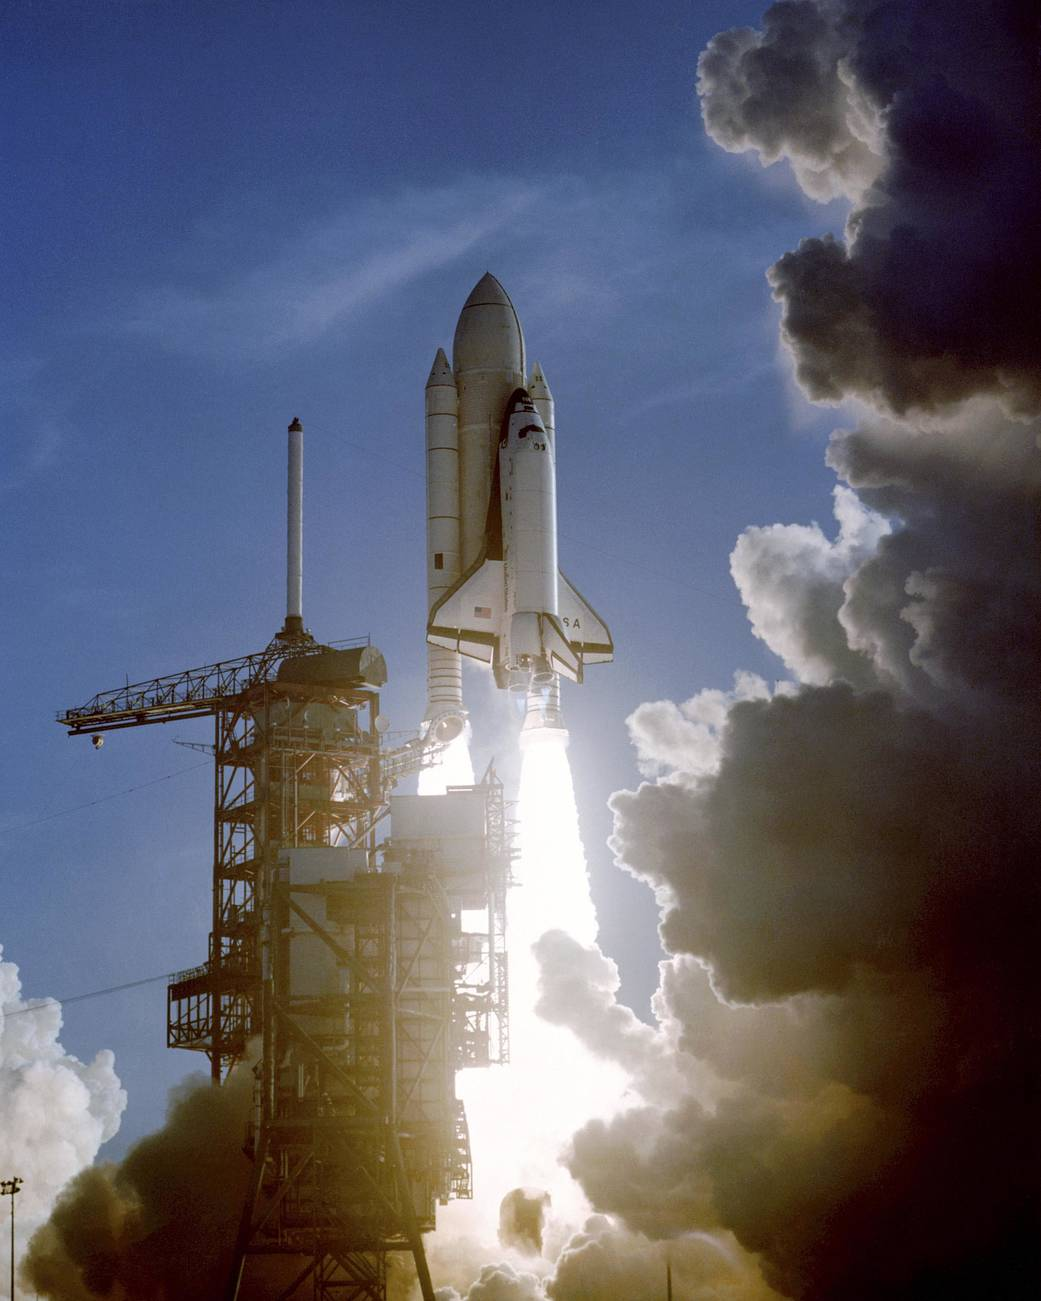
\includegraphics[height=\paperheight]{cover-nasa.jpg}};
\fill[white,opacity=.91] (0,0) rectangle (595.276,89.5);
\fill[studiumInk,opacity=.96] (0,585.5) rectangle (595.276,841.89);
\node[anchor=west,text=studiumInk,font=\sffamily\bfseries\fontsize{18}{20}\selectfont,inner sep=0pt] at (51.223,38.5){STUDIUM};
\fill[studiumCyan] (51.223,61.5) rectangle (80.8,63.7);
\node[anchor=west,text=studiumInk,font=\sffamily\fontsize{9}{11}\selectfont,inner sep=0pt] at (89.49,65.5){BIBLIOTECA DE INGENIERÍA};
\node[anchor=west,text=studiumCyan,font=\sffamily\bfseries\fontsize{10}{12}\selectfont,inner sep=0pt] at (51.223,608){MANUAL UNIVERSITARIO};
\node[anchor=north west,text=white,text width=493pt,font=\rmfamily\bfseries\fontsize{33}{36}\selectfont,inner sep=0pt] at (51.223,636){#1};
\node[anchor=west,text=white!82!studiumInk,font=\sffamily\fontsize{11}{14}\selectfont,inner sep=0pt] at (51.223,732){#2};
\node[anchor=west,text=white,font=\sffamily\bfseries\fontsize{10}{12}\selectfont,inner sep=0pt] at (51.223,758){GRADO EN INGENIERÍA AEROESPACIAL};
\node[anchor=west,text=white!82!studiumInk,font=\sffamily\fontsize{10}{12}\selectfont,inner sep=0pt] at (51.223,773){Universidad de León};
\draw[white!75!studiumInk,line width=.4pt] (51.223,786) -- (544.05,786);
\node[anchor=west,text=white!82!studiumInk,font=\sffamily\fontsize{10}{12}\selectfont,inner sep=0pt] at (51.223,810){2026};
\node[anchor=east,text=white,font=\sffamily\bfseries\fontsize{10}{12}\selectfont,inner sep=0pt] at (544.05,810){I Edición};
\end{scope}\end{tikzpicture}\null\end{titlepage}\hypersetup{pageanchor=true}}

\hypersetup{pdftitle={Tecnología Aeroespacial. Fundamentos, sistemas y principios del vuelo},pdfauthor={Daniel Miguel Tejedor}}
\renewcommand{\studiumvolumetype}{manual}
\begin{document}
\studiumcover{TECNOLOGÍA\\AEROESPACIAL}{Fundamentos, sistemas y principios del vuelo}{MANUAL UNIVERSITARIO}
\frontmatter
\studiumreadingguide
\chapter*{Presentación y alcance}
Este libro desarrolla los fundamentos de Tecnología Aeroespacial para segundo curso del Grado en Ingeniería Aeroespacial de la Universidad de León. Su organización en 25 capítulos es editorial: la guía oficial del curso 2026/2027 contiene 13 temas. Los bloques, resultados de aprendizaje y criterios de evaluación se han contrastado con la guía docente descargada. Esta es una edición de estudio independiente, sin atribuir aprobación institucional. Las comprobaciones realizadas y su alcance se detallan en el expediente.

Conviene leer primero el modelo físico y sus hipótesis, después seguir la derivación y, finalmente, resolver el ejemplo sin mirar el resultado. Los ejercicios propuestos mezclan cálculo, interpretación y diagnóstico de errores. Un número sin unidades o una fórmula aplicada fuera de dominio no constituye una solución. En actuaciones debe indicarse qué se mantiene fijo al variar una magnitud: peso, altitud, velocidad, configuración o empuje.

El manual incluye ejemplos completos y guías breves para que pueda estudiarse de forma autónoma. El cuaderno de problemas añade 30 casos originales con trazabilidad de cálculo. Los simulacros proponen situaciones integradas y separan enunciados y soluciones. Son materiales editoriales de preparación; no son predicciones del examen ni reproducciones de convocatorias anteriores.

La evaluación oficial asigna 85\,\% a pruebas escritas y 15\,\% a prácticas. El trabajo práctico es imprescindible para optar al proceso de evaluación. La guía admite establecer mínimos por fases, sin fijar aquí una nota que no conste. Las prácticas originales del apéndice entrenan elaboración de informes, comparación de modelos y tratamiento de incertidumbre, y complementan el guion que entregue el profesorado.

\caja{Principio de Studium}{The model is not a source of truth. Las fuentes, las comprobaciones matemáticas y la revisión científica son capas diferentes. Compilar un PDF o reproducir una cuenta no demuestra que todas sus afirmaciones físicas sean correctas.}



\tableofcontents
\listoffigures
\mainmatter
\part{Introducción a la tecnología aeroespacial}
\chapter{Introducción a la ingeniería aeroespacial}\label{ch:01}
\objetivos{Identificar los subsistemas de un vehículo aeroespacial y sus acoplamientos; distinguir masa, fuerza, energía y potencia; construir un modelo elemental de misión y valorar su dominio de aplicación.}

Una aeronave no vuela porque una sola de sus piezas funcione bien. Vuela cuando las fuerzas aerodinámicas, la estructura, la propulsión, el control y los sistemas de a bordo satisfacen simultáneamente las exigencias de una misión. Esta idea organiza la asignatura: aprenderemos el vocabulario y los modelos que permiten dialogar entre especialidades, antes de estudiar cada una con mayor profundidad. La guía de contenidos aportada sitúa precisamente la atmósfera y la mecánica de fluidos antes de la aerodinámica, las actuaciones y los sistemas \cite{TAE0}.

\section{Del propósito al requisito}
Un propósito, como transportar observaciones de un incendio, no es todavía un requisito técnico. Hay que precisar la zona que se quiere cubrir, el tiempo disponible, la carga instrumental, el viento previsto, la autonomía, las condiciones de lanzamiento y recuperación y las consecuencias de un fallo. Una cámara pesada mejora quizá la resolución, pero exige más sustentación y energía. Una aeronave rápida llega antes, aunque necesita más potencia y puede ofrecer menos tiempo de observación. La ingeniería convierte propósitos en magnitudes medibles y explicita los compromisos.

La misión se divide en segmentos: preparación, despegue o lanzamiento, ascenso, tránsito, operación, retorno y recuperación. Cada segmento puede imponer un requisito distinto. El ascenso suele exigir potencia; el despegue, distancia y control a baja velocidad; el crucero, eficiencia; el aterrizaje, disipación de energía y precisión. Diseñar solo para el segmento más largo deja sin resolver condiciones breves que pueden gobernar el tamaño del vehículo.

Un requisito debe indicar qué se mide y bajo qué condiciones. ``Autonomía suficiente'' es ambiguo; ``permanencia de dos horas con una carga de veinte kilogramos bajo unas condiciones atmosféricas definidas'' permite calcular, ensayar y comprobar. También debe haber coherencia entre requisitos: aumentar carga útil, alcance y velocidad manteniendo masa, tamaño y energía rara vez es posible sin introducir una tecnología distinta.

\section{Vehículos y formas de sostenerse}
Los aerostatos se mantienen gracias al empuje de Arquímedes. Un globo no necesita velocidad horizontal para obtener sustentación estática, pero un globo libre se desplaza con la masa de aire. El dirigible añade propulsión y superficies o dispositivos de control. En ambos casos importa la diferencia entre la masa del aire desalojado y la masa completa del vehículo.

Los aerodinos obtienen la mayor parte de su sustentación mediante el movimiento relativo del aire. El avión utiliza alas; el helicóptero, un rotor accionado; el autogiro mantiene el giro de su rotor principalmente por autorrotación y suele disponer de una hélice separada para avanzar. Un rotor puede producir sustentación con el vehículo casi inmóvil respecto al suelo, porque sus palas se mueven respecto al aire. Confundir velocidad del centro de masas con velocidad de las superficies sustentadoras conduce a interpretaciones erróneas.

Los vehículos espaciales añaden otro régimen. En órbita, la sustentación aerodinámica no es el mecanismo de soporte principal: el vehículo está en caída libre y su velocidad tangencial impide que alcance la superficie. Un cohete tampoco se impulsa apoyándose en el aire exterior; expulsa masa y recibe una fuerza de reacción. Durante lanzamiento y reentrada, sin embargo, la atmósfera vuelve a imponer cargas, calentamiento y restricciones de control. La frontera entre ingeniería aeronáutica y astronáutica es una zona de interacción, además de una división administrativa.

\section{Subsistemas y caminos de carga}
El ala transmite las fuerzas del aire a largueros y costillas; estas las llevan al fuselaje, que también aloja carga, personas y equipos. La estructura debe resistir sin deformarse excesivamente y con una masa compatible con la misión. Reducir material puede mejorar prestaciones y, a la vez, aumentar deformaciones que alteran la aerodinámica. El acoplamiento entre ambas disciplinas recibe el nombre de aeroelasticidad.

La planta propulsiva transforma energía almacenada en una acción sobre el flujo. Una hélice acelera una masa de aire relativamente grande con un incremento moderado de velocidad; un reactor utiliza otro reparto entre caudal e incremento de velocidad. La instalación altera resistencias, temperaturas, ruido y distribución de masas. El combustible modifica el peso y el centro de gravedad a medida que se consume.

Los mandos de vuelo producen momentos para orientar el vehículo. Estabilidad significa cómo responde a una perturbación; controlabilidad, si los actuadores y superficies disponibles permiten imponer la evolución deseada. Son propiedades distintas. Los sistemas eléctricos, hidráulicos, neumáticos, de combustible e instrumentación suministran energía e información para que la estructura y la propulsión puedan cumplir su función. Un sensor es parte del sistema físico: tiene errores, retardos y condiciones de funcionamiento.

\figura{aircraft}{Esquema original de una aeronave y sus subsistemas principales. Las llamadas identifican los componentes para interpretar el vehículo como un sistema integrado.}

\section{Magnitudes, unidades y órdenes de magnitud}
La masa $m$ mide inercia y se expresa en kilogramos. El peso $W=mg$ es una fuerza, en newtons. Decir que un aparato ``pesa 920 kg'' es una abreviatura coloquial que debe traducirse a una masa de $920\,\mathrm{kg}$ antes de plantear balances. Cerca de la superficie puede emplearse $g=\gzero\,\mathrm{m\,s^{-2}}$ como referencia, indicando que se desprecia su variación.

La presión es fuerza normal por unidad de área: $1\,\mathrm{Pa}=1\,\mathrm{N\,m^{-2}}$. El trabajo mide transferencia de energía mediante fuerzas a lo largo de un desplazamiento; la potencia mide su rapidez de transferencia. Un motor de mucha potencia no almacena necesariamente mucha energía. La autonomía de una batería requiere conocer su energía utilizable y la potencia demandada durante la misión.

Una comprobación dimensional evita errores graves, pero no demuestra que un modelo sea correcto. Dos expresiones diferentes pueden tener las mismas dimensiones. También hay que comprobar signos, límites y órdenes de magnitud. Una fuerza de sustentación muy inferior al peso no es compatible con un vuelo horizontal estacionario, aunque ambas cantidades estén correctamente expresadas en newtons.

\section{Un primer modelo del vuelo}
En vuelo rectilíneo horizontal estacionario, con empuje aproximadamente paralelo a la trayectoria y sin aceleración, se obtiene
\begin{equation}
 L=W,\qquad T=D.
\end{equation}
Las cuatro fuerzas no son iguales entre sí: la igualdad relaciona cada pareja según su dirección. La sustentación $L$ es perpendicular a la velocidad relativa y la resistencia $D$ es paralela y opuesta a ella. El peso es vertical; el empuje sigue el eje de instalación y puede tener componente vertical.

Definimos la presión dinámica $q=\rho V^2/2$, donde $\rho$ es densidad y $V$ velocidad respecto al aire. Las fuerzas se escriben
\begin{equation}
 L=qSC_L,\qquad D=qSC_D,
\end{equation}
con superficie de referencia $S$ y coeficientes adimensionales. Los coeficientes condensan efectos de forma, orientación y régimen; no son constantes universales. En particular, $C_L$ cambia con el ángulo de ataque hasta que la separación del flujo altera de forma importante su evolución.

La potencia útil para vencer resistencia es $P_u=DV$. Para una hélice de rendimiento $\eta_p$, la potencia al eje resulta $P_e=DV/\eta_p$. Esta relación corresponde a un balance estacionario: durante el ascenso también aumenta la energía potencial y durante una aceleración aumenta la energía cinética. Tampoco sustituye un mapa real de motor o hélice.

\refstepcounter{section}\addcontentsline{toc}{section}{\protect\numberline{\thesection}Problema resuelto: una primera estimación de crucero}
\begin{studiumworked}{Problema resuelto: una primera estimación de crucero}

\begin{enumerate}
\item \textbf{Enunciado.} Un avión de observación debe mantener un tramo horizontal a $55\,\mathrm{m\,s^{-1}}$. Estimar el coeficiente de sustentación, el empuje y la potencia al eje necesarios.
\item \textbf{Datos.} $m=920\,\mathrm{kg}$, $S=16\,\mathrm{m^2}$, $\rho=1.06\,\mathrm{kg\,m^{-3}}$, $C_D=0.038$ y $\eta_p=0.78$.
\item \textbf{Incógnitas.} $C_L$, $T$ y $P_e$ en esa condición de vuelo.
\item \textbf{Esquema verbal.} Sobre el centro de masas actúan peso hacia abajo, sustentación hacia arriba, empuje hacia delante y resistencia hacia atrás.
\item \textbf{Hipótesis.} Movimiento estacionario, ausencia de viento vertical, empuje horizontal, densidad uniforme y coeficiente de resistencia válido en la condición calculada.
\item \textbf{Modelo.} Equilibrio de fuerzas y definición de coeficientes aerodinámicos.
\item \textbf{Ecuaciones.} $q=\rho V^2/2$, $qSC_L=mg$, $T=qSC_D$, $P_e=TV/\eta_p$.
\item \textbf{Despeje.} $C_L=2mg/(\rho V^2S)$ y $P_e=\rho V^3SC_D/(2\eta_p)$.
\item \textbf{Sustitución.} $q=1603.25\,\mathrm{Pa}$, $W=9022.12\,\mathrm{N}$ y $qS=25652\,\mathrm{N}$.
\item \textbf{Resultado.} $C_L=0.352$, $T=974.8\,\mathrm{N}$ y $P_e=68.7\,\mathrm{kW}$, con redondeo coherente con los datos.
\item \textbf{Interpretación.} La potencia útil es $53.6\,\mathrm{kW}$; el resto de la potencia al eje se pierde respecto a la producción de trabajo propulsivo útil según el rendimiento adoptado.
\item \textbf{Comprobación independiente.} La eficiencia aerodinámica es $L/D=9.26$; entonces $W/(L/D)=974.8\,\mathrm{N}$, igual al empuje calculado.
\item \textbf{Limitaciones.} No se han comprobado pérdida, estabilidad, capacidad del motor a esa altitud ni cambios de $C_D$ con $C_L$. El resultado dimensiona una condición, no certifica una aeronave.
\end{enumerate}

\end{studiumworked}

\section{Cómo se construye una justificación técnica}
La verificación pregunta si un cálculo o sistema satisface las especificaciones elegidas; la validación pregunta si esas especificaciones y modelos representan adecuadamente el propósito real. Un programa puede resolver con precisión una ecuación inapropiada. Por eso se documentan fuentes, unidades, hipótesis, incertidumbres y comprobaciones independientes. Cuando una medición contradice el cálculo, se revisan ambos; no se ajustan datos sin justificarlo.

La incertidumbre puede proceder de la medición, de parámetros variables o de simplificaciones del modelo. Si se estima potencia con un $C_D$ poco conocido, obtener seis cifras decimales no añade información. Una sensibilidad elemental muestra que, manteniendo los demás parámetros, $P_e$ varía con $V^3$: un pequeño cambio de velocidad puede afectar mucho a la demanda. Esta observación orienta qué dato conviene medir mejor.

\section{Ejercicios propuestos}
\begin{enumerate}
\item \textbf{Básico.} Convertir una masa de $1250\,\mathrm{kg}$ en peso con gravedad estándar y distinguir sus unidades.
\item \textbf{Intermedio.} Si en el problema anterior la velocidad aumenta un $10\%$ y se mantienen $C_D$, densidad y rendimiento, calcular el factor de aumento de potencia.
\item \textbf{Examen.} Una misión exige $40\,\mathrm{kW}$ útiles durante $90$ minutos. Con rendimiento global del $80\%$, estimar energía mínima de entrada en kilovatios hora y megajulios. Explicar por qué no incluye reserva.
\item \textbf{Conceptual.} Proponer dos motivos por los que una mejora aislada de motor no garantiza una mejora de autonomía.
\end{enumerate}
\section{Respuestas y orientación}
1. $12258.3\,\mathrm{N}$; kilogramo y newton no son intercambiables. 2. $1.1^3=1.331$, un $33.1\%$. 3. $75\,\mathrm{kWh}=270\,\mathrm{MJ}$; faltan reservas y segmentos adicionales. 4. Por ejemplo, aumento de masa o funcionamiento fuera del punto eficiente; se debe explicar el acoplamiento.

\resumen{La misión genera requisitos y cada subsistema condiciona a los demás. Los balances elementales de fuerzas y energía permiten estimaciones útiles si se explicitan sus hipótesis. Masa y peso, potencia y energía, velocidad aérea y velocidad respecto al suelo son magnitudes diferentes. Un resultado técnico debe conservar unidades, mostrar sus límites y admitir una comprobación independiente.}
\section{Autoevaluación}
\begin{enumerate}
\item ¿Qué requisito podría dimensionar el motor aunque el crucero dure más tiempo?
\item ¿Por qué un coeficiente adimensional puede variar entre dos ensayos?
\item ¿Qué diferencia hay entre comprobar una ecuación y comprobar su aplicabilidad?
\end{enumerate}


\studiumchaptercheck
\chapter{Historia de la aviación y de la carrera espacial}\label{ch:02}
\objetivos{Relacionar los hitos históricos con los problemas técnicos que resolvieron; distinguir demostración, capacidad operativa y explotación sostenida; analizar fuentes sin convertir una cronología en una explicación causal.}

La historia aeroespacial permite reconocer un patrón: una idea físicamente posible puede tardar décadas en convertirse en un sistema práctico. Para volar se necesitaban conocimientos de fuerzas y materiales, pero también motores suficientemente ligeros, mecanismos de control y una forma organizada de ensayar. Para alcanzar la órbita hicieron falta propulsión, guiado, estructuras y una infraestructura capaz de integrarlos. Este capítulo desarrolla la secuencia presentada en los materiales de la asignatura y la interpreta como historia de problemas de ingeniería \cite{TAE1}.

\section{Antes del vuelo: imaginar, medir y separar funciones}
Los relatos de vuelo expresan un deseo humano; no constituyen evidencia de que sus protagonistas dispusieran de máquinas capaces de cumplirlo. Algo parecido ocurre con los dibujos de Leonardo da Vinci: son relevantes para estudiar imaginación mecánica y observación de las aves, pero un dibujo no equivale a una demostración experimental. La distinción entre propuesta y realización seguirá siendo necesaria al evaluar vehículos contemporáneos.

La imitación directa de un pájaro plantea dificultades de escala, potencia muscular y complejidad mecánica. El paso decisivo hacia el avión consistió en separar funciones. Un elemento produce sustentación, otro proporciona propulsión y otros permiten estabilizar y orientar. En los trabajos de George Cayley aparece esa lectura funcional del vehículo. No hacía falta reproducir todos los movimientos de un ave para satisfacer las mismas leyes físicas.

Los planeadores permitieron estudiar el vuelo sin añadir inmediatamente el problema del motor. Las experiencias de Otto Lilienthal mostraron el valor de repetir ensayos y relacionar forma, incidencia y fuerza aerodinámica, aunque también pusieron de manifiesto los riesgos de un control limitado. Un planeador es un laboratorio en movimiento: su fuente de energía es la disminución de energía potencial, y su duración depende tanto de la resistencia como del entorno atmosférico.

\section{Aerostación y vuelo dirigido}
Los globos de aire caliente de finales del siglo XVIII demostraron que sostener una carga en el aire no exigía necesariamente alas. Su principio era conocido en hidrostática, pero hacerlo operativo requería fabricar una envolvente ligera, producir calentamiento y controlar fugas y cargas. El logro técnico fue una integración de materiales y procedimientos, además de una aplicación de Arquímedes.

El globo libre no podía imponer una trayectoria horizontal respecto al aire. Incorporar una hélice dio lugar a un problema nuevo: conseguir que el empuje superase una resistencia considerable sin añadir demasiada masa. Los dirigibles combinaron gradualmente envolventes, estructuras, motores y superficies de control. Una gran estructura rígida puede conservar la forma y distribuir cargas, pero aumenta complejidad y masa; una envolvente flexible es más sencilla y necesita mantener condiciones internas compatibles con su forma.

Comparar globos, dirigibles y aviones como si pertenecieran a una única competición de velocidad oculta sus propósitos distintos. La permanencia, la carga y la necesidad de infraestructura pueden favorecer soluciones diferentes. La historia no es una escalera en la que toda tecnología nueva elimina a la anterior: cambian los compromisos y los espacios de aplicación.

\section{Los Wright: el vuelo como problema de integración}
La NASA sitúa el vuelo pilotado, controlado y autopropulsado de los hermanos Wright el 17 de diciembre de 1903. Su explicación destaca una secuencia de investigación: revisión de antecedentes, planeadores, ensayos en túnel, mejora del control y desarrollo de la propulsión. El planeador de 1902 incorporó control de los tres ejes; el aparato de 1903 añadió motor y hélices \cite{NASA-BGA}. La formulación completa del hito importa: decir únicamente ``primer objeto que voló'' excluiría sin motivo los aerostatos y los planeadores anteriores.

La enseñanza de ingeniería que extraemos es que la capacidad de sostenerse no basta para realizar una misión. Un aparato que produce más sustentación que su peso, pero no permite controlar la orientación, puede abandonar el suelo y seguir siendo impracticable. La realimentación experimental también es esencial: si una tabla de datos no predice los resultados del prototipo, hay que revisar el ensayo, su escala y la interpretación del coeficiente.

La hélice puede entenderse como un conjunto de alas rotatorias. Ese vínculo explica que mejorar conocimientos aerodinámicos de perfiles beneficie también a la propulsión. Es un ejemplo temprano de transferencia entre subsistemas. El éxito de la integración no elimina la contribución de precursores; muestra que los conocimientos parciales adquieren otro valor al combinarse en un vehículo controlable.

\section{Del prototipo al transporte y al rotor}
Durante las primeras décadas del siglo XX evolucionaron mandos, alas, estructuras y motores. Las estructuras arriostradas ofrecían ligereza con materiales disponibles, a costa de resistencia adicional de montantes y cables. El progreso hacia revestimientos resistentes permitió distribuir cargas de otra forma. Esta evolución no se explica solo por una mejor forma exterior: dependió de materiales, fabricación, cálculo y experiencia de servicio.

Las guerras aceleraron inversión y producción, pero imponer un requisito militar de velocidad o maniobra no equivalía a optimizar transporte civil. Un servicio comercial necesita regularidad, mantenimiento, economía e infraestructura. El desarrollo de la aviación comercial de hélice, cuyo panorama docente ilustra el DC-3, exige por ello estudiar el sistema de explotación además del avión \cite{TAE1}.

El autogiro desarrollado por Juan de la Cierva introdujo soluciones decisivas para un rotor cuyas palas avanzan y retroceden respecto a la corriente. La articulación permite acomodar diferencias de carga. En autorrotación la energía que mantiene el giro procede del flujo a través del rotor; en un helicóptero durante vuelo estacionario ordinario procede del motor. Atribuir la invención de todo el helicóptero a una única persona simplifica un proceso con numerosos desarrollos; Sikorsky fue una figura destacada en la consolidación de una configuración práctica, no el origen de toda idea de ala rotatoria.

\section{Reacción y vuelo rápido}
La propulsión a reacción hizo posible otra combinación de velocidad y altitud. Los desarrollos de Whittle y von Ohain ilustran que un mismo principio físico puede madurar en trabajos independientes. Una turbina de gas integra compresor, combustión y turbina: el reto no es simplemente encender combustible, sino mantener un balance de potencia y un funcionamiento estable con materiales sometidos a temperaturas altas.

Al acercarse a Mach uno aparecen regiones supersónicas y ondas de choque, aunque la velocidad de la aeronave sea todavía subsónica. La llamada barrera del sonido reunió problemas distintos: aumento de resistencia, cambios de momentos, control y cargas. No era una pared material. Comprender la compresibilidad permitió formular soluciones de ala, entrada y propulsión que no se obtenían extrapolando directamente ensayos lentos.

El transporte supersónico mostró que demostrar velocidad no equivale a alcanzar cualquier objetivo económico. Consumo, ruido, mantenimiento y restricciones operativas afectan a la viabilidad. Esta observación es histórica y metodológica: no se deduce que una capacidad carezca de valor porque no se extienda a todos los mercados.

\section{De la astronomía a la órbita}
La observación astronómica produjo modelos cada vez más precisos del movimiento celeste. El heliocentrismo, las leyes de Kepler y la gravitación permitieron describir órbitas con una base matemática. Sin embargo, calcular una trayectoria no proporciona automáticamente un vehículo para recorrerla. La astronáutica necesitó, además, tecnologías de propulsión y control capaces de impartir gran velocidad y resistir el lanzamiento.

La ecuación del cohete vincula incremento de velocidad ideal, velocidad efectiva de escape y razón de masas. Explica por qué expulsar masa funciona en el vacío y por qué la masa estructural es crítica. El empleo de etapas permite abandonar estructuras ya innecesarias. La dificultad de alcanzar órbita no consiste principalmente en subir unos cientos de kilómetros, sino en adquirir una velocidad horizontal elevada sin agotar el vehículo en el proceso.

El contexto de Guerra Fría conectó lanzadores, misiles, prestigio y ciencia. Sputnik 1 fue puesto en órbita el 4 de octubre de 1957; Explorer 1 siguió en 1958 y aportó observaciones asociadas a los cinturones de radiación. NASA comenzó su actividad en octubre de 1958 \cite{NASA-HISTORY}. Estos datos no significan que toda investigación espacial fuese únicamente una aplicación militar: describen un contexto de financiación y competencia con objetivos simultáneos.

\section{Vuelo humano, exploración y continuidad}
El vuelo de Yuri Gagarin en 1961 estableció el primer vuelo espacial humano orbital. Una trayectoria suborbital, como la inicial de Alan Shepard, demuestra capacidades diferentes: supera grandes altitudes sin completar una órbita. Comparar ambos hitos exige definir el criterio, no únicamente contar días entre lanzamientos \cite{TAE1}.

Apollo 11 llevó a Armstrong, Aldrin y Collins a la Luna en julio de 1969; Armstrong y Aldrin descendieron a la superficie y Collins permaneció en órbita lunar \cite{NASA-HISTORY}. El regreso era parte central del objetivo. La misión integró navegación, encuentros orbitales, comunicaciones, soporte vital y protección térmica; un lanzador potente era necesario, pero insuficiente.

Las estaciones orbitales y las sondas ampliaron la permanencia y la investigación. Los satélites de observación, comunicaciones y navegación muestran que la utilidad de una misión no se mide solo por su distancia. También cuentan cobertura, precisión, duración y disponibilidad de los datos. La historia permite reconocer distintas nociones de éxito sin reducirlas a una sola lista de primeros puestos.

\refstepcounter{section}\addcontentsline{toc}{section}{\protect\numberline{\thesection}Caso resuelto: valorar una propuesta histórica}
\begin{studiumworked}{Caso resuelto: valorar una propuesta histórica}

\begin{enumerate}
\item \textbf{Enunciado.} Un estudio ficticio compara dos prototipos de comienzos de la aviación. ¿Basta su potencia específica para decidir cuál puede realizar vuelo controlado?
\item \textbf{Datos.} A dispone de $10\,\mathrm{kW}$ y masa total $260\,\mathrm{kg}$; B de $18\,\mathrm{kW}$ y $310\,\mathrm{kg}$. Solo A tiene ensayos documentados de mandos en tres ejes.
\item \textbf{Incógnitas.} Potencia por masa y conclusión técnica justificable.
\item \textbf{Esquema verbal.} Se comparan capacidad energética e información de control, manteniendo separadas las dos preguntas.
\item \textbf{Hipótesis.} Masas completas comparables y potencias al eje medidas del mismo modo; el ejemplo no representa un aparato histórico concreto.
\item \textbf{Modelo.} Indicador $P/m$ complementado con una evaluación cualitativa de evidencia.
\item \textbf{Ecuación.} $\pi_P=P/m$, cuya unidad es $\mathrm{W\,kg^{-1}}$; no es un coeficiente adimensional.
\item \textbf{Despeje.} Se divide la potencia de cada prototipo por su propia masa completa.
\item \textbf{Sustitución.} $\pi_{P,A}=10000/260$ y $\pi_{P,B}=18000/310$.
\item \textbf{Resultado.} A ofrece $38.5\,\mathrm{W\,kg^{-1}}$ y B $58.1\,\mathrm{W\,kg^{-1}}$; B supera a A en este indicador.
\item \textbf{Interpretación.} No se puede concluir que B realice vuelo controlado. Falta evidencia de sustentación, resistencia, transmisión, estabilidad y autoridad de los mandos.
\item \textbf{Comprobación independiente.} La razón $(18/10)(260/310)=1.51$ coincide con $\pi_{P,B}/\pi_{P,A}$. La comparación cualitativa se verifica preguntando qué afirmación permite realmente cada documento.
\item \textbf{Limitaciones.} Sin mapas de hélice ni datos aerodinámicos, tampoco se puede afirmar que A vuele. Haber ensayado los mandos reduce una incertidumbre y no resuelve todas las demás.
\end{enumerate}

\end{studiumworked}

\section{Ejercicios propuestos}
\begin{enumerate}
\item \textbf{Básico.} Ordenar planeador, vuelo propulsado controlado y transporte regular por la capacidad adicional que requiere cada transición.
\item \textbf{Intermedio.} Explicar qué información faltaría para comparar dos motores históricos a partir de su masa en seco.
\item \textbf{Examen.} Construir un argumento de ocho líneas sobre por qué llegar al espacio y permanecer en órbita son objetivos diferentes. Incluir una condición física y una consecuencia de diseño.
\item \textbf{Conceptual.} Una fuente atribuye un ``primer vuelo'' sin explicar si estaba tripulado ni si era controlado. ¿Qué comprobaciones documentales haría?
\end{enumerate}
\section{Respuestas y orientación}
1. El motor añade energía sostenida; el servicio regular añade fiabilidad, mantenimiento y operación. 2. Potencia útil, combustible, instalación y duración de funcionamiento, entre otros. 3. La órbita requiere velocidad tangencial compatible con caída libre; la trayectoria suborbital intersecta de nuevo regiones bajas. 4. Precisar definición del hito, fecha, testigos, registros y contexto, y contrastar fuentes.

\resumen{La evolución aeroespacial combina ideas físicas, mediciones, materiales, control e infraestructura. Las fechas ubican hitos; la explicación técnica identifica qué problema se resolvió y qué seguía pendiente. Una demostración no garantiza capacidad operativa, y un indicador favorable no sustituye la integración del vehículo.}
\section{Autoevaluación}
\begin{enumerate}
\item ¿Por qué separar sustentación y propulsión fue una idea fértil?
\item ¿Qué enseñan los Wright sobre el valor de revisar datos experimentales?
\item ¿Cómo cambia una comparación histórica al definir exactamente el éxito?
\end{enumerate}


\studiumchaptercheck

\part{Atmósfera y meteorología}
\chapter{Estructura de la atmósfera}\label{ch:03}
\objetivos{Interpretar las propiedades atmosféricas como campos variables; distinguir referencias de altura; relacionar estructura térmica, equilibrio hidrostático y densidad; aplicar el empuje de Arquímedes con un balance correcto de masas.}

La atmósfera es simultáneamente medio sustentador, fuente de oxígeno para muchos motores, entorno térmico y origen de perturbaciones. Su densidad influye en la sustentación; su temperatura modifica la velocidad del sonido; su presión afecta a instrumentos y cabinas. Para estudiar estas relaciones necesitamos distinguir la atmósfera real, variable en espacio y tiempo, de un modelo estándar usado para comparar resultados. El material docente introduce ambas y organiza las capas por su comportamiento térmico \cite{TAE2}.

\section{Composición y descripción macroscópica}
El aire seco próximo a la superficie contiene aproximadamente un $78\%$ de nitrógeno y un $21\%$ de oxígeno en fracción molar, además de argón y otros constituyentes minoritarios. Es una mezcla, no una sustancia química única. El vapor de agua varía mucho y no debe incluirse como una fracción fija del aire seco. Los aerosoles, las gotas y los cristales de hielo tienen importancia óptica, meteorológica y operativa aunque representen una fracción pequeña de masa.

Una composición aproximada sirve para deducir propiedades de mezcla en ingeniería básica; no constituye una tabla de concentraciones actuales. En particular, no se debe trasladar sin fecha la fracción de dióxido de carbono de una diapositiva a una afirmación sobre el presente. Para este manual, la constante del aire seco $\Raire\,\mathrm{J\,kg^{-1}\,K^{-1}}$ se utiliza como parámetro convencional de cálculo.

La descripción de medio continuo asigna presión $p$, temperatura $T$ y densidad $\rho$ a pequeños volúmenes que contienen muchas moléculas. El volumen debe ser pequeño respecto a las variaciones del fenómeno y grande respecto a la escala molecular. En regiones suficientemente enrarecidas esa separación de escalas falla y se requiere un tratamiento cinético. No existe una altitud única que determine la validez del continuo para cualquier vehículo, porque también interviene su tamaño característico.

Para aire ideal de composición fija,
\begin{equation}\label{eq:03-ideal}
 p=\rho RT.
\end{equation}
La temperatura es absoluta, en kelvin, y la presión es absoluta, medida desde el vacío. La ecuación de estado conecta propiedades de equilibrio, pero no dice cómo varían con la altitud: hacen falta un balance mecánico y una descripción térmica.

\section{Referencias verticales y qué mide una altitud}
La superficie terrestre no es una esfera lisa. Un elipsoide de referencia es una superficie matemática útil para geodesia; el geoide es una superficie equipotencial del campo de gravedad que aproxima un nivel medio global del mar. La altura elipsoidal no coincide en general con la elevación referida al geoide. Para una convención compatible puede escribirse $h_{\mathrm{elip}}=H_{\mathrm{ort}}+N$, donde $N$ es la ondulación del geoide. Las letras de geodesia no deben confundirse con las usadas después para altitud geopotencial.

La altitud verdadera se refiere a la posición respecto al nivel medio del mar; la altura sobre el terreno depende además de la elevación local. Un instrumento barométrico no mide ninguna de ellas directamente: mide presión y la convierte mediante una calibración. La altitud de presión es la altitud que asigna a esa presión la atmósfera estándar; la altitud de densidad hace lo mismo con la densidad. Ambas son propiedades equivalentes de un modelo y no necesariamente la posición geométrica del avión.

La altitud indicada depende de la referencia de presión ajustada en el instrumento. Por tanto, conviene evitar definiciones de ``altitud absoluta'' sin expresar el origen elegido: en distintos contextos ese término se emplea de formas incompatibles. En un problema se escribirá explícitamente ``sobre el terreno'', ``sobre el nivel medio del mar'' o ``geopotencial''.

La variación de gravedad puede incorporarse en una coordenada energética. Si $z$ es altitud geométrica y $r_e$ un radio terrestre de referencia, con $g(z)=g_0[r_e/(r_e+z)]^2$, definimos
\begin{equation}
 g_0H=\int_0^z g(\zeta)\,d\zeta,\qquad H=\frac{r_ez}{r_e+z}.
\end{equation}
Así, $H$ es altitud geopotencial y es ligeramente menor que $z>0$. La utilidad no es cambiar la física, sino escribir el potencial gravitatorio como $g_0H$. Para unos pocos kilómetros la diferencia es pequeña; en cálculos exigentes debe indicarse la coordenada.

\section{Equilibrio hidrostático y masa de una columna}
Consideremos una lámina de aire de área $A$ y espesor $dz$, con $z$ positivo hacia arriba. La presión inferior ejerce $pA$ hacia arriba; la superior, $(p+dp)A$ hacia abajo; el peso es $\rho gA\,dz$. Si la aceleración vertical media es despreciable,
\begin{equation}\label{eq:03-hidro}
 pA-(p+dp)A-\rho gA\,dz=0,
 \qquad \frac{dp}{dz}=-\rho g.
\end{equation}
El signo negativo expresa que hay menos aire por encima cuando ascendemos. La aproximación hidrostática es adecuada para el perfil medio a gran escala; no describe por sí sola una corriente ascendente intensa ni las fluctuaciones de presión alrededor de un ala.

Integrando entre la superficie y un nivel alto cuya presión sea despreciable y tomando $g$ aproximadamente constante,
\begin{equation}
 p_s\simeq g\int_0^\infty\rho\,dz,\qquad \frac{m_{\mathrm{col}}}{A}\simeq\frac{p_s}{g}.
\end{equation}
A $101325\,\mathrm{Pa}$, la masa de la columna es aproximadamente $10332\,\mathrm{kg\,m^{-2}}$. No significa que toda esa masa esté concentrada en un punto; es la integral de una distribución de densidad decreciente.

Combinando hidrostática y gas ideal obtenemos $d\ln p/dz=-g/(RT)$. La escala de altura local $H_s=RT/g$ indica la distancia característica de variación de presión si la temperatura y la gravedad se mantienen constantes. A $288\,\mathrm{K}$ resulta unos $8.4\,\mathrm{km}$. El símbolo $H_s$ no representa la altura total de la atmósfera: una exponencial no se anula a una altura finita.

\section{Capas térmicas y límites variables}
La troposfera es la capa baja en la que, en promedio, la temperatura disminuye con la altura. El calentamiento de la superficie y las transferencias de calor participan en su organización; contiene la mayor parte del vapor de agua y buena parte de la meteorología que afecta al vuelo. Su límite superior, la tropopausa, cambia con latitud, estación y situación meteorológica. Los $11\,\mathrm{km}$ de la atmósfera estándar no deben convertirse en una frontera física universal.

En la estratosfera aparece una región donde la temperatura aumenta con altura, ligada a la absorción de radiación por el ozono. Ese gradiente favorece la estabilidad de movimientos verticales pequeños. Decir que no hay meteorología en ella sería demasiado absoluto: existen ondas, transportes y nubes particulares. Para la comparación introductoria basta señalar que la convección húmeda profunda es característica de la troposfera.

La mesosfera vuelve a presentar una disminución de temperatura. En la termosfera, la absorción de radiación energética aumenta la energía cinética media de partículas muy separadas. Una temperatura cinética alta no equivale a una gran capacidad de calentar un objeto por contacto: el flujo de energía depende también del número de partículas y de su interacción con la superficie. Por eso no se puede estimar el calentamiento de un satélite leyendo solo la temperatura del gas.

La exosfera corresponde a una región tan poco densa que las colisiones dejan de dominar las trayectorias de muchas partículas. Las clasificaciones térmica, composicional y eléctrica se superponen: la ionosfera no es una capa térmica adicional situada simplemente encima de todas las demás. Esta distinción importa para comunicaciones y para estudiar el entorno espacial.

\section{Transferencia de calor y balance radiativo}
La conducción transfiere energía por interacciones microscópicas y puede modelarse mediante $\boldsymbol{q}=-k\nabla T$. La convección combina transporte de masa y energía interna; la radiación transporta energía electromagnética y no necesita un medio material. En una pared de aeronave pueden actuar las tres simultáneamente. Identificar el mecanismo no obliga a suponer que los demás sean nulos.

Como ejercicio de escala planetaria, la Tierra intercepta radiación sobre un disco de área $\pi r_e^2$, pero reparte emisión sobre un área aproximada $4\pi r_e^2$. Si $S_0$ es irradiancia solar y $\alpha$ albedo, un balance global idealizado da
\begin{equation}
 (1-\alpha)S_0\pi r_e^2=4\pi r_e^2\sigma T_e^4,
 \qquad T_e=\left[\frac{(1-\alpha)S_0}{4\sigma}\right]^{1/4}.
\end{equation}
Con $S_0=1361\,\mathrm{W\,m^{-2}}$ y $\alpha=0.30$ como parámetros ilustrativos, $T_e$ es aproximadamente $255\,\mathrm{K}$. Es una temperatura efectiva de emisión de un modelo agregado, no una predicción directa de la temperatura del suelo. La absorción atmosférica y la distribución vertical requieren un balance más rico \cite{TAE2}.

Las estaciones resultan principalmente de la inclinación del eje terrestre: cambian duración del día y ángulo de incidencia. La variación de distancia al Sol no explica por sí sola que ambos hemisferios tengan estaciones opuestas. Esta geometría condiciona el calentamiento diferencial que, a su vez, impulsa circulaciones atmosféricas.

\section{Densidad del aire húmedo y flotabilidad}
Para una mezcla ideal de aire seco y vapor, $p=p_d+e$ y
\begin{equation}
 \rho=\frac{p-e}{R_dT}+\frac{e}{R_vT}.
\end{equation}
Como $R_v>R_d$, sustituir parte del aire seco por vapor reduce la densidad a iguales presión total y temperatura. La frase ``aire húmedo más pesado'' suele confundir vapor gaseoso con agua líquida suspendida o con cambios simultáneos de temperatura. La fórmula anterior describe vapor sin carga significativa de gotas.

El empuje de Arquímedes sobre un cuerpo de volumen $V$ en una atmósfera aproximadamente uniforme es $B=\rho_a gV$. Para un globo con gas de densidad $\rho_g$ y masa no gaseosa $m_s+m_c$,
\begin{equation}\label{eq:03-globo}
 F_z=(\rho_a-\rho_g)gV-(m_s+m_c)g.
\end{equation}
Esta fuerza neta no es una velocidad de ascenso. Para obtener velocidad harían falta resistencia, masa efectiva y evolución del volumen. En equilibrio estático $F_z=0$ y el gas también tiene masa: omitirla sobreestima la carga disponible.

\refstepcounter{section}\addcontentsline{toc}{section}{\protect\numberline{\thesection}Problema resuelto: margen de sustentación de un globo}
\begin{studiumworked}{Problema resuelto: margen de sustentación de un globo}

\begin{enumerate}
\item \textbf{Enunciado.} Un globo de helio se encuentra en aire con presión y temperatura conocidas. Determinar la fuerza vertical inicial y la carga máxima en equilibrio a ese mismo estado.
\item \textbf{Datos.} $p=85000\,\mathrm{Pa}$, $T=285\,\mathrm{K}$, $V=180\,\mathrm{m^3}$, masa estructural $m_s=90\,\mathrm{kg}$ y carga actual $m_c=60\,\mathrm{kg}$. Para helio, $R_{He}=2077.1\,\mathrm{J\,kg^{-1}\,K^{-1}}$.
\item \textbf{Incógnitas.} $F_z$ y $m_{c,\max}$, sin incluir márgenes operativos.
\item \textbf{Esquema verbal.} Empuje exterior hacia arriba y pesos de helio, estructura y carga hacia abajo.
\item \textbf{Hipótesis.} Aire seco y helio ideales; igual presión y temperatura dentro y fuera; densidades uniformes; envolvente de volumen conocido; ausencia de viento vertical y de fuerzas de amarre.
\item \textbf{Modelo.} Hidrostática para el empuje y gas ideal para ambas densidades.
\item \textbf{Ecuaciones.} $\rho_a=p/(R_dT)$, $\rho_{He}=p/(R_{He}T)$ y ecuación \eqref{eq:03-globo}.
\item \textbf{Despeje.} $m_{c,\max}=(\rho_a-\rho_{He})V-m_s$.
\item \textbf{Sustitución.} $\rho_a=85000/(287.05287\cdot285)=1.0390\,\mathrm{kg\,m^{-3}}$ y $\rho_{He}=0.14359\,\mathrm{kg\,m^{-3}}$.
\item \textbf{Resultado.} $F_z=+109.6\,\mathrm{N}$ y $m_{c,\max}=71.2\,\mathrm{kg}$. El signo positivo se refiere a la vertical ascendente.
\item \textbf{Interpretación.} La carga actual deja un margen estático de masa de $11.2\,\mathrm{kg}$ en el estado especificado. No es una reserva recomendada para operación real.
\item \textbf{Comprobación independiente.} El aire desalojado tiene masa $187.02\,\mathrm{kg}$ y el helio $25.85\,\mathrm{kg}$. La diferencia con $150\,\mathrm{kg}$ de masas no gaseosas es $11.17\,\mathrm{kg}$, cuyo peso coincide con la fuerza neta.
\item \textbf{Limitaciones.} Al ascender variarán presión, volumen y temperatura. No se ha calculado la altitud de equilibrio ni el límite de expansión de la envolvente.
\end{enumerate}

\par\textbf{Procedimiento completo para comparar tu solución.} Obtener densidades con el gas ideal a la misma presión y temperatura. Arquímedes compensa peso del helio, estructura y carga; al dividir por gravedad, la masa adicional es $(\rho_a-\rho_{He})V-m_s-m_c$.

\begin{enumerate}

\item Densidad de aire exterior.

\[\fitmath{\mathrm{rhoa}=\frac{85000}{287.05287\cdot 285}\approx 1.038992\,\mathrm{kg/m^{3}}}\]

\item Densidad de helio.

\[\fitmath{\mathrm{rhoHe}=\frac{85000}{2077.1\cdot 285}\approx 0.1435875\,\mathrm{kg/m^{3}}}\]

\item Restar masa de gas de la masa de aire desplazada.

\[\fitmath{\mathrm{mnet}=\left(\mathrm{rhoa}-\mathrm{rhoHe}\right)\cdot 180}\]

\[\fitmath{\mathrm{mnet}=\left((1.038991925)-(0.1435875086)\right)\cdot 180\approx 161.1728\,\mathrm{kg}}\]

\item Descontar estructura y la carga ya embarcada.

\[\fitmath{\mathrm{mextra}=\mathrm{mnet}-90-60}\]

\[\fitmath{\mathrm{mextra}=(161.172795)-90-60\approx 11.17279\,\mathrm{kg}}\]

\end{enumerate}

\end{studiumworked}

\section{De un perfil medio a una atmósfera real}
Un perfil vertical describe un lugar y un instante, mientras que una estructura media resume muchos estados. Las inversiones térmicas cerca del suelo, las corrientes en chorro y los sistemas frontales pueden producir diferencias importantes entre puntos próximos. Un avión no encuentra únicamente un valor de densidad: atraviesa gradientes y perturbaciones que generan cargas y errores de medida. Por eso los modelos de actuaciones y los modelos de ráfagas responden a preguntas distintas.

También debe distinguirse el aire que rodea al vehículo del que se ha frenado o comprimido en una entrada o sobre un sensor. La temperatura estática ambiental y la temperatura de remanso no coinciden durante movimiento rápido. Utilizar la segunda como si fuera un sondeo atmosférico sobreestima la temperatura de la corriente libre. La instrumentación necesita un modelo del proceso de medida además de un modelo de la atmósfera.

\section{Ejercicios propuestos}
\begin{enumerate}
\item \textbf{Básico.} Hallar densidad de aire seco a $90000\,\mathrm{Pa}$ y $300\,\mathrm{K}$. Compararla con el mismo aire a $280\,\mathrm{K}$ y presión fija.
\item \textbf{Intermedio.} Calcular la masa de una columna por unidad de área a $90000\,\mathrm{Pa}$ con gravedad estándar.
\item \textbf{Examen.} Un globo flexible cerrado mantiene gas ideal a la temperatura exterior y presión exterior durante un ascenso. Mostrar que $\rho_aV=m_gR_g/R_a$ es constante si no varía la composición. Explicar por qué el equilibrio no queda determinado solo por la disminución de densidad del aire.
\item \textbf{Conceptual.} ¿Puede un satélite estar en una región de temperatura cinética muy alta y recibir poco calor por colisiones? Justificar.
\end{enumerate}
\section{Respuestas y orientación}
1. $1.0451$ y $1.1198\,\mathrm{kg\,m^{-3}}$: a presión fija, calentar disminuye densidad. 2. $9177.4\,\mathrm{kg\,m^{-2}}$. 3. Usar $pV=m_gR_gT$ y $\rho_a=p/(R_aT)$; la expansión compensa la disminución de densidad hasta que falla alguna hipótesis. 4. Sí: temperatura y flujo de energía no son la misma magnitud; importa la densidad y la interacción con la superficie.

\resumen{La atmósfera presenta una estructura térmica variable y distintas referencias de altura. Hidrostática, composición y ecuación de estado permiten relacionar presión, temperatura y densidad, pero requieren un cierre térmico. La flotabilidad depende de la masa de aire desalojado menos todas las masas del vehículo, incluido el gas. La temperatura por sí sola no determina una transferencia de calor.}
\section{Autoevaluación}
\begin{enumerate}
\item ¿Qué representa físicamente la presión de una columna atmosférica?
\item ¿Por qué la altitud de densidad no es necesariamente una posición geométrica?
\item ¿Qué hipótesis impide usar directamente este modelo de globo para calcular su velocidad terminal?
\end{enumerate}


\studiumchaptercheck
\chapter{Atmósfera estándar ISA}\label{ch:04}
\objetivos{Derivar los perfiles de presión y densidad en capas de gradiente térmico constante; enlazar capas sin discontinuidades artificiales; calcular velocidades y altitudes equivalentes; distinguir un modelo de referencia de un sondeo meteorológico.}

Un avión ensayado en un día frío y otro cálido no opera en el mismo medio, aunque esté a la misma altitud. Para comparar actuaciones e instrumentos necesitamos una referencia común. La atmósfera estándar prescribe temperatura, presión y densidad en función de una coordenada vertical. No pronostica el tiempo ni supone que el aire real siga siempre sus valores. Los apuntes de la asignatura presentan las tablas ISA; aquí deducimos sus relaciones para poder utilizarlas sin memorizar números aislados \cite{TAE2,ISA1976}.

\section{Hipótesis y condiciones de referencia}
En la región baja modelamos aire seco, ideal, de composición fija y en equilibrio hidrostático. La temperatura se prescribe por tramos lineales de altitud geopotencial $H$; la ecuación de estado y la hidrostática proporcionan el resto. Las condiciones de referencia al nivel cero son
\begin{align}
 T_0&=288.15\,\mathrm{K},& p_0&=101325\,\mathrm{Pa},\\
 R&=\Raire\,\mathrm{J\,kg^{-1}\,K^{-1}},& g_0&=\gzero\,\mathrm{m\,s^{-2}}.
\end{align}
De ellas resulta $\rho_0=p_0/(RT_0)\simeq1.2250\,\mathrm{kg\,m^{-3}}$. El valor de densidad es una consecuencia de los parámetros, no un dato independiente que pueda cambiarse manteniendo los demás.

La atmósfera estándar de 1976 ofrece un desarrollo más extenso; utilizamos aquí las relaciones de la región donde el modelo de gas de composición constante es apropiado. No se deben extrapolar esas hipótesis hasta cualquier altitud. La denominación ISA es habitual en problemas aeronáuticos; para constantes y estructura de capas se indica la referencia estándar utilizada \cite{ISA1976}.

Si se trabaja con altitud geométrica $z$, se convierte primero mediante $H=r_ez/(r_e+z)$. Si el problema declara ``altitud ISA'' sin otra aclaración y pretende un cálculo introductorio, puede adoptarse $H$ como variable, pero se debe escribir. A $11\,\mathrm{km}$ la diferencia con $z$ es pequeña en términos relativos y ya apreciable frente a una precisión de un metro.

\section{Derivación de una capa con gradiente térmico}
Sea $H_b$ la base de una capa y $\beta=dT/dH$ su gradiente, con signo. La temperatura es
\begin{equation}\label{eq:04-T}
 T=T_b+\beta(H-H_b).
\end{equation}
La troposfera estándar tiene $\beta=-0.0065\,\mathrm{K\,m^{-1}}$. Escribir el signo dentro de la definición evita alternar sin aviso entre un gradiente negativo y una tasa de descenso positiva.

Por la definición de altitud geopotencial, la ecuación hidrostática se convierte en $dp/dH=-\rho g_0$. Al sustituir $\rho=p/(RT)$,
\begin{equation}
 \frac{dp}{p}=-\frac{g_0\,dH}{R[T_b+\beta(H-H_b)]}.
\end{equation}
Integrando entre la base y el punto, para $\beta\ne0$,
\begin{equation}\label{eq:04-p}
 \ln\frac{p}{p_b}=-\frac{g_0}{R\beta}\ln\frac{T}{T_b},\qquad
 p=p_b\left(\frac{T}{T_b}\right)^{-g_0/(R\beta)}.
\end{equation}
El exponente es adimensional: $R\beta$ tiene unidades de aceleración. Con $\beta<0$, la temperatura decrece y el exponente es positivo, por lo que también disminuye la presión. La densidad se obtiene sin una nueva integración:
\begin{equation}\label{eq:04-rho}
 \frac{\rho}{\rho_b}=\left(\frac{T}{T_b}\right)^{-g_0/(R\beta)-1}.
\end{equation}
En la primera capa el exponente de presión es aproximadamente $5.2559$ y el de densidad $4.2559$. Estas potencias proceden de un modelo térmico lineal, no de una ley universal para cualquier atmósfera.

\section{Capa isoterma y unión de capas}
Cuando $\beta=0$ no se debe sustituir directamente en una expresión que divide por $\beta$. Se integra de nuevo con $T=T_b$:
\begin{equation}\label{eq:04-iso}
 p=p_b\exp\left[-\frac{g_0(H-H_b)}{RT_b}\right],\qquad
 \rho=\rho_b\exp\left[-\frac{g_0(H-H_b)}{RT_b}\right].
\end{equation}
La presión nunca llega a cero a una distancia finita en esta capa idealizada. Puede comprobarse además que la expresión exponencial es el límite de la capa lineal cuando $\beta\to0$, usando $\ln(1+x)\simeq x$.

En $H=11000\,\mathrm{m}$, la primera capa da $T_b=216.65\,\mathrm{K}$ y $p_b\simeq22632.1\,\mathrm{Pa}$. Esos valores son la base del tramo isotermo de $11$ a $20\,\mathrm{km}$. La base de una capa no se vuelve a inicializar con la presión al nivel del mar. Hacerlo introduciría un salto de presión y violaría el equilibrio del modelo.

Los siguientes gradientes de referencia son $+1.0\,\mathrm{K\,km^{-1}}$ entre $20$ y $32\,\mathrm{km}$, $+2.8$ entre $32$ y $47$, cero entre $47$ y $51$, $-2.8$ entre $51$ y $71$ y $-2.0$ entre $71$ y $84.852\,\mathrm{km}$ geopotenciales. En cada frontera se conserva continuidad de $T$, $p$ y $\rho$. El gradiente sí cambia por la idealización a tramos. Esta lista es un mapa para elegir la ecuación; no se exige reproducir todos sus valores de memoria para comprender el método. En U.S. Standard Atmosphere 1976, el perfil lineal de los últimos tramos se define para temperatura molecular de referencia. Hasta unos $80\,\mathrm{km}$ coincide con la temperatura cinética; entre $80$ y $86\,\mathrm{km}$ geométricos aparece una pequeña corrección de masa molecular. Nuestros cálculos resueltos se mantienen por debajo de $20\,\mathrm{km}$, donde esa distinción no interviene.

\figura{isa}{Perfiles originales de temperatura, presión y densidad de la atmósfera de referencia. Se identifican las bases de capa y se distingue temperatura lineal de presión no lineal.}

\section{Velocidad del sonido y otras propiedades}
Para una perturbación acústica pequeña en aire caloríficamente perfecto,
\begin{equation}
 a=\sqrt{\gamma RT},\qquad \gamma\simeq1.4.
\end{equation}
A nivel del mar estándar $a_0\simeq340.3\,\mathrm{m\,s^{-1}}$. A $11\,\mathrm{km}$ resulta aproximadamente $295.1\,\mathrm{m\,s^{-1}}$. No hay una única velocidad del sonido que sirva para todas las altitudes. El número de Mach $M=V/a$ debe calcularse con la temperatura local y con velocidad relativa al aire.

La viscosidad dinámica depende de temperatura. Una correlación útil en el rango ordinario del aire es la ley de Sutherland,
\begin{equation}
 \mu=\mu_{\mathrm{ref}}\left(\frac{T}{T_{\mathrm{ref}}}\right)^{3/2}
 \frac{T_{\mathrm{ref}}+S_\mu}{T+S_\mu},
\end{equation}
con $T_{\mathrm{ref}}=273.15\,\mathrm{K}$, $\mu_{\mathrm{ref}}=1.716\times10^{-5}\,\mathrm{Pa\,s}$ y $S_\mu=110.4\,\mathrm{K}$ como conjunto convencional de parámetros. Debe utilizarse dentro del rango de validez de la correlación, sin extenderla a gases reaccionantes. La viscosidad cinemática $\nu=\mu/\rho$ puede aumentar con altitud aunque la viscosidad dinámica disminuya en una capa fría, porque la densidad disminuye más.

\section{Problema inverso: qué altitud corresponde a un estado}
La altitud de presión $H_p$ se obtiene invirtiendo el perfil estándar. Si la presión pertenece a la primera capa,
\begin{equation}\label{eq:04-inv}
 H_p=\frac{T_0}{\beta}\left[\left(\frac{p}{p_0}\right)^{-R\beta/g_0}-1\right].
\end{equation}
Para densidad se invierte la ecuación \eqref{eq:04-rho} en la capa adecuada. Elegir capa es parte del cálculo: una expresión correcta utilizada fuera de su intervalo puede producir un número sin sentido físico.

Supongamos ahora que se conoce $p$ pero el aire está más caliente que el valor estándar a esa presión. Como $\rho=p/(RT)$, su densidad será menor y su altitud de densidad, mayor. Esto ayuda a entender la degradación de sustentación y empuje en condiciones cálidas. No significa necesariamente que la aeronave se haya desplazado hacia arriba.

Escribir ``ISA+$15$'' requiere definir qué se mantiene. Habitualmente se refiere a una temperatura $15\,\mathrm{K}$ superior a la estándar a una altitud de presión especificada. Si se prescribe temperatura desviada a altitud geométrica y se desea un perfil completo de presión, hay que reintegrar la hidrostática con condiciones de contorno consistentes. No es correcto modificar a la vez temperatura y densidad de forma arbitraria.

La ecuación hipsométrica ofrece otro modo de leer la columna atmosférica:
\begin{equation}
 z_2-z_1\simeq\frac{R\overline{T}}{g}\ln\frac{p_1}{p_2},
\end{equation}
cuando $\overline{T}$ representa una media apropiada entre superficies de presión y $g$ se aproxima constante. Una columna fría es más delgada entre las mismas presiones. Este resultado explica por qué una calibración estándar puede sobrestimar la altura real en aire frío, manteniendo la referencia de presión adecuada. Para humedad se usa temperatura virtual en el modelo de aire equivalente.

\refstepcounter{section}\addcontentsline{toc}{section}{\protect\numberline{\thesection}Problema resuelto: cálculo de una condición a 4.5 km}
\begin{studiumworked}{Problema resuelto: cálculo de una condición a 4.5 km}

\begin{enumerate}
\item \textbf{Enunciado.} Para interpretar un ensayo de vuelo, determinar temperatura, presión, densidad y velocidad del sonido a $4500\,\mathrm{m}$ de altitud geopotencial estándar. Hallar también el Mach a $140\,\mathrm{m\,s^{-1}}$.
\item \textbf{Datos.} Constantes de referencia de este capítulo, $\beta=-0.0065\,\mathrm{K\,m^{-1}}$ y $\gamma=1.4$.
\item \textbf{Incógnitas.} $T$, $p$, $\rho$, $a$ y $M$.
\item \textbf{Esquema verbal.} Se asciende dentro de una única capa desde la base $H=0$ hasta el nivel de ensayo, sin cruzar la tropopausa estándar.
\item \textbf{Hipótesis.} Aire seco ideal y estándar, equilibrio hidrostático, altitud geopotencial dada y calores específicos constantes para el cálculo acústico.
\item \textbf{Modelo.} Capa lineal ISA y ecuación de estado.
\item \textbf{Ecuaciones.} \eqref{eq:04-T}, \eqref{eq:04-p}, $\rho=p/(RT)$, $a=\sqrt{\gamma RT}$ y $M=V/a$.
\item \textbf{Despeje.} Las variables se calculan en ese orden; no es necesario resolver simultáneamente un sistema no lineal.
\item \textbf{Sustitución.} Las expresiones numéricas son
\[
 T=288.15-0.0065\cdot4500=258.90\,\mathrm{K},
\]
\[
 p=101325(258.90/288.15)^{5.25588}\,\mathrm{Pa}.
\]
\item \textbf{Resultado.} $p=57.728\,\mathrm{kPa}$, $\rho=0.77677\,\mathrm{kg\,m^{-3}}$, $a=322.56\,\mathrm{m\,s^{-1}}$ y $M=0.434$.
\item \textbf{Interpretación.} La densidad es aproximadamente el $63.4\%$ de la estándar al nivel del mar. El ensayo a esta velocidad no debe tratarse automáticamente como incompresible sin valorar la precisión buscada.
\item \textbf{Comprobación independiente.} La ley de densidad proporciona $\rho/\rho_0=(258.90/288.15)^{4.25588}$, igual al resultado de $p/(RT)$. La inversión de \eqref{eq:04-inv} recupera $4500\,\mathrm{m}$.
\item \textbf{Limitaciones.} El cálculo no describe la meteorología real del día y no incluye humedad, perfiles anómalos ni errores instrumentales.
\end{enumerate}

Como ejemplo de unión de capas, a $16000\,\mathrm{m}$ se usa primero la base de $11\,\mathrm{km}$ y después
\begin{equation}
 p_{16}=22632.1\exp\left[-\frac{9.80665\cdot5000}{287.05287\cdot216.65}\right]
 \simeq10287.5\,\mathrm{Pa}.
\end{equation}
No debe utilizarse el gradiente troposférico hasta $16\,\mathrm{km}$: el modelo lo ha cambiado antes. El cálculo de la presión a una frontera por los dos tramos ofrece una prueba sencilla de continuidad.

\end{studiumworked}

\section{Procedimiento y errores frecuentes}
Un procedimiento robusto empieza por registrar unidades y referencia vertical; continúa identificando la capa; calcula la temperatura; integra o utiliza el perfil de presión con su base correcta; y cierra con densidad y propiedades derivadas. Solo al final redondea. Si el resultado se necesita para comparar instrumentos, conviene guardar las constantes utilizadas, pues diferentes tablas pueden redondearlas de manera distinta.

Los errores más frecuentes son introducir grados Celsius en la ecuación de estado, usar kilopascales como si fueran pascales, confundir el signo del gradiente y utilizar una presión manométrica como absoluta. Otro error menos evidente consiste en aplicar una densidad estándar junto a una temperatura real y una presión real incompatibles. Un estado termodinámico solo tiene dos propiedades independientes una vez fijados composición y modelo.

Una tabla puede validar el orden de magnitud, pero la concordancia exacta depende de coordenada y redondeo. Si dos cálculos difieren unas décimas de punto porcentual, se comprueban primero esas convenciones antes de atribuir la diferencia a un error de física. Si difieren por factores de mil, se revisan primero unidades de presión y altura.

\section{Del estado atmosférico a la lectura de instrumentos}
Un altímetro barométrico utiliza un mapa entre presión y altitud de referencia. Dos aeronaves en una misma superficie de presión pueden mantener una separación barométrica coherente aunque la altura geométrica de esa superficie cambie horizontalmente. Esa utilidad operacional no transforma al instrumento en un sensor directo de distancia al terreno. Si el objetivo es evitar obstáculos, hacen falta referencias y correcciones adecuadas al problema; una fórmula ISA aislada no constituye un procedimiento de navegación.

De modo análogo, una indicación de velocidad basada en presión debe distinguirse de la velocidad verdadera del aire. En la aproximación incompresible, mantener una presión dinámica fija requiere $V\propto1/\sqrt{\rho}$. Por ello, la misma carga aerodinámica puede corresponder a una velocidad verdadera mayor en aire menos denso. En regímenes rápidos se añaden correcciones de compresibilidad y de instalación. La ISA proporciona una referencia para esas conversiones, pero la física de la medida sigue dependiendo del estado real.

El nivel cero tampoco es sinónimo de cualquier pista. Una pista elevada tiene una presión de referencia estándar menor que $p_0$; si además el día es cálido, su densidad puede ser la equivalente a una altitud mucho mayor. Separar elevación, presión y temperatura evita atribuir todo el efecto a una sola causa. Este razonamiento prepara los capítulos de despegue y actuaciones, en los que la densidad cambia tanto las fuerzas aerodinámicas como la capacidad propulsiva.

Finalmente, el modelo debe asociarse a la precisión requerida. Para una estimación inicial puede bastar interpolar una tabla; para comparar resultados de programas conviene calcular con las mismas constantes y bases de capa. Más cifras no mejoran una atmósfera real desconocida: reducen únicamente el error numérico dentro del modelo adoptado.

\section{Ejercicios propuestos}
\begin{enumerate}
\item \textbf{Básico.} Calcular la temperatura ISA a $3000\,\mathrm{m}$ geopotenciales y expresarla también en grados Celsius.
\item \textbf{Intermedio.} Hallar presión y densidad estándar a $11000\,\mathrm{m}$ y comprobar continuidad con la capa isoterma.
\item \textbf{Examen.} A una presión de $70000\,\mathrm{Pa}$ y temperatura real de $285\,\mathrm{K}$, calcular densidad y estimar la altitud de densidad invirtiendo el primer tramo. Comparar con la altitud de presión.
\item \textbf{Conceptual.} Explicar por qué una desviación de temperatura respecto a ISA no fija por sí sola una presión a altitud geométrica conocida.
\end{enumerate}
\section{Respuestas y orientación}
1. $268.65\,\mathrm{K}=-4.50\,{}^\circ\mathrm{C}$. 2. Aproximadamente $22632\,\mathrm{Pa}$ y $0.36392\,\mathrm{kg\,m^{-3}}$; ambos tramos comparten sus valores de base. 3. $\rho\simeq0.85564\,\mathrm{kg\,m^{-3}}$; $H_\rho\simeq3585\,\mathrm{m}$ y $H_p\simeq3012\,\mathrm{m}$, con redondeo. 4. Hace falta integrar hidrostática y fijar una condición de presión; la temperatura es solo una parte del cierre.

\resumen{La ISA se construye con una ley térmica por capas, hidrostática y gas ideal. Las capas de gradiente no nulo dan leyes potenciales; las isotermas, exponenciales. La continuidad se garantiza propagando las condiciones de base. La atmósfera de referencia permite definir altitudes de presión y densidad sin afirmar que la atmósfera real sea estándar.}
\section{Autoevaluación}
\begin{enumerate}
\item ¿Qué propiedad prescrita permite cerrar el problema hidrostático estándar?
\item ¿Cómo se detectaría un salto artificial en la unión de dos capas?
\item ¿Por qué un día caliente puede presentar una altitud de densidad mayor que la de presión?
\end{enumerate}
\chapter{Meteorología aeronáutica}\label{ch:05}
\objetivos{Explicar estabilidad y formación de nubes mediante una parcela de aire; relacionar presión, rotación y viento; distinguir escalas atmosféricas; interpretar por qué observación y predicción deben utilizarse conjuntamente.}

La meteorología estudia una atmósfera que evoluciona: los perfiles reales no siguen permanentemente la ISA y el viento no es uniforme. Para la ingeniería aeronáutica interesa comprender cómo esas variaciones modifican prestaciones, cargas, visibilidad y funcionamiento de sistemas. En este capítulo construimos modelos físicos elementales, siguiendo los temas de calor, nubes, presión, circulación y predicción del material docente \cite{TAE2}. Los ejemplos son de aprendizaje y no sustituyen información meteorológica operacional.

\section{Humedad, saturación y condensación}
La presión parcial del vapor $e$ puede compararse con una presión de saturación $e_s(T)$. La humedad relativa se define como $HR=100e/e_s(T)$ para una referencia de fase especificada. Como $e_s$ depende fuertemente de la temperatura, una masa de aire puede aumentar su humedad relativa al enfriarse sin añadir agua. El punto de rocío $T_d$ es la temperatura a la que esa masa, enfriada a presión aproximadamente constante y manteniendo su contenido de vapor, alcanza saturación.

``El aire caliente contiene más agua'' es una abreviatura que conviene manejar con cuidado. La temperatura no obliga a que exista vapor; determina una condición de equilibrio de fase. Dos masas a igual temperatura pueden tener humedades muy diferentes. Asimismo, una nube no está formada únicamente por vapor invisible, sino por gotas o cristales cuya interacción con la luz la hace visible.

La condensación requiere núcleos o condiciones de nucleación y libera calor latente. Esa liberación altera la evolución térmica de una parcela ascendente. La evaporación produce el efecto opuesto y puede enfriar corrientes descendentes. Enfriamiento nocturno del suelo, ascenso orográfico y convergencia son mecanismos distintos capaces de favorecer saturación; sus nubes no tienen por qué tener la misma estructura ni duración.

\section{Parcela adiabática y gradientes térmicos}
Imaginemos una pequeña parcela que asciende y ajusta rápidamente su presión a la del entorno, pero intercambia poco calor con él. Para aire ideal seco de calores específicos constantes, la primera ley en una transformación adiabática reversible da
\begin{equation}
 c_p\,dT-\frac{dp}{\rho}=0.
\end{equation}
Si el entorno es hidrostático y las diferencias de densidad son pequeñas, $dp\simeq-\rho g\,dz$. Por tanto,
\begin{equation}
 \frac{dT_{\mathrm{par}}}{dz}\simeq-\frac{g}{c_p}=-\Gamma_d,
 \qquad \Gamma_d\simeq9.8\,\mathrm{K\,km^{-1}}.
\end{equation}
La parcela se enfría porque realiza trabajo de expansión. El valor es una tasa de evolución de la parcela, distinta del gradiente observado en el ambiente. Los $6.5\,\mathrm{K\,km^{-1}}$ de la primera capa ISA no son la tasa adiabática seca.

Una vez saturada, la condensación libera energía y la tasa de enfriamiento suele ser menor en magnitud. La tasa adiabática húmeda $\Gamma_m$ no es una constante universal: depende de temperatura, presión, contenido de agua y del tratamiento del condensado. Un modelo que retiene todas las gotas y uno que las elimina inmediatamente por precipitación no describen exactamente el mismo proceso.

Una variable útil es la temperatura potencial,
\begin{equation}
 \theta=T\left(\frac{p_{\mathrm{ref}}}{p}\right)^{R/c_p},
\end{equation}
con referencia de presión fija, habitualmente $100000\,\mathrm{Pa}$. Es la temperatura que tendría la parcela si se llevase adiabáticamente a esa presión. Se conserva en el modelo seco reversible y permite comparar masas situadas a presiones distintas. No debe confundirse con la temperatura física del aire en su posición actual.

\section{Estabilidad: comparar parcela y entorno}
Para una perturbación vertical pequeña, se compara la densidad de la parcela con la del ambiente a la misma presión. Si queda menos densa, la flotabilidad favorece el ascenso; si queda más densa, tiende a restaurar su posición. Para aire seco, aumentar $\theta$ con la altura indica estabilidad estática. El criterio requiere considerar también humedad cuando sus diferencias son importantes.

Con $\Gamma_e=-dT_{\mathrm{amb}}/dz$, si $\Gamma_e<\Gamma_m$ el ambiente es estable frente a los desplazamientos ideales tanto secos como saturados. Si $\Gamma_e>\Gamma_d$ es inestable incluso para aire no saturado. Entre ambas tasas aparece inestabilidad condicional: la respuesta depende de si la parcela alcanza saturación y de cuánta energía requiere llegar a ella. Una inversión, en la que la temperatura aumenta con altura, suele ser muy estable para pequeñas perturbaciones.

La estabilidad no significa ausencia de movimiento. Un flujo estable puede sostener ondas de montaña; la cizalladura puede generar turbulencia y una fuerza externa puede elevar una parcela contra la flotabilidad. Tampoco una atmósfera inestable garantiza automáticamente una tormenta: humedad, mecanismo de ascenso, profundidad de las capas y evolución temporal participan en su desarrollo.

\section{Nubes y fenómenos relevantes para el vuelo}
Las nubes estratiformes reflejan con frecuencia ascensos amplios y relativamente suaves; las cumuliformes, movimientos verticales más localizados. Los cirros suelen contener cristales de hielo a niveles altos. Un cumulonimbo señala convección profunda y puede asociarse a precipitaciones intensas, hielo, descargas y corrientes fuertes. La identificación morfológica orienta una interpretación, pero no permite deducir por sí sola todas las condiciones internas.

La niebla es una nube en contacto con la superficie y reduce visibilidad. Puede originarse por enfriamiento radiativo nocturno o por desplazamiento de aire sobre una superficie más fría, entre otros mecanismos. El engelamiento de una superficie depende de agua superenfriada, temperatura, tamaño de gotas y condiciones de impacto; altera perfiles, cargas y tomas. Estos vínculos explican por qué meteorología y sistemas de protección deben estudiarse juntos.

Una ráfaga cambia rápidamente la velocidad relativa y con ella el ángulo de ataque o la presión dinámica. La cizalladura es una variación espacial del viento y puede tener componente vertical u horizontal. Cerca de la superficie, una transición rápida de viento de cara a viento de cola modifica las condiciones aerodinámicas durante una fase con poco margen de altura. Describir ese mecanismo no proporciona un umbral universal: las limitaciones pertenecen al vehículo y al procedimiento aplicable \cite{PHAK}.

\section{Del gradiente de presión al viento}
La aceleración horizontal por unidad de masa debida a presión es $-\nabla_h p/\rho$. En un sistema unido a la Tierra aparece además la aceleración de Coriolis, $-2\boldsymbol{\Omega}\times\boldsymbol{v}$. Para una descripción horizontal local se usa $f=2\Omega\sin\varphi$, donde $\varphi$ es latitud. En el hemisferio norte el efecto desvía hacia la derecha del movimiento y en el sur hacia la izquierda. No inicia el movimiento en aire en reposo ni realiza trabajo directo, porque es perpendicular a la velocidad.

Lejos de la superficie y para flujos de gran escala casi estacionarios, el equilibrio geostrófico se escribe
\begin{equation}
 f\boldsymbol{k}\times\boldsymbol{v}_g=-\frac{1}{\rho}\nabla_h p.
\end{equation}
El viento resultante sigue aproximadamente las isobaras. La aproximación exige que la aceleración material y la fricción sean pequeñas frente a los términos retenidos. Cerca del ecuador, donde $f$ es pequeño, o en fenómenos pequeños e intensos, puede fallar. El número de Rossby $Ro=U/(|f|L)$ ayuda a estimar la importancia de la aceleración relativa a Coriolis.

Una trayectoria curva requiere aceleración centrípeta. El llamado viento de gradiente incorpora ese efecto al balance; no se obtiene simplemente aumentando el geostrófico en cualquier curvatura. Cerca del suelo, el intercambio turbulento de cantidad de movimiento reduce velocidad y altera dirección. El viento puede cruzar isobaras hacia bajas presiones en el cuadro medio de una depresión, pero montañas, costas y distribución térmica añaden circulaciones locales \cite{TAE2}.

\section{Circulación general, vientos zonales y frentes}
El calentamiento desigual entre latitudes origina transporte atmosférico y oceánico de energía. El esquema de celdas de Hadley, Ferrel y polares resume patrones medios, no tres cintas transportadoras rígidas en cada hemisferio. La rotación modifica los desplazamientos meridionales y contribuye a organizar componentes zonales del viento. Los alisios y los vientos del oeste son patrones estadísticos que admiten variaciones importantes.

Las corrientes en chorro concentran velocidad en bandas altas y se relacionan con gradientes térmicos y estructura dinámica. Su posición y fuerza cambian; no son una línea fija en un mapa. Para una misión, el viento en altura puede modificar duración y consumo sin cambiar directamente la velocidad respecto al aire necesaria para producir sustentación.

Un frente es una zona de transición entre masas con propiedades diferentes. En un frente frío, el avance de aire más denso favorece el ascenso del aire cálido; en un frente cálido, este puede deslizarse sobre una cuña fría. La pendiente, humedad y estabilidad influyen en extensión de nubes y precipitación. Un frente ocluido combina la evolución de un sistema frontal, y un frente estacionario presenta desplazamiento pequeño de la transición. Estas descripciones no predicen por sí solas la severidad de un caso concreto.

\refstepcounter{section}\addcontentsline{toc}{section}{\protect\numberline{\thesection}Problema resuelto: ascenso forzado y base de nube}
\begin{studiumworked}{Problema resuelto: ascenso forzado y base de nube}

\begin{enumerate}
\item \textbf{Enunciado.} Una parcela superficial es elevada por una ladera. Estimar si alcanza saturación antes de subir $1000\,\mathrm{m}$ y valorar su flotabilidad respecto a un ambiente idealizado.
\item \textbf{Datos.} $T_s=23\,{}^\circ\mathrm{C}$, $T_{d,s}=11\,{}^\circ\mathrm{C}$, $\Gamma_e=6.5\,\mathrm{K\,km^{-1}}$, $\Gamma_d=9.8\,\mathrm{K\,km^{-1}}$. Se adopta la aproximación $z_{LCL}=125(T_s-T_{d,s})$, con metros y grados de diferencia.
\item \textbf{Incógnitas.} Altura aproximada del nivel de condensación por ascenso, temperatura de parcela y ambiente a $1000\,\mathrm{m}$ y signo de flotabilidad.
\item \textbf{Esquema verbal.} La parcela parte del mismo estado térmico que el aire superficial y asciende sin mezclar, mientras la presión se ajusta a la exterior.
\item \textbf{Hipótesis.} Ascenso adiabático no saturado hasta condensación, gradiente ambiental constante y humedad sin efecto importante sobre la comparación de densidades antes de saturar.
\item \textbf{Modelo.} Tasa seca constante y estimación empírica de altura de condensación; no se resuelve una nube completa.
\item \textbf{Ecuaciones.} $T_{\mathrm{par}}=T_s-\Gamma_d z$, $T_{\mathrm{amb}}=T_s-\Gamma_e z$ y expresión dada de $z_{LCL}$.
\item \textbf{Despeje.} $\Delta T=T_{\mathrm{par}}-T_{\mathrm{amb}}=-(\Gamma_d-\Gamma_e)z$.
\item \textbf{Sustitución.} $z_{LCL}=125(23-11)=1500\,\mathrm{m}$; a $z=1\,\mathrm{km}$ se restan respectivamente $9.8$ y $6.5\,\mathrm{K}$.
\item \textbf{Resultado.} $T_{\mathrm{par}}=13.2\,{}^\circ\mathrm{C}$, $T_{\mathrm{amb}}=16.5\,{}^\circ\mathrm{C}$ y $\Delta T=-3.3\,\mathrm{K}$. No alcanza saturación en los primeros mil metros.
\item \textbf{Interpretación.} A igual presión, la parcela más fría es más densa en la aproximación seca y presenta flotabilidad restauradora. La ladera debe forzar su ascenso.
\item \textbf{Comprobación independiente.} En kelvin, $\rho_{\mathrm{par}}/\rho_{\mathrm{amb}}=289.65/286.35=1.0115>1$, coherente con el signo deducido.
\item \textbf{Limitaciones.} No se debe extrapolar la tasa seca por encima de $1500\,\mathrm{m}$ si comienza condensación. La mezcla, las variaciones de humedad y el perfil real pueden cambiar el resultado.
\end{enumerate}

\par\textbf{Procedimiento completo para comparar tu solución.} La estimación de base de nube usa diferencia de temperaturas, para la que grados Celsius y kelvin tienen el mismo incremento. A 1 km, se aplica por separado el gradiente de la parcela seca y el ambiental.

\begin{enumerate}

\item Aplicar la correlación docente suministrada.

\[\fitmath{\mathrm{LCL}=125\cdot \left(23-11\right)\approx 1500\,\mathrm{m}}\]

\item Temperatura de la parcela a 1 km.

\[\fitmath{\mathrm{Tparcel}=23-9.8\approx 13.2\,\mathrm{degC}}\]

\item Temperatura ambiental a la misma altura.

\[\fitmath{\mathrm{Tenv}=23-6.5\approx 16.5\,\mathrm{degC}}\]

\item Comparar parcela con ambiente; un valor negativo indica parcela más fría en este modelo.

\[\fitmath{\mathrm{difference}=23-9.8-\left(23-6.5\right)\approx -3.3\,\mathrm{K}}\]

\end{enumerate}

\end{studiumworked}

\section{Observación, modelos y escalas de predicción}
Un modelo meteorológico resuelve balances de masa, momento y energía sobre una malla y necesita un estado inicial estimado mediante asimilación de observaciones. Estaciones, radiosondeos, radar y satélites aportan información complementaria. Un satélite no mide directamente todas las variables de cada celda: las inferencias dependen de radiación, geometría y modelos de recuperación.

Los modelos globales describen la circulación grande; los de área limitada pueden representar detalles regionales. Reducir la malla no elimina incertidumbre en condiciones iniciales ni en procesos menores que ella. Una parametrización representa efectos agregados, como determinados intercambios turbulentos o microfísica. La resolución espacial, la frecuencia de salida y la antelación de una predicción son conceptos diferentes.

La predicción por conjuntos explora escenarios compatibles con incertidumbres y ayuda a expresar probabilidades. Una diferencia entre dos escenarios no es necesariamente un error de cálculo; puede señalar sensibilidad física. Para estudiar un fenómeno se pregunta primero qué escala lo domina: una brisa costera, una onda de montaña y una borrasca no se resuelven con idéntica información. Esta lectura enlaza las ecuaciones con sus límites de observación.

\section{Ejercicios propuestos}
\begin{enumerate}
\item \textbf{Básico.} Si $T=18\,{}^\circ\mathrm{C}$ y $T_d=14\,{}^\circ\mathrm{C}$, estimar el nivel de condensación por ascenso con la aproximación dada.
\item \textbf{Intermedio.} Comparar una parcela seca y ambiente tras subir $500\,\mathrm{m}$ si $\Gamma_e=11\,\mathrm{K\,km^{-1}}$ y parten a igual temperatura.
\item \textbf{Examen.} Con $U=15\,\mathrm{m\,s^{-1}}$, $L=500\,\mathrm{km}$ y $f=10^{-4}\,\mathrm{s^{-1}}$, hallar $Ro$ y discutir el equilibrio geostrófico. Repetir con $L=2\,\mathrm{km}$.
\item \textbf{Conceptual.} Explicar por qué una inversión térmica puede coexistir con ondas y por qué no prueba ausencia de turbulencia.
\end{enumerate}
\section{Respuestas y orientación}
1. Aproximadamente $500\,\mathrm{m}$ sobre el origen. 2. La parcela queda $0.6\,\mathrm{K}$ más caliente: inestabilidad seca en el modelo. 3. $Ro=0.30$ y $75$; la primera aproximación merece examen y la segunda no permite despreciar aceleración frente a Coriolis. 4. La estabilidad se refiere a flotabilidad ante pequeñas perturbaciones; ondas, forzamiento y cizalladura incorporan otros mecanismos.

\resumen{Humedad y temperatura determinan la proximidad a saturación. La comparación entre evolución de una parcela y perfil ambiental permite evaluar estabilidad, con límites claros al comenzar condensación. Presión, Coriolis, curvatura y fricción organizan el viento según la escala. Los modelos meteorológicos combinan ecuaciones y observaciones y deben expresar incertidumbre.}
\section{Autoevaluación}
\begin{enumerate}
\item ¿Por qué el gradiente ISA no es la tasa adiabática seca?
\item ¿Puede Coriolis aumentar directamente la energía cinética del viento?
\item ¿Qué información adicional exigiría antes de transformar este problema de parcela en un pronóstico de nube real?
\end{enumerate}


\studiumchaptercheck

\part{Fundamentos de mecánica de fluidos}
\chapter{Propiedades y movimiento de los fluidos}\label{ch:06}
\objetivos{Formular el modelo de continuo y sus límites; distinguir descripciones euleriana y lagrangiana; calcular aceleración material; interpretar presión, viscosidad, Reynolds y capa límite sin confundir propiedades del material con características del movimiento.}

El aire alrededor de un perfil parece invisible, pero tiene masa, intercambia cantidad de movimiento y transmite esfuerzos. Para construir un modelo debemos decidir qué propiedades describimos, qué escala observamos y cómo seguimos su movimiento. Este capítulo desarrolla los conceptos de la introducción a mecánica de fluidos del curso \cite{TAE3}; el siguiente establecerá sus balances de conservación.

\section{Qué define a un fluido}
Un fluido se deforma continuamente cuando se le aplica un esfuerzo cortante sostenido, por pequeño que sea, en el modelo clásico ordinario. Un sólido elástico puede sostener ese esfuerzo con una deformación estática. La distinción no depende de que el líquido ``fluya despacio'' y el gas ``fluya deprisa'': ambos pueden estar en reposo o moverse a grandes velocidades según fuerzas y geometría.

Un líquido ordinario tiene baja compresibilidad y conserva aproximadamente su volumen en muchas aplicaciones; un gas cambia mucho de volumen cuando varían presión y temperatura. Sin embargo, ``incompresible'' es una aproximación de un proceso o modelo, no una garantía absoluta de cualquier estado líquido. Las ondas acústicas en agua requieren compresibilidad. Un gas puede tratarse con densidad constante en determinadas corrientes lentas sin dejar de ser un gas.

El plasma incorpora partículas cargadas y puede requerir fuerzas electromagnéticas y modelos multicomponente. En vuelo atmosférico ordinario comenzamos con aire neutro. En reentrada o descargas esa elección debe revisarse. Elegir un modelo de fluido es una decisión física, no simplemente asignar una palabra al estado de la materia.

\section{Hipótesis de continuo y propiedades locales}
La densidad se define como masa por volumen en una escala de promediado apropiada. Si hacemos el volumen demasiado pequeño, aparecen fluctuaciones moleculares; si es demasiado grande, se pierden variaciones macroscópicas. La hipótesis de continuo afirma que existe un intervalo intermedio donde pueden definirse campos suaves.

El número de Knudsen $Kn=\lambda/L$, cociente entre recorrido libre medio y longitud característica, compara la escala molecular con la del problema. Cuando es muy pequeño, el continuo suele ser adecuado; al aumentar pueden aparecer deslizamiento y desequilibrio. Los valores de corte dependen de la precisión y del fenómeno. Un vehículo pequeño puede experimentar enrarecimiento antes que uno grande en el mismo gas, porque tiene menor $L$.

La presión termodinámica es una propiedad escalar de equilibrio. En un fluido en reposo actúa normal a cualquier superficie y su intensidad en un punto no depende de la orientación. En movimiento, el esfuerzo total incluye efectos viscosos y puede no ser isotrópico. La presión no es una fuerza hasta multiplicar e integrar sobre una superficie, con la dirección normal correspondiente.

La presión absoluta se mide respecto al vacío; la manométrica respecto a una presión de referencia, normalmente la atmosférica local. Una presión manométrica negativa no implica presión absoluta negativa. La ecuación de gas ideal requiere presión absoluta, mientras que una fuerza sobre una pared puede calcularse con presiones manométricas si las fuerzas exteriores de referencia se incorporan coherentemente.

\section{Dos maneras de describir el movimiento}
La descripción lagrangiana sigue una partícula material identificable: su posición $\boldsymbol{x}(t)$, velocidad y propiedades. La descripción euleriana asigna variables a puntos del espacio: $\boldsymbol{v}(\boldsymbol{x},t)$, $p(\boldsymbol{x},t)$ y otras. Una estación meteorológica se parece a una observación euleriana; un trazador que viaja con el aire aproxima una observación lagrangiana.

Ambas describen la misma física y se conectan mediante
\begin{equation}
 \frac{d\boldsymbol{x}}{dt}=\boldsymbol{v}(\boldsymbol{x}(t),t).
\end{equation}
La velocidad de una partícula cambia no solo porque cambie el campo con el tiempo, sino porque se desplaza a zonas con otra velocidad. Para una propiedad escalar $\phi$,
\begin{equation}\label{eq:06-material}
 \frac{D\phi}{Dt}=\frac{\partial\phi}{\partial t}+\boldsymbol{v}\cdot\nabla\phi.
\end{equation}
El primer término es variación local y el segundo, convectiva. Para la velocidad, $\boldsymbol{a}=\partial\boldsymbol{v}/\partial t+(\boldsymbol{v}\cdot\nabla)\boldsymbol{v}$.

Una corriente estacionaria tiene $\partial/\partial t=0$ en el sistema elegido, pero puede acelerar espacialmente. En un conducto convergente con $u(x)$ creciente, una partícula experimenta $a_x=u\,du/dx$ aunque un sensor fijo mida siempre el mismo valor. Por ejemplo, si $u=10+2x$ con unidades SI y $x=3\,\mathrm{m}$, $u=16\,\mathrm{m\,s^{-1}}$ y $a_x=32\,\mathrm{m\,s^{-2}}$. Estacionario no significa uniforme ni aceleración nula.

\section{Líneas para visualizar un flujo}
La trayectoria es el camino seguido por una partícula durante un intervalo. La línea de corriente es una curva tangente al vector velocidad en un instante, definida por $dx/u=dy/v=dz/w$ donde los denominadores sean apropiados. La línea de traza une partículas que han pasado por un mismo punto de inyección; una emisión continua de humo permite visualizarla aproximadamente.

En un flujo estacionario las tres coinciden geométricamente bajo condiciones regulares. En uno no estacionario pueden diferir mucho. Una fotografía de humo no muestra automáticamente trayectorias: hay que conocer cómo se produjo el trazador y cuánto tiempo estuvo expuesto. Además, partículas pesadas o gotas grandes pueden no seguir fielmente el aire por inercia.

Un tubo de corriente es una superficie formada por líneas de corriente. En un instante no hay velocidad normal a su pared, por construcción. Para convertirlo en un volumen material durante un intervalo debe considerarse su evolución temporal. En régimen estacionario ofrece una elección útil para un balance de caudal entre secciones.

\section{Viscosidad y ley constitutiva}
La viscosidad dinámica $\mu$ relaciona esfuerzo cortante y tasa de deformación. En el caso sencillo de flujo paralelo $u(y)$ de un fluido newtoniano,
\begin{equation}\label{eq:06-newton}
 \tau_{xy}=\mu\frac{du}{dy}.
\end{equation}
El esfuerzo se mide en pascales y $\mu$ en $\mathrm{Pa\,s}=\mathrm{kg\,m^{-1}\,s^{-1}}$. El signo indica dirección según la cara considerada. La viscosidad cinemática es $\nu=\mu/\rho$ y se mide en $\mathrm{m^2\,s^{-1}}$.

El esfuerzo viscoso depende del gradiente de velocidad, no de la velocidad absoluta: trasladar ambas placas y todo el fluido a velocidad constante no cambia la deformación relativa. La expresión anterior es una especialización; en tres dimensiones el esfuerzo depende de tasas simétricas de deformación y de la dilatación, no de cualquier rotación rígida del fluido.

En flujo de Couette ideal entre placas paralelas separadas $h$, con placa inferior fija y superior a velocidad $U$, sin gradiente de presión y con no deslizamiento, $u=Uy/h$. Por tanto, $\tau=\mu U/h$ y la fuerza sobre un área $A$ es $F=\mu AU/h$. Reducir la separación duplica el esfuerzo si se reduce a la mitad, manteniendo lo demás. Esta solución exige placas suficientemente extensas para despreciar bordes y un estado laminar compatible con las perturbaciones.

La condición de no deslizamiento establece igualdad entre velocidad del fluido y de la pared en el modelo continuo habitual. No quiere decir que todo el aire alrededor del ala vaya a su velocidad. La velocidad cambia desde la pared hasta el flujo exterior dentro de una región cuyo espesor depende del movimiento y la viscosidad.

\section{Reynolds como comparación de mecanismos}
En una escala $L$ y velocidad $U$, la aceleración convectiva tiene orden $U^2/L$. El término viscoso por unidad de masa tiene orden $\nu U/L^2$. Su cociente es
\begin{equation}\label{eq:06-Re}
 Re=\frac{UL}{\nu}=\frac{\rho UL}{\mu}.
\end{equation}
Reynolds compara transporte inercial y difusión viscosa de cantidad de movimiento. La longitud debe representar la geometría estudiada: diámetro en un conducto, cuerda en un perfil o distancia al borde de ataque para un Reynolds local. Dar un valor sin especificar $L$ deja incompleta su interpretación.

Un Reynolds grande no demuestra que la viscosidad sea irrelevante en todas partes. Cerca de la pared el gradiente puede ser muy grande, y su contribución sigue siendo importante. Tampoco existe un único Reynolds crítico para todos los flujos: las transiciones dependen de geometría, rugosidad, perturbaciones, gradiente de presión y otras condiciones.

Laminar describe un movimiento con estructura ordenada y escasa mezcla transversal macroscópica. Turbulento describe fluctuaciones de muchas escalas y fuerte transporte agregado. No se distingue por que las partículas sean lentas o rápidas en términos absolutos. Las ecuaciones instantáneas pueden ser las mismas; predecir promedios turbulentos requiere información o modelos adicionales.

\section{Capa límite y separación}
En una corriente exterior a Reynolds alto, la influencia viscosa sobre velocidad se concentra a menudo en una capa delgada junto a la pared, mientras el exterior puede aproximarse como inviscido. El espesor de capa límite se define convencionalmente, por ejemplo donde $u$ alcanza el $99\%$ de la velocidad exterior local. No es una frontera material de espesor exacto.

Una estimación de escala para una placa laminar es $\delta/L\sim Re_L^{-1/2}$, obtenida equilibrando convección longitudinal y difusión viscosa transversal. No se puede usar como fórmula precisa para un perfil separado o una capa turbulenta. Su valor conceptual es mostrar que una viscosidad pequeña puede concentrar efectos grandes en una región pequeña.

Si la presión aumenta en la dirección del flujo, el gradiente es adverso. La corriente próxima a pared posee poca cantidad de movimiento y puede frenarse hasta invertir su sentido. La separación modifica la distribución de presiones y puede aumentar mucho la resistencia o deteriorar la sustentación. La presión exterior y el esfuerzo de pared están acoplados; presentar la capa límite como una corrección aislada que nunca afecta al exterior es insuficiente.

\figura{boundary}{Perfil de velocidad ilustrativo en una capa límite, con velocidad nula en pared y transición hacia la corriente exterior. No representa una separación ni una ley universal.}

\refstepcounter{section}\addcontentsline{toc}{section}{\protect\numberline{\thesection}Problema resuelto: régimen de un ensayo de perfil}
\begin{studiumworked}{Problema resuelto: régimen de un ensayo de perfil}

\begin{enumerate}
\item \textbf{Enunciado.} Un túnel ensaya un perfil de cuerda $0.65\,\mathrm{m}$ a $28\,\mathrm{m\,s^{-1}}$. Calcular Reynolds, viscosidad cinemática y presión dinámica, y explicar qué puede concluirse sobre el flujo.
\item \textbf{Datos.} $\rho=1.18\,\mathrm{kg\,m^{-3}}$, $\mu=1.84\times10^{-5}\,\mathrm{Pa\,s}$ y cuerda como longitud característica.
\item \textbf{Incógnitas.} $Re_c$, $\nu$ y $q$, junto con el alcance de su interpretación.
\item \textbf{Esquema verbal.} Corriente uniforme exterior que encuentra un perfil con una pared donde se forman gradientes de velocidad.
\item \textbf{Hipótesis.} Propiedades uniformes a la entrada, aire newtoniano y modelo continuo; no se presupone estado laminar de toda la capa límite.
\item \textbf{Modelo.} Comparación dimensional de mecanismos y definición de presión dinámica.
\item \textbf{Ecuaciones.} $\nu=\mu/\rho$, $Re_c=Uc/\nu$ y $q=\rho U^2/2$.
\item \textbf{Despeje.} Las expresiones son directas; calcular primero $\nu$ permite una comprobación por dos formas de Reynolds.
\item \textbf{Sustitución.} $\nu=(1.84\times10^{-5})/1.18$ y $Re_c=1.18\cdot28\cdot0.65/(1.84\times10^{-5})$.
\item \textbf{Resultado.} $\nu=1.5593\times10^{-5}\,\mathrm{m^2\,s^{-1}}$, $Re_c=1.167\times10^6$ y $q=462.56\,\mathrm{Pa}$.
\item \textbf{Interpretación.} La inercia domina a escala de cuerda, pero la viscosidad sigue gobernando el ajuste a la pared y puede determinar transición y separación. Reynolds no permite afirmar por sí solo que toda la corriente sea turbulenta.
\item \textbf{Comprobación independiente.} $Uc/\nu=18.2/(1.5593\times10^{-5})$ recupera el mismo Reynolds. Las unidades de $\rho Uc/\mu$ se cancelan completamente.
\item \textbf{Limitaciones.} No se ha usado la geometría del perfil, su incidencia, rugosidad ni turbulencia del túnel; no se puede deducir de aquí un coeficiente de resistencia.
\end{enumerate}

\end{studiumworked}

\section{Similitud y uso de modelos}
Un ensayo a escala debe preservar los parámetros que dominan el fenómeno. Si el modelo mide la mitad y se conserva fluido y temperatura, igualar Reynolds requiere aproximadamente duplicar velocidad. Eso modifica Mach y presión dinámica, de modo que no siempre pueden igualarse todas las condiciones a la vez. La similitud es una decisión razonada sobre qué mecanismos se conservan y cuáles se corrigen.

Las incertidumbres también se propagan. Para pequeñas variaciones independientes en magnitud, la sensibilidad relativa de Reynolds puede leerse de $d\ln Re=d\ln\rho+d\ln U+d\ln L-d\ln\mu$. Esta identidad no es una suma estadística de errores, pero muestra el sentido de cada influencia. Si temperatura cambia a la vez densidad y viscosidad, ambas variaciones están relacionadas y deben modelarse de forma coherente.

\section{Ejercicios propuestos}
\begin{enumerate}
\item \textbf{Básico.} Determinar las unidades de $\mu$ a partir de la ley de Newton y de $\nu$ a partir de $\mu/\rho$.
\item \textbf{Intermedio.} Para $u(x)=5+3x$ en SI, calcular aceleración convectiva en $x=2\,\mathrm{m}$ en un flujo unidimensional estacionario.
\item \textbf{Examen.} Un modelo a escala $1{:}4$ se ensaya con el mismo fluido y propiedades. Determinar la velocidad necesaria para igualar Reynolds si el prototipo viaja a $30\,\mathrm{m\,s^{-1}}$. Discutir qué sucede con Mach.
\item \textbf{Conceptual.} Explicar por qué ``Reynolds alto'' y ``fluido inviscido en todas partes'' no son expresiones equivalentes.
\end{enumerate}
\section{Respuestas y orientación}
1. $\mathrm{Pa\,s}$ y $\mathrm{m^2\,s^{-1}}$. 2. $a_x=11\cdot3=33\,\mathrm{m\,s^{-2}}$. 3. $120\,\mathrm{m\,s^{-1}}$; con igual temperatura Mach se multiplica por cuatro y puede comprometer la similitud. 4. Cerca de paredes los gradientes amplifican términos viscosos; la escala global no caracteriza todas las regiones.

\resumen{Los fluidos requieren distinguir propiedades del material y características del movimiento. La derivada material conecta campos eulerianos con partículas. Viscosidad y gradientes generan esfuerzos; Reynolds compara mecanismos a una escala definida. La capa límite explica cómo pueden coexistir un exterior casi inviscido y una influencia decisiva de viscosidad sobre fuerzas y separación.}
\section{Autoevaluación}
\begin{enumerate}
\item ¿Cómo puede acelerar una partícula en un campo estacionario?
\item ¿Qué diferencia una línea de corriente de una línea de traza?
\item ¿Qué datos adicionales pediría antes de predecir transición en un ala?
\end{enumerate}


\studiumchaptercheck
\chapter{Ecuaciones fundamentales de la mecánica de fluidos}\label{ch:07}
\objetivos{Plantear balances de masa, cantidad de movimiento y energía en un volumen de control; reconocer el cierre necesario para resolverlos; derivar Euler y Bernoulli bajo sus hipótesis; interpretar medidas Pitot y fuerzas sobre conductos.}

Las ecuaciones de conservación organizan el movimiento de un fluido. No dicen que cada magnitud permanezca constante en cada punto: relacionan su acumulación con los transportes y acciones sobre una región. Los materiales del curso introducen continuidad, Navier--Stokes, Euler y Bernoulli \cite{TAE3}. Aquí las construimos con convenciones de signo explícitas y distinguimos el balance general de las aproximaciones que permiten resolver ejemplos sencillos.

\section{Sistema material y volumen de control}
Un sistema material contiene siempre las mismas partículas. Un volumen de control es una región elegida para observar el flujo, que puede permanecer fija o moverse. Para un motor es cómodo rodear la entrada y la salida con una superficie; para una masa de gas en expansión puede convenir seguir sus partículas. Cambiar la elección no modifica las leyes físicas, pero sí los términos de transporte.

Para una propiedad extensiva $B$ y su valor por unidad de masa $b$, el teorema de transporte de Reynolds, aplicado a un volumen fijo $\mathcal V$ con superficie $\mathcal S$, expresa
\begin{equation}\label{eq:07-RTT}
 \frac{dB_{\mathrm{sist}}}{dt}=
 \frac{\partial}{\partial t}\int_{\mathcal V}\rho b\,d\mathcal V+
 \int_{\mathcal S}\rho b\,\boldsymbol{v}\cdot\boldsymbol{n}\,dS.
\end{equation}
La normal $\boldsymbol{n}$ apunta hacia fuera: una salida aporta flujo positivo y una entrada negativo. El primer término es acumulación y el segundo transporte neto saliente. Para una superficie móvil aparece la velocidad relativa entre fluido y frontera en el transporte; no basta con conservar sin cambios la fórmula de volumen fijo.

La utilidad del teorema consiste en aplicar una ley material a una región observable. No es una ley adicional de conservación ni presupone que el flujo sea estacionario. Antes de simplificar conviene dibujar las fronteras, identificar entradas y salidas y declarar los sentidos de fuerza y velocidad.

\section{Conservación de masa}
Tomando $b=1$ y sabiendo que la masa del sistema material no cambia,
\begin{equation}\label{eq:07-masa-int}
 \frac{\partial}{\partial t}\int_{\mathcal V}\rho\,d\mathcal V+
 \int_{\mathcal S}\rho\boldsymbol{v}\cdot\boldsymbol{n}\,dS=0.
\end{equation}
El teorema de la divergencia y la validez para cualquier volumen dan la forma diferencial
\begin{equation}\label{eq:07-masa-dif}
 \frac{\partial\rho}{\partial t}+\nabla\cdot(\rho\boldsymbol{v})=0,
 \qquad \frac{D\rho}{Dt}+\rho\nabla\cdot\boldsymbol{v}=0.
\end{equation}
Si la densidad de cada partícula permanece constante, $D\rho/Dt=0$ y $\nabla\cdot\boldsymbol{v}=0$. La continuidad no afirma en general que la divergencia sea nula: eso requiere la aproximación incompresible.

En un conducto estacionario de una entrada y una salida, sin fugas, $\dot m_1=\dot m_2$. Si los estados y velocidades son uniformes en cada sección normal al flujo,
\begin{equation}
 \dot m=\rho_1U_1A_1=\rho_2U_2A_2.
\end{equation}
Para densidad constante se reduce a $U_1A_1=U_2A_2$. Cuando el perfil no es uniforme se integra $\rho u_n$ sobre el área o se define una velocidad media apropiada. Un caudal volumétrico puede cambiar en un gas compresible aunque el caudal másico permanezca constante.

\section{Cantidad de movimiento y esfuerzos}
La segunda ley de Newton para un sistema material dice que la derivada de su cantidad de movimiento es la suma de fuerzas exteriores. Para un volumen fijo,
\begin{equation}\label{eq:07-momento-int}
 \frac{\partial}{\partial t}\int_{\mathcal V}\rho\boldsymbol{v}\,d\mathcal V+
 \int_{\mathcal S}\rho\boldsymbol{v}(\boldsymbol{v}\cdot\boldsymbol{n})\,dS
 =\int_{\mathcal V}\rho\boldsymbol{g}\,d\mathcal V+
 \int_{\mathcal S}(-p\boldsymbol{n}+\boldsymbol{\tau}\cdot\boldsymbol{n})\,dS.
\end{equation}
Aquí $\boldsymbol{\tau}$ es el tensor de esfuerzos viscosos. La presión actúa hacia dentro del volumen: de ahí el signo negativo. Las fuerzas de paredes y soportes deben identificarse con cuidado cuando no se modela el esfuerzo superficial local sino una reacción resultante.

La forma diferencial, usando continuidad, es
\begin{equation}\label{eq:07-NS}
 \rho\frac{D\boldsymbol{v}}{Dt}=-\nabla p+\nabla\cdot\boldsymbol{\tau}+\rho\boldsymbol{g}.
\end{equation}
Para un fluido newtoniano incompresible de viscosidad constante, $\nabla\cdot\boldsymbol{\tau}=\mu\nabla^2\boldsymbol{v}$, y obtenemos la forma habitual de Navier--Stokes. Esta simplificación no debe trasladarse automáticamente a viscosidad variable o a cualquier flujo compresible.

Para un fluido newtoniano compresible isotrópico puede escribirse
\begin{equation}
 \boldsymbol{\tau}=2\mu\boldsymbol{S}+\lambda(\nabla\cdot\boldsymbol{v})\boldsymbol{I},\quad
 \boldsymbol{S}=\tfrac12[\nabla\boldsymbol{v}+(\nabla\boldsymbol{v})^{T}],
\end{equation}
con un segundo coeficiente viscoso $\lambda$. La hipótesis de Stokes $\lambda=-2\mu/3$ es una elección constitutiva aproximada, no una consecuencia de conservar masa. En medios o frecuencias donde la viscosidad volumétrica importe debe reconsiderarse.

\section{Energía y cierre del problema}
Sea $e$ energía interna específica y $E=e+V^2/2$ energía total específica sin potencial gravitatorio. Un balance local consistente es
\begin{equation}\label{eq:07-energia}
 \frac{\partial(\rho E)}{\partial t}+
 \nabla\cdot[(\rho E+p)\boldsymbol{v}]
 =\nabla\cdot(\boldsymbol{\tau}\cdot\boldsymbol{v})-
 \nabla\cdot\boldsymbol{q}+\rho\boldsymbol{g}\cdot\boldsymbol{v}+\dot q_v,
\end{equation}
con flujo conductivo $\boldsymbol{q}$ y aporte volumétrico de calor $\dot q_v$. El término con presión representa trabajo de compresión y transporte asociado; el de esfuerzos, trabajo viscoso. Si se incluye energía potencial en $E$, debe reorganizarse el término gravitatorio para no contarlo dos veces.

En un dispositivo estacionario con una entrada y una salida uniformes, una forma por unidad de masa es
\begin{equation}\label{eq:07-energia-1d}
 q-w_s=h_2-h_1+\frac{V_2^2-V_1^2}{2}+g(z_2-z_1),
\end{equation}
con $q$ calor recibido por unidad de masa, $w_s$ trabajo de eje entregado hacia fuera y $h=e+p/\rho$ entalpía. Los símbolos $q$ y $\boldsymbol{q}$ representan aquí objetos diferentes y se distinguen por contexto y negrita. En otros capítulos $q$ designará presión dinámica; siempre se declarará su significado.

Las conservaciones no cierran por sí solas todas las incógnitas. Se necesitan ecuación de estado, relaciones caloríficas, ley de viscosidad y ley de conducción, además de condiciones iniciales y de contorno. Para aire caloríficamente perfecto, $p=\rho RT$, $e=c_vT$ y $h=c_pT$. En una pared viscosa se impone no deslizamiento; en una idealización inviscida se exige impermeabilidad, pero no se puede exigir en general la misma condición tangencial.

\section{Euler y Bernoulli: derivación y dominio}
Despreciando esfuerzos viscosos en \eqref{eq:07-NS} resulta la ecuación de Euler. En una corriente estacionaria, proyectada sobre una línea de corriente de coordenada $s$, con gravedad conservativa,
\begin{equation}
 U\,dU+\frac{dp}{\rho}+g\,dz=0.
\end{equation}
Si la densidad es constante, la integración proporciona
\begin{equation}\label{eq:07-bern}
 p+\frac12\rho U^2+\rho gz=C.
\end{equation}
Los tres términos tienen unidades de presión; al dividir por $\rho$ son energías por unidad de masa. La constante pertenece a la línea de corriente considerada. Para afirmar que es la misma entre líneas distintas se requieren condiciones adicionales, como irrotacionalidad en una región conexa apropiada.

Bernoulli no dice que una presión baja sea una causa universal de velocidad alta en cualquier situación. Relaciona estados dentro de un modelo que ya satisface ciertas hipótesis. No puede aplicarse sin modificaciones entre entrada y salida de un ventilador, a través de una pérdida viscosa importante o de una onda de choque. Un flujo puede ser estacionario y seguir incumpliendo las demás condiciones.

Si dos puntos tienen alturas distintas, omitir $\rho gz$ exige mostrar que su diferencia es pequeña frente a las otras energías. Para un líquido incluso una diferencia moderada de cota puede ser decisiva. En un gas de velocidad alta se debe retener la variación de densidad y suele ser más útil la conservación de entalpía de remanso que la forma incompresible de Bernoulli.

\section{Pitot, presión estática y presión total}
Una toma estática intenta medir la presión local sin frenar el flujo de forma que altere la lectura. Una toma Pitot orientada a la corriente conduce a un punto de remanso. En la aproximación estacionaria, incompresible y de frenado sin pérdidas,
\begin{equation}
 p_t=p_s+\frac12\rho V^2,\qquad
 V=\sqrt{\frac{2(p_t-p_s)}{\rho}}.
\end{equation}
La diferencia $p_t-p_s$ se denomina presión de impacto; solo coincide con presión dinámica en la aproximación incompresible. En gas compresible se utiliza una relación termodinámica y, si la corriente incidente es supersónica, también el choque delante de la sonda.

La orientación, la ubicación de tomas, las perturbaciones del avión y la respuesta del conducto introducen errores de instalación. Por ello un valor medido no se convierte automáticamente en velocidad verdadera sin conocer densidad y calibración. Aun en un ensayo lento, sustituir una densidad ISA cuando el túnel está más caliente puede sesgar el resultado.

\figura{pitot}{Esquema original de toma de remanso y toma estática con lectura diferencial. Las presiones se asocian a procesos de medida distintos y su diferencia requiere un modelo de conversión.}

\section{Correcciones y selección del modelo}
Cuando la velocidad no es uniforme en una sección, la velocidad media que conserva masa no conserva automáticamente el flujo de momento. Para densidad constante, puede definirse un coeficiente de corrección $\beta_m=\int_Au^2\,dA/(AU_m^2)$, de modo que el flujo axial de momento sea $\rho\beta_m AU_m^2$. Un coeficiente distinto corrige el transporte de energía cinética, que depende de la integral de $u^3$. En un problema introductorio se toman ambos próximos a uno solo cuando el perfil lo permite o cuando el error admitido lo justifica.

Las pérdidas de energía mecánica pueden representarse en una conducción mediante un término positivo de pérdida de carga. No destruyen energía: la convierten en energía interna y favorecen producción de entropía. En un tramo sin máquina, el balance entre dos secciones puede escribirse con una disminución de energía mecánica útil. Introducir una pérdida con signo arbitrario para ajustar una respuesta puede producir energía mecánica sin fuente; su sentido debe derivarse del balance.

Finalmente, la constante de Bernoulli no es universal en un remolino. Dos líneas de corriente con distinta historia pueden tener distintos valores aunque cada una admita una relación local de energía. En un flujo irrotacional exterior a una región de vorticidad, la conclusión puede ser otra. Estas distinciones explican por qué dos puntos próximos no son necesariamente intercambiables: proximidad geométrica y conexión física mediante las hipótesis son preguntas diferentes.

\refstepcounter{section}\addcontentsline{toc}{section}{\protect\numberline{\thesection}Problema resuelto: velocidad, presión y carga de un convergente}
\begin{studiumworked}{Problema resuelto: velocidad, presión y carga de un convergente}

\begin{enumerate}
\item \textbf{Enunciado.} Un conducto horizontal convergente transporta aire. Hallar velocidad y presión de salida y fuerza axial del fluido sobre la pared, empleando un modelo ideal de baja velocidad.
\item \textbf{Datos.} $A_1=0.12\,\mathrm{m^2}$, $A_2=0.06\,\mathrm{m^2}$, $U_1=22\,\mathrm{m\,s^{-1}}$, $\rho=1.19\,\mathrm{kg\,m^{-3}}$, $p_{1,g}=3200\,\mathrm{Pa}$. La presión exterior uniforme es la referencia manométrica.
\item \textbf{Incógnitas.} $U_2$, $p_{2,g}$ y fuerza axial neta asociada al conducto, positiva hacia la salida.
\item \textbf{Esquema verbal.} Volumen de control con caras de entrada y salida y pared lateral; las presiones de las caras actúan en sentidos opuestos.
\item \textbf{Hipótesis.} Flujo estacionario, secciones uniformes, densidad constante, pérdidas despreciables, misma cota y presión exterior uniforme incluida mediante presiones manométricas. Se ignoran pesos para el balance axial.
\item \textbf{Modelo.} Continuidad, Bernoulli y balance de cantidad de movimiento. La fuerza de pared se obtiene como resultante, aunque no se modele su distribución de presión.
\item \textbf{Ecuaciones.} $A_1U_1=A_2U_2$; $p_{1,g}+\rho U_1^2/2=p_{2,g}+\rho U_2^2/2$; $p_{1,g}A_1-p_{2,g}A_2+F_{w\to f}=\dot m(U_2-U_1)$.
\item \textbf{Despeje.} $U_2=U_1A_1/A_2$; $p_{2,g}=p_{1,g}+\rho(U_1^2-U_2^2)/2$; $F_{f\to w}=-F_{w\to f}$.
\item \textbf{Sustitución.} $\dot m=1.19\cdot22\cdot0.12=3.1416\,\mathrm{kg\,s^{-1}}$; la caída de presión es $863.94\,\mathrm{Pa}$ y la fuerza neta de caras es $243.84\,\mathrm{N}$.
\item \textbf{Resultado.} $U_2=44.0\,\mathrm{m\,s^{-1}}$, $p_{2,g}=2336.1\,\mathrm{Pa}$ y $F_{f\to w}=+174.7\,\mathrm{N}$. El soporte debe compensar esta carga axial en la idealización descrita.
\item \textbf{Interpretación.} La presión de caras impulsa más que lo necesario para el cambio de momento y la pared ejerce una fuerza hacia la entrada sobre el fluido; la reacción del fluido apunta hacia la salida.
\item \textbf{Comprobación independiente.} $q_1=287.98\,\mathrm{Pa}$ y $q_2=1151.92\,\mathrm{Pa}$: $p_{1,g}+q_1=p_{2,g}+q_2=3487.98\,\mathrm{Pa}$. Si $T\simeq290\,\mathrm{K}$, $M_2\simeq0.129$, compatible con una primera aproximación de densidad constante.
\item \textbf{Limitaciones.} Un conducto real tiene pérdidas y perfiles no uniformes. La carga sobre una instalación requiere incluir geometría exterior, uniones y condiciones reales; aquí se ha definido una referencia exterior uniforme.
\end{enumerate}

\par\textbf{Procedimiento completo para comparar tu solución.} Continuidad obtiene velocidad de salida. Bernoulli horizontal calcula su presión. Solo entonces el balance de momento permite hallar la fuerza de pared sobre el fluido; la fuerza del fluido sobre el conducto tiene signo opuesto.

\begin{enumerate}

\item Conservar caudal volumétrico.

\[\fitmath{U2=\frac{0.12\cdot 22}{0.06}\approx 44\,\mathrm{m/s}}\]

\item Caudal másico de entrada.

\[\fitmath{\mathrm{mdot}=1.19\cdot 0.12\cdot 22\approx 3.1416\,\mathrm{kg/s}}\]

\item Despejar presión manométrica de salida.

\[\fitmath{p2=3200+\frac{1.19\cdot \left({22}^{2}-{U2}^{2}\right)}{2}}\]

\[\fitmath{p2=3200+\frac{1.19\cdot \left({22}^{2}-{(44)}^{2}\right)}{2}\approx 2336.06\,\mathrm{Pa}}\]

\item Fuerza neta de las dos caras de presión.

\[\fitmath{\mathrm{Fpressure}=3200\cdot 0.12-p2\cdot 0.06}\]

\[\fitmath{\mathrm{Fpressure}=3200\cdot 0.12-(2336.06)\cdot 0.06\approx 243.8364\,\mathrm{N}}\]

\item Restar las fuerzas de presión del cambio de flujo de momento.

\[\fitmath{\mathrm{Fwall}=\mathrm{mdot}\cdot \left(U2-22\right)-\mathrm{Fpressure}}\]

\[\fitmath{\mathrm{Fwall}=(3.1416)\cdot \left((44)-22\right)-(243.8364)\approx -174.7212\,\mathrm{N}}\]

\item Aplicar acción y reacción para la fuerza sobre el conducto.

\[\fitmath{\mathrm{Ffluid}=-\mathrm{Fwall}}\]

\[\fitmath{\mathrm{Ffluid}=-(-174.7212)\approx 174.7212\,\mathrm{N}}\]

\end{enumerate}

\end{studiumworked}

\section{Lectura crítica y comprobaciones}
Antes de usar una ecuación conviene formular qué se conserva y cómo cruza la frontera elegida. En una bifurcación no se iguala cada velocidad con la de entrada: se suman caudales másicos. En una tobera no basta continuidad para conocer velocidad y temperatura: hace falta energía y una relación termodinámica. En un codo, la cantidad de movimiento es vectorial y sus componentes deben conservar signos.

Un cierre numérico puede comprobarse por residuos: masa entrante menos saliente, fuerzas menos flujo de momento y energía recibida menos cambio de energía. Que esos residuos sean pequeños confirma coherencia con las ecuaciones utilizadas; no demuestra que las pérdidas omitidas sean pequeñas. Esa segunda pregunta requiere datos, un modelo de mayor fidelidad o comparación experimental.

\section{Ejercicios propuestos}
\begin{enumerate}
\item \textbf{Básico.} Un caudal másico de $2.4\,\mathrm{kg\,s^{-1}}$ atraviesa un área de $0.08\,\mathrm{m^2}$ con densidad $1.2\,\mathrm{kg\,m^{-3}}$. Hallar velocidad media.
\item \textbf{Intermedio.} Un Pitot mide $p_t-p_s=720\,\mathrm{Pa}$ con $\rho=1.20\,\mathrm{kg\,m^{-3}}$. Hallar velocidad y decir qué hipótesis se necesita.
\item \textbf{Examen.} Repetir el balance de momento del problema con salida a $90^\circ$ respecto a entrada, usando los mismos caudales y presiones. Escribir las dos componentes de la fuerza de pared, sin modelar el tramo curvo.
\item \textbf{Conceptual.} Explicar por qué la conservación de energía no implica conservación de presión total en un flujo real adiabático.
\end{enumerate}
\section{Respuestas y orientación}
1. $25\,\mathrm{m\,s^{-1}}$. 2. $34.64\,\mathrm{m\,s^{-1}}$ con frenado ideal e incompresible. 3. Si la salida es $+y$, $F_{w\to f,x}=-\dot mU_1-p_{1,g}A_1=-453.1\,\mathrm{N}$ y $F_{w\to f,y}=\dot mU_2+p_{2,g}A_2=278.4\,\mathrm{N}$; la fuerza del fluido es la opuesta. 4. La irreversibilidad puede aumentar entropía y reducir presión total aunque la energía total se conserve.

\resumen{Los balances integrales relacionan acumulación, transporte y acciones exteriores. Su forma diferencial conduce a continuidad, cantidad de movimiento y energía, que necesitan relaciones constitutivas y contornos. Bernoulli es una consecuencia restringida de Euler; Pitot requiere un modelo de frenado. Las fuerzas deben calcularse vectorialmente y con una referencia de presión coherente.}
\section{Autoevaluación}
\begin{enumerate}
\item ¿Qué cambia si el volumen de control se mueve?
\item ¿Por qué continuidad sola no cierra el flujo compresible en una tobera?
\item ¿Cómo distinguiría una comprobación numérica de una validación física del modelo?
\end{enumerate}


\studiumchaptercheck
\chapter{Compresibilidad y ondas}\label{ch:08}
\objetivos{Derivar la velocidad del sonido y las relaciones isentrópicas de un gas perfecto; relacionar Mach con propagación de información y cambio de área; distinguir ondas débiles y choques; calcular saltos normales y la geometría ideal de un cono de Mach.}

Una corriente gaseosa no necesita ser muy rápida en metros por segundo para mostrar compresibilidad: importa la velocidad relativa a la propagación de perturbaciones y la magnitud de las variaciones de presión. El número de Mach organiza esta comparación. Los materiales docentes presentan velocidad del sonido, cono de Mach y conductos compresibles \cite{TAE3}; aquí desarrollamos los balances que permiten interpretar sus fórmulas y corregir signos mediante argumentos físicos.

\section{Compresibilidad y perturbación acústica}
La compresibilidad mide cómo responde la densidad a cambios de presión bajo un proceso especificado. Una compresión lenta con intercambio térmico no produce la misma relación que una perturbación rápida adiabática. Por eso la derivada que define velocidad del sonido debe indicar la restricción termodinámica:
\begin{equation}\label{eq:08-sonido}
 a^2=\left(\frac{\partial p}{\partial\rho}\right)_s.
\end{equation}
El subíndice $s$ expresa entropía constante para una perturbación débil ideal, reversible y adiabática.

Podemos obtener esta relación linealizando las ecuaciones unidimensionales alrededor de un gas uniforme en reposo: $\rho=\rho_0+\rho'$, $p=p_0+p'$ y $u=u'$, con perturbaciones pequeñas. Al despreciar productos de perturbaciones,
\begin{equation}
 \frac{\partial\rho'}{\partial t}+\rho_0\frac{\partial u'}{\partial x}=0,
 \qquad \rho_0\frac{\partial u'}{\partial t}=-\frac{\partial p'}{\partial x}.
\end{equation}
Con $p'=a^2\rho'$, derivamos una ecuación y sustituimos en la otra:
\begin{equation}
 \frac{\partial^2p'}{\partial t^2}-a^2\frac{\partial^2p'}{\partial x^2}=0.
\end{equation}
Las soluciones se propagan a velocidad $a$ respecto al gas. Si este se mueve uniformemente, la propagación axial respecto al observador es $U+a$ o $U-a$. Esta última velocidad muestra por qué una corriente supersónica no transmite pequeñas perturbaciones aguas arriba en el modelo unidimensional.

Para gas ideal caloríficamente perfecto y proceso isentrópico, $p/\rho^\gamma$ es constante, de donde
\begin{equation}
 a=\sqrt{\gamma p/\rho}=\sqrt{\gamma RT},\qquad \gamma=c_p/c_v.
\end{equation}
La presión no aparece de forma independiente al expresar el resultado con $T$: a temperatura y composición iguales, el modelo da igual velocidad del sonido aunque cambie la densidad. En gases reales, a temperaturas altas o cerca de cambios importantes de composición, esa simplificación necesita revisión.

\section{Mach y selección de régimen}
El número de Mach es $M=U/a$ y utiliza la velocidad relativa al aire local. Si $M<1$ el flujo es subsónico; si $M>1$, supersónico. El régimen transónico incluye coexistencia de regiones subsónicas y supersónicas, de modo que un Mach de corriente libre inferior a uno puede acompañarse de choques locales sobre un perfil. El término hipersónico suele emplearse a partir de valores de Mach del orden de cinco, pero su interés físico incluye calentamiento e interacciones que no comienzan todas en un límite único.

Para variaciones suaves de velocidad a bajo Mach, la variación relativa de densidad suele escalar como $M^2$. La regla de usar un modelo incompresible por debajo de aproximadamente $M=0.3$ es una orientación de error, no una ley que prohíba cambios de densidad por calentamiento a velocidades pequeñas. Un flujo lento con gran aporte de calor puede tener variaciones considerables de densidad sin deberse a la aceleración.

La información acústica y la materia se mueven de forma distinta. Una onda no transporta necesariamente una masa de aire a la misma velocidad a la que avanza su frente. En el límite lineal, las partículas oscilan alrededor de su estado medio mientras la perturbación se propaga. Este hecho impide interpretar el sonido como una corriente de aire emitida continuamente por el vehículo.

\section{Temperatura y presión de remanso}
En un flujo estacionario adiabático sin trabajo de eje ni cambios apreciables de potencial, la energía da $h+U^2/2=h_0$. Para gas caloríficamente perfecto,
\begin{equation}\label{eq:08-T0}
 T_0=T+\frac{U^2}{2c_p},\qquad
 \frac{T_0}{T}=1+\frac{\gamma-1}{2}M^2.
\end{equation}
La temperatura de remanso $T_0$ representa el estado alcanzado al frenar idealmente la corriente sin pérdida de energía total. Un sensor real puede recuperar solo una fracción del incremento de temperatura debido a la geometría y transferencia de calor.

Si el frenado es además isentrópico,
\begin{equation}\label{eq:08-p0}
 \frac{p_0}{p}=\left(1+\frac{\gamma-1}{2}M^2\right)^{\gamma/(\gamma-1)},\qquad
 \frac{\rho_0}{\rho}=\left(1+\frac{\gamma-1}{2}M^2\right)^{1/(\gamma-1)}.
\end{equation}
La energía por sí sola no implica conservación de $p_0$: una irreversibilidad puede disminuir presión de remanso manteniendo temperatura de remanso. Las relaciones isentrópicas no atraviesan una onda de choque \cite{NASA-BGA}.

Estas expresiones permiten invertir una medida de impacto subsónica ideal:
\begin{equation}
 M=\left\{\frac{2}{\gamma-1}\left[\left(\frac{p_0}{p}\right)^{(\gamma-1)/\gamma}-1\right]\right\}^{1/2}.
\end{equation}
A bajo Mach, una expansión de Taylor recupera $p_0-p\simeq\rho U^2/2$. Así se ve que Bernoulli incompresible es un límite, no una fórmula independiente que deba aplicarse a cualquier velocidad.

\section{Conductos: derivación de área--velocidad}
Consideremos flujo cuasiunidimensional, estacionario, inviscido e isentrópico en un conducto. La continuidad diferencial proporciona
\begin{equation}
 \frac{d\rho}{\rho}+\frac{dU}{U}+\frac{dA}{A}=0.
\end{equation}
Euler sobre la corriente da $dp=-\rho U\,dU$ y la relación acústica isentrópica $dp=a^2d\rho$. Por tanto, $d\rho/\rho=-M^2dU/U$. Al sustituir,
\begin{equation}\label{eq:08-area}
 \frac{dA}{A}=(M^2-1)\frac{dU}{U}.
\end{equation}
En subsónico, un convergente acelera y reduce presión; un divergente frena y aumenta presión. En supersónico ocurre lo opuesto: un divergente acelera y reduce presión, mientras un convergente frena y aumenta presión. El signo de presión se comprueba siempre con $dp=-\rho U\,dU$. Acelerar y aumentar presión a la vez no es compatible con estas hipótesis.

Para pasar suavemente de subsónico a supersónico hace falta una sección extrema con $dA=0$ cuando $M=1$. En la tobera convergente--divergente ideal es la garganta mínima. La geometría es una condición necesaria para esa solución, pero no suficiente: las presiones de contorno deben permitirla. Una tobera con parte divergente no genera automáticamente flujo supersónico en toda condición de alimentación.

Integrando junto con las relaciones isentrópicas se obtiene
\begin{equation}
 \frac{A}{A^*}=\frac{1}{M}
 \left[\frac{2}{\gamma+1}\left(1+\frac{\gamma-1}{2}M^2\right)\right]^{(\gamma+1)/[2(\gamma-1)]},
\end{equation}
con $A^*$ área sónica correspondiente al mismo caudal y estado de remanso. Para $A/A^*>1$ existen una rama subsónica y otra supersónica. El contexto y las condiciones de contorno seleccionan la rama; resolver una ecuación algebraica sin examinarlas deja indeterminado el problema físico.

\section{Estrangulamiento y presión de salida}
Con $p_0$, $T_0$ y área de garganta fijos, el caudal ideal crece al reducir la presión de descarga hasta alcanzar Mach uno en la sección mínima. Después se dice que el flujo está estrangulado: una reducción adicional de presión aguas abajo no aumenta el caudal dentro de ese modelo. Para una garganta sónica,
\begin{equation}
 \dot m=\frac{p_0A^*}{\sqrt{T_0}}\sqrt{\frac{\gamma}{R}}
 \left(\frac{2}{\gamma+1}\right)^{(\gamma+1)/[2(\gamma-1)]}.
\end{equation}
La presión crítica cumple $p^*/p_0=[2/(\gamma+1)]^{\gamma/(\gamma-1)}$, aproximadamente $0.5283$ para $\gamma=1.4$. Esta relación corresponde al estado sónico, no a cualquier salida supersónica.

En una tobera real puede aparecer un choque, separación o expansión exterior si la presión de descarga no coincide con la de la solución ideal. El caudal estrangulado no significa que todo el interior sea supersónico ni que el empuje sea independiente del entorno. Las condiciones exteriores siguen afectando a la adaptación de presión y a la estructura de ondas.

\section{Choques: conservación con irreversibilidad}
Una onda de choque es una región delgada con cambios rápidos de presión, densidad, temperatura y velocidad. En un modelo macroscópico se trata como una discontinuidad y se aplican balances entre estados uniformes a ambos lados. Un choque normal es perpendicular a la corriente incidente. Para estado $1$ anterior y $2$ posterior,
\begin{align}
 \rho_1U_1&=\rho_2U_2,\\
 p_1+\rho_1U_1^2&=p_2+\rho_2U_2^2,\\
 c_pT_1+\tfrac12U_1^2&=c_pT_2+\tfrac12U_2^2.
\end{align}
La región se considera adiabática sin trabajo de eje; eso no la hace reversible. La entropía aumenta para el choque físico compresivo. Eliminando variables con gas ideal y $\gamma$ constante,
\begin{align}
 \frac{p_2}{p_1}&=1+\frac{2\gamma}{\gamma+1}(M_1^2-1),\label{eq:08-shock-p}\\
 \frac{\rho_2}{\rho_1}&=\frac{(\gamma+1)M_1^2}{2+(\gamma-1)M_1^2},\\
 M_2^2&=\frac{1+(\gamma-1)M_1^2/2}{\gamma M_1^2-(\gamma-1)/2},\qquad
 \frac{T_2}{T_1}=\frac{p_2/p_1}{\rho_2/\rho_1}.
\end{align}
Con $M_1>1$ el choque normal produce $M_2<1$, aumento de presión estática y temperatura y reducción de velocidad. $T_0$ se conserva y $p_0$ disminuye. En el límite $M_1\to1$ los saltos tienden a uno y se recupera una perturbación débil. A Mach muy alto, suponer calores específicos constantes puede dar temperaturas insuficientemente realistas.

Un choque oblicuo forma un ángulo $\beta$ con la corriente y se estudia mediante la componente normal $M_{n1}=M_1\sin\beta$. Su ángulo no es, en general, el ángulo de Mach. Una expansión supersónica suave se realiza mediante un abanico de ondas débiles; un choque de expansión violaría la condición de entropía en este contexto. Estas diferencias explican por qué no se deben dibujar todas las ondas como líneas equivalentes.

\refstepcounter{section}\addcontentsline{toc}{section}{\protect\numberline{\thesection}Problema resuelto: estado tras un choque normal}
\begin{studiumworked}{Problema resuelto: estado tras un choque normal}

\begin{enumerate}
\item \textbf{Enunciado.} Una corriente a Mach dos atraviesa un choque normal estacionario. Calcular su estado posterior y comprobar conservación de energía y producción de entropía.
\item \textbf{Datos.} $M_1=2$, $p_1=24000\,\mathrm{Pa}$, $T_1=220\,\mathrm{K}$, $R=287.05287\,\mathrm{J\,kg^{-1}\,K^{-1}}$ y $\gamma=1.4$.
\item \textbf{Incógnitas.} $M_2$, $p_2$, $T_2$, velocidades y variación de entropía específica.
\item \textbf{Esquema verbal.} Flujo uniforme de izquierda a derecha que cruza una superficie normal sin cambio de área.
\item \textbf{Hipótesis.} Gas ideal caloríficamente perfecto, choque adiabático, sin trabajo de eje ni cambio de potencial; estados de equilibrio a ambos lados.
\item \textbf{Modelo.} Saltos normales obtenidos de masa, momento y energía, con criterio de entropía.
\item \textbf{Ecuaciones.} Relaciones anteriores y $\Delta s=c_p\ln(T_2/T_1)-R\ln(p_2/p_1)$, con $c_p=\gamma R/(\gamma-1)$.
\item \textbf{Despeje.} Se calculan primero razones de presión y densidad, después temperatura y Mach, y finalmente $U_i=M_i\sqrt{\gamma RT_i}$.
\item \textbf{Sustitución.} $p_2/p_1=4.5$, $\rho_2/\rho_1=8/3$ y $T_2/T_1=1.6875$.
\item \textbf{Resultado.} $p_2=108.0\,\mathrm{kPa}$, $T_2=371.25\,\mathrm{K}$, $M_2=0.57735$, $U_1=594.68\,\mathrm{m\,s^{-1}}$, $U_2=223.01\,\mathrm{m\,s^{-1}}$ y $\Delta s=93.95\,\mathrm{J\,kg^{-1}\,K^{-1}}$.
\item \textbf{Interpretación.} La corriente se frena y calienta, aumentando presión estática. La presión de remanso se reduce: $p_{02}/p_{01}=\exp(-\Delta s/R)=0.72087$.
\item \textbf{Comprobación independiente.} Continuidad da $U_2/U_1=\rho_1/\rho_2=3/8$, compatible con las velocidades. Además, $T_{01}=220(1+0.2\cdot4)=396\,\mathrm{K}$ y $T_{02}=371.25(1+0.2/3)=396\,\mathrm{K}$.
\item \textbf{Limitaciones.} No describe un choque oblicuo ni resuelve su espesor interno. A mayor temperatura deben revisarse calores específicos, vibración y composición.
\end{enumerate}

\end{studiumworked}

\section{Cono de Mach y retraso de un observador}
Una fuente puntual supersónica en movimiento rectilíneo uniforme emite perturbaciones débiles que forman una envolvente cónica. En un intervalo $\Delta t$, la fuente recorre $U\Delta t$ y una perturbación se extiende una distancia $a\Delta t$. La geometría de tangencia da
\begin{equation}
 \sin\mu=\frac{a\Delta t}{U\Delta t}=\frac1M,
\end{equation}
con semiángulo $\mu$ del cono. El cono representa el límite ideal de perturbaciones débiles; la firma de presión de una aeronave finita y los choques reales requieren información adicional.

\figura{mach}{Envolvente original de perturbaciones acústicas para una fuente a Mach 2. El semiángulo es de onda infinitesimal y no representa un choque finito.}

Si la fuente vuela a altura constante $h$ y el cronómetro comienza cuando pasa exactamente sobre un observador fijo, después de $t$ se ha alejado $Ut$. La llegada de la envolvente satisface $\tan\mu=h/(Ut)$. Combinando con $\sin\mu=1/M$,
\begin{equation}\label{eq:08-retraso}
 t=\frac{h}{a}\sqrt{1-\frac1{M^2}},\qquad
 M=\frac1{\sqrt{1-(at/h)^2}}.
\end{equation}
Para Mach supersónico finito, $0<t<h/a$. Un retraso inferior a $h/a$ es posible: la señal que llega fue emitida antes del paso por la vertical. Confundirla con una señal emitida en ese mismo instante conduciría a la relación incorrecta $t=h/a$.

Por ejemplo, con $h=1200\,\mathrm{m}$, $a=335\,\mathrm{m\,s^{-1}}$ y $t=2.5\,\mathrm{s}$, resulta $at/h=0.69792$, $M=1.3963$, $U\simeq467.8\,\mathrm{m\,s^{-1}}$ y $\mu\simeq45.74^\circ$. Como comprobación, $\tan\mu=h/(Ut)\simeq1.026$. Si se mantuviesen $h$ y $a$ pero se midiese $t=4\,\mathrm{s}$, no habría solución bajo estas hipótesis, porque $h/a=3.58\,\mathrm{s}$. No sería correcto aceptar una raíz imaginaria como Mach físico.

El modelo ignora viento, refracción por perfiles térmicos, maniobras y relieve. Además, al acercarse $at/h$ a uno, la inversión es muy sensible: pequeñas incertidumbres producen grandes cambios en Mach. Esa sensibilidad limita la utilidad de estimaciones basadas solo en un retraso cercano a su cota superior.

\section{Una comprobación transversal de los modelos}
Conviene ordenar las aproximaciones por sus hipótesis, sin suponer que una ecuación más corta sea siempre menos correcta. Bernoulli incompresible es adecuado para un frenado lento con pequeñas variaciones de densidad. La relación isentrópica de remanso permite densidad variable y excluye irreversibilidad. Las relaciones de choque admiten una discontinuidad irreversible y conservan los balances entre estados. Cada modelo responde a una pregunta distinta; elegirlo requiere identificar el proceso físico antes de sustituir números.

\section{Ejercicios propuestos}
\begin{enumerate}
\item \textbf{Básico.} Calcular $a$ en aire a $250\,\mathrm{K}$ y el Mach de una corriente a $200\,\mathrm{m\,s^{-1}}$.
\item \textbf{Intermedio.} Para $M=0.8$ y $T=260\,\mathrm{K}$, calcular $T_0$ y $p_0/p$ con $\gamma=1.4$.
\item \textbf{Examen.} Una fuente a $h=1500\,\mathrm{m}$ vuela a Mach $1.8$ con $a=320\,\mathrm{m\,s^{-1}}$. Hallar retraso y semiángulo de Mach, y comprobar que el retraso satisface la condición de existencia.
\item \textbf{Conceptual.} Explicar por qué un divergente puede acelerar un flujo o frenarlo y qué información necesita para escoger la opción.
\end{enumerate}
\section{Respuestas y orientación}
1. $a\simeq316.97\,\mathrm{m\,s^{-1}}$, $M\simeq0.631$. 2. $T_0=293.28\,\mathrm{K}$ y $p_0/p\simeq1.5243$. 3. $t\simeq3.898\,\mathrm{s}$, $\mu\simeq33.75^\circ$ y $h/a=4.6875\,\mathrm{s}$. 4. El signo de $M^2-1$ cambia la relación área--velocidad; se necesita conocer régimen y condiciones de contorno, y revisar pérdidas o choques.

\resumen{La velocidad del sonido procede de una perturbación isentrópica pequeña y Mach compara propagación de información y advección. Las relaciones de remanso y área requieren hipótesis específicas. Un choque conserva masa, momento y energía, pero aumenta entropía y pierde presión total. El ángulo de Mach describe ondas débiles y su geometría permite un retraso inferior al tiempo de propagación vertical desde el instante de sobrevuelo.}
\section{Autoevaluación}
\begin{enumerate}
\item ¿Por qué adiabático no implica isentrópico a través de un choque?
\item ¿Qué condición adicional a una garganta necesita una tobera para alcanzar la rama supersónica?
\item ¿Por qué el retraso del cono de Mach puede ser menor que $h/a$ sin violar propagación acústica?
\end{enumerate}

\part{Aerodinámica}
\chapter{Aerodinámica de perfiles}\label{ch:09}
\objetivos{Interpretar las fuerzas y momentos de una sección; relacionar presión, circulación y sustentación; distinguir el modelo ideal de la capa límite real; utilizar una curva de sustentación con sus límites de Reynolds, Mach y pérdida.}

\section{La sección como modelo físico}
Un perfil es la sección de una superficie sustentadora por un plano aproximadamente paralelo a la corriente. Su cuerda $c$ une el borde de ataque y el borde de salida; la línea media está a mitad de distancia entre extradós e intradós. El espesor y la curvatura son propiedades diferentes: un perfil simétrico tiene curvatura nula, aunque su espesor sea considerable. La relación espesor/cuerda influye en estructura, espacio interno, distribución de presiones y compresibilidad. La curvatura modifica principalmente la sustentación a incidencia nula y el momento. Ninguna de estas relaciones es una regla de optimización universal: cambian con la misión y el régimen.

El ángulo de ataque $\alpha$ es el formado entre la cuerda y la velocidad del aire no perturbado. No coincide necesariamente con la actitud respecto al horizonte. Una aeronave que desciende puede presentar el morro bajo y mantener un ángulo de ataque positivo. En un túnel idealmente bidimensional, las paredes o los dispositivos de extremo reducen el movimiento transversal. Se trabaja entonces con fuerzas por unidad de envergadura: sustentación $l$, resistencia $d$ y momento $m$. Sus unidades son $\mathrm{N/m}$, $\mathrm{N/m}$ y $\mathrm{N}$, respectivamente; este último equivale a $\mathrm{N\,m/m}$.

Adoptaremos sustentación positiva perpendicular a la corriente, resistencia positiva hacia aguas abajo y momento positivo de encabritado. Para distinguir sección y aeronave usaremos minúsculas en $c_l,c_d,c_m$ y mayúsculas en $C_L,C_D,C_m$. Algunos documentos usan $C_L$ para ambos casos; por ello la definición física prevalece sobre la tipografía. Una pendiente de perfil no se transforma automáticamente en pendiente de ala finita. Esta distinción será esencial en el capítulo siguiente.
\figura{airfoil}{Geometría de un perfil simétrico educativo: cuerda, borde de ataque y espesor relativo. Las coordenadas están normalizadas por la cuerda.}

\section{De las tensiones superficiales a los coeficientes}
La fuerza procede de integrar presión y esfuerzo tangencial sobre la superficie. Si $\boldsymbol n$ es la normal exterior del sólido y $\boldsymbol\tau$ la tracción viscosa del fluido, la resultante por unidad de envergadura es
\begin{equation}
\boldsymbol f=\oint(-p\boldsymbol n+\boldsymbol\tau)\,\mathrm ds.
\end{equation}
Una presión uniforme sobre un contorno cerrado no produce fuerza neta. Por eso puede reemplazarse $p$ por $p-p_\infty$ en la integral. Definimos
\begin{equation}
q_\infty=\tfrac12\rho_\infty V_\infty^2,\qquad
c_l=\frac{l}{q_\infty c},\quad c_d=\frac{d}{q_\infty c},\quad
c_m=\frac{m}{q_\infty c^2}.
\end{equation}
Los denominadores tienen exactamente las dimensiones de sus numeradores. Los coeficientes facilitan comparar tamaños y velocidades, pero no eliminan las dependencias físicas. Una base de datos debe indicar $Re$, $M$, rugosidad, transición y configuración. La importancia de conservar similitud viscosa y de compresibilidad se explica en NASA \cite{NASA-BGA}.

El coeficiente de presión es $c_p=(p-p_\infty)/q_\infty$. Para perfil delgado y ángulo pequeño, la contribución de presión a la sustentación se aproxima mediante
\begin{equation}
c_l\simeq\int_0^1(c_{p,\mathrm{intra}}-c_{p,\mathrm{extra}})\,\mathrm d(x/c).
\end{equation}
Esta expresión revela que importa el área entre ambas curvas, no sólo la presión mínima. Un pico muy intenso y estrecho puede aportar menos fuerza que una diferencia moderada distribuida sobre gran parte de la cuerda. Para obtener resistencia no basta con esta diferencia vertical: hay que proyectar las tensiones en la dirección de la corriente y considerar el rozamiento. Una integración de presiones de precisión también utiliza las normales reales de la superficie.

Fuera de la capa límite, un modelo incompresible, estacionario e inviscido permite aplicar Bernoulli sobre líneas de corriente con la misma constante de energía. Entonces
\begin{equation}
c_p=1-(V_{\mathrm{local}}/V_\infty)^2.
\end{equation}
Así, una aceleración local produce presión menor. No se presupone que dos partículas separadas en el borde de ataque vuelvan a reunirse en el de salida. La supuesta igualdad de tiempos de tránsito no es una condición de la mecánica de fluidos y conduce a explicaciones erróneas. Tampoco hay oposición entre presión y cambio de cantidad de movimiento: son dos balances compatibles aplicados al sólido y al fluido.

\section{Circulación, cilindro sustentador y condición de salida}
La circulación alrededor de un contorno es una integral de velocidad tangencial. Su dimensión es $\mathrm{m^2/s}$. Para evitar confusión de signos, llamaremos $\Gamma$ positiva a la magnitud de circulación que genera sustentación ascendente. El modelo de un cilindro combina corriente uniforme, doblete y vórtice. En la superficie de radio $R$, una convención polar antihoraria conduce a una velocidad tangencial formada por $-2V_\infty\sin\theta$ y una contribución de circulación. Al introducirla en Bernoulli e integrar la presión aparece una fuerza transversal proporcional a $\rho V_\infty\Gamma$.

La relación de Kutta--Joukowski para una sección bidimensional es
\begin{equation}\label{eq:09-kj}
l=\rho_\infty V_\infty\Gamma,\qquad
c_l=\frac{2\Gamma}{V_\infty c}.
\end{equation}
Se verifica dimensionalmente: densidad por velocidad por circulación tiene unidades de fuerza por longitud. En ausencia de circulación, el cilindro potencial no sustenta y su resistencia es nula. No describe un cilindro real separado. El cilindro giratorio real puede generar circulación, pero su resistencia y su relación entre giro y circulación requieren viscosidad y experimentación. El valor del ejemplo ideal está en aislar el mecanismo matemático de una fuerza transversal.

En un perfil con borde de salida agudo, las soluciones potenciales admiten inicialmente múltiples circulaciones. La condición de Kutta selecciona la que permite una salida físicamente regular. La viscosidad, aunque pequeña en la corriente exterior, interviene en el arranque, la formación de vorticidad y la elección de esa circulación. Por ello un resultado de flujo potencial puede representar adecuadamente sustentación real sin convertir en irrelevante la viscosidad. En cambio, no puede predecir por sí solo el arrastre de perfil ni el desprendimiento masivo.

\section{Teoría de perfil delgado y curva de sustentación}
Para perfil delgado, incidencia pequeña, flujo adherido e incompresible, la linealización del problema potencial da
\begin{equation}\label{eq:09-cl}
c_l=a_0(\alpha-\alpha_{l=0}),\qquad a_0\simeq2\pi\ \mathrm{rad^{-1}}.
\end{equation}
El ángulo $\alpha_{l=0}$ depende de la línea media. Es cero en un perfil simétrico ideal; suele ser negativo para una curvatura convencional. La expresión equivale a $c_l=c_{l0}+a_0\alpha$, con $c_{l0}=-a_0\alpha_{l=0}$. El intercepto no es una sustentación dimensional fija: a $\alpha=0$, la fuerza continúa variando con $q_\infty c$.

La pendiente por grado es la pendiente por radián multiplicada por $\pi/180$. Así, $2\pi\ \mathrm{rad^{-1}}$ equivale aproximadamente a $0{,}1097$ por grado. Introducir un ángulo numérico en grados dentro de una fórmula calibrada por radián produce un error de factor $57{,}3$. Es buena práctica escribir la conversión en el cálculo, incluso cuando una calculadora acepte ambos modos.

Una interpretación del resultado procede de la circulación: imponer que el flujo se ajuste a una placa ligeramente inclinada genera una intensidad de vorticidad proporcional a $V_\infty\alpha$. Integrada sobre la cuerda, da $\Gamma\propto V_\infty c\alpha$. Al usar \eqref{eq:09-kj}, la sustentación adimensional resulta proporcional a $\alpha$. El coeficiente $2\pi$ pertenece a la solución del problema linealizado; no puede obtenerse sólo con análisis dimensional.
\figura{liftcurve}{Comparación de las pendientes lineales de sustentación de un perfil y un ala finita. Este modelo no describe el máximo ni la pérdida.}

La figura \ref{fig:liftcurve} debe leerse como una relación a condiciones especificadas. Antes de la pérdida, una recta es una aproximación local; después, prolongarla no conserva validez física. En ensayos, la pendiente depende también del espesor, interferencias, transición y compresibilidad. El ángulo de pérdida no es constante universal ni un valor que pueda deducirse sólo de $a_0$. La curva completa exige medición o un modelo viscoso adecuado.

\section{Capa límite, transición y separación}
La condición de no deslizamiento reduce la velocidad a cero en la pared. El espesor de la región afectada aumenta normalmente aguas abajo, mientras que la corriente exterior proporciona la presión impuesta a esa región. Una capa límite laminar presenta mezcla transversal molecular; una turbulenta incorpora fluctuaciones que transportan cantidad de movimiento y aumentan, en general, el rozamiento. Sin embargo, esa mezcla puede hacer más resistente la capa a un gradiente de presión adverso.

En una recuperación de presión, $\mathrm dp/\mathrm dx>0$, el fluido cercano a la pared debe avanzar contra presión creciente. Su menor cantidad de movimiento lo hace vulnerable a la desaceleración. En la separación incipiente, el esfuerzo cortante de pared tiende a cero; más allá puede aparecer flujo inverso. Por ello menor rozamiento local no significa necesariamente menor resistencia total. Una separación extensa aumenta el arrastre de presión y modifica la sustentación.

El número de Reynolds $Re=\rho Vc/\mu$ compara efectos inerciales y viscosos. No existe un umbral único que garantice transición en cualquier perfil: influyen turbulencia exterior, contaminación, vibración y gradiente de presión. Un ala contaminada por insectos, hielo o rugosidad puede perder parte de las prestaciones medidas en una superficie limpia. Los dispositivos hipersustentadores aumentan la curvatura efectiva y, según el tipo, energizan o reorganizan el flujo, ampliando el $c_l$ utilizable a costa de resistencia y momento \cite{PHAK}.

\section{Momentos, centro de presión y centro aerodinámico}
El centro de presión es el punto de la cuerda donde puede situarse una fuerza transversal equivalente sin momento adicional. El centro aerodinámico es un punto respecto al cual la variación del momento con incidencia es aproximadamente nula. Son conceptos distintos. Para un perfil delgado subsónico ideal, el centro aerodinámico está cerca del cuarto de cuerda. La explicación conceptual y las diferencias entre ambos puntos se encuentran en NASA \cite{NASA-BGA}.

Con $x$ positivo desde el borde de ataque hacia el de salida, la relación de transporte de momentos, despreciando el pequeño brazo asociado a la resistencia, es
\begin{equation}
c_{m,\mathrm{LE}}=c_{m,\mathrm{ac}}-\frac{x_{\mathrm{ac}}}{c}c_l,
\qquad
\frac{x_{\mathrm{cp}}}{c}=\frac{x_{\mathrm{ac}}}{c}-\frac{c_{m,\mathrm{ac}}}{c_l}.
\end{equation}
Para $c_m<0$ y sustentación positiva, el centro de presión queda detrás del centro aerodinámico. Si $c_l$ se aproxima a cero mientras el momento permanece finito, $x_{\mathrm{cp}}$ diverge: no representa una pieza física que se desplace fuera del perfil, sino la imposibilidad de reproducir un par finito mediante una fuerza transversal casi nula. Usar el centro aerodinámico y un momento evita esa singularidad.

\section{Compresibilidad y validez de los datos}
El número de Mach compara velocidad y propagación acústica. En flujo subsónico lineal y suficientemente alejado de ondas de choque, ciertas correcciones potenciales predicen un incremento de la pendiente al aumentar $M$. La expresión de Prandtl--Glauert $c_l\simeq c_{l,\mathrm{inc}}/\sqrt{1-M_\infty^2}$ es una aproximación, no una ley válida hasta Mach uno. Su singularidad denuncia el fallo de la linealización.

El flujo sobre el extradós puede alcanzar velocidad sónica aunque la corriente libre sea subsónica. El Mach crítico depende del perfil y de su sustentación. Cerca del régimen transónico, ondas de choque, capa límite y separación interactúan; cambian tanto sustentación como resistencia y momento. Una polar obtenida a baja velocidad no justifica calcular empuje a $M=0{,}8$ sin información adicional. Si se utiliza con fines de ejercicio, debe declararse expresamente como extrapolación académica limitada, sin atribuir precisión predictiva al avión real.

\section{Resistencia de perfil y balance en la estela}
En un flujo potencial bidimensional estacionario, sin separación y sin viscosidad, la integración de presiones predice resistencia nula. Este resultado, conocido como paradoja de d'Alembert, no afirma que un perfil real carezca de resistencia: muestra qué mecanismo ha eliminado el modelo. La sustentación puede conservar una aproximación útil porque la circulación y la presión exterior dominan su valor; la resistencia, mucho menor, es especialmente sensible a las capas viscosas y a la estela.

Un modo alternativo de medir resistencia consiste en examinar el déficit de cantidad de movimiento aguas abajo. Para una estela bidimensional suficientemente lejana, con presión recuperada aproximadamente a la ambiental y sin otras fuentes de momento, una expresión idealizada es
\begin{equation}
d\simeq\rho\int_{-\infty}^{\infty}u(y)[V_\infty-u(y)]\,\mathrm dy.
\end{equation}
El producto integra un flujo de masa por unidad de envergadura multiplicado por un déficit de velocidad. La unidad final es $\mathrm{N/m}$. El perfil deja una región con menor velocidad longitudinal; el balance de un volumen de control relaciona esa pérdida de momento del aire con la resistencia ejercida sobre el sólido. La expresión requiere conocer el perfil de velocidades y la presión de la estación de medida. Una estela próxima, no uniforme en presión, necesita términos adicionales.

Así se conectan tres observaciones: el rozamiento y la separación generan una estela, la estela transporta un déficit de momento y la reacción sobre el cuerpo es una resistencia. No es necesario atribuir toda resistencia de presión a un empuje frontal aislado. La recuperación de presión en la zona posterior y el estado de la capa límite son partes del mismo mecanismo global.

\section{Cómo leer y producir una polar experimental}
Un ensayo de perfil debe registrar qué mide cada instrumento. Una balanza mide fuerzas y momentos integrados; las tomas de presión permiten reconstruir parte de esa distribución; una sonda de estela ofrece información sobre el déficit de momento. Que dos métodos coincidan dentro de incertidumbre refuerza la interpretación física, pero no elimina errores comunes como una densidad de referencia incorrecta o una incidencia mal calibrada.

Antes de convertir la fuerza en coeficiente se revisan el cero de la balanza, la presión dinámica, la cuerda y la longitud efectiva ensayada. La interferencia de paredes, la obstrucción del túnel y los efectos de extremo pueden impedir que un modelo de apariencia bidimensional sea realmente equivalente a un perfil infinito. Cuando un informe ofrece coeficientes ya corregidos, aplicar de nuevo la misma corrección introduce un error. La trazabilidad exige distinguir lectura instrumental, corrección y resultado final.

Para una estimación de incertidumbre pequeña, si $l=\rho V^2cc_l/2$ y se consideran independientes las entradas, la incertidumbre relativa combinada incorpora la velocidad con factor dos. Con incertidumbres típicas $u_x$, una propagación lineal cuadrática toma la forma
\begin{equation}
\left(\frac{u_l}{l}\right)^2\simeq
\left(\frac{u_\rho}{\rho}\right)^2+
4\left(\frac{u_V}{V}\right)^2+
\left(\frac{u_c}{c}\right)^2+
\left(\frac{u_{c_l}}{c_l}\right)^2.
\end{equation}
Esta fórmula no es adecuada si el propio $c_l$ se ha obtenido de las mismas medidas de $l$, $V$ y densidad: entonces hay dependencia y se necesita otra formulación. Tampoco resuelve incertidumbre de modelo, como utilizar una recta más allá de la pérdida. Distinguir variación instrumental y fallo del modelo evita presentar muchas cifras decimales como si fueran evidencia de exactitud.

Una ficha útil de perfil acompaña las curvas con condiciones, ejes, unidades y referencia de momento. Para interpolar, se permanece dentro de una familia coherente de datos. Para extrapolar, se identifica el mecanismo que puede cambiar: transición al variar Reynolds, choque al aumentar Mach o separación al aumentar incidencia. La capacidad de reconocer cuándo faltan datos es parte del cálculo aerodinámico.

\refstepcounter{section}\addcontentsline{toc}{section}{\protect\numberline{\thesection}Problema resuelto: sección en túnel y posición de la resultante}
\begin{studiumworked}{Problema resuelto: sección en túnel y posición de la resultante}

\paragraph{1. Enunciado.} Una sección de ensayo se modela con teoría de perfil delgado. Determine sustentación por unidad de envergadura, momento respecto al centro aerodinámico y centro de presión. Compruebe la escala viscosa.
\paragraph{2. Datos.} $c=1{,}40\ \mathrm m$, $V=45{,}0\ \mathrm{m/s}$, $\rho=1{,}05\ \mathrm{kg/m^3}$, $\mu=1{,}75\,10^{-5}\ \mathrm{Pa\,s}$, $\alpha=4^\circ$, $\alpha_{l=0}=-2^\circ$, $a_0=2\pi\ \mathrm{rad^{-1}}$, $c_{m,\mathrm{ac}}=-0{,}060$ y $x_{\mathrm{ac}}/c=0{,}25$.
\paragraph{3. Incógnitas.} $q_\infty,c_l,l,m_{\mathrm{ac}},x_{\mathrm{cp}}$ y $Re$.
\paragraph{4. Esquema verbal.} La corriente llega horizontalmente; la sustentación actúa hacia arriba y el momento aerodinámico produce picado. Trasladar la fuerza hacia atrás reproduce ese momento.
\paragraph{5. Hipótesis.} Flujo bidimensional, estacionario, adherido y de baja compresibilidad; el intervalo angular pertenece al tramo lineal. No se calcula resistencia con un modelo inviscido.
\paragraph{6. Modelo físico.} La fuerza se obtiene de la presión dinámica y del coeficiente; la equivalencia estática de fuerza y par determina el centro de presión.
\paragraph{7. Ecuaciones simbólicas.} Se usan $q=\rho V^2/2$, $c_l=a_0(\alpha-\alpha_{l=0})$, $l=qcc_l$, $m_{\mathrm{ac}}=qc^2c_{m,\mathrm{ac}}$, $x_{\mathrm{cp}}/c=0{,}25-c_{m,\mathrm{ac}}/c_l$ y $Re=\rho Vc/\mu$.
\paragraph{8. Despeje.} Las fórmulas ya están despejadas; para una comprobación alternativa se obtiene $\Gamma=c_lVc/2$.
\paragraph{9. Sustitución.} El intervalo angular es $6\pi/180=0{,}104720\ \mathrm{rad}$. Así, $q=1{,}05(45)^2/2=1063{,}125\ \mathrm{Pa}$ y $c_l=2\pi(0{,}104720)=0{,}657974$. Entonces $l=1063{,}125(1{,}4)(0{,}657974)$.
\paragraph{10. Resultado con unidades.} $l=979{,}31\ \mathrm{N/m}$; $m_{\mathrm{ac}}=-125{,}02\ \mathrm{N}$; $x_{\mathrm{cp}}/c=0{,}34119$, es decir, $x_{\mathrm{cp}}=0{,}47766\ \mathrm m$; $Re=3{,}78\,10^6$.
\paragraph{11. Interpretación.} La circulación sustenta y la curvatura genera un par de picado. La resultante equivalente se sitúa detrás del cuarto de cuerda, de acuerdo con el signo del momento.
\paragraph{12. Comprobación independiente.} $\Gamma=20{,}726\ \mathrm{m^2/s}$ y $\rho V\Gamma=979{,}31\ \mathrm{N/m}$. Además, el brazo $0{,}12766\ \mathrm m$ por $979{,}31\ \mathrm{N/m}$ reproduce $125{,}02\ \mathrm N$. Ambas rutas concuerdan dentro del redondeo.
\paragraph{13. Limitaciones.} Reynolds no garantiza adherencia ni transición conocida. Harían falta la temperatura para verificar Mach y datos experimentales para justificar $a_0$, el momento y la distancia a la pérdida.



\end{studiumworked}
\figura{stall}{Curva cualitativa original de sustentación con un máximo y descenso posterior por pérdida. No procede de medidas ni determina el comportamiento de una aeronave concreta.}
\section{Ejercicios propuestos y guía de respuestas}
\begin{enumerate}
\item Un perfil tiene $a_0=5{,}8\ \mathrm{rad^{-1}}$ y $\alpha_{l=0}=-1{,}5^\circ$. Calcule $c_l$ a $3^\circ$. Respuesta: $0{,}4555$.
\item Si se duplica la velocidad conservando $c_l$, densidad y cuerda, ¿cómo cambian $l$ y $Re$? Respuesta: $l$ se cuadruplica y $Re$ se duplica; debe comprobarse que $c_l$ sigue siendo aplicable.
\item Con $c_l=0{,}8$, $c_{m,\mathrm{ac}}=-0{,}04$ y centro aerodinámico a $0{,}25c$, localice el centro de presión. Respuesta: $0{,}30c$.
\item Dos distribuciones tienen igual pico de succión pero diferente anchura. Diseñe un procedimiento para decidir cuál sustenta más. Guía: integrar la diferencia completa entre intradós y extradós, utilizando las mismas referencias.
\item Una ficha sólo proporciona la pendiente lineal y pide el ángulo de pérdida. Explique si el problema está determinado. Guía: falta la evolución no lineal o un valor de $c_{l,\max}$ y, aun con éste, la extrapolación lineal requiere justificación.
\end{enumerate}
\section{Resumen y autoevaluación}
\resumen{Un perfil se describe con fuerzas por unidad de envergadura y coeficientes referidos a su cuerda. Presión, circulación y cantidad de movimiento son descripciones compatibles. La teoría lineal permite calcular tendencias de sustentación y momento, pero no predice por sí sola la resistencia viscosa ni la pérdida. Los datos sólo se trasladan entre condiciones con una similitud y un dominio de validez explícitos.}
¿Por qué una presión uniforme no produce fuerza neta? ¿Qué diferencia un centro de presión de un centro aerodinámico? ¿Por qué una capa turbulenta puede retrasar separación aunque aumente el rozamiento? ¿Qué información exigiría antes de usar una curva de túnel para un avión transónico?


\studiumchaptercheck
\chapter{Aerodinámica de alas}\label{ch:10}
\objetivos{Obtener geometría y superficie de un ala; explicar la corriente inducida y su efecto sobre la sustentación; construir una polar distinguiendo resistencia inducida y contribuciones viscosas; determinar una condición de máxima eficiencia sin confundir coeficientes de perfil y de avión.}

\section{De una sección bidimensional a una superficie finita}
El perfil explica qué ocurre en una sección, pero el ala introduce una dirección adicional: la envergadura. En una superficie finita, la carga debe desaparecer hacia una punta libre. La circulación varía transversalmente y deja una estela vorticosa. El campo inducido por esa estela modifica la dirección del aire que encuentra cada sección. Por ello no puede multiplicarse sin más el resultado de un perfil por la superficie geométrica y conservar toda la física.

Definimos envergadura $b$, superficie en planta $S$, alargamiento $AR=b^2/S$, cuerda local $c(y)$ y estrechamiento $\lambda=c_t/c_r$. Las áreas se refieren a la proyección en planta y deben mantenerse iguales al combinar coeficientes. En una planta trapezoidal simétrica, con cuerda que varía linealmente desde raíz a punta,
\begin{equation}\label{eq:10-geom}
S=\frac b2(c_r+c_t)=\frac{bc_r(1+\lambda)}2,\qquad
AR=\frac{b^2}{S}.
\end{equation}
La superficie sale de integrar la cuerda a lo largo de toda la envergadura. El factor $1/2$ procede del promedio de las cuerdas, no de usar sólo una semiala. Si se calcula primero una semiala, hay que multiplicar después por dos.

La cuerda media geométrica $S/b$ y la cuerda aerodinámica media no son la misma magnitud. Esta última conserva el promedio de ciertos momentos cuando la carga se relaciona con la cuerda; para el trapecio,
\begin{equation}
\bar c=\frac{2}{3}c_r\frac{1+\lambda+\lambda^2}{1+\lambda}.
\end{equation}
Su posición longitudinal depende además de la flecha. El alargamiento es adimensional, $S$ tiene unidades de área y ambas cuerdas tienen unidades de longitud. Estos controles sencillos detectan errores antes de introducir aerodinámica.
\figura{wing}{Planta trapezoidal original con envergadura y cuerdas declaradas; esquema geométrico sin distribución de carga ni estela.}

\section{Circulación variable y corriente descendente}
La sustentación por unidad de envergadura es $l(y)=\rho V\Gamma(y)$. Cuando cambia $\Gamma$ entre dos secciones, la vorticidad no puede terminar arbitrariamente en el fluido: la estela conecta esa variación con un sistema de vórtices que se prolonga aguas abajo. El conocido par de vórtices de punta es una representación concentrada del arrollamiento de una estela inicialmente distribuida. La estela de un avión real también evoluciona, se desplaza con el viento y disipa energía \cite{PHAK}.

La corriente descendente local tiene velocidad $w$ y forma un ángulo inducido $\alpha_i\simeq w/V$ cuando éste es pequeño. La sección responde al ángulo efectivo
\begin{equation}
\alpha_{\mathrm{ef}}=\alpha-\alpha_i.
\end{equation}
Para sostener el mismo coeficiente que una sección bidimensional, el ala necesita mayor incidencia geométrica. La fuerza local, aproximadamente perpendicular al flujo efectivo, queda inclinada hacia atrás respecto al eje de sustentación global. Su proyección longitudinal produce resistencia inducida. Se trata de un mecanismo de energía y cantidad de movimiento asociado a la estela; no es rozamiento superficial adicional.

En la teoría clásica de línea sustentadora para un ala plana, flujo adherido e incompresible, una distribución elíptica de circulación genera corriente descendente uniforme. Con las referencias convencionales,
\begin{equation}\label{eq:10-ind}
\alpha_i=\frac{C_L}{\pi AR},\qquad C_{D_i}=\frac{C_L^2}{\pi AR}.
\end{equation}
Para otras distribuciones se introduce una eficiencia de envergadura $e_i$,
\begin{equation}
C_{D_i}=\frac{C_L^2}{\pi e_i AR},\qquad
\alpha_{i,\mathrm{eq}}=\frac{C_L}{\pi e_i AR}.
\end{equation}
El segundo ángulo es una representación equivalente, no necesariamente el ángulo de cada sección. En el modelo de ala plana clásica, $e_i\leq1$ y vale uno para carga elíptica. No debe trasladarse ese límite sin matices a configuraciones no planas ni identificar una carga elíptica con una planta elíptica en cualquier condición. La torsión, el perfil local y la flexión también controlan la carga. NASA presenta la relación básica entre alargamiento, eficiencia y resistencia inducida \cite{NASA-BGA}.

\section{Pendiente de sustentación del ala}
Para ilustrar la diferencia entre perfil y ala, supongamos una pendiente de sección $a_0$ y representemos la inducción mediante el modelo equivalente. En el tramo lineal,
\begin{equation}
C_L=a_0\left(\alpha-\alpha_{L=0}-\frac{C_L}{\pi e_i AR}\right).
\end{equation}
Agrupando los términos que multiplican $C_L$ se obtiene
\begin{equation}\label{eq:10-slope}
a=\frac{\mathrm dC_L}{\mathrm d\alpha}
\simeq\frac{a_0}{1+a_0/(\pi e_i AR)},\qquad
C_L=a(\alpha-\alpha_{L=0}).
\end{equation}
Esta fórmula es un cierre aproximado para alas de alargamiento moderado o alto y geometría sencilla. Un cálculo general de línea sustentadora resuelve la circulación a lo largo de la envergadura; puede necesitar una corrección de pendiente distinta de la eficiencia deducida del arrastre. Utilizar aquí el mismo $e_i$ es una hipótesis explícita del modelo equivalente.

El denominador es mayor que uno: la pendiente del ala es menor que la del perfil. Cuando $AR\rightarrow\infty$, la corrección tiende a cero y $a\rightarrow a_0$. Si el alargamiento disminuye mucho, la aproximación de línea sustentadora pierde precisión; el límite algebraico no convierte la fórmula en una teoría de alas delta de bajo alargamiento. Para alas con flecha, compresibilidad significativa o separación, hay que incorporar modelos adecuados y datos específicos.

En una aeronave completa también sustentan cola, fuselaje y otras superficies. Su $C_L$ total puede representarse linealmente cerca de un estado, pero esa pendiente pertenece al avión y a una configuración de mando. Cambiar deflexión de flaps o equilibrar con el estabilizador modifica la curva. Si un enunciado dice únicamente ``pendiente de sustentación'' y proporciona además una geometría alar, debe aclararse si entrega $a_0$, $a$ o la pendiente del avión. Resolver la ambigüedad por una suposición silenciosa puede duplicar una corrección tridimensional.

\section{La polar y la separación de contribuciones}
La polar relaciona resistencia y sustentación a condiciones especificadas. Una aproximación frecuente en vuelo subsónico adherido es
\begin{equation}\label{eq:10-polar}
C_D=C_{D0}+K C_L^2.
\end{equation}
$C_{D0}$ reúne aquí la resistencia a sustentación nula de toda la configuración: rozamiento, presión, interferencias y otras contribuciones incluidas en los datos. No es, en general, sólo la resistencia del ala. El término cuadrático ajusta las contribuciones que crecen con la sustentación en el intervalo elegido. Una polar medida puede presentar desplazamiento del mínimo, asimetrías, una zona de baja resistencia o términos de orden superior. La parábola centrada en cero es un modelo deliberado.

Para distinguir mecanismos escribiremos
\begin{equation}\label{eq:10-k}
K=\frac{1}{\pi e_i AR}+k_{\mathrm{perfil}}.
\end{equation}
El primer sumando representa la resistencia inducida; $k_{\mathrm{perfil}}$ aproxima el crecimiento viscoso y otras contribuciones dependientes de sustentación asignadas a ese término. Si un ajuste se expresa como $K=1/(\pi e_O AR)$, $e_O$ es el factor de Oswald de la polar completa. Resulta
\begin{equation}
\frac1{e_O}=\frac1{e_i}+\pi AR k_{\mathrm{perfil}}.
\end{equation}
Por tanto, $e_O$ y $e_i$ no son intercambiables salvo hipótesis adicionales. Con $k_{\mathrm{perfil}}>0$, este modelo produce $e_O<e_i$. Inferir una envergadura a partir de $K$ y un factor denominado ambiguamente ``eficiencia'' requiere saber cuál se ha proporcionado y si el término viscoso ya está incluido.
\figura{polar}{Contribuciones a una polar educativa: resistencia inducida, perfil y término total. El coeficiente cuadrático total incluye ambos efectos.}

\section{Máxima eficiencia aerodinámica}
La eficiencia $E=L/D=C_L/C_D$ utiliza fuerzas y coeficientes referidos a la misma superficie. Dentro de \eqref{eq:10-polar},
\begin{equation}
\frac{\mathrm dE}{\mathrm dC_L}=
\frac{C_{D0}-KC_L^2}{(C_{D0}+KC_L^2)^2}.
\end{equation}
Para sustentación positiva y coeficientes constantes, el máximo interior satisface
\begin{equation}\label{eq:10-opt}
C_{L,E}=\sqrt{\frac{C_{D0}}K},\qquad
E_{\max}=\frac1{2\sqrt{C_{D0}K}}.
\end{equation}
La condición es $C_{D0}=K C_L^2$: se iguala el término constante con el término cuadrático total. Sólo si $k_{\mathrm{perfil}}=0$ puede afirmarse que la resistencia inducida aislada iguala la resistencia a sustentación nula. Esta precisión cambia la interpretación del reparto de resistencia, aunque el cálculo con $K$ siga siendo correcto.

Geométricamente, una recta desde el origen al punto de la polar tiene pendiente $C_D/C_L=1/E$. La menor pendiente admisible corresponde a la tangencia representada en la figura \ref{fig:polar}. El resultado debe comprobarse frente al $C_{L,\max}$: si el óptimo formal exige un coeficiente fuera del dominio de vuelo, el máximo realizable estará en una frontera o requerirá otra configuración. También deben revisarse Mach, Reynolds y límites estructurales. Un óptimo de una parábola no equivale automáticamente a una velocidad recomendada por el fabricante.

\section{Diseño, operación y límites del modelo}
A igualdad de $L$, densidad y velocidad, aumentar la envergadura reduce la resistencia inducida. Pero al aumentar $b$ crecen los brazos de flexión y pueden aumentar masa, deformación y dificultades de rodaje. El diseño no consiste en maximizar $AR$ sin restricciones. Una torsión geométrica adecuada puede descargar la punta y ordenar la pérdida, mientras que una distribución optimizada sólo para arrastre puede exigir compromisos en control o estructura.

Los flaps aumentan generalmente $C_{L,\max}$ y reducen la velocidad mínima de sustentación para un peso dado. También desplazan la polar y producen momentos que requieren compensación. Cerca del suelo, el campo inducido cambia; el modelo de ala aislada en espacio libre deja de ser suficiente. La flecha modifica componentes normales de velocidad y contribuye al comportamiento de compresibilidad, pero también altera la distribución de carga y la pérdida. Estas interacciones explican por qué una sola cifra de eficiencia no caracteriza toda la envolvente.

Al cambiar de punto de vuelo, la polar puede depender de $M$, $Re$, configuración y estado superficial. Una comparación a altura fija no mantiene automáticamente Mach constante: si cambia $V$, cambia $M$. Para los ejemplos siguientes se supone un intervalo de baja compresibilidad con temperatura suficiente para que $M<0{,}3$; los coeficientes se consideran constantes sólo dentro de esa idealización. No se extrapolan a transporte transónico.

\section{Carga local, pérdida y momento de raíz}
El coeficiente global de sustentación es una integral de las secciones:
\begin{equation}
L=\int_{-b/2}^{b/2}l(y)\,\mathrm dy,
\qquad C_L=\frac1S\int_{-b/2}^{b/2}c(y)c_l(y)\,\mathrm dy.
\end{equation}
La segunda expresión usa la misma presión dinámica para todas las secciones, hipótesis adecuada para una corriente uniforme sin correcciones de barrido o interferencia. Un valor global moderado no garantiza que todas las secciones estén lejos de pérdida. Una punta de cuerda pequeña puede requerir un $c_l$ local alto para sostener una carga por longitud que no ha disminuido en la misma proporción.

La torsión geométrica cambia la orientación de las cuerdas a lo largo del ala. Una disminución de incidencia hacia la punta suele llamarse torsión negativa o lavado. La torsión aerodinámica cambia las propiedades de los perfiles, como el ángulo de sustentación nula. Ambas pueden modificar la distribución de circulación, pero no son intercambiables en todos los estados: una variación de geometría y una variación de sección pueden responder de forma diferente a Reynolds, Mach y pérdida.

El orden de separación tiene consecuencias de control. Si se pierde sustentación cerca de alerones, su eficacia puede degradarse justo cuando más se necesita. Si la separación comienza en una zona interior, pueden conservarse márgenes de control lateral en las puntas durante parte del proceso. Estas tendencias no sustituyen ensayos, porque flecha, transición, fuselaje y dispositivos locales pueden alterar el patrón. Una descripción de seguridad o manejabilidad necesita la distribución y su evolución, no sólo un número $C_{L,\max}$.

La distribución también determina cargas estructurales. Para una semiala sin considerar todavía peso propio ni motor, el momento flector de raíz por sustentación es
\begin{equation}
M_{\mathrm{raiz}}=\int_0^{b/2}y\,l(y)\,\mathrm dy.
\end{equation}
Trasladar carga hacia fuera puede aumentar ese momento aunque la sustentación total permanezca igual. La reducción de resistencia inducida y la reducción de momento de raíz no son objetivos idénticos. La masa estructural necesaria para soportar la carga puede cambiar el peso, que a su vez modifica sustentación y resistencia. Esta realimentación entre disciplinas es una razón fundamental para no diseñar el ala a partir de una polar aislada.

\section{Del dato geométrico a un problema bien determinado}
Antes de calcular debe elaborarse un mapa de incógnitas. Si se conocen $c_r$ y $\lambda$, todavía falta $b$ para hallar $S$. Si además se proporciona $AR$, entonces $AR=2b/[c_r(1+\lambda)]$ permite despejar $b=ARc_r(1+\lambda)/2$. Si en lugar de $AR$ se conoce una polar, sólo puede deducirse el alargamiento cuando se justifique la relación entre su coeficiente cuadrático y la eficiencia pertinente.

Por ejemplo, conocer $K$ y $e_i$ no determina $AR$ si $k_{\mathrm{perfil}}$ sigue siendo desconocido: la ecuación \eqref{eq:10-k} contiene dos incógnitas. Si se suministra $e_O$ de esa misma polar, la relación $AR=1/(\pi e_OK)$ sí cierra algebraicamente, pero su interpretación sigue dependiendo del ajuste y de la referencia de superficie. La palabra ``Oswald'' no convierte un dato de perfil en un dato geométrico independiente.

La cuerda usada en Reynolds tampoco tiene por qué ser la cuerda media aerodinámica ni la de raíz. Un ensayo puede haber utilizado una sección de cuerda conocida, y el avión incorporar una familia de cuerdas diferente. Para recuperar una longitud a partir de $Re=\rho Vc/\mu$ deben corresponder densidad, velocidad y viscosidad al mismo ensayo. Usar la densidad de crucero con el Reynolds de un túnel a otra altitud mezcla dos estados y produce una longitud ficticia.

Finalmente, debe contarse la información de equilibrio. Con $W$, $\rho$, $S$ y $V$ ya se conoce $C_L$ necesario. Una ley de sustentación permite deducir incidencia. Si se pretende introducir a la vez otra incidencia arbitraria, debe cambiar alguna condición o admitirse una aceleración. Esta comprobación de determinación física es anterior al cálculo numérico y evita que una solución aparentemente precisa contradiga sus propios datos.

\refstepcounter{section}\addcontentsline{toc}{section}{\protect\numberline{\thesection}Problema resuelto 1: geometría, sustentación y velocidad compatible}
\begin{studiumworked}{Problema resuelto 1: geometría, sustentación y velocidad compatible}

\paragraph{1. Enunciado.} Determine la velocidad de equilibrio horizontal y la resistencia de una aeronave idealizada cuya ala trapezoidal utiliza perfiles de pendiente conocida. Compare las pendientes de perfil y ala.
\paragraph{2. Datos.} $b=14{,}0\ \mathrm m$, $c_r=2{,}40\ \mathrm m$, $\lambda=0{,}45$, $a_0=6{,}00\ \mathrm{rad^{-1}}$, $e_i=0{,}90$, $k_{\mathrm{perfil}}=0{,}0080$, $C_{D0}=0{,}0280$, $W=40000\ \mathrm N$, $\rho=0{,}950\ \mathrm{kg/m^3}$, $\alpha=4^\circ$ y $\alpha_{L=0}=-2^\circ$.
\paragraph{3. Incógnitas.} $S,AR,a,C_L,V,K,D$.
\paragraph{4. Esquema verbal.} En vuelo rectilíneo horizontal, la sustentación vertical equilibra el peso y el empuje horizontal equilibra la resistencia. La inducción reduce la incidencia efectiva de las secciones.
\paragraph{5. Hipótesis.} Aeronave representada por el ala para la ley de sustentación; configuración fija, flujo adherido, pequeño ángulo inducido y baja compresibilidad. $C_D$ representa la configuración completa con la misma superficie de referencia.
\paragraph{6. Modelo físico.} Geometría trapezoidal, pendiente finita aproximada, equilibrio $qSC_L=W$ y polar total.
\paragraph{7. Ecuaciones simbólicas.} Se emplean \eqref{eq:10-geom}, \eqref{eq:10-slope} y \eqref{eq:10-k}, junto a $V=\sqrt{2W/(\rho SC_L)}$ y $D=qS(C_{D0}+KC_L^2)$.
\paragraph{8. Despeje.} Primero se obtiene $S$; después $AR$, $a$ y $C_L$. Con $C_L$ fijado por el ángulo, el equilibrio determina $V$, no una sustentación arbitraria adicional.
\paragraph{9. Sustitución.} $S=14(2{,}4)(1{,}45)/2=24{,}36\ \mathrm{m^2}$; $AR=196/24{,}36=8{,}04598$. Entonces $a=6/[1+6/(\pi\,0{,}9\,8{,}04598)]=4{,}74780\ \mathrm{rad^{-1}}$ y $C_L=4{,}74780(6\pi/180)=0{,}497189$.
\paragraph{10. Resultado con unidades.} $K=0{,}0519571$, $V=83{,}384\ \mathrm{m/s}$ y $D=3285{,}96\ \mathrm N$. La pendiente del ala es un $20{,}9\%$ menor que la de perfil.
\paragraph{11. Interpretación.} A este ángulo y peso hay una velocidad compatible con el equilibrio. Imponer además otra velocidad, conservando todos los datos, sobredeterminaría el vuelo nivelado estacionario.
\paragraph{12. Comprobación independiente.} Usando directamente $D/W=C_D/C_L$ se obtiene $D/W=0{,}0821491$, que reproduce la resistencia. La unidad de $2W/(\rho SC_L)$ es $\mathrm{m^2/s^2}$.
\paragraph{13. Limitaciones.} El valor de $e_i$ cierra de forma aproximada la pendiente y el arrastre. La sustentación de cola y fuselaje, así como la variación con Mach y Reynolds, exigen un modelo más completo.

\par\textbf{Procedimiento completo para comparar tu solución.} La geometría determina $S$ y $AR$. La inducción modifica la pendiente, de modo que el ángulo fija $C_L$ del ala. Con el peso impuesto, ese coeficiente determina velocidad; por último, polar y presión dinámica determinan resistencia.

\begin{enumerate}

\item Sumar las dos semialas trapezoidales.

\[\fitmath{S=\frac{14\cdot 2.4\cdot \left(1+0.45\right)}{2}\approx 24.36\,\mathrm{m^{2}}}\]

\item Alargamiento.

\[\fitmath{\mathrm{AR}=\frac{{14}^{2}}{S}}\]

\[\fitmath{\mathrm{AR}=\frac{{14}^{2}}{(24.36)}\approx 8.045977\,}\]

\item Pendiente tridimensional.

\[\fitmath{a=\frac{6}{1+\frac{6}{\pi\cdot 0.9\cdot \mathrm{AR}}}}\]

\[\fitmath{a=\frac{6}{1+\frac{6}{\pi\cdot 0.9\cdot (8.045977011)}}\approx 4.747803\,\mathrm{1/rad}}\]

\item Coeficiente correspondiente al ángulo.

\[\fitmath{C_L=\frac{a\cdot \left(4--2\right)\cdot \pi}{180}}\]

\[\fitmath{C_L=\frac{(4.747802744)\cdot \left(4--2\right)\cdot \pi}{180}\approx 0.4971887\,}\]

\item Sumar resistencia inducida y término cuadrático de perfil.

\[\fitmath{K=\frac{1}{\pi\cdot 0.9\cdot \mathrm{AR}}+0.008}\]

\[\fitmath{K=\frac{1}{\pi\cdot 0.9\cdot (8.045977011)}+0.008\approx 0.05195708\,}\]

\item Despejar velocidad del equilibrio de sustentación.

\[\fitmath{V=\sqrt{\frac{2\cdot 40000}{0.95\cdot S\cdot C_L}}}\]

\[\fitmath{V=\sqrt{\frac{2\cdot 40000}{0.95\cdot (24.36)\cdot (0.4971887407)}}\approx 83.38423\,\mathrm{m/s}}\]

\item Presión dinámica compatible.

\[\fitmath{q=\frac{0.95\cdot {V}^{2}}{2}}\]

\[\fitmath{q=\frac{0.95\cdot {(83.38422686)}^{2}}{2}\approx 3302.641\,\mathrm{Pa}}\]

\item Evaluar resistencia total.

\[\fitmath{D=q\cdot S\cdot \left(0.028+K\cdot {C_L}^{2}\right)}\]

\[\fitmath{D=(3302.641413)\cdot (24.36)\cdot \left(0.028+(0.05195707952)\cdot {(0.4971887407)}^{2}\right)\approx 3285.965\,\mathrm{N}}\]

\end{enumerate}

\end{studiumworked}

\refstepcounter{section}\addcontentsline{toc}{section}{\protect\numberline{\thesection}Problema resuelto 2: óptimo con resistencia viscosa dependiente de carga}
\begin{studiumworked}{Problema resuelto 2: óptimo con resistencia viscosa dependiente de carga}

\paragraph{1. Enunciado.} Para la aeronave anterior, calcule la máxima eficiencia y compruebe qué contribuciones de resistencia se igualan.
\paragraph{2. Datos.} Se conservan $C_{D0}=0{,}0280$, $K=0{,}0519571$, $k_i=1/(\pi e_i AR)=0{,}0439571$, $W=40000\ \mathrm N$, $S=24{,}36\ \mathrm{m^2}$ y $\rho=0{,}950\ \mathrm{kg/m^3}$.
\paragraph{3. Incógnitas.} $C_{L,E},E_{\max},V_E,D_{\min}$ y reparto adimensional de resistencia.
\paragraph{4. Esquema verbal.} Se busca la tangente desde el origen a la polar y el vuelo horizontal que corresponde a ese punto.
\paragraph{5. Hipótesis.} El óptimo pertenece al tramo adherido y a un intervalo donde los coeficientes permanecen constantes; el empuje se puede ajustar.
\paragraph{6. Modelo físico.} Se maximiza una razón aerodinámica a peso dado, sin optimizar consumo de combustible.
\paragraph{7. Ecuaciones simbólicas.} $C_{L,E}=\sqrt{C_{D0}/K}$, $E_{\max}=1/(2\sqrt{C_{D0}K})$, $V_E=\sqrt{2W/(\rho SC_{L,E})}$ y $D_{\min}=W/E_{\max}$.
\paragraph{8. Despeje.} No se sustituye $K$ por $k_i$; se descompone después $KC_L^2=k_iC_L^2+k_{\mathrm{perfil}}C_L^2$.
\paragraph{9. Sustitución.} $C_{L,E}=\sqrt{0{,}028/0{,}0519571}=0{,}734102$. La resistencia total adimensional es $C_D=2(0{,}028)=0{,}056$.
\paragraph{10. Resultado con unidades.} $E_{\max}=13{,}1090$, $V_E=68{,}622\ \mathrm{m/s}$ y $D_{\min}=3051{,}35\ \mathrm N$. En el óptimo, $C_{D_i}=0{,}023689$ y la parte viscosa cuadrática es $0{,}004311$.
\paragraph{11. Interpretación.} Ambas contribuciones suman $0{,}028$, pero la inducida aislada es menor. El óptimo usa una velocidad inferior y un coeficiente de sustentación superior a los del primer problema.
\paragraph{12. Comprobación independiente.} Para $C_L>0$, $C_D/C_L=C_{D0}/C_L+KC_L\geq2\sqrt{C_{D0}K}$ por la desigualdad aritmético--geométrica. La igualdad reproduce el mismo óptimo sin derivar.
\paragraph{13. Limitaciones.} Máxima eficiencia no significa mínima potencia ni máximo alcance para cualquier propulsión. La pérdida y los límites de operación pueden impedir utilizar ese punto.

\par\textbf{Procedimiento completo para comparar tu solución.} Derivar $E=C_L/(C_{D0}+KC_L^2)$ e imponer derivada nula da $C_{D0}=KC_L^2$. Se iguala el término cuadrático total, que incluye la parte de perfil, no solo la resistencia inducida aislada.

\begin{enumerate}

\item Óptimo positivo de eficiencia.

\[\fitmath{C_L=\sqrt{\frac{0.028}{0.0519571}}\approx 0.7341023\,}\]

\item Coeficiente total en el óptimo.

\[\fitmath{C_D=0.028+0.0519571\cdot {C_L}^{2}}\]

\[\fitmath{C_D=0.028+0.0519571\cdot {(0.7341022654)}^{2}\approx 0.056\,}\]

\item Máxima eficiencia.

\[\fitmath{E=\frac{C_L}{C_D}}\]

\[\fitmath{E=\frac{(0.7341022654)}{(0.056)}\approx 13.10897\,}\]

\item Velocidad correspondiente a ese equilibrio.

\[\fitmath{V=\sqrt{\frac{2\cdot 40000}{0.95\cdot 24.36\cdot C_L}}}\]

\[\fitmath{V=\sqrt{\frac{2\cdot 40000}{0.95\cdot 24.36\cdot (0.7341022654)}}\approx 68.62246\,\mathrm{m/s}}\]

\item Mínima resistencia.

\[\fitmath{D=\frac{40000}{E}}\]

\[\fitmath{D=\frac{40000}{(13.10896902)}\approx 3051.346\,\mathrm{N}}\]

\item Comparar el término inducido con el cuadrático total.

\[\fitmath{\mathrm{induced}=0.0439571\cdot {C_L}^{2}}\]

\[\fitmath{\mathrm{induced}=0.0439571\cdot {(0.7341022654)}^{2}\approx 0.02368875\,}\]

\end{enumerate}

\end{studiumworked}

\section{Ejercicios propuestos y guía de respuestas}
\begin{enumerate}
\item Un ala rectangular tiene $b=10\ \mathrm m$ y $c=1{,}25\ \mathrm m$. Calcule $S$ y $AR$. Respuesta: $12{,}5\ \mathrm{m^2}$ y $8$.
\item Con $C_L=0{,}7$, $AR=9$ y $e_i=0{,}85$, calcule $C_{D_i}$. Respuesta: $0{,}02039$.
\item Una polar tiene $C_{D0}=0{,}025$ y $K=0{,}050$. Calcule el óptimo. Respuesta: $C_L=0{,}7071$, $E_{\max}=14{,}142$.
\item Si $e_i=0{,}90$, $AR=8$ y $k_{\mathrm{perfil}}=0{,}010$, obtenga $e_O$. Respuesta: aproximadamente $0{,}734$; justificar por qué es menor que $e_i$.
\item Se conoce la cuerda de raíz y el estrechamiento, pero no la envergadura ni una relación adicional. ¿Puede obtenerse el área? Guía: no; escriba $S=bc_r(1+\lambda)/2$ e identifique el dato independiente que falta.
\end{enumerate}
\section{Resumen y autoevaluación}
\resumen{Un ala finita genera una estela que inclina el flujo local y produce resistencia inducida. La pendiente de sustentación de ala suele ser menor que la de perfil. La eficiencia de envergadura describe la carga inducida; el factor de Oswald caracteriza una polar total. La máxima eficiencia de una polar parabólica iguala el término constante con la contribución cuadrática total, siempre dentro del dominio válido del modelo.}
¿Por qué puede una planta no elíptica aproximar una carga elíptica? ¿Qué magnitudes mantienen unidades distintas aunque todas se llamen cuerda? ¿Cuándo es lícito inferir $AR$ a partir de $K$? ¿Qué comprobaciones faltan antes de convertir un óptimo algebraico en condición de vuelo?


\studiumchaptercheck

\part{Mecánica del vuelo}
\chapter{Actuaciones de aeronaves}\label{ch:11}
\objetivos{Cerrar balances de fuerzas y energía en vuelo; relacionar velocidad, ángulo de ataque y peso; calcular resistencia y potencia necesarias; distinguir imposibilidad en un punto de vuelo e imposibilidad global; analizar ascenso, planeo y giros coordinados.}

\section{Qué significa una actuación}
Una actuación cuantifica lo que una aeronave puede conseguir bajo condiciones definidas: sostener una velocidad, ganar altura, alcanzar una distancia o cambiar de dirección. El resultado depende de masa, atmósfera, configuración, propulsión y restricciones. Una ecuación aerodinámica aislada no determina una actuación hasta que se combina con el movimiento y la capacidad de los motores. Los diagramas de prestaciones de una aeronave real incorporan además márgenes y procedimientos que el modelo introductorio no reproduce \cite{PHAK}.

Usaremos $W=mg$ para el peso, $T$ para el empuje, $D$ para la resistencia, $L$ para la sustentación, $V$ para la velocidad verdadera respecto al aire y $\gamma$ para el ángulo de trayectoria, positivo en ascenso. En vuelo rectilíneo contenido en un plano vertical y con empuje paralelo a la trayectoria,
\begin{equation}\label{eq:11-forces}
m\dot V=T-D-W\sin\gamma,\qquad
mV\dot\gamma=L-W\cos\gamma.
\end{equation}
La segunda ecuación presupone que no hay giro lateral y representa aceleración normal. Una trayectoria recta con $\gamma$ constante no exige que sea horizontal. En ascenso estacionario, $L=W\cos\gamma$, no exactamente $W$. La aproximación $L\simeq W$ es adecuada para ángulos pequeños y se declarará al utilizarla.

\figura{forces}{Diagrama de fuerzas para el equilibrio horizontal: sustentación, peso, empuje y resistencia. El empuje se supone alineado con la trayectoria.}

\section{Equilibrio horizontal y variables dependientes}
En vuelo horizontal rectilíneo, uniforme y sin aceleración vertical,
\begin{equation}\label{eq:11-level}
L=W,\qquad T=D,\qquad C_L=\frac{2W}{\rho V^2S}.
\end{equation}
A peso, superficie y densidad dados, el coeficiente de sustentación no es libre una vez fijada la velocidad. Si además se conoce $C_L=a(\alpha-\alpha_{L=0})$, el equilibrio determina el ángulo de ataque. El piloto puede modificar mandos y potencia, pero el nuevo estado estacionario debe cumplir simultáneamente estas relaciones.

Supongamos dos estados nivelados con igual peso y altura y una ley lineal idéntica. Entonces
\begin{equation}\label{eq:11-alphav}
\frac{V_2}{V_1}=\sqrt{\frac{C_{L1}}{C_{L2}}}
=\sqrt{\frac{\alpha_1-\alpha_{L=0}}{\alpha_2-\alpha_{L=0}}}.
\end{equation}
Aumentar $\alpha$ exige reducir $V$ si se pretende conservar el equilibrio y todas las demás variables. Aumentarlo instantáneamente a velocidad inicialmente constante produce una fuerza normal no equilibrada y, por tanto, una maniobra transitoria. Confundir esa respuesta inicial con un nuevo crucero es un error de planteamiento. En el ejemplo del capítulo anterior, pasar de $4^\circ$ a $5^\circ$ reduce la velocidad de equilibrio de $83{,}384$ a $77{,}199\ \mathrm{m/s}$.

La igualdad de altura geométrica no garantiza igual densidad en días diferentes. Si se utiliza ISA, se está introduciendo una atmósfera de referencia, no una medición meteorológica \cite{ISA1976}. Durante un cambio de velocidad a altura fija también cambia Mach y Reynolds. La relación anterior conserva valor cinemático, pero la misma pendiente aerodinámica sólo puede mantenerse dentro de un intervalo justificado.

\section{Resistencia necesaria como función de la velocidad}
Con polar $C_D=C_{D0}+KC_L^2$ y los coeficientes tratados como constantes locales, sustituimos \eqref{eq:11-level} en $D=qSC_D$:
\begin{align}
D(V)&=\frac12\rho SC_{D0}V^2+
\frac{2KW^2}{\rho S V^2}\label{eq:11-dv}\\
&=AV^2+\frac{B}{V^2},\qquad
A=\tfrac12\rho SC_{D0},\quad B=\frac{2KW^2}{\rho S}.
\end{align}
El primer término aumenta con velocidad: mantener un coeficiente constante requiere una fuerza proporcional a la presión dinámica. El segundo aumenta al disminuir velocidad, porque hace falta más $C_L$ para sostener el peso. Aquí $B$ contiene el término cuadrático total de la polar; no debe denominarse automáticamente resistencia inducida pura. Las unidades de $A$ son $\mathrm{kg/m}$ y las de $B$ son $\mathrm{N\,m^2/s^2}$, de forma que ambos términos son fuerzas.
\figura{drag}{Resistencia necesaria, sus contribuciones y mínimo para vuelo horizontal.}

Derivando respecto a $V$, el mínimo cumple $AV^4=B$:
\begin{equation}\label{eq:11-dmin}
V_{D\min}=\left(\frac BA\right)^{1/4},\qquad
D_{\min}=2\sqrt{AB}=2W\sqrt{C_{D0}K}.
\end{equation}
La resistencia mínima aumenta proporcionalmente al peso en este modelo, mientras que la velocidad correspondiente aumenta con $\sqrt W$. A igual peso y coeficientes, una menor densidad aumenta la velocidad verdadera del óptimo, pero no su resistencia. En cambio, la capacidad propulsiva sí puede cambiar con densidad, temperatura y velocidad.

La velocidad de pérdida idealizada procede de $C_{L,\max}$:
\begin{equation}
V_s=\sqrt{\frac{2W}{\rho S C_{L,\max}}}.
\end{equation}
Es una condición de sustentación, no una garantía de control ni una velocidad operativa recomendada. Los límites de Mach, presión dinámica, estructura y control pueden cerrar otras partes de la envolvente. Si el mínimo matemático queda por debajo de $V_s$, sólo es físicamente accesible la rama restante.

\section{Empuje y potencia disponibles}
La potencia transmitida al movimiento del avión por el empuje es $P_T=TV$. La potencia necesaria para equilibrar la resistencia es
\begin{equation}
P_R=DV=AV^3+\frac BV.
\end{equation}
Su mínimo satisface $3AV^4=B$, por lo que
\begin{equation}
V_{P\min}=3^{-1/4}V_{D\min}.
\end{equation}
Mínima resistencia y mínima potencia corresponden a puntos distintos. En una hélice, la potencia al eje y la potencia propulsiva se relacionan mediante una eficiencia $\eta_p$; el empuje es aproximadamente $\eta_pP_{\mathrm{eje}}/V$ cuando esa representación es adecuada. No es correcto igualar directamente potencia de motor y $DV$ sin considerar esa eficiencia. En un reactor, la curva disponible suele analizarse primero como empuje, aunque tampoco es universalmente constante con velocidad.

Si adoptamos para un intervalo un empuje disponible constante $T_A$, los puntos de equilibrio son las intersecciones $T_A=D(V)$. Definiendo $x=V^2$,
\begin{equation}\label{eq:11-roots}
Ax^2-T_Ax+B=0,\qquad
V^2=\frac{T_A\pm\sqrt{T_A^2-4AB}}{2A}.
\end{equation}
Existe solución real si $T_A\geq D_{\min}$. Esta condición es necesaria dentro del modelo, pero cada raíz debe pasar las restricciones de pérdida y Mach. El signo positivo suele dar la mayor velocidad de equilibrio para esa curva idealizada. En motores reales se resuelve la intersección con $T_A(V,h)$ y no una ecuación cuadrática de coeficientes constantes.
\figura{thrust}{Intersección de empuje disponible y resistencia necesaria: existencia y límites de los puntos de equilibrio.}

Si falta empuje en un punto, pueden existir otros puntos nivelados a velocidades distintas. Declarar ``no puede mantener altura'' exige comprobar toda la región admisible, no sólo comparar $T$ y $D$ a la velocidad inicial. Cerca de la rama lenta, reducir velocidad puede aumentar la resistencia necesaria; una intuición basada únicamente en resistencia parásita resulta insuficiente.

\section{Ascenso y balance de energía}
En ascenso estacionario con empuje alineado, $T-D=W\sin\gamma$. La velocidad vertical es $\dot h=V\sin\gamma$, de donde
\begin{equation}\label{eq:11-climb}
\dot h=\frac{(T-D)V}{W}=\frac{P_{\mathrm{exceso}}}{W}.
\end{equation}
Para ascensos poco pronunciados se evalúa $D$ con $L\simeq W$. El máximo ángulo de ascenso se asocia a maximizar $(T-D)/W$, mientras que el máximo régimen de ascenso se asocia a maximizar $(T-D)V/W$. No tienen por qué ocurrir a igual velocidad. Un obstáculo cercano exige considerar gradiente; ganar altura en el menor tiempo exige considerar régimen vertical.

La forma energética más general, despreciando variaciones pequeñas de $g$ y con masa aproximadamente constante, es
\begin{equation}
\frac{\mathrm d}{\mathrm dt}\left(h+\frac{V^2}{2g}\right)
=\frac{(T-D)V}{W}.
\end{equation}
El exceso de potencia puede convertirse en altura o en energía cinética. Por ello una aeronave puede ascender transitoriamente aun cuando el motor no sostenga ese ascenso de manera indefinida: consume velocidad. A la inversa, puede acelerar en descenso aprovechando energía potencial. Si el consumo cambia apreciablemente la masa, el análisis necesita actualizar peso y condiciones; la ecuación anterior se interpreta entonces de forma local.

\section{Planeo y alcance sin empuje}
En planeo rectilíneo estacionario, sea $\theta>0$ el ángulo de descenso. Los balances dan $L=W\cos\theta$ y $D=W\sin\theta$. Por tanto,
\begin{equation}
\tan\theta=\frac DL=\frac1E.
\end{equation}
En aire inmóvil, la distancia horizontal recorrida desde una altura utilizable $h$ es $R=hE$ si el ángulo permanece constante. La mejor eficiencia proporciona el mayor alcance geométrico con esas hipótesis. Para un descenso pequeño puede evaluarse la velocidad con $L\simeq W$; para mayor precisión se usa $W\cos\theta$.

El tiempo de permanencia depende de la velocidad vertical, no sólo del alcance. La mínima tasa de descenso se relaciona con mínima potencia requerida y exige un análisis coherente del planeo. Un viento horizontal modifica alcance sobre el terreno aunque no altere directamente la polar aerodinámica. Viento de cara reduce distancia recorrida por unidad de altura para una velocidad determinada; viento de cola la aumenta. Corrientes verticales y maniobras invalidan un cálculo basado exclusivamente en $hE$.

\section{Giros coordinados y factor de carga}
Un giro coordinado ideal carece de resbalamiento y se mantiene en un plano horizontal. La sustentación se inclina un ángulo de alabeo $\phi$. Su componente vertical equilibra el peso y su componente horizontal produce la aceleración centrípeta:
\begin{equation}
L\cos\phi=W,\qquad L\sin\phi=\frac{mV^2}{r}.
\end{equation}
Se deducen el factor de carga $n=L/W$, el radio y la velocidad angular del giro:
\begin{equation}\label{eq:11-turn}
n=\frac1{\cos\phi},\qquad r=\frac{V^2}{g\tan\phi},\qquad
\dot\psi=\frac{g\tan\phi}{V}.
\end{equation}
$V$ es velocidad respecto a la masa de aire. Con viento uniforme, la trayectoria sobre el terreno puede dejar de ser circular aunque el giro respecto al aire conserve radio constante. No se debe sustituir la velocidad sobre el suelo dentro del balance centrípeto sin transformar el problema.

Para sostener un giro a igual velocidad se requiere $n$ veces el coeficiente de sustentación del vuelo horizontal. Si se conserva $C_{L,\max}$, $V_{s,n}=V_s\sqrt n$. En el modelo parabólico,
\begin{equation}
D_{\mathrm{giro}}=AV^2+\frac{Bn^2}{V^2},\quad
D_{\min,n}=nD_{\min},\quad
V_{D\min,n}=\sqrt n\,V_{D\min}.
\end{equation}
Aumentar alabeo no sólo exige más sustentación: incrementa la resistencia dependiente de carga y el empuje requerido. El límite estructural de $n$ y la pérdida delimitan regiones distintas de la envolvente. Un giro instantáneo puede usar energía disponible; un giro sostenido exige además equilibrio energético.

\section{Peso, altitud y formas adimensionales}
La resistencia horizontal puede expresarse sin velocidad explícita como $D/W=C_{D0}/C_L+KC_L$. Esta forma muestra que, con la misma polar, el valor óptimo de $C_L$ no depende del peso. El peso fija después la presión dinámica necesaria para alcanzarlo. Es una separación útil entre una propiedad del modelo aerodinámico y una condición de operación: el avión más pesado necesita volar más rápido para ocupar el mismo punto adimensional de la polar.

Si se define una velocidad equivalente por $V_E=V\sqrt{\rho/\rho_0}$, la presión dinámica se escribe $q=\rho_0V_E^2/2$. A igual peso y coeficiente, la velocidad equivalente permanece constante en el modelo aunque la verdadera aumente al disminuir densidad. No debe identificarse sin más velocidad equivalente con lectura indicada de un instrumento: las correcciones de instrumento, posición y compresibilidad pertenecen a otro paso. La distinción es especialmente importante cuando el número de Mach deja de ser pequeño.

Una subida de altitud puede desplazar hacia velocidades verdaderas mayores la condición aerodinámica óptima mientras reduce empuje disponible. El techo resulta de la interacción de ambas tendencias y del criterio de ascenso elegido. No se obtiene sólo de la densidad a la que el ala deja de sustentar: aumentando velocidad puede producirse sustentación, pero quizá no quede potencia, control o margen de Mach suficiente. La envolvente es el conjunto de todas las restricciones simultáneas.

Para cambios de masa por consumo o descarga, el peso debe actualizarse en el término $B$, que es proporcional a $W^2$. A velocidad fija, reducir peso disminuye la resistencia dependiente de sustentación, pero no elimina el término $AV^2$. Si el empuje disponible queda por debajo de ese término, ni siquiera un peso idealmente muy pequeño cerraría el equilibrio en ese punto. Esta cota permite diagnosticar un problema antes de despejar masas o pedir una descarga imposible.

\section{Diagnóstico de una pérdida de empuje}
Una secuencia ordenada empieza por definir si se desea mantener simultáneamente velocidad y altura. Para ese estado se calcula el $C_L$ requerido y se comprueba $T_A\geq D$. Si la desigualdad falla, se busca otra velocidad admisible mediante la curva completa. Para empuje constante, comparar con $D_{\min}$ identifica la existencia algebraica de equilibrios; después se aplican pérdida, Mach y demás límites. Para empuje variable, la comparación se realiza punto a punto o con un método de raíces.

Si no existe vuelo horizontal admisible, puede estudiarse descenso o planeo. Una potencia residual reduce la tasa de descenso respecto al planeo sin empuje, pero un motor averiado también puede añadir resistencia que no estaba en la polar limpia. La configuración de hélice, carenados o superficies dañadas exige datos adicionales. Aplicar la eficiencia original como si nada hubiera cambiado puede sobreestimar el alcance.

El alcance a una pista exige además altura utilizable, distancia y viento, así como la posibilidad geométrica de maniobrar. Una pista situada a una distancia menor que $hE$ en aire inmóvil pasa sólo una primera prueba ideal de alcance. Si se llega a su vertical sin altura para organizar la aproximación, la comparación escalar no ha resuelto el problema operacional. La función del modelo básico es establecer órdenes de magnitud y reconocer qué información adicional cambia la conclusión.

Un cálculo coherente debe diferenciar margen físico y margen de operación. En el segundo problema, estar sólo $1{,}60\ \mathrm{m/s}$ por encima de la velocidad de pérdida del giro no autoriza a recomendar esa condición. Aquí se compara un límite matemático con un estado para entender el mecanismo; una recomendación operativa requeriría datos y procedimientos de la aeronave concreta. Del mismo modo, una raíz rápida dentro del intervalo de la polar sigue siendo una predicción condicionada a la curva propulsiva supuesta.

\refstepcounter{section}\addcontentsline{toc}{section}{\protect\numberline{\thesection}Problema resuelto 1: dos raíces y una envolvente física}
\begin{studiumworked}{Problema resuelto 1: dos raíces y una envolvente física}

\paragraph{1. Enunciado.} Determine las velocidades de equilibrio y la máxima velocidad posible en un modelo de empuje constante. Decida si una raíz lenta queda excluida por la pérdida.
\paragraph{2. Datos.} $W=40000\ \mathrm N$, $\rho=0{,}950\ \mathrm{kg/m^3}$, $S=24{,}36\ \mathrm{m^2}$, $C_{D0}=0{,}0280$, $K=0{,}0519571$, $T_A=3800\ \mathrm N$ y $C_{L,\max}=1{,}40$. Se supone validez de la polar hasta $M=0{,}30$ con $T_{\mathrm{aire}}=275\ \mathrm K$.
\paragraph{3. Incógnitas.} $A,B,D_{\min},V_-,V_+,V_s$ y raíz físicamente admisible.
\paragraph{4. Esquema verbal.} Una curva de empuje horizontal corta dos veces la curva de resistencia en forma de U; una frontera adicional elimina velocidades con sustentación insuficiente.
\paragraph{5. Hipótesis.} Vuelo horizontal, configuración fija, empuje independiente de velocidad sólo en este intervalo, y coeficientes constantes hasta el límite de Mach declarado.
\paragraph{6. Modelo físico.} Equilibrio longitudinal y vertical, más una restricción de coeficiente máximo.
\paragraph{7. Ecuaciones simbólicas.} Se usan \eqref{eq:11-dv}, \eqref{eq:11-roots} y \[V_s=\sqrt{2W/(\rho SC_{L,\max})}.\]
\paragraph{8. Despeje.} Se resuelve la cuadrática en $V^2$ y se toma después la raíz positiva de cada solución. No se acepta una raíz sólo porque sea real.
\paragraph{9. Sustitución.} $A=0{,}323988\ \mathrm{kg/m}$, $B=7{,}184455\,10^6\ \mathrm{N\,m^2/s^2}$ y $D_{\min}=3051{,}35\ \mathrm N<3800\ \mathrm N$.
\paragraph{10. Resultado con unidades.} $V_-=48{,}675\ \mathrm{m/s}$, $V_+=96{,}745\ \mathrm{m/s}$ y $V_s=49{,}691\ \mathrm{m/s}$. Sólo la raíz rápida es admisible. Usando $a_s=\sqrt{1{,}4\Raire T}$, su Mach es aproximadamente $0{,}291$, dentro del límite supuesto.
\paragraph{11. Interpretación.} El modelo permite vuelo nivelado hasta la intersección rápida. La intersección lenta requeriría un $C_L$ superior al máximo. Entre las intersecciones matemáticas hay exceso de empuje si se aplica toda la potencia supuesta.
\paragraph{12. Comprobación independiente.} Sustituir cualquiera de las dos velocidades en $AV^2+B/V^2$ devuelve $3800\ \mathrm N$. En la rápida, $C_L=2W/(\rho SV_+^2)\simeq0{,}3693<1{,}40$; en la lenta resulta aproximadamente $1{,}459>1{,}40$.
\paragraph{13. Limitaciones.} La velocidad máxima real podría estar limitada antes por control, estructura, compresibilidad o una curva de motor diferente. La polar constante aquí es un dato idealizado, no una predicción transónica.

\end{studiumworked}

\refstepcounter{section}\addcontentsline{toc}{section}{\protect\numberline{\thesection}Problema resuelto 2: giro sostenible frente a giro instantáneo}
\begin{studiumworked}{Problema resuelto 2: giro sostenible frente a giro instantáneo}

\paragraph{1. Enunciado.} A $55\ \mathrm{m/s}$ se ordena un giro coordinado de $30^\circ$ con la aeronave anterior y $4000\ \mathrm N$ disponibles. Determine si puede mantenerse nivelado a esa velocidad y si existe otra velocidad que permita sostener el giro.
\paragraph{2. Datos.} Los aerodinámicos anteriores, $V=55\ \mathrm{m/s}$, $\phi=30^\circ$, $T_A=4000\ \mathrm N$ y $g=9{,}80665\ \mathrm{m/s^2}$.
\paragraph{3. Incógnitas.} $n,r,C_L,D_{\mathrm{giro}}$, margen respecto a pérdida y condición alternativa sostenible.
\paragraph{4. Esquema verbal.} La sustentación inclinada equilibra verticalmente el peso y acelera horizontalmente hacia el centro del giro.
\paragraph{5. Hipótesis.} Giro coordinado, atmósfera quieta, altura fija, respuesta cuasiestacionaria y mismo límite de sustentación.
\paragraph{6. Modelo físico.} Balance centrípeto y polar con $L=nW$; el equilibrio longitudinal requiere empuje igual a la resistencia.
\paragraph{7. Ecuaciones simbólicas.} \[\begin{aligned}n&=1/\cos\phi,& r&=V^2/(g\tan\phi),\\ C_L&=nW/(qS),& D&=AV^2+Bn^2/V^2.\end{aligned}\]
\paragraph{8. Despeje.} Para comprobar existencia global se calculan además $D_{\min,n}=nD_{\min}$ y $V_{D\min,n}=\sqrt nV_{D\min}$.
\paragraph{9. Sustitución.} $n=1{,}15470$, $r=55^2/[9{,}80665\tan(30^\circ)]$ y $C_L=1{,}31957$.
\paragraph{10. Resultado con unidades.} $r=534{,}28\ \mathrm m$, $D=4146{,}77\ \mathrm N$ y $V_{s,n}=53{,}397\ \mathrm{m/s}$. A $55\ \mathrm{m/s}$ el giro está por encima de pérdida pero faltan $146{,}77\ \mathrm N$. En cambio, a $73{,}740\ \mathrm{m/s}$ la resistencia mínima del giro es $3523{,}39\ \mathrm N$, menor que la disponible.
\paragraph{11. Interpretación.} No puede mantenerse ese giro a la velocidad inicial con el empuje dado, pero sí existe un giro nivelado del mismo alabeo a otra velocidad. Un giro transitorio puede consumir energía cinética.
\paragraph{12. Comprobación independiente.} $L\sin\phi=(W/g)V^2/r$ reproduce el radio. La diferencia de fuerzas a $55\ \mathrm{m/s}$ equivale a $-8072\ \mathrm W$ de potencia, coherente con una pérdida de energía si se insiste en esa condición.
\paragraph{13. Limitaciones.} No se ha modelado la transición entre velocidades, ni márgenes operativos respecto a pérdida, ni restricciones de motor durante el giro.

\end{studiumworked}

\section{Alcance y autonomía: comenzar por el consumo}\label{sec:11-breguet}
El alcance es distancia recorrida y la autonomía es tiempo de vuelo. Un mismo estado aerodinámico puede optimizar una y empeorar la otra. Antes de invocar una fórmula de Breguet hay que precisar si el combustible se consume aproximadamente en proporción al empuje o a la potencia de eje, qué rendimiento se supone constante y cómo cambia el peso. Tampoco es equivalente alcance respecto al aire y sobre el suelo: las relaciones siguientes suponen viento nulo.

Para un reactor se define aquí consumo específico másico por empuje $c_m=\dot m_f/T$, en $\mathrm{kg/(N\,s)}$. Con $W=mg$ y gravedad aproximadamente constante,
\begin{equation}
\frac{dW}{dt}=-g c_m T.
\end{equation}
El producto $gc_m$ tiene unidad $\mathrm{s^{-1}}$. Algunos libros denominan consumo específico a ese producto, porque utilizan caudal de peso en lugar de caudal de masa. Copiar una fórmula sin identificar cuál de las dos definiciones se usa introduce un factor $g$ incorrecto. La definición escrita debe acompañar siempre al valor numérico.

En crucero cuasiestacionario, con empuje horizontal y $E=L/D$, se aproxima $L=W$ y $T=D=W/E$. El cambio de peso es suficientemente lento para tratar cada instante como un equilibrio. De ahí,
\begin{equation}
 dt=-\frac{E}{gc_m}\frac{dW}{W},\qquad
 dx=-\frac{VE}{gc_m}\frac{dW}{W}.
\end{equation}
Estas son las relaciones diferenciales de partida. Sólo se pueden sacar $V$, $E$ o $c_m$ fuera de una integral si se han mantenido constantes o si la aproximación se justifica. Si $E,c_m$ son constantes, la autonomía es
\begin{equation}\label{eq:11-endjet}
 t=\frac{E}{gc_m}\ln\frac{W_i}{W_f}.
\end{equation}
Si además la TAS permanece constante,
\begin{equation}\label{eq:11-rangejet}
 R=\frac{VE}{gc_m}\ln\frac{W_i}{W_f}.
\end{equation}
Ambas expresiones son positivas para $W_i>W_f>0$. Cuando el combustible disponible tiende a cero, el logaritmo tiende a cero. Las unidades de la primera son segundos y las de la segunda, metros. El peso final incluye estructura, carga y combustible que quede; no es simplemente la masa seca del motor.

La hipótesis de $V$ y $E$ constantes necesita un programa de vuelo compatible. Con polar fija y $C_L$ constante, mantener TAS exige que $\rho$ disminuya con el peso: puede idealizar una subida progresiva durante crucero. Mantener simultáneamente altitud, TAS, $C_L$ y peso decreciente no satisface $W=\rho V^2SC_L/2$. Una fórmula correcta puede utilizarse de forma físicamente contradictoria si se ignora esta dependencia.

\subsection{Reactor a altitud y coeficiente constantes}
Si en cambio se mantienen densidad y $C_L$ constantes, la velocidad cambia con la raíz del peso:
\begin{equation}
 V=\sqrt{\frac{2W}{\rho S C_L}}.
\end{equation}
Integrando la relación de distancia con $E$ y $c_m$ constantes,
\begin{equation}\label{eq:11-rangejetH}
 R=\frac{2E}{gc_m}\sqrt{\frac{2}{\rho SC_L}}
 (\sqrt{W_i}-\sqrt{W_f}).
\end{equation}
No debe confundirse con la forma logarítmica de TAS constante. Para variaciones pequeñas de peso pueden aproximarse entre sí usando una velocidad representativa, pero en ese caso debe cuantificarse el error o declararse la estimación.

A un peso y altitud dados, el alcance específico instantáneo de un reactor es proporcional a $VE$, si $c_m$ se toma constante. Al sustituir $V\propto C_L^{-1/2}$, se maximiza $\sqrt{C_L}/C_D$. Para polar parabólica,
\begin{equation}
 \frac{d}{dC_L}\frac{\sqrt{C_L}}{C_{D0}+KC_L^2}=0
 \quad\Longrightarrow\quad C_{L,R,\mathrm{reactor}}=
 \sqrt{\frac{C_{D0}}{3K}}.
\end{equation}
La autonomía instantánea, en cambio, mejora minimizando empuje y consumo, lo que conduce al máximo $E$ y a $C_L=\sqrt{C_{D0}/K}$. Estos óptimos son locales y condicionados: variaciones de consumo con Mach y altitud, límites de motor, reservas y envolvente pueden desplazarlos. No se deduce una recomendación de vuelo de una polar aislada.

\subsection{Hélice y consumo por potencia}
Para un motor que entrega potencia de eje se usa $c_P=\dot m_f/P_{\mathrm{eje}}$, en $\mathrm{kg/J}$ o, de manera equivalente, $\mathrm{kg/(W\,s)}$. Un dato en $\mathrm{kg/kWh}$ debe dividirse por $3.6\times10^6$ para expresarlo en kg/J. Si la hélice tiene rendimiento propulsivo $\eta_p$, entonces $P_{\mathrm{eje}}=DV/\eta_p$ en crucero y
\begin{equation}
 \frac{dW}{dt}=-\frac{gc_PWV}{\eta_p E},\qquad
 \frac{dW}{dx}=-\frac{gc_PW}{\eta_p E}.
\end{equation}
Con $c_P,\eta_p,E$ constantes se obtiene
\begin{equation}\label{eq:11-rangeprop}
 R=\frac{\eta_p E}{gc_P}\ln\frac{W_i}{W_f}.
\end{equation}
El factor $1/(gc_P)$ tiene dimensión de longitud. La cancelación de $V$ procede de consumir combustible en proporción a potencia de eje y de convertir tiempo en distancia; no significa que una hélice real mantenga iguales consumos y rendimientos a cualquier velocidad.

A peso y densidad dados, el máximo alcance específico de hélice se relaciona con máximo $E$. Para máxima autonomía interesa minimizar potencia necesaria, de modo que se maximiza $C_L^{3/2}/C_D$. La condición parabólica es $C_L=\sqrt{3C_{D0}/K}$, que corresponde a $V_{P\min}$. El óptimo puede quedar fuera de la región adherida o demasiado próximo a la pérdida. El rendimiento de hélice y el consumo del motor dependen del punto de operación; si no son constantes, es su combinación completa la que debe optimizarse.

\caja{Cuatro óptimos bajo hipótesis explícitas}{Con peso y densidad instantáneos fijados, polar parabólica y consumos/rendimiento constantes: autonomía de reactor, máximo $C_L/C_D$; alcance de reactor, máximo $\sqrt{C_L}/C_D$; alcance de hélice, máximo $C_L/C_D$; autonomía de hélice, máximo $C_L^{3/2}/C_D$. Son cuatro problemas de optimización del consumo, no cuatro nombres para una misma velocidad.}

\refstepcounter{section}\addcontentsline{toc}{section}{\protect\numberline{\thesection}Problema resuelto 3: alcance y significado de consumo}
\begin{studiumworked}{Problema resuelto 3: alcance y significado de consumo}

\paragraph{1. Enunciado.} Estime el alcance ideal de crucero de un reactor con un programa compatible con TAS y eficiencia constantes. Determine también su autonomía y el combustible utilizado.
\paragraph{2. Datos.} $W_i=36000\,\mathrm N$, $W_f=33000\,\mathrm N$, $V=100\,\mathrm{m/s}$, $E=15$ y $c_m=1.6\times10^{-5}\,\mathrm{kg/(N\,s)}$; $g=g_0$.
\paragraph{3. Incógnitas.} Alcance respecto al aire en calma, tiempo y masa de combustible consumida.
\paragraph{4. Esquema verbal.} Un conjunto de estados de crucero pierde peso lentamente; la densidad se ajusta de forma compatible con velocidad y coeficiente constantes.
\paragraph{5. Hipótesis.} Viento nulo, consumo y polar constantes, ascenso de crucero suficientemente pequeño para despreciar su componente de peso en el balance de empuje; sin segmentos de despegue, ascenso inicial o reserva.
\paragraph{6. Modelo.} Equilibrio cuasiestacionario y balance de masa de combustible; el modelo ideal aproxima la trayectoria real y exige una revisión de prestaciones para aplicarse a una aeronave.
\paragraph{7. Ecuaciones simbólicas.} $dW/dt=-gc_m W/E$, $R=Vt$ y $m_f^{\mathrm{cons}}=(W_i-W_f)/g$.
\paragraph{8. Despeje.} Integrar entre ambos pesos produce $t=E\ln(W_i/W_f)/(gc_m)$ y después $R=Vt$.
\paragraph{9. Sustitución.}
\[
 t=\frac{15}{9.80665(1.6\times10^{-5})}\ln\frac{36000}{33000}.
\]
\paragraph{10. Resultado.} $t\approx8318.15\,\mathrm s=2.311\,\mathrm h$, $R\approx831.815\,\mathrm{km}$ y $m_f^{\mathrm{cons}}\approx305.915\,\mathrm{kg}$.
\paragraph{11. Interpretación.} Es alcance ideal del segmento modelado, no alcance operacional total. El consumo por empuje no debe introducirse como si estuviera expresado en inversos de segundo: primero aparece el factor $g$.
\paragraph{12. Comprobación independiente.} Resolver la ecuación diferencial de peso da $W(t)=W_i\exp[-gc_mt/E]$; al sustituir el tiempo hallado se recupera $33000\,\mathrm N$. Una integración numérica del balance diferencial reproduce tiempo y alcance; sus resultados y residuo están en el informe científico.
\paragraph{13. Limitaciones.} La eficiencia y consumo reales cambian, la subida de crucero no es estrictamente horizontal y otras fases consumen combustible. El balance energético completo de esa trayectoria queda fuera de esta estimación. Un cálculo de misión exige incluirlo junto a reservas y restricciones.

\end{studiumworked}

\section{Ejercicios propuestos y guía de respuestas}
\begin{enumerate}
\item Si el peso aumenta un $21\%$, ¿cómo cambia $V_s$ con igual atmósfera y configuración? Respuesta: aumenta un $10\%$.
\item Para $T-D=900\ \mathrm N$, $V=60\ \mathrm{m/s}$ y $W=30000\ \mathrm N$, calcule régimen de ascenso estacionario. Respuesta: $1{,}80\ \mathrm{m/s}$.
\item Un planeador tiene $E=28$ y altura utilizable $1200\ \mathrm m$. Estime el alcance sin viento. Respuesta: $33{,}6\ \mathrm{km}$, sin reservas ni maniobras.
\item Calcule $n$ a $60^\circ$ y el aumento de velocidad de pérdida. Respuesta: $n=2$, factor $\sqrt2$.
\item Una polar constante predice $M=0{,}82$, pero fue validada hasta $M=0{,}30$. ¿Qué puede concluirse? Guía: sólo una raíz formal fuera del dominio; hacen falta coeficientes dependientes de Mach y una curva de empuje adecuada.
\end{enumerate}
\section{Resumen y autoevaluación}
\resumen{Las actuaciones resultan de combinar aerodinámica, propulsión y dinámica. En vuelo nivelado, velocidad y coeficiente de sustentación están ligados por el peso. El mínimo de resistencia difiere del mínimo de potencia. La existencia de una raíz debe contrastarse con pérdida y otros límites. Los giros aumentan carga y resistencia; ascenso y aceleración comparten el exceso de potencia disponible.}
¿Qué se modifica al aumentar ángulo de ataque y conservar peso y altura en un nuevo equilibrio? ¿Por qué hay dos intersecciones matemáticas con empuje constante? ¿Puede un avión mantener altura a otra velocidad si pierde empuje en su estado inicial? ¿Qué diferencia un giro posible instantáneamente de otro sostenible?


\studiumchaptercheck
\chapter{Estabilidad y control}\label{ch:12}
\objetivos{Distinguir equilibrio, estabilidad estática, estabilidad dinámica y capacidad de control; interpretar el centro de gravedad y el punto neutro; calcular un equilibrado longitudinal sencillo; reconocer los modos principales y el papel del amortiguamiento.}

\section{Equilibrar, regresar y gobernar}
Una aeronave está equilibrada cuando las fuerzas y momentos producen el movimiento de referencia deseado. En vuelo rectilíneo uniforme las aceleraciones son nulas; en un giro estacionario existe una aceleración centrípeta prevista. Estabilidad significa cómo responde a pequeñas perturbaciones respecto a ese movimiento. Control significa disponer de acciones capaces de modificarlo. Son preguntas diferentes: una aeronave puede estar equilibrada y ser inestable, o ser estable pero tener autoridad de mando insuficiente para equilibrar una condición extrema.

La estabilidad estática examina la tendencia inicial después de una perturbación. Si aparece un momento que se opone al cambio de actitud aerodinámica, la tendencia es restauradora. La estabilidad dinámica examina toda la evolución temporal: una respuesta puede oscilar y decaer, oscilar y crecer o regresar sin oscilaciones. El signo de una única derivada estática no basta para deducir esa historia. La discusión introductoria de estabilidad y mandos se apoya en la terminología de FAA \cite{PHAK}.

Fijamos ejes ligados al avión: $x$ hacia delante, $y$ hacia la derecha y $z$ hacia abajo. Las rotaciones positivas siguen la regla de la mano derecha. El cabeceo positivo eleva el morro, el alabeo positivo baja el ala derecha y la guiñada positiva dirige el morro a la derecha. Las velocidades angulares se llaman $p,q,r$. Para evitar confundir la sustentación $L$ con el momento de alabeo, llamaremos a éste $\mathcal L$. El momento de cabeceo será $M_y$ y su coeficiente $C_m=M_y/(q_\infty S\bar c)$.

\section{Equilibrado longitudinal y transporte de momentos}
Consideremos primero un modelo de ala y cola horizontal. El ala produce sustentación y un momento respecto a su centro aerodinámico. La cola produce una fuerza con un brazo longitudinal; puede apuntar hacia abajo o hacia arriba según la configuración y el estado. El equilibrio de momentos no exige que la cola siempre empuje hacia abajo. La condición concreta depende de centro de gravedad, momento alar, incidencia, mandos y empuje.

Si $h=x_{\mathrm{cg}}/\bar c$ y $h_{\mathrm{ac}}=x_{\mathrm{ac}}/\bar c$ se miden hacia atrás desde una referencia común, una sustentación alar situada por delante del centro de gravedad aporta momento de encabritado. Una representación sencilla es
\begin{equation}\label{eq:12-tail}
C_m\simeq C_{m,\mathrm{ac}}+(h-h_{\mathrm{ac}})C_{L,w}
-\eta_t V_H C_{L,t}+C_{m,T},
\end{equation}
donde $\eta_t=q_t/q_\infty$, $V_H=S_tl_t/(S\bar c)$ y $l_t$ es el brazo positivo hacia la cola. El momento propulsivo $C_{m,T}$ recoge un eventual brazo de empuje. Todos los términos son adimensionales; $V_H$ es un volumen de cola adimensional, no un volumen en metros cúbicos.

La corriente descendente del ala cambia la incidencia de la cola. Para perturbaciones pequeñas puede escribirse
\begin{equation}
\alpha_t=\alpha+i_t-\epsilon+\tau\delta_e,\qquad
C_{L,t}\simeq a_t(\alpha_t-\alpha_{t,0}).
\end{equation}
$i_t$ es incidencia de cola, $\epsilon$ es corriente descendente angular y $\tau$ representa eficacia del elevador. Aquí se define $\delta_e>0$ como borde de salida hacia abajo. En una cola convencional, esa deflexión tiende a aumentar sustentación de cola y a producir picado, por lo que suele dar $C_{m\delta_e}<0$. Otras convenciones invierten signos: siempre hay que escribir la definición antes de usar un dato.

\section{Derivada estática y punto neutro}
Con mandos fijos y alrededor de un estado de referencia, se linealiza
\begin{equation}\label{eq:12-linear}
C_m=C_{m0}+C_{m\alpha}\alpha+C_{m\delta_e}\delta_e.
\end{equation}
El intercepto pertenece a la elección de origen angular y configuración. Si una ráfaga aumenta $\alpha$, la estabilidad estática longitudinal exige $C_{m\alpha}<0$: el incremento de momento debe ser de picado. Si la derivada es positiva, la perturbación inicial refuerza el aumento de incidencia; si es cero, hay neutralidad estática lineal, pero pueden importar términos no lineales.

El punto neutro es la posición del centro de gravedad para la que esa derivada se anula con las condiciones de mando especificadas. Definiendo $h_N=x_N/\bar c$ y una pendiente total $a=\partial C_L/\partial\alpha>0$, puede expresarse
\begin{equation}\label{eq:12-sm}
C_{m\alpha}=a(h-h_N)=-a\,SM,\qquad SM=h_N-h.
\end{equation}
$SM$ es el margen estático. Con esta convención, un centro de gravedad por delante del punto neutro proporciona margen positivo y tendencia restauradora. El punto neutro no es el centro de presión del ala ni el centro de gravedad del avión. Puede cambiar con Mach, configuración y condición de mandos.
\figura{stability}{Pendiente del momento alrededor del centro de gravedad: una pendiente negativa corresponde al criterio local de estabilidad estática, sin afirmar estabilidad dinámica.}

Derivando \eqref{eq:12-tail} y manteniendo brazo y $\eta_t$ aproximadamente constantes se obtiene una contribución estabilizadora de cola de magnitud $\eta_tV_Ha_t(1-\mathrm d\epsilon/\mathrm d\alpha)$. En un modelo que desprecie la contribución de cola a la sustentación total y use $a_w$ para el ala,
\begin{equation}
h_N\simeq h_{\mathrm{ac}}+
\eta_tV_H\frac{a_t}{a_w}\left(1-\frac{\mathrm d\epsilon}{\mathrm d\alpha}\right).
\end{equation}
Esta aproximación explica tendencias: aumentar el brazo o área de cola puede desplazar el punto neutro hacia atrás; una mayor variación de corriente descendente reduce la eficacia estabilizadora. No debe mezclarse su $a_w$ con una pendiente total medida sin comprobar la derivación. Un cálculo preciso incorpora fuselaje, propulsión, elasticidad y fuerza de cola en todas las ecuaciones.

\section{Autoridad de control y límites de centrado}
El equilibrado se obtiene imponiendo $C_m=0$:
\begin{equation}\label{eq:12-trim}
\delta_{e,\mathrm{trim}}=-\frac{C_{m0}+C_{m\alpha}\alpha}{C_{m\delta_e}}.
\end{equation}
Una derivada de mando no nula permite resolver algebraicamente, pero el valor debe estar dentro del recorrido disponible y de la región lineal. También hay que satisfacer equilibrio de fuerzas y limitaciones de cola. Un resultado de $30^\circ$ calculado con una derivada calibrada cerca de cero no garantiza control real.

Desplazar el centro de gravedad hacia delante suele aumentar margen estático, pero también la demanda de momento compensador. Puede alcanzarse un límite de capacidad de elevador durante despegue, aproximación o redondeo. Desplazarlo hacia atrás reduce la tendencia restauradora y puede aumentar sensibilidad. Por tanto, ``más estable'' no equivale a ``mejor'' para cualquier misión: diseño y certificación equilibran estabilidad, control, fuerzas de mando y prestaciones. Las limitaciones publicadas de centrado se aplican a la aeronave concreta.

El compensador permite sostener una deflexión o una fuerza de mando con menor esfuerzo del piloto; no debe confundirse con crear sustentación suficiente de manera independiente. Un sistema con mandos libres puede tener un punto neutro diferente del de mandos fijos, porque las superficies se desplazan ante cargas aerodinámicas. Los mandos asistidos y las leyes de control modifican la respuesta observada, pero no eliminan la necesidad de definir la planta física y los límites de actuadores.

\section{Introducción a la dinámica de pequeñas perturbaciones}
La dinámica completa combina traslación y rotación de un cuerpo rígido. Cerca de un vuelo simétrico se linealizan fuerzas y momentos y se separan, aproximadamente, variables longitudinales de laterales. La separación es una simplificación basada en simetría y pequeñas perturbaciones; maniobras grandes, ángulos elevados o daños pueden acoplar fuertemente ambos grupos.

Un modelo reducido de cabeceo, con trayectoria momentáneamente congelada, toma $\delta\alpha\simeq\delta\theta$ y $q=\dot{\delta\theta}$. La ecuación de momento alrededor del centro de gravedad es
\begin{equation}
I_y\ddot{\delta\theta}=M_\alpha\delta\theta+M_q\dot{\delta\theta},
\end{equation}
con derivadas dimensionales $M_\alpha$ y $M_q$. Si ambas son negativas,
\begin{equation}\label{eq:12-osc}
\ddot{\delta\theta}+2\zeta\omega_n\dot{\delta\theta}
+\omega_n^2\delta\theta=0,
\quad \omega_n^2=-\frac{M_\alpha}{I_y},\quad
2\zeta\omega_n=-\frac{M_q}{I_y}.
\end{equation}
$\omega_n$ tiene unidades de $\mathrm{s^{-1}}$ y $\zeta$ es adimensional. La primera derivada aporta rigidez restauradora; la segunda, amortiguamiento. Un momento restaurador con amortiguamiento negativo puede originar oscilaciones crecientes. Éste es un contraejemplo directo a identificar estabilidad estática y dinámica.

Para $0<\zeta<1$, la perturbación oscila con frecuencia $\omega_d=\omega_n\sqrt{1-\zeta^2}$ y amplitud proporcional a $\exp(-\zeta\omega_nt)$. Si $\zeta=1$ se alcanza amortiguamiento crítico en este modelo escalar; para $\zeta>1$ aparecen dos exponentes reales decrecientes. Una respuesta rápida o lenta no se deduce únicamente de $SM$: también intervienen inercia, velocidad, presión dinámica y acoplamiento.

\section{Modos longitudinales y laterales}
El modo de período corto está dominado normalmente por variaciones rápidas de incidencia y cabeceo, con cambio de velocidad relativamente pequeño al inicio. La cola, la amortiguación de cabeceo y la inercia longitudinal tienen gran influencia. El modelo \eqref{eq:12-osc} ayuda a comprenderlo, pero no sustituye el cálculo de los autovalores del sistema longitudinal.

La fugoide suele ser una oscilación más lenta donde se intercambian energía cinética y potencial: cambian velocidad y altura, mientras la incidencia varía comparativamente menos. La resistencia y la respuesta propulsiva intervienen en su amortiguación. No debe interpretarse como oscilación de ángulo de ataque idéntica al período corto. Una condición de vuelo puede presentar un modo rápido bien amortiguado y otro lento débilmente amortiguado.

En el movimiento lateral aparecen, de forma típica, amortiguamiento de alabeo, modo espiral y balanceo holandés. El primero describe la tendencia a reducir velocidad de alabeo por momentos aerodinámicos opuestos. El modo espiral puede evolucionar lentamente y depende del equilibrio entre efectos direccionales y de alabeo. El balanceo holandés combina guiñada y alabeo de forma oscilatoria. Las derivadas de resbalamiento, guiñada y alabeo, junto con las inercias, determinan estabilidad y tiempos característicos.

La estabilidad direccional suele describirse con un momento que orienta el avión ante un resbalamiento, mientras el efecto diedro relaciona resbalamiento y momento de alabeo. Sus signos sólo tienen sentido después de definir la convención de $\beta$. El timón vertical puede ayudar a coordinar el giro; los alerones producen alabeo pero también pueden generar guiñada adversa. La coordinación de mandos responde a ese acoplamiento, no a una equivalencia entre los tres ejes.

\section{Ráfagas, realimentación y juicio ingenieril}
Una ráfaga vertical pequeña de velocidad $w_g$ cambia aproximadamente la incidencia en $\Delta\alpha\simeq w_g/V$. Con una pendiente $a$, el incremento inicial de sustentación es $\Delta L\simeq qSa\Delta\alpha$. El mismo viento vertical puede producir distinto incremento de carga según velocidad, densidad y respuesta aeroelástica. Un modelo estático de carga de ráfaga no determina por sí solo la respuesta temporal ni las aceleraciones percibidas por todos los puntos del fuselaje.

Un piloto automático mide estados o señales asociadas y actúa sobre los mandos. La realimentación puede mejorar amortiguamiento y seguimiento de trayectoria. También introduce retardos, saturaciones y dependencias de sensores. Un análisis introductorio debe separar estabilidad natural, estabilidad del conjunto controlado y capacidad de continuar funcionando ante fallos. No se presupone que añadir realimentación haga estable cualquier sistema sin restricciones.

\section{Derivadas dimensionales y presión dinámica}
Una tabla de derivadas suele mezclar símbolos parecidos con unidades distintas. La derivada $C_{m\alpha}$ se expresa por radián y es adimensional respecto a fuerza y longitud; su equivalente dimensional es $M_\alpha=q_\infty S\bar c C_{m\alpha}$ si la presión dinámica se mantiene constante. El momento crece con la presión dinámica para una misma perturbación angular, pero su efecto sobre la aceleración depende de la inercia $I_y$. Dos aviones con igual margen estático pueden responder en tiempos muy diferentes.

La derivada de amortiguamiento se tabula frecuentemente respecto a una velocidad angular adimensional, $\hat q=q\bar c/(2V)$. Si el coeficiente correspondiente es $C_{m\hat q}$, el momento de amortiguamiento se aproxima por
\begin{equation}
M_{q}=q_\infty S\bar c\,C_{m\hat q}\frac{\bar c}{2V},
\end{equation}
donde el lado izquierdo representa ahora la derivada dimensional del momento respecto a la velocidad de cabeceo. El factor $\bar c/(2V)$ es un tiempo. Omitirlo equivale a tratar una derivada adimensional como si estuviera definida por $\mathrm{s^{-1}}$, alterando tanto las unidades como el amortiguamiento calculado. Por eso el subíndice de una tabla no basta: hace falta la definición de la variable de derivación.

Las derivadas se evalúan alrededor de un punto de vuelo. Cambiar presión dinámica no sólo reescala momentos: también pueden cambiar coeficientes por Mach, Reynolds, configuración o elasticidad. En modelos lineales se mantiene la condición de referencia para evaluar pequeños incrementos. Una maniobra extensa requiere actualizar derivadas o utilizar una descripción no lineal. La linealización es una aproximación local cuya utilidad depende del tamaño y de la naturaleza de la perturbación.

\section{Centrado, combustible y configuración}
El centro de gravedad se calcula con masas y posiciones: $x_{\mathrm{cg}}=\sum m_ix_i/\sum m_i$. La referencia longitudinal debe ser la misma para todos los componentes. El porcentaje de cuerda sólo se obtiene después de convertir esa posición al sistema de la cuerda media aerodinámica. Mezclar una distancia desde el morro con una fracción desde el borde de ataque produce un margen estático sin significado.

El consumo de combustible puede desplazar el centro de gravedad si los depósitos no están centrados en la posición global. No basta con afirmar que al disminuir masa mejora siempre la estabilidad. Puede reducirse la velocidad requerida y, simultáneamente, disminuir el margen estático si el centrado se mueve hacia atrás. Un traslado de carga puede modificar el centrado sin cambiar masa total. Una evaluación completa considera las distintas etapas de la misión y las configuraciones relevantes.

Extender flaps modifica sustentación y momento del ala, además de la corriente descendente sobre la cola. Un cálculo de compensación que cambie únicamente $C_{L,\max}$ deja fuera estos mecanismos. La cola puede entrar en regiones de flujo alteradas a incidencias elevadas; por ello su eficacia no se prolonga linealmente a cualquier condición. El punto neutro y el recorrido necesario de elevador deben evaluarse con el modelo de esa configuración.

\section{Cómo interpretar un resultado de estabilidad}
Para juzgar un informe conviene preguntar primero qué movimiento se perturbó, qué variables se fijaron y qué significa ``estable''. Una derivada de momento respecto a incidencia con velocidad constante responde a una pregunta diferente de una simulación con piloto, velocidad variable y control de altura. Ambas pueden ser correctas y describir resultados distintos. La estabilidad natural con mandos fijos tampoco equivale a la respuesta con elevador libre o con un piloto automático activo.

En un sistema lineal $\dot{\boldsymbol x}=\boldsymbol A\boldsymbol x$, los autovalores relacionan frecuencia y crecimiento. Una parte real negativa implica decaimiento de ese modo; una positiva implica crecimiento. Un par complejo introduce oscilación. Este criterio supone que se ha elegido un estado de referencia válido y que el modelo no tiene restricciones o saturaciones relevantes. Una trayectoria acotada en una simulación corta no demuestra que todos los modos sean estables: un modo espiral de crecimiento lento puede ser difícil de observar en pocos segundos.

La validación puede combinar cálculos de derivadas, ensayos en túnel, simulación y datos de vuelo. Cada evidencia tiene un alcance. Una comprobación algebraica confirma que el equilibrio se ha resuelto; una prueba de signos confirma la tendencia estática; un análisis modal examina la dinámica local. Ninguno de ellos demuestra por sí solo toda la manejabilidad de una aeronave. Presentar explícitamente esos niveles hace que una conclusión sea verificable y evita atribuir al modelo más capacidad de la que tiene.

\refstepcounter{section}\addcontentsline{toc}{section}{\protect\numberline{\thesection}Problema resuelto: margen estático y elevador de equilibrio}
\begin{studiumworked}{Problema resuelto: margen estático y elevador de equilibrio}

\paragraph{1. Enunciado.} Una aeronave tiene una ley lineal de momento conocida. Determine si presenta tendencia estática restauradora y la deflexión necesaria para equilibrar un ángulo de ataque dado.
\paragraph{2. Datos.} $a=4{,}80\ \mathrm{rad^{-1}}$, $h=0{,}28$, $h_N=0{,}40$, $C_{m0}=0{,}060$, $C_{m\delta_e}=-0{,}800\ \mathrm{rad^{-1}}$ y $\alpha=5^\circ$. Deflexión positiva: borde de salida hacia abajo.
\paragraph{3. Incógnitas.} $SM,C_{m\alpha},\delta_{e,\mathrm{trim}}$ y signo del momento ante $\Delta\alpha>0$.
\paragraph{4. Esquema verbal.} El centro de gravedad se encuentra por delante del punto neutro. Una perturbación que aumenta incidencia debe generar picado para que exista tendencia restauradora.
\paragraph{5. Hipótesis.} Mandos fijos al evaluar la estabilidad, pequeñas perturbaciones, configuración fija y recorrido de elevador suficiente. La ley suministrada pertenece al avión completo.
\paragraph{6. Modelo físico.} Se usa el margen estático para la derivada de momento y después se impone suma de momentos nula.
\paragraph{7. Ecuaciones simbólicas.} $SM=h_N-h$, $C_{m\alpha}=-aSM$ y $\delta_e=-(C_{m0}+C_{m\alpha}\alpha)/C_{m\delta_e}$.
\paragraph{8. Despeje.} La deflexión se calcula con el ángulo en radianes; no se cambia el signo de la derivada por intuición sobre el movimiento del mando.
\paragraph{9. Sustitución.} $SM=0{,}12$, $C_{m\alpha}=-4{,}8(0{,}12)=-0{,}576\ \mathrm{rad^{-1}}$ y $\delta_e=-[0{,}060-0{,}576(5\pi/180)]/(-0{,}800)$.
\paragraph{10. Resultado con unidades.} $\delta_e=0{,}012168\ \mathrm{rad}=0{,}6972^\circ$. El margen estático equivale al $12\%$ de la cuerda de referencia.
\paragraph{11. Interpretación.} A ese ángulo queda un pequeño momento de encabritado que el elevador hacia abajo compensa con picado. Un incremento positivo de incidencia genera incremento negativo de momento, de modo que existe estabilidad estática de mandos fijos.
\paragraph{12. Comprobación independiente.} $0{,}060-0{,}576(0{,}0872665)-0{,}800(0{,}0121681)$ es cero dentro del redondeo. Para $\Delta\alpha=1^\circ$, $\Delta C_m=-0{,}01005$, comprobación directa del carácter restaurador.
\paragraph{13. Limitaciones.} No se demuestra estabilidad dinámica; faltan inercias y derivadas de velocidad angular. Tampoco se comprueba equilibrio vertical porque no se han dado peso, velocidad ni intercepto de sustentación.

\end{studiumworked}

\section{Ejercicios propuestos y guía de respuestas}
\begin{enumerate}
\item Con $h_N=0{,}38$ y $h=0{,}31$, calcule margen estático. Respuesta: $0{,}07$ o $7\%$ de cuerda.
\item Para $a=5\ \mathrm{rad^{-1}}$ y $SM=-0{,}02$, determine $C_{m\alpha}$. Respuesta: $+0{,}10\ \mathrm{rad^{-1}}$, tendencia estática desestabilizadora.
\item Un modelo tiene $\omega_n=2\ \mathrm{s^{-1}}$ y $\zeta=0{,}35$. Calcule frecuencia amortiguada y período. Respuesta: $\omega_d=1{,}8735\ \mathrm{s^{-1}}$ y período $3{,}354\ \mathrm s$.
\item Una ráfaga de $3\ \mathrm{m/s}$ actúa sobre un avión a $60\ \mathrm{m/s}$. Estime el incremento angular inicial. Respuesta: $0{,}05\ \mathrm{rad}\simeq2{,}86^\circ$, dentro del modelo de pequeña ráfaga.
\item Una aeronave tiene $C_{m\alpha}<0$ y oscilaciones crecientes. ¿Existe contradicción? Guía: no; distinga rigidez estática de amortiguamiento y acoplamiento dinámico.
\end{enumerate}
\section{Resumen y autoevaluación}
\resumen{El equilibrado impone fuerzas y momentos compatibles con el movimiento. El margen estático positivo indica tendencia longitudinal restauradora con una convención y condición de mandos definidas. La estabilidad dinámica exige analizar la evolución temporal y los modos. La capacidad de mando y los límites de centrado condicionan qué estados estables pueden equilibrarse y controlarse.}
¿Por qué el centro de presión no sustituye al punto neutro? ¿Cómo puede influir una cola en estabilidad y en equilibrio de maneras distintas? ¿Qué datos faltan para deducir amortiguamiento a partir de un margen estático? ¿Qué señales diferencian una fugoide de un período corto?


\studiumchaptercheck

\part{Navegación aérea}
\chapter{Aeropuertos}\label{ch:13}
\objetivos{Describir un aeropuerto como sistema de transporte; distinguir lado aire y lado tierra; interpretar designación de pistas y distancias declaradas; relacionar viento, atmósfera y longitud necesaria; comprender la función de la capacidad y del plan director.}

\section{Un sistema que conecta redes}
Un aeropuerto conecta la trayectoria aérea con desplazamientos, servicios y procesos en tierra. Una pista larga sin accesos, estacionamientos, combustible, gestión de pasajeros o coordinación de tráfico no constituye por sí sola un sistema funcional. El diseño integra demandas de aeronaves, pasajeros, carga, mantenimiento, seguridad y entorno. Las decisiones deben juzgarse por su efecto sobre el conjunto: acortar rodaje puede aumentar cruces de pista; ampliar una terminal puede trasladar la congestión a los accesos.

El lado aire reúne las infraestructuras y actividades ligadas al movimiento y servicio de aeronaves. Incluye pistas, calles de rodaje y plataformas, con funciones y controles diferenciados. El lado tierra organiza accesos terrestres, aparcamientos y sectores públicos de la terminal. La separación no implica independencia: los pasajeros y equipajes cruzan interfaces reguladas entre ambos. En carga aérea, los flujos de mercancías, documentación y vehículos deben sincronizarse con las posiciones de estacionamiento y los tiempos de operación.

El área de maniobras comprende pistas y calles utilizadas para despegue, aterrizaje y rodaje, excluyendo las plataformas en la terminología habitual. El área de movimiento incorpora también las plataformas. Distinguirlas evita atribuir a todos los espacios idénticos procedimientos de control. El capítulo de operaciones aeroportuarias de FAA ofrece una introducción a señales, marcas y circulación \cite{PHAK}; sus ejemplos son estadounidenses y no sustituyen la información aeronáutica del lugar considerado.
\figura{airport}{Elementos principales de un aeropuerto y relación entre lado aire, terminal y accesos terrestres.}

\section{Designación del aeropuerto y de sus pistas}
Los aeropuertos pueden identificarse mediante nombre geográfico, indicador de lugar OACI y código comercial IATA cuando existe. No son códigos intercambiables: sirven a redes y usuarios diferentes. El indicador OACI habitual tiene cuatro letras; el código IATA habitual tiene tres. Una instalación pequeña puede disponer de identificación aeronáutica sin código comercial. Al consultar información conviene verificar identidad, localización y vigencia, evitando deducirlas sólo de un nombre abreviado.

La designación numérica de una pista aproxima su orientación magnética en decenas de grados. Una dirección próxima a $90^\circ$ se designa 09 y la opuesta, próxima a $270^\circ$, 27. Los dos extremos pertenecen a la misma superficie física, pero representan sentidos operativos diferentes. Para pistas paralelas se añaden letras como L, C o R según la perspectiva de aproximación. Una pista que parece a la izquierda desde un extremo se ve a la derecha desde el contrario.

La orientación no debe confundirse con el rumbo que mantendrá siempre el avión: el viento puede exigir corrección de deriva durante la aproximación. La variación magnética cambia lentamente y puede motivar una redesignación, aunque la pista no se mueva. La numeración es una identificación redondeada; para navegación y análisis geométrico se utiliza la orientación precisa publicada. La posición del umbral también es distinta del comienzo físico del pavimento si existe desplazamiento de umbral.

\section{Geometría y distancias declaradas}
La longitud pavimentada no informa por sí sola de todas las distancias utilizables. Para un sentido de operación se publican magnitudes con funciones distintas:
\begin{itemize}
\item TORA: recorrido de despegue disponible, correspondiente a la carrera en tierra declarada para ese fin.
\item TODA: distancia de despegue disponible; puede incorporar una zona libre de obstáculos, o \emph{clearway}, cuando ésta se declara utilizable en el cálculo correspondiente.
\item ASDA: distancia disponible para acelerar y parar; puede incorporar una zona de parada, o \emph{stopway}, apropiada para ese propósito.
\item LDA: distancia de aterrizaje disponible desde el umbral declarado y bajo las condiciones publicadas.
\end{itemize}
Una zona libre no es necesariamente una superficie apta para soportar el avión durante frenado. Una zona de parada tampoco se transforma automáticamente en longitud disponible para el aterrizaje normal. Por eso no se suman todas las zonas al pavimento para obtener una única ``longitud útil'' universal.

En un ejemplo geométrico deliberadamente sencillo, una pista con TORA de $1800\ \mathrm m$, zona libre declarada de $200\ \mathrm m$ y zona de parada declarada de $100\ \mathrm m$ tendría TODA de $2000\ \mathrm m$ y ASDA de $1900\ \mathrm m$. Si el umbral de ese sentido estuviera desplazado $150\ \mathrm m$ sobre una longitud de aterrizaje originalmente disponible de $1800\ \mathrm m$, sin otras reducciones, la LDA sería $1650\ \mathrm m$. Esas relaciones sólo describen el supuesto: en una instalación real se leen las distancias publicadas y sus restricciones.

Las franjas laterales, márgenes, zonas de seguridad y superficies de protección de obstáculos cumplen otras funciones. Sus dimensiones dependen de la clase de infraestructura y del marco aplicable, por lo que no se deducen de una única relación física. La anchura debe acomodar aeronave, separación y tolerancias de guiado; la resistencia del pavimento debe ser compatible con cargas y repeticiones. Un avión que cabe geométricamente puede exigir una evaluación distinta de capacidad portante.

\section{Orientación y viento}
Una pista se orienta considerando la distribución estadística de vientos, topografía, obstáculos y restricciones territoriales. Para un viento de rapidez $V_w$ cuya dirección de procedencia forma un ángulo $\Delta$ respecto a la dirección de despegue,
\begin{equation}\label{eq:13-wind}
V_{w,\parallel}=V_w\cos\Delta,\qquad
|V_{w,\perp}|=|V_w\sin\Delta|.
\end{equation}
La primera componente se interpreta aquí positiva como viento de cara. El signo lateral requiere definir además qué lado se considera positivo. La dirección meteorológica indica de dónde viene el aire, mientras que un vector de velocidad señala hacia dónde se mueve. Escribir la convención evita invertir cara y cola.

Por ejemplo, para dirección de pista $030^\circ$ y viento procedente de $060^\circ$ a $15\ \mathrm{m/s}$, el ángulo relativo es $30^\circ$, la componente de cara es $12{,}99\ \mathrm{m/s}$ y la transversal tiene magnitud $7{,}50\ \mathrm{m/s}$. El límite admisible de viento cruzado pertenece a aeronave, operación y condiciones; no puede fijarse sólo con esta descomposición. Una rosa de vientos describe frecuencias y permite estudiar cobertura, pero debe conservar información de velocidades y no únicamente de direcciones.

\section{Velocidad aérea, carrera y energía}
La sustentación depende de la velocidad respecto al aire; la distancia recorrida sobre el pavimento depende de la velocidad respecto al suelo. En viento longitudinal uniforme de cara $V_h$, una velocidad aérea de despegue $V_{\mathrm{air}}$ corresponde aproximadamente a $V_g=V_{\mathrm{air}}-V_h$. La expresión es una relación cinemática local; durante la carrera cambian empuje, resistencia, sustentación y, posiblemente, viento.

Un modelo simplificado de aceleración en pista horizontal es
\begin{equation}
m\dot V_g=T-D-\mu_r(W-L),
\end{equation}
donde $\mu_r$ representa una resistencia de rodadura idealizada. La sustentación descarga las ruedas y reduce ese término. Durante frenado, la fuerza disponible depende de contacto, adherencia, frenos y dispositivos aerodinámicos. Con aceleración o deceleración constante, la relación $V_g\,\mathrm dV_g/\mathrm ds=a$ da
\begin{equation}\label{eq:13-stop}
s=\frac{V_{g,2}^2-V_{g,1}^2}{2a}.
\end{equation}
La dependencia cuadrática explica por qué un incremento moderado de velocidad sobre el suelo puede aumentar mucho una distancia de parada.

Una densidad menor exige mayor velocidad verdadera para alcanzar el mismo $C_L$ a igual peso. También puede reducir empuje o potencia disponibles. Una temperatura elevada, una altitud mayor y determinadas condiciones de presión pueden, por tanto, penalizar las actuaciones de despegue. La pendiente de pista introduce una componente gravitatoria; el estado del pavimento cambia la capacidad de frenado. No es coherente calcular una distancia con densidad real y conservar prestaciones propulsivas de otra atmósfera sin justificarlo.

\section{Terminal, plataforma y circulación}
Las calles de salida influyen en la ocupación de pista después del aterrizaje. Una salida situada demasiado pronto puede no ser utilizable para muchas operaciones; una demasiado tarde prolonga ocupación. Las calles paralelas reducen ciertos conflictos, pero los cruces de pistas y plataformas requieren una organización clara. Las marcas, luces y autorizaciones ayudan a mantener separación y conciencia de posición; sus códigos concretos se consultan en documentación vigente.

En la plataforma, una posición debe permitir acceso de vehículos, asistencia y movimientos de aeronave. La geometría de estacionamiento condiciona uso de remolque, tiempos de embarque y posibilidad de operar posiciones vecinas. La terminal transforma flujos de llegada en procesos: facturación, inspección, espera, embarque, recogida y conexión. Cada proceso tiene capacidad y variabilidad propias. La capacidad total puede estar fijada por un cuello de botella distinto de la pista.

\section{Capacidad, demanda y plan director}
Si una secuencia ideal requiere un intervalo medio $\Delta t$ entre movimientos, una cota elemental es $C=3600/\Delta t$ movimientos por hora, con $\Delta t$ en segundos. Un intervalo de $120\ \mathrm s$ da $30$ movimientos por hora. Esta cuenta no incluye mezclas de aeronaves, estelas, condiciones meteorológicas, cruces ni variación de tiempos. Dos pistas no duplican necesariamente capacidad si sus procedimientos interactúan.

Cuando la demanda se aproxima a la capacidad, pequeñas variaciones pueden producir colas y demoras considerables. Diseñar con demanda media igual a capacidad nominal ignora los picos y la incertidumbre. También importa la recuperación tras una perturbación: una infraestructura saturada tiene poco margen para absorber una secuencia alterada. La planificación utiliza escenarios, distribuciones temporales y alternativas de desarrollo.

El plan director organiza el horizonte de evolución del aeropuerto: función dentro de la red, previsiones de demanda, reservas de suelo, fases de ampliación, accesibilidad e integración ambiental. No equivale a un proyecto constructivo de detalle. Debe coordinar compatibilidad territorial, ruido, agua, energía, hábitats y posibilidades financieras. Una ampliación por etapas puede evitar inversiones anticipadas, siempre que conserve las conexiones futuras necesarias. La ingeniería aeroportuaria une, por ello, física de vuelo y decisiones de sistema.

\refstepcounter{section}\addcontentsline{toc}{section}{\protect\numberline{\thesection}Problema resuelto: viento y distancia de parada idealizada}
\begin{studiumworked}{Problema resuelto: viento y distancia de parada idealizada}

\paragraph{1. Enunciado.} Compare la distancia desde una velocidad aérea de aproximación hasta la detención en dos vientos longitudinales opuestos, usando un modelo de reacción y frenado uniforme.
\paragraph{2. Datos.} Velocidad aérea inicial $32\ \mathrm{m/s}$; viento de cara o de cola de $6\ \mathrm{m/s}$; tiempo previo al frenado $t_r=1{,}50\ \mathrm s$; deceleración de magnitud $a_b=2{,}20\ \mathrm{m/s^2}$.
\paragraph{3. Incógnitas.} Velocidades sobre el suelo y distancias totales idealizadas para ambos casos.
\paragraph{4. Esquema verbal.} El avión recorre primero una distancia a velocidad constante y después se frena en línea recta hasta detenerse.
\paragraph{5. Hipótesis.} Pista horizontal, viento constante, velocidad inicial ya establecida, ninguna distancia aérea previa y deceleración constante independiente del viento.
\paragraph{6. Modelo físico.} Composición de velocidades para la condición inicial; cinemática y trabajo de frenado sobre el suelo.
\paragraph{7. Ecuaciones simbólicas.} $V_{g,h}=V_{\mathrm{air}}-V_h$, $V_{g,t}=V_{\mathrm{air}}+V_t$ y $s=V_gt_r+V_g^2/(2a_b)$.
\paragraph{8. Despeje.} Se calculan por separado velocidad inicial, recorrido de reacción y recorrido de frenado. La deceleración se introduce como magnitud positiva en la fórmula de distancia.
\paragraph{9. Sustitución.} Con cara, $V_g=26\ \mathrm{m/s}$ y $s=26(1{,}5)+26^2/(4{,}4)$. Con cola, $V_g=38\ \mathrm{m/s}$ y $s=38(1{,}5)+38^2/(4{,}4)$.
\paragraph{10. Resultado con unidades.} $s_h=192{,}64\ \mathrm m$ y $s_t=385{,}18\ \mathrm m$. La distancia del modelo prácticamente se duplica.
\paragraph{11. Interpretación.} La velocidad aérea inicial es idéntica, pero la energía cinética respecto a la pista cambia con el cuadrado de la velocidad sobre el suelo. El viento modifica así una actuación de tierra sin alterar esa velocidad aérea inicial.
\paragraph{12. Comprobación independiente.} Durante el frenado, $ma_bs_b=\tfrac12mV_g^2$, de donde se recupera $s_b=V_g^2/(2a_b)$ sin conocer la masa. Los tiempos de frenado, $V_g/a_b$, son positivos y coherentes con las distancias.
\paragraph{13. Limitaciones.} No son distancias de aterrizaje certificadas: faltan trayectoria aérea, redondeo, toma, retardos reales y variación de adherencia y fuerzas. El ejercicio aísla la dependencia cinemática del viento.

\end{studiumworked}

\section{Ejercicios propuestos y guía de respuestas}
\begin{enumerate}
\item Indique la designación opuesta a una pista 14. Respuesta: 32, sin considerar letras de paralelas.
\item Para pista orientada $090^\circ$ y viento de $120^\circ$ a $10\ \mathrm{m/s}$, obtenga componentes. Respuesta: cara $8{,}66\ \mathrm{m/s}$ y transversal de magnitud $5{,}00\ \mathrm{m/s}$.
\item Una TORA de $2200\ \mathrm m$ dispone de zona libre declarada de $300\ \mathrm m$. Calcule TODA en ese supuesto. Respuesta: $2500\ \mathrm m$; no implica igual ASDA.
\item Estime capacidad ideal con un intervalo de $90\ \mathrm s$. Respuesta: $40$ movimientos por hora; explicar dos causas de reducción real.
\item Proponga una ampliación por etapas para un aeropuerto cuyo cuello de botella está en recogida de equipajes. Guía: medir demanda y tiempos del proceso antes de atribuir la congestión a falta de pista.
\end{enumerate}
\section{Resumen y autoevaluación}
\resumen{El aeropuerto combina infraestructura aérea, terminal y accesos terrestres. Cada distancia declarada corresponde a un uso específico. Viento y atmósfera afectan de distinta manera a velocidad aérea y desplazamiento sobre el suelo. La capacidad depende de interacciones y variabilidad; el plan director ordena el desarrollo del sistema completo.}
¿Por qué una zona libre de obstáculos no equivale a una zona de parada? ¿Cómo influye un umbral desplazado? ¿Por qué dos pistas pueden compartir una limitación de capacidad? ¿Qué distingue un plan director de un proyecto de obra?


\studiumchaptercheck
\chapter{Navegación aérea}\label{ch:14}
\objetivos{Separar posición, navegación, guiado y control; utilizar referencias geográficas y angulares coherentes; resolver el triángulo de velocidades con viento; explicar posicionamiento inercial, radioeléctrico y satelital; interpretar error, integridad y límites de las ayudas.}

\section{Saber dónde se está y decidir hacia dónde ir}
Navegar consiste en estimar posición y movimiento respecto a un sistema de referencia y relacionarlos con una ruta. El guiado convierte una ruta deseada en consignas de trayectoria o actitud. El control actúa sobre la aeronave para seguir esas consignas. Una medida precisa de posición no garantiza por sí sola que el vehículo siga una trayectoria segura: también hacen falta una ruta bien definida, estimación de estado, lógica de guiado y capacidad de mando.

La posición responde a ``dónde'', la velocidad a ``cómo cambia la posición'' y el tiempo permite sincronizar ambas. Una solución navegacional incluye incertidumbre y antigüedad. Dos posiciones obtenidas con igual precisión espacial pueden ser muy diferentes para guiar una aeronave rápida si una llega con retraso. En una introducción universitaria conviene analizar observaciones, modelo y decisión como etapas relacionadas pero distintas. FAA presenta métodos básicos de navegación y su relación con planificación y viento \cite{PHAK}.

\section{Coordenadas y aproximaciones geográficas}
La latitud $\varphi$ expresa posición norte o sur y la longitud $\lambda$ posición este u oeste respecto al meridiano de referencia. La Tierra se aproxima mejor mediante un elipsoide que mediante una esfera, pero una esfera permite derivar relaciones introductorias. La altura debe indicar referencia: superficie elipsoidal, nivel medio del mar o un ajuste barométrico no representan exactamente la misma magnitud.

Para desplazamientos pequeños sobre una esfera de radio $R$, las componentes locales son
\begin{equation}\label{eq:14-local}
\Delta N\simeq R\Delta\varphi,\qquad
\Delta E\simeq R\cos\varphi\,\Delta\lambda,
\end{equation}
con ángulos en radianes. La distancia por grado de longitud disminuye al aumentar latitud. Olvidar el factor coseno equivale a tratar todos los paralelos como si fueran el ecuador. Cerca de los polos y para tramos largos se requiere una representación geodésica apropiada.

En una esfera, la distancia más corta entre puntos se encuentra sobre un arco de círculo máximo. Si $\sigma$ es el ángulo central,
\begin{equation}
\sin^2\frac\sigma2=\sin^2\frac{\Delta\varphi}2+
\cos\varphi_1\cos\varphi_2\sin^2\frac{\Delta\lambda}2,
\qquad d=R\sigma.
\end{equation}
La relación evita confundir diferencias angulares con distancias. Una loxodromia corta los meridianos con ángulo constante y resulta cómoda para mantener rumbo sobre ciertas proyecciones, pero salvo casos particulares no minimiza distancia esférica. La ruta operativa puede diferir de ambas por espacios disponibles, meteorología, prestaciones y restricciones publicadas.

La milla náutica internacional equivale exactamente a $1852\ \mathrm m$ y el nudo a una milla náutica por hora. Un vuelo a $120$ nudos no recorre $120$ kilómetros por hora. Las conversiones deben realizarse antes de combinar datos: $1\ \mathrm{kt}=1852/3600\ \mathrm{m/s}$. En los ejemplos usaremos unidades SI para que la suma de velocidades sea transparente.

\section{Rumbo, derrota y referencias de norte}
El rumbo es la dirección hacia la que apunta el eje longitudinal; la derrota es la dirección del movimiento sobre el terreno. Con viento cruzado difieren. El curso deseado describe una dirección planificada, mientras que una derrota observada describe lo que está ocurriendo. La deriva es la diferencia angular correspondiente según la convención elegida. En un dibujo debe indicarse qué ángulo se mide desde qué dirección y en qué sentido.

Los ángulos verdaderos se refieren al norte geográfico; los magnéticos, al norte magnético. Si la declinación $D$ se considera positiva hacia el este, se cumple $\psi_M=\psi_T-D$, tomando después el ángulo módulo $360^\circ$. Si la desviación de brújula $\delta_c$ se define con la misma convención, $\psi_C=\psi_M-\delta_c$. Las palabras ``sumar este'' sin una definición pueden inducir un signo incorrecto. La declinación depende del lugar y de la fecha; la desviación depende además de la instalación y del rumbo.

Un cálculo de viento no debe mezclar una dirección verdadera con otra magnética. Tampoco debe utilizar una designación de pista redondeada cuando necesita orientación precisa. Antes de resolver el problema, se convierten todas las direcciones a una referencia común. Para operaciones reales se consulta información vigente; este capítulo deriva geometría y no proporciona rumbos publicados de rutas concretas.

\section{El triángulo de velocidades}
La relación fundamental entre velocidad respecto al suelo, velocidad respecto al aire y viento es vectorial:
\begin{equation}\label{eq:14-vector}
\boldsymbol V_g=\boldsymbol V_a+\boldsymbol V_w.
\end{equation}
La velocidad del viento apunta hacia donde se desplaza el aire. La dirección meteorológica indica de dónde procede: un viento del norte tiene componente norte negativa. Con componentes este y norte y un rumbo verdadero $\psi$ medido desde el norte en sentido horario,
\begin{equation}
V_{a,E}=V_a\sin\psi,\qquad V_{a,N}=V_a\cos\psi.
\end{equation}
Estas ecuaciones evitan dibujar el triángulo con una orientación implícita.
\figura{wind}{Suma de velocidad aérea y viento para seguir una derrota deseada.}

Si se desea una derrota de dirección unitaria $\boldsymbol t$ y normal lateral $\boldsymbol n$, la condición de no derivar lateralmente es
\begin{equation}
\boldsymbol V_a\cdot\boldsymbol n=-\boldsymbol V_w\cdot\boldsymbol n.
\end{equation}
Existe una solución geométrica hacia delante sólo si la componente transversal de viento no supera la rapidez aérea y la componente longitudinal resultante sobre el suelo es positiva. Un valor de arcseno real no garantiza por sí solo avance en el sentido deseado. En el límite de viento transversal igual a la rapidez aérea, toda la velocidad aérea se consume compensando lateralmente y puede no quedar progreso útil.

La magnitud de velocidad sobre el suelo determina el tiempo: $t=d/V_g$ para un tramo recto con viento y velocidad constantes. El consumo depende del tiempo y del régimen propulsivo, por lo que una diferencia de viento puede afectar autonomía aunque la trayectoria geométrica sea idéntica. Para viento variable se integran tramos o se resuelve una evolución; utilizar la media de direcciones sin componentes puede dar un viento medio incorrecto.

\section{Estima y navegación observada}
La navegación a estima propaga una posición conocida usando rumbo, velocidad y tiempo, junto con una estimación de viento. Es sencilla y permite una comprobación independiente de otros sistemas, pero acumula errores. Una desviación angular pequeña mantenida durante distancia $s$ produce un error transversal aproximadamente $s\Delta\psi$, con $\Delta\psi$ en radianes. Así, un grado durante cien kilómetros genera cerca de $1{,}75\ \mathrm{km}$ de separación lateral.

La navegación visual compara el terreno con referencias cartográficas. La calidad depende de visibilidad, identificación inequívoca y distribución de puntos. Confundir una referencia puede producir un error sistemático mayor que el de una medida ruidosa. Varias observaciones independientes ayudan a detectar incoherencias; varias observaciones del mismo punto mal identificado pueden reforzar el mismo error.

Una línea de posición restringe la ubicación a un conjunto de puntos: una distancia a una estación define una circunferencia ideal en el plano y una dirección define una recta o radial. Dos líneas apropiadamente orientadas pueden proporcionar una intersección. Si se cortan con ángulo muy pequeño, el error de posición aumenta: la geometría de las observaciones importa tanto como la precisión de cada sensor.

\section{Radioayudas y guiado de aproximación}
Un VOR proporciona información angular respecto a una estación. La radial identifica la dirección desde la estación hacia el avión; no equivale sin más al rumbo para volar hacia ella. Un NDB, con un receptor de radiogoniometría, permite estimar dirección relativa, pero la señal y su interpretación pueden estar afectadas por propagación y condiciones de recepción. Se deben distinguir referencia angular, sentido hacia o desde la estación y trayectoria deseada.

El DME mide una distancia oblicua por tiempo de propagación de señales, no una distancia horizontal exacta. Si la diferencia de altura es $h$ y la separación horizontal es $d$, el modelo geométrico elemental da $R_{\mathrm{DME}}^2=d^2+h^2$. Sobre la estación, la distancia horizontal puede ser casi nula y la lectura seguir siendo aproximadamente la altura relativa. Lejos de ella y con $h\ll d$, ambas distancias se aproximan.

El ILS proporciona señales de guiado lateral y vertical mediante localizador y senda. Una indicación centrada describe relación con esas señales; su uso depende de procedimiento, disponibilidad y prestaciones del conjunto. Una ayuda de guiado no aporta automáticamente todas las funciones de posicionamiento global. Las cartas y publicaciones especifican referencias, limitaciones y datos operativos de cada instalación.

\section{Posicionamiento satelital e inercial}
Los sistemas globales por satélite estiman posición mediante observaciones asociadas a propagación y tiempo. En un modelo simplificado, la pseudodistancia al satélite $i$ es
\begin{equation}\label{eq:14-gnss}
\rho_i=\|\boldsymbol r-\boldsymbol r_i\|+c\,\delta t+\varepsilon_i,
\end{equation}
donde $\boldsymbol r$ es posición del receptor, $\boldsymbol r_i$ la del satélite, $\delta t$ el error de reloj del receptor y $\varepsilon_i$ reúne errores no corregidos. El símbolo $c$ representa aquí velocidad de la luz, no cuerda aerodinámica. Tres coordenadas y un desfase de reloj introducen cuatro incógnitas; se requieren al menos cuatro observaciones independientes con geometría adecuada para la solución básica tridimensional.

Más satélites pueden aportar redundancia, pero no eliminan todos los errores. Intervienen órbitas y relojes, propagación atmosférica, multitrayectoria y perturbaciones de señal. Los sistemas de aumentación aportan correcciones y elementos de integridad. Precisión es proximidad al valor verdadero; integridad incluye capacidad de advertir cuando la solución no debe utilizarse bajo un criterio establecido. Una solución aparentemente suave puede ser incorrecta si existe un sesgo común.

La navegación inercial usa giróscopos y acelerómetros para propagar actitud, velocidad y posición. Los acelerómetros miden fuerza específica; para obtener aceleración respecto al marco elegido hay que considerar gravedad y transformaciones de referencia. Un sesgo constante de aceleración no corregido produce, en un modelo simple, un error de velocidad proporcional al tiempo y un error de posición aproximadamente $bt^2/2$.

La integración de sistemas puede combinar continuidad inercial con referencias externas. La fusión debe ponderar incertidumbres y detectar incoherencias; no consiste en promediar números sin modelo. Una observación satelital errónea puede contaminar la estimación si se acepta como cierta. La redundancia útil depende de independencia, geometría y capacidad de diagnóstico.

\refstepcounter{section}\addcontentsline{toc}{section}{\protect\numberline{\thesection}Problema resuelto: compensación de viento cruzado}
\begin{studiumworked}{Problema resuelto: compensación de viento cruzado}

\paragraph{1. Enunciado.} Calcule el rumbo para recorrer un tramo exactamente hacia el este y su tiempo de vuelo con viento uniforme del norte.
\paragraph{2. Datos.} Derrota verdadera deseada $090^\circ$, rapidez aérea $55{,}0\ \mathrm{m/s}$, viento del norte de $20{,}0\ \mathrm{m/s}$ y distancia sobre el terreno $100{,}0\ \mathrm{km}$.
\paragraph{3. Incógnitas.} Rumbo verdadero $\psi$, velocidad sobre el suelo y tiempo.
\paragraph{4. Esquema verbal.} El viento desplaza al avión hacia el sur. El morro debe apuntar al norte de la derrota para que la componente norte de velocidad aérea lo compense.
\paragraph{5. Hipótesis.} Tierra localmente plana, altura constante, viento uniforme y todas las direcciones referidas al norte verdadero. No se calcula consumo.
\paragraph{6. Modelo físico.} Se suman vectores de velocidad y se anula la componente norte de la velocidad sobre el suelo.
\paragraph{7. Ecuaciones simbólicas.} $V_{g,N}=55\cos\psi-20=0$, $V_{g,E}=55\sin\psi$ y $t=d/V_{g,E}$.
\paragraph{8. Despeje.} $\psi=\arccos(20/55)$ para la solución con avance hacia el este; $V_g=\sqrt{55^2-20^2}$.
\paragraph{9. Sustitución.} $\psi=\arccos(0{,}363636)$ y $t=100000/\sqrt{3025-400}$.
\paragraph{10. Resultado con unidades.} $\psi=68{,}676^\circ$, $V_g=51{,}235\ \mathrm{m/s}$ y $t=1951{,}80\ \mathrm s=32{,}530\ \mathrm{min}$.
\paragraph{11. Interpretación.} La corrección es $21{,}324^\circ$ hacia el norte. La velocidad sobre el suelo es menor que la aérea porque parte de ésta compensa el viento lateral.
\paragraph{12. Comprobación independiente.} Las componentes aéreas son $(51{,}235,20{,}000)\ \mathrm{m/s}$ en orden este--norte. Al sumar viento $(0,-20{,}000)$ queda $(51{,}235,0)$; su módulo aéreo original recupera $55\ \mathrm{m/s}$ por Pitágoras.
\paragraph{13. Limitaciones.} No se aplican declinación ni desviación de brújula porque no se han suministrado. Variaciones de viento o curvatura apreciable de ruta exigirían actualizar rumbo y tiempo.

\end{studiumworked}

\section{Ejercicios propuestos y guía de respuestas}
\begin{enumerate}
\item Con rumbo verdadero $100^\circ$ y declinación este de $4^\circ$, calcule rumbo magnético. Respuesta: $96^\circ$, con la convención del texto.
\item Convierta $90\ \mathrm{kt}$ a SI. Respuesta: $46{,}30\ \mathrm{m/s}$.
\item Un DME indica $5\ \mathrm{km}$ y existe diferencia vertical de $3\ \mathrm{km}$. Obtenga separación horizontal ideal. Respuesta: $4\ \mathrm{km}$.
\item Un sesgo de aceleración de $0{,}002\ \mathrm{m/s^2}$ actúa sin corregir durante $100\ \mathrm s$. Estime error de posición unidimensional. Respuesta: $10\ \mathrm m$, con estado inicial exacto.
\item ¿Por qué cuatro observaciones satelitales pueden dar una solución pobre? Guía: analizar geometría, errores comunes y falta de redundancia; cuatro ecuaciones no garantizan una solución robusta.
\end{enumerate}
\section{Resumen y autoevaluación}
\resumen{Navegación estima estado y referencia; guiado define cómo seguir una trayectoria y control ejecuta la respuesta. El viento exige sumar velocidades como vectores. Los métodos observados, inerciales y satelitales aportan información y errores distintos. Referencias angulares, unidades, tiempo e integridad deben acompañar a cualquier posición calculada.}
¿Por qué la derrota difiere del rumbo con viento cruzado? ¿Qué mide una pseudodistancia que no sea una distancia geométrica pura? ¿Qué diferencia precisión e integridad? ¿Por qué una ayuda angular y una distancia oblicua requieren un modelo geométrico para fijar posición?

\part{Tecnología espacial}
\chapter{Introducción al entorno espacial}\label{ch:15}
\objetivos{Describir el Sistema Solar como contexto de las misiones; derivar relaciones orbitales a partir de Newton; interpretar las leyes de Kepler, energía y velocidad de escape; calcular una órbita circular y una transferencia elemental; relacionar vacío, radiación y temperatura con el diseño espacial.}

\section{El Sistema Solar y las escalas de una misión}
El Sistema Solar contiene una estrella dominante en masa, el Sol, ocho planetas y numerosos satélites, planetas enanos, asteroides, cometas, polvo y gas. Los planetas interiores son rocosos; Júpiter y Saturno son gigantes dominados por grandes envolturas gaseosas, mientras Urano y Neptuno presentan una composición y estructura diferenciadas de éstos. Clasificar cuerpos ayuda a formular preguntas físicas, pero no sustituye estudiar sus propiedades: una misión de superficie, un orbitador y un sobrevuelo requieren estrategias distintas \cite{NASA-ORBIT}.

Una órbita terrestre, una transferencia interplanetaria y una maniobra cerca de un asteroide operan en escalas muy diferentes. La influencia gravitatoria dominante, los tiempos de comunicación, la iluminación y las posibilidades de obtener energía cambian con el entorno. El flujo solar disminuye aproximadamente con el cuadrado de la distancia al Sol; una misma superficie de panel no genera la misma potencia cerca de la Tierra y cerca de Júpiter. Tampoco una distancia recorrida equivale automáticamente a un coste propulsivo: la geometría y la energía orbital importan más que la longitud de una línea trazada entre cuerpos.

Las posiciones se describen en marcos de referencia. Un marco geocéntrico es útil para satélites terrestres; uno heliocéntrico facilita estudiar el movimiento entre planetas. Las coordenadas ligadas a la Tierra rotan con ella, mientras que un marco aproximadamente inercial evita atribuir a una fuerza física los efectos puramente debidos a esa rotación. Una velocidad debe indicar respecto a qué marco se mide. La misma nave puede tener una velocidad pequeña respecto a un planeta y grande respecto al Sol.

\section{Delimitación del espacio y ausencia de ingravidez gravitatoria}
No existe una frontera física donde la atmósfera termine de golpe y la gravedad desaparezca. La densidad disminuye en muchas escalas de altura y sus capas superiores todavía afectan a satélites bajos. Las delimitaciones convencionales del espacio cumplen funciones prácticas, pero no sustituyen un modelo atmosférico. A mayores alturas, la composición, actividad solar y temperatura de la atmósfera superior influyen en la resistencia residual.

Los astronautas en órbita experimentan una pequeña fuerza de apoyo porque vehículo y ocupantes caen casi juntos alrededor de la Tierra. No están fuera del campo gravitatorio. La aceleración gravitatoria a unos cientos de kilómetros conserva una fracción importante de la superficial. Se habla de microgravedad porque quedan perturbaciones, gradientes, vibraciones y aceleraciones de maniobra; no porque la atracción de la Tierra sea exactamente nula.

La presión baja cambia procesos de materiales y fluidos: aparecen desgasificación, evaporación, dificultades de lubricación y transferencia térmica distinta de la atmosférica. En flujo muy enrarecido, la longitud libre media molecular puede ser comparable o superior al tamaño del vehículo. El número de Knudsen, $Kn=\ell/L$, compara esas escalas. Cuando aumenta, el modelo continuo de fluido y la condición habitual de no deslizamiento pueden dejar de ser adecuados. No basta con extender indefinidamente una correlación aerodinámica atmosférica.

\section{Modelo gravitatorio de dos cuerpos}
Para una masa secundaria pequeña frente al cuerpo central, se toma $\mu=GM$ y se desprecia el movimiento del central en una primera aproximación. La ecuación relativa es
\begin{equation}\label{eq:15-newton}
\ddot{\boldsymbol r}=-\frac{\mu}{r^3}\boldsymbol r.
\end{equation}
$\mu$ tiene unidades de $\mathrm{m^3/s^2}$ y $r$ es distancia al centro, no altura sobre la superficie. Si las dos masas son comparables, el movimiento relativo utiliza $G(M+m)$ y se interpreta respecto al baricentro. El modelo de dos cuerpos es una idealización: otros astros, irregularidad del campo y fuerzas no gravitatorias producen perturbaciones.

Tomando el producto vectorial de \eqref{eq:15-newton} con $\boldsymbol r$,
\begin{equation}
\frac{\mathrm d}{\mathrm dt}(\boldsymbol r\times\dot{\boldsymbol r})=0.
\end{equation}
El momento angular específico $\boldsymbol h=\boldsymbol r\times\boldsymbol v$ es constante. La trayectoria permanece en un plano y la velocidad areolar es $\dot A=h/2$. En intervalos de tiempo iguales se barren áreas iguales: ésta es la segunda ley de Kepler, ahora obtenida de una fuerza central y no simplemente enunciada.

Al multiplicar escalarmente la ecuación por la velocidad, resulta conservación de energía mecánica específica:
\begin{equation}\label{eq:15-energy}
\varepsilon=\frac{v^2}{2}-\frac\mu r=\mathrm{constante}.
\end{equation}
Su unidad es $\mathrm{J/kg}=\mathrm{m^2/s^2}$. La energía potencial se toma cero a distancia infinita. Cambiar el cero no altera fuerzas, pero sí la interpretación del signo, por lo que debe mantenerse esa convención al hablar de escape.

\section{Órbitas cónicas y leyes de Kepler}
La solución del problema de dos cuerpos tiene forma de cónica:
\begin{equation}
r=\frac{p}{1+e\cos\nu},\qquad p=\frac{h^2}{\mu},
\end{equation}
donde $e$ es excentricidad y $\nu$ la anomalía verdadera medida desde el periapsis. Para $0\leq e<1$ aparece una elipse, incluida la circunferencia $e=0$; $e=1$ corresponde al caso parabólico de energía nula y $e>1$ al hiperbólico no ligado. En una elipse el cuerpo central ocupa un foco, no el centro geométrico. Es la primera ley de Kepler para órbitas ligadas del modelo.

Si $a$ es semieje mayor, $r_p=a(1-e)$, $r_a=a(1+e)$ y $p=a(1-e^2)$. La energía puede escribirse $\varepsilon=-\mu/(2a)$. Sustituyéndola en \eqref{eq:15-energy} se obtiene la ecuación de vis-viva:
\begin{equation}\label{eq:15-visviva}
v^2=\mu\left(\frac2r-\frac1a\right).
\end{equation}
La velocidad aumenta al acercarse al periapsis y disminuye hacia el apoapsis. Una órbita más alta no exige mayor velocidad circular, aunque sí una energía específica menos negativa. Ésta es una distinción esencial para comprender maniobras orbitales.

Para derivar el período se divide el área elíptica $\pi a b_e$ por $h/2$, donde $b_e=a\sqrt{1-e^2}$ es el semieje menor. Como $h=\sqrt{\mu a(1-e^2)}$,
\begin{equation}\label{eq:15-kepler3}
P=2\pi\sqrt{\frac{a^3}{\mu}},\qquad
P^2=\frac{4\pi^2}{\mu}a^3.
\end{equation}
La tercera ley relaciona tamaño y tiempo para órbitas alrededor del mismo cuerpo central. No compara directamente órbitas terrestres y solares con un mismo coeficiente. NASA desarrolla el contexto de Newton, Kepler y las cónicas en su introducción al vuelo espacial \cite{NASA-ORBIT}.
\figura{orbit}{Órbita elíptica, foco gravitatorio, periapsis y apoapsis; esquema sin escala planetaria.}

\section{Órbita circular, escape y lanzamiento}
En una órbita circular, la gravedad suministra exactamente la aceleración centrípeta:
\begin{equation}\label{eq:15-circ}
\frac{v_c^2}{r}=\frac\mu{r^2},\qquad
v_c=\sqrt{\frac\mu r},\quad P=\frac{2\pi r}{v_c}.
\end{equation}
No es necesario un empuje continuo para sostener una órbita ideal sin perturbaciones. Sí hacen falta maniobras para alcanzarla y, en órbitas reales, correcciones cuando las perturbaciones y los requisitos de misión lo exijan. Elevar verticalmente un objeto hasta una altura orbital y dejarlo con velocidad horizontal nula no lo coloca en órbita circular: caerá de nuevo.

La velocidad de escape ideal se obtiene imponiendo $\varepsilon=0$:
\begin{equation}
v_{\mathrm{esc}}=\sqrt{\frac{2\mu}{r}}=\sqrt2\,v_c.
\end{equation}
Es una condición energética local del modelo de dos cuerpos. No incluye atmósfera ni describe por sí sola una trayectoria de lanzamiento real. Una nave con velocidad inferior puede recibir propulsión posterior y escapar; otra con energía de escape respecto a la Tierra sigue bajo influencia del Sol y otros cuerpos. Escapar de un cuerpo no significa abandonar toda gravitación.

Para un cohete ideal con velocidad efectiva de expulsión $v_e$ constante, un balance diferencial de cantidad de movimiento da $\mathrm dV=-v_e\,\mathrm dm/m$ cuando la masa del vehículo disminuye. Al integrar,
\begin{equation}
\Delta V=v_e\ln\frac{m_0}{m_f}.
\end{equation}
El argumento del logaritmo debe ser adimensional y $m_f$ incluye estructura y carga que permanecen. La relación exponencial entre capacidad de maniobra y relación de masas explica el uso de etapas. Un lanzamiento real incorpora pérdidas gravitatorias, resistencia y guiado; su presupuesto de $\Delta V$ no se obtiene identificando simplemente velocidad circular con velocidad que debe entregar el motor.

\section{Familias de órbitas y perturbaciones}
Las órbitas bajas facilitan ciertas observaciones de alta resolución y reducen distancia de enlace, pero experimentan mayor resistencia residual que las muy altas y ofrecen ventanas de visibilidad limitadas para una estación. Órbitas de distinta inclinación permiten acceder a diferentes latitudes. Una órbita polar pasa cerca de ambos polos; una heliosíncrona utiliza una precesión del plano para conservar aproximadamente una relación con la iluminación solar. Esta última propiedad requiere una perturbación del campo no esférico que no existe en el modelo kepleriano puro.

Una órbita geoestacionaria ideal es circular, ecuatorial, prograda y tiene el período sidéreo de rotación terrestre. Igual período sin inclinación nula ni excentricidad nula sólo produce sincronismo temporal, no posición aparente fija. La condición puede escribirse $r=(\mu/\omega_E^2)^{1/3}$. Su radio es geocéntrico; para obtener altura hay que restar un radio terrestre definido de manera coherente.

La Tierra no es una esfera de densidad perfectamente simétrica. Su achatamiento modifica orientaciones orbitales; terceros cuerpos, presión de radiación y atmósfera residual también importan. La energía orbital disminuye bajo resistencia y una órbita baja puede decaer. Usar una velocidad circular creciente durante ese descenso no significa que el arrastre añada energía: el potencial se vuelve más negativo y la energía total disminuye. Las maniobras de mantenimiento compensan efectos según las necesidades de la misión.

\section{Transferencia elemental entre órbitas circulares}
Una transferencia de Hohmann ideal conecta dos órbitas circulares coplanares con dos impulsos tangenciales y una semielipse intermedia. Para $r_2>r_1$, su semieje mayor es $a_t=(r_1+r_2)/2$. El primer impulso eleva el apoapsis; el segundo, al llegar a él, circulariza la órbita superior. Las magnitudes son
\begin{align}
\Delta V_1&=\sqrt{\mu/r_1}\left(\sqrt{\frac{2r_2}{r_1+r_2}}-1\right),\\
\Delta V_2&=\sqrt{\mu/r_2}\left(1-\sqrt{\frac{2r_1}{r_1+r_2}}\right),\\
t_t&=\pi\sqrt{\frac{a_t^3}{\mu}}.
\end{align}
Durante la transferencia ascendente, el primer impulso aumenta velocidad en el radio inferior; la nave se aleja y se frena hasta el apoapsis. Allí necesita otro impulso positivo para alcanzar la velocidad circular de la órbita superior. No hay contradicción entre aplicar dos incrementos de velocidad y terminar con menor velocidad circular: los incrementos se aplican en puntos distintos de un campo gravitatorio.

El modelo supone impulsos instantáneos, órbitas concéntricas y ausencia de cambios de plano. Su eficiencia no convierte toda transferencia real en una Hohmann ni garantiza que sea la mejor bajo restricciones de tiempo, empuje finito o encuentros con un blanco. La fase relativa entre dos vehículos importa para una cita: compartir radio orbital no garantiza encontrarse.

\section{Vacío, radiación y balance térmico}
En vacío exterior no hay convección atmosférica alrededor de una superficie, pero el vehículo puede intercambiar energía por radiación y conducir calor entre sus componentes. Una superficie iluminada absorbe parte de la radiación solar y recibe también flujos planetarios según su orientación. La electrónica genera calor interno. El equilibrio no se determina simplemente diciendo que ``el espacio está frío''.

En una idealización de un cuerpo isotermo con área solar proyectada $A_p$, área emisora $A_e$, absorptividad solar $\alpha_s$ y emisividad térmica $\epsilon$, un balance sin otras fuentes es
\begin{equation}
\alpha_s F_\odot A_p=\epsilon\sigma A_eT^4.
\end{equation}
La temperatura se obtiene como una raíz cuarta. Absorptividad solar y emisividad infrarroja no tienen por qué ser iguales porque corresponden a bandas espectrales distintas. La geometría, eclipses, inercia térmica y conducción modifican el problema real; una cara al Sol y otra en sombra pueden tener temperaturas muy diferentes si el cuerpo no es isotermo.

Las partículas energéticas pueden degradar materiales y electrónica o introducir eventos transitorios. El campo magnético y la actividad solar producen un entorno variable. Micrometeoroides y objetos artificiales añaden riesgo de impacto; el diseño considera blindajes, orientación, seguimiento y evolución al final de vida según la misión. La exposición no depende sólo de la altura: también de inclinación, tiempo y entorno local.

\section{Pensamiento científico en el análisis espacial}
Una explicación científica debe generar predicciones comprobables. El modelo de dos cuerpos predice período, velocidad y geometría mediante pocos parámetros. Si los datos discrepan, se examinan primero unidades, marcos, incertidumbres y supuestos; después se incorporan perturbaciones justificadas. Ajustar una constante diferente para cada observación puede ocultar que el modelo carece de un mecanismo importante.

Una comprobación límite es especialmente útil: si $r$ aumenta, $v_c$ debe disminuir y $P$ aumentar; si $m$ del satélite cambia sin dejar de ser pequeña frente a la Tierra, su velocidad orbital ideal no cambia. La medición de fuerzas requiere también describir el instrumento: una balanza en caída libre puede indicar casi cero aunque la fuerza gravitatoria sea grande. El modelo, la magnitud calculada y la observación deben referirse al mismo experimento.

\section{Comunicaciones, observación y retorno}
Una señal electromagnética tarda $t=d/c$ en recorrer una distancia $d$ en vacío. El retraso de ida y vuelta duplica ese tiempo cuando la respuesta es inmediata. Para misiones lejanas, la operación no puede depender de que un operador corrija cada perturbación al instante: el vehículo necesita secuencias y funciones autónomas. Un reloj, una marca temporal y una estimación de distancia coherentes son partes de la navegación además de la comunicación.

La potencia recibida depende de emisión, distancia, directividad, orientación y pérdidas. Para radiación distribuida sobre una esfera, la potencia por área disminuye como $1/d^2$. Una antena direccional concentra energía y mejora el enlace, pero exige apuntado. Transmitir más rápido, conservar energía y mantener una probabilidad de error aceptable introduce compromisos. La distancia no afecta sólo al retraso: también al balance de potencia de la señal.

Regresar a la atmósfera exige disipar energía. Una maniobra retrógrada puede reducir el periapsis hasta regiones de densidad suficiente; no es necesario anular de golpe toda la velocidad orbital. Durante la entrada, la compresión del gas, las ondas de choque, la viscosidad y los intercambios térmicos producen un entorno que no se describe adecuadamente como simple rozamiento de una superficie contra aire frío. La energía se reparte entre flujo, vehículo y radiación según el régimen.

Un objeto compacto y otro ligero de gran área responden de manera distinta al arrastre. La razón $m/(C_DA)$, denominada coeficiente balístico en este contexto, compara masa con capacidad aerodinámica de frenado. Su unidad es $\mathrm{kg/m^2}$, por lo que no es un coeficiente adimensional. Un modelo de retorno necesita además orientación, atmósfera y propiedades térmicas. La introducción orbital permite estimar energía inicial; resolver la trayectoria y las temperaturas requiere modelos adicionales.

\refstepcounter{section}\addcontentsline{toc}{section}{\protect\numberline{\thesection}Problema resuelto 1: satélite circular a quinientos kilómetros}
\begin{studiumworked}{Problema resuelto 1: satélite circular a quinientos kilómetros}

\paragraph{1. Enunciado.} Calcule rapidez, período y aceleración gravitatoria de un satélite en órbita circular e interprete la aparente ingravidez.
\paragraph{2. Datos.} Radio terrestre esférico $R_E=6371\ \mathrm{km}$, altura $H=500\ \mathrm{km}$, $\mu_E=3.986004418\,10^{14}\ \mathrm{m^3/s^2}$ y masa del satélite $m=100\ \mathrm{kg}$.
\paragraph{3. Incógnitas.} $r,v_c,P,g(r)$ y fuerza gravitatoria.
\paragraph{4. Esquema verbal.} El satélite se mueve tangencialmente y acelera hacia el centro terrestre; no hay fuerza de apoyo que equilibre la gravedad.
\paragraph{5. Hipótesis.} Tierra esférica, satélite de masa despreciable frente a ella, órbita circular, ausencia de atmósfera y perturbaciones.
\paragraph{6. Modelo físico.} La gravitación proporciona la aceleración centrípeta y el período es longitud de la circunferencia dividida por rapidez.
\paragraph{7. Ecuaciones simbólicas.} $r=R_E+H$, $v_c=\sqrt{\mu_E/r}$, $P=2\pi\sqrt{r^3/\mu_E}$, $g=\mu_E/r^2$ y $F=mg$.
\paragraph{8. Despeje.} Todas las expresiones están despejadas; se convierten kilómetros a metros antes de utilizar $\mu_E$ en SI.
\paragraph{9. Sustitución.} \[\begin{gathered}r=(6371+500)10^3=6.871\,10^6\ \mathrm m,\\ v_c=\sqrt{3.986004418\,10^{14}/6.871\,10^6}.\end{gathered}\]
\paragraph{10. Resultado con unidades.} $v_c=7616.56\ \mathrm{m/s}$, $P=5668.14\ \mathrm s=94.469\ \mathrm{min}$, $g=8.44302\ \mathrm{m/s^2}$ y $F=844.302\ \mathrm N$.
\paragraph{11. Interpretación.} La gravedad es considerable. La sensación de microgravedad se debe a la caída libre compartida, no a una fuerza gravitatoria nula.
\paragraph{12. Comprobación independiente.} $v_c^2/r=8.44302\ \mathrm{m/s^2}$ reproduce $g$ y $2\pi r/v_c$ reproduce el período. La masa se cancela del balance orbital, de acuerdo con el principio de caída libre.
\paragraph{13. Limitaciones.} El período corresponde al modelo kepleriano circular; una órbita real requiere especificar elementos, campo gravitatorio y perturbaciones. No se ha calculado el coste de lanzamiento.

\par\textbf{Procedimiento completo para comparar tu solución.} La gravedad $\mu/r^2$ proporciona aceleración centrípeta $v^2/r$. Despejar $v=\sqrt{\mu/r}$ y usar longitud orbital $2\pi r$ para periodo. La ingravidez aparente corresponde a caída libre, no gravedad nula.

\begin{enumerate}

\item Sumar radio terrestre y altura antes de convertir km.

\[\fitmath{r=\left(6371+500\right)\cdot 1000\approx 6871000\,\mathrm{m}}\]

\item Velocidad circular.

\[\fitmath{v=\sqrt{\frac{3.986004418\times10^{14}}{r}}}\]

\[\fitmath{v=\sqrt{\frac{3.986004418\times10^{14}}{(6871000)}}\approx 7616.561\,\mathrm{m/s}}\]

\item Tiempo de una vuelta.

\[\fitmath{P=\frac{2\cdot \pi\cdot r}{v}}\]

\[\fitmath{P=\frac{2\cdot \pi\cdot (6871000)}{(7616.560806)}\approx 5668.144\,\mathrm{s}}\]

\item Gravedad local.

\[\fitmath{g=\frac{3.986004418\times10^{14}}{{r}^{2}}}\]

\[\fitmath{g=\frac{3.986004418\times10^{14}}{{(6871000)}^{2}}\approx 8.443021\,\mathrm{m/s^{2}}}\]

\item Fuerza gravitatoria sobre el satélite.

\[\fitmath{F=100\cdot g}\]

\[\fitmath{F=100\cdot (8.443021178)\approx 844.3021\,\mathrm{N}}\]

\end{enumerate}

\end{studiumworked}

\refstepcounter{section}\addcontentsline{toc}{section}{\protect\numberline{\thesection}Problema resuelto 2: elevación ideal de órbita}
\begin{studiumworked}{Problema resuelto 2: elevación ideal de órbita}

\paragraph{1. Enunciado.} Calcule los dos impulsos y el tiempo de una transferencia coplanar desde la órbita anterior hasta otra circular a $1000\ \mathrm{km}$.
\paragraph{2. Datos.} Se mantienen $R_E$ y $\mu_E$; $r_1=6.871\,10^6\ \mathrm m$ y $r_2=7.371\,10^6\ \mathrm m$.
\paragraph{3. Incógnitas.} $a_t,\Delta V_1,\Delta V_2,\Delta V_{\mathrm{total}}$ y $t_t$.
\paragraph{4. Esquema verbal.} Un primer impulso progrado inicia una elipse cuyo periapsis está en la órbita inicial; tras media vuelta, otro impulso progrado circulariza en el apoapsis.
\paragraph{5. Hipótesis.} Dos cuerpos, impulsos instantáneos, ninguna inclinación relativa y ausencia de restricciones de cita o atmósfera.
\paragraph{6. Modelo físico.} Se compara, en cada extremo, la velocidad elíptica obtenida por vis-viva con la velocidad circular local.
\paragraph{7. Ecuaciones simbólicas.} $a_t=(r_1+r_2)/2$, $v_p=\sqrt{\mu(2/r_1-1/a_t)}$, $v_a=\sqrt{\mu(2/r_2-1/a_t)}$, $\Delta V_1=v_p-v_{c1}$ y $\Delta V_2=v_{c2}-v_a$.
\paragraph{8. Despeje.} El tiempo es media órbita elíptica: $t_t=\pi\sqrt{a_t^3/\mu}$. El coste escalar suma magnitudes de impulsos, no velocidades finales de la nave.
\paragraph{9. Sustitución.} \[a_t=7.121\,10^6\ \mathrm m\]; las velocidades se evalúan con ambos radios geocéntricos y el mismo parámetro gravitatorio.
\paragraph{10. Resultado con unidades.} $\Delta V_1=132.546\ \mathrm{m/s}$, $\Delta V_2=130.238\ \mathrm{m/s}$, $\Delta V_{\mathrm{total}}=262.784\ \mathrm{m/s}$ y $t_t=2990.15\ \mathrm s=49.836\ \mathrm{min}$.
\paragraph{11. Interpretación.} Ambos impulsos son positivos aunque la velocidad circular final sea menor. Entre impulsos la gravedad transforma energía cinética y potencial.
\paragraph{12. Comprobación independiente.} El momento angular de la elipse debe cumplir $r_1v_p=r_2v_a$. Su energía calculada en ambos extremos debe ser $-\mu/(2a_t)$; las dos comprobaciones coinciden dentro del redondeo.
\paragraph{13. Limitaciones.} No se incluyen pérdidas por empuje finito, navegación ni cambios de plano. El tiempo no garantiza encuentro con otro satélite sin ajustar fase orbital.

\par\textbf{Procedimiento completo para comparar tu solución.} La transferencia es una elipse con periapsis en la órbita inferior y apoapsis en la superior. Su semieje mayor es la media de radios. Vis-viva proporciona velocidades de la elipse; cada impulso es la diferencia con la velocidad circular local.

\begin{enumerate}

\item Semieje mayor de transferencia.

\[\fitmath{\mathrm{at}=\frac{6871000+7371000}{2}\approx 7121000\,\mathrm{m}}\]

\item Velocidad circular inferior.

\[\fitmath{vc1=\sqrt{\frac{3.986004418\times10^{14}}{6871000}}\approx 7616.561\,\mathrm{m/s}}\]

\item Velocidad de transferencia en periapsis.

\[\fitmath{\mathrm{vp}=\sqrt{3.986004418\times10^{14}\cdot \left(\frac{2}{6871000}-\frac{1}{\mathrm{at}}\right)}}\]

\[\fitmath{\mathrm{vp}=\sqrt{3.986004418\times10^{14}\cdot \left(\frac{2}{6871000}-\frac{1}{(7121000)}\right)}\approx 7749.106\,\mathrm{m/s}}\]

\item Velocidad circular superior.

\[\fitmath{vc2=\sqrt{\frac{3.986004418\times10^{14}}{7371000}}\approx 7353.696\,\mathrm{m/s}}\]

\item Velocidad de transferencia en apoapsis.

\[\fitmath{\mathrm{va}=\sqrt{3.986004418\times10^{14}\cdot \left(\frac{2}{7371000}-\frac{1}{\mathrm{at}}\right)}}\]

\[\fitmath{\mathrm{va}=\sqrt{3.986004418\times10^{14}\cdot \left(\frac{2}{7371000}-\frac{1}{(7121000)}\right)}\approx 7223.458\,\mathrm{m/s}}\]

\item Primer impulso progrado.

\[\fitmath{dv1=\mathrm{vp}-vc1}\]

\[\fitmath{dv1=(7749.10644)-(7616.560806)\approx 132.5456\,\mathrm{m/s}}\]

\item Segundo impulso para circularizar.

\[\fitmath{dv2=vc2-\mathrm{va}}\]

\[\fitmath{dv2=(7353.696169)-(7223.458194)\approx 130.238\,\mathrm{m/s}}\]

\item La transferencia recorre media órbita elíptica.

\[\fitmath{t=\pi\cdot \sqrt{\frac{{\mathrm{at}}^{3}}{3.986004418\times10^{14}}}}\]

\[\fitmath{t=\pi\cdot \sqrt{\frac{{(7121000)}^{3}}{3.986004418\times10^{14}}}\approx 2990.146\,\mathrm{s}}\]

\end{enumerate}

\end{studiumworked}

\section{Ejercicios propuestos y guía de respuestas}
\begin{enumerate}
\item Si el radio circular se multiplica por cuatro, ¿cómo cambian rapidez y período? Respuesta: la rapidez se divide por dos y el período se multiplica por ocho.
\item Para una elipse con $r_p=7000\ \mathrm{km}$ y $r_a=14000\ \mathrm{km}$, calcule $a$ y $e$. Respuesta: $a=10500\ \mathrm{km}$ y $e=1/3$.
\item Calcule la velocidad de escape a la altura del primer problema. Respuesta: $10771.44\ \mathrm{m/s}$, en el modelo de dos cuerpos.
\item Un motor ideal tiene $v_e=3000\ \mathrm{m/s}$ y relación $m_0/m_f=2$. Obtenga $\Delta V$. Respuesta: $2079.44\ \mathrm{m/s}$, sin pérdidas externas.
\item Un satélite tiene período sidéreo, pero inclinación de $20^\circ$. ¿Es geoestacionario? Guía: no; el sincronismo del período no elimina el movimiento aparente norte--sur.
\end{enumerate}
\section{Resumen y autoevaluación}
\resumen{El espacio exige modelos de referencia, gravedad y entorno adecuados a cada escala. Newton permite derivar conservación de energía y momento angular, las cónicas y las leyes de Kepler. Órbita significa caída libre con velocidad suficiente, no ausencia de gravedad. Las maniobras cambian energía y geometría; vacío, radiación y transferencia térmica condicionan el diseño. Toda predicción debe contrastarse con dimensiones, límites e incertidumbre.}
¿Por qué se utiliza distancia al centro y no altura en la ley gravitatoria? ¿Cómo puede disminuir la velocidad circular al aumentar energía orbital? ¿Qué aporta una comprobación por momento angular a una transferencia? ¿Por qué el vacío no determina una temperatura única de equilibrio?


\studiumchaptercheck

\part{Estructuras y materiales}
\chapter{Estructuras aeronáuticas}\label{ch:16}
\objetivos{Seguir una carga desde su origen hasta sus apoyos; relacionar geometría, esfuerzo y deformación; distinguir resistencia, rigidez, estabilidad y tolerancia al daño; reconocer los límites de un modelo elemental de ala.}

\section{La estructura como camino de cargas}
Una aeronave conserva su forma mientras recibe presiones aerodinámicas, fuerzas de inercia, empuje, cargas del tren y presurización. La estructura no se limita a impedir que una pieza se rompa: proporciona caminos continuos para equilibrar esas acciones y mantiene las deformaciones dentro de valores compatibles con el vuelo. Un ala suficientemente resistente puede resultar demasiado flexible para conservar la distribución de sustentación prevista. Un panel que soporta una tensión media moderada puede perder estabilidad por compresión antes de alcanzar su límite elástico.

El primer paso del análisis es aislar un cuerpo y dibujar sus acciones externas. Durante una maniobra, la sustentación distribuida sobre el ala se transmite a revestimientos, largueros y costillas, después a la unión con el fuselaje y finalmente al conjunto de masas cuya aceleración se pretende producir. La masa del propio ala introduce fuerzas de inercia que pueden aliviar o agravar el momento, según la condición estudiada. Por tanto, multiplicar simplemente el peso total por un factor de carga no determina todas las cargas locales.

En una estructura reticulada, barras idealizadas trabajan principalmente a tracción o compresión; las uniones reales introducen flexiones secundarias. En una construcción semimonocasco, el revestimiento participa junto con rigidizadores y elementos transversales. Las costillas conservan la forma del perfil y distribuyen cargas; los largueros proporcionan capacidad frente a flexión; una sección cerrada del cajón transmite torsión mediante flujo cortante. Estas funciones se solapan: una descripción por piezas solo es útil cuando explica la transferencia entre ellas. La nomenclatura y los ejemplos constructivos se apoyan en el manual FAA de célula \cite{FAA-AIRFRAME}.

\figura{structure}{Esquema conceptual de un cajón alar con largueros, costillas y revestimiento. La geometría no tiene escala de diseño.}

\section{Esfuerzos internos y tensiones}
Al cortar imaginariamente una viga aparecen una fuerza axial $N$, fuerzas cortantes, momentos flectores y un momento torsor. Son resultantes de distribuciones de tensión. En una barra recta, prismática, homogénea, cargada axialmente lejos de las uniones, la tensión media y el alargamiento elástico son
\begin{equation}
 \sigma=\frac{N}{A},\qquad \delta=\frac{NL}{EA}.
\end{equation}
Aquí $A$ es el área en metros cuadrados, $L$ la longitud, $E$ el módulo de Young en pascales y $N$ positivo en tracción. La igualdad entre tensión media y tensión local deja de ser adecuada cerca de un taladro o de una introducción de carga. La concentración de tensiones depende de la geometría y no desaparece porque la carga total sea pequeña.

La flexión de una viga esbelta admite una descripción especialmente útil. Si las secciones permanecen planas, el material es elástico lineal y la flexión ocurre respecto a un eje principal, la tensión longitudinal y la curvatura cumplen
\begin{equation}
 \sigma_x=-\frac{My}{I},\qquad \kappa=\frac{M}{EI}.
\end{equation}
El signo depende del convenio elegido: con $y$ positivo hacia arriba y momento positivo de flexión sagante, la fibra superior queda comprimida. $I=\int y^2\,dA$ tiene dimensiones de longitud a la cuarta. Alejar material del eje neutro aumenta $I$ con más eficacia que acumularlo cerca del centro; este hecho explica la profundidad de los cajones y el uso de alas de perfil estructural en vigas.

La resistencia y la rigidez no son intercambiables. Aumentar el límite admisible de tensión puede reducir el área necesaria frente a rotura, pero no modifica por sí mismo $E$. Una sustitución de material que conserve la resistencia puede empeorar la flecha, las frecuencias propias o la estabilidad. En estructuras de pared delgada, la distribución del material y la separación de apoyos suelen ser tan decisivas como sus propiedades mecánicas.

\section{Cortadura, torsión y estabilidad}
Para un tubo delgado cerrado de una sola celda sometido a torsión pura, el equilibrio permite obtener el flujo cortante aproximadamente constante
\begin{equation}
 q=\frac{T}{2A_m},\qquad \tau=\frac{q}{t}.
\end{equation}
$T$ es el momento torsor, $A_m$ el área encerrada por la línea media y $t$ el espesor local. $q$ se mide en newtons por metro. Esta relación requiere una pared delgada y una celda cerrada; no describe correctamente una sección abierta ni resuelve el reparto entre varias celdas. Una abertura interrumpe el camino de flujo y obliga a redistribuir esfuerzos por marcos y refuerzos. Por eso ventanas, registros y puertas necesitan atención estructural aunque reduzcan poco el área total de material.

La compresión añade el problema de estabilidad. Una columna ideal articulada en ambos extremos presenta la carga crítica de Euler
\begin{equation}
 P_{\rm cr}=\frac{\pi^2EI}{L^2}.
\end{equation}
Es una bifurcación del equilibrio de una columna inicialmente recta, esbelta y elástica. Las imperfecciones, excentricidades y tensiones residuales provocan flexión antes de ese valor ideal. En paneles, el pandeo local depende también del ancho libre, espesor y condiciones de borde. No debe interpretarse cualquier pandeo local como rotura inmediata: algunas estructuras admiten un régimen posterior al pandeo, pero justificarlo requiere modelos y ensayos más complejos que Euler.

La presurización introduce otra familia de cargas. Un cilindro de pared delgada, cerrado y lejos de discontinuidades, con sobrepresión $\Delta p$ y radio $r$, presenta tensiones de membrana $\sigma_\theta=\Delta p r/t$ y $\sigma_z=\Delta p r/(2t)$. La tensión circunferencial duplica la axial porque los cortes de equilibrio tienen áreas resistentes diferentes. Es una aproximación de membrana: no incluye marcos, cambios de curvatura, ventanas ni flexión local.

\section{Durabilidad, daño y aeroelasticidad}
Una carga que no provoca fallo estático puede repetirse miles de veces y hacer crecer una grieta. La fatiga depende de la amplitud y secuencia de tensiones, del estado superficial, del ambiente y de los detalles de unión. El criterio de vida segura busca evitar el inicio o crecimiento peligroso dentro de una vida establecida; la tolerancia al daño considera defectos y exige que el crecimiento y la resistencia residual sean compatibles con su detección. Estas ideas no equivalen a declarar que toda grieta es aceptable.

El análisis debe distinguir carga de servicio, hipótesis de carga y capacidad resistente. Los márgenes y factores empleados en un programa concreto proceden de requisitos aplicables, materiales y ensayos; no se convierten aquí en números universales. Una tensión calculada inferior a un valor educativo permite comparar configuraciones, pero no certifica una aeronave. Las uniones suelen gobernar por aplastamiento, sección neta, cortadura del elemento de fijación, deslizamiento o combinación de mecanismos.

La deformación estructural también modifica las cargas aerodinámicas. Una torsión del ala cambia el ángulo de ataque, altera la sustentación y produce nueva torsión. Si la realimentación amplifica la deformación puede aparecer divergencia estática; si interactúan modos vibratorios y aerodinámica no estacionaria puede aparecer flameo. No basta comprobar tensiones de una forma geométrica fija. Rigidez torsional, distribución de masas y amortiguamiento son variables de seguridad y prestaciones.

\refstepcounter{section}\addcontentsline{toc}{section}{\protect\numberline{\thesection}Problema resuelto: modelo de una semiala}
\begin{studiumworked}{Problema resuelto: modelo de una semiala}

\textbf{1. Enunciado.} Una semiala se idealiza como viga en voladizo de longitud $4\,\mathrm{m}$ con carga transversal uniforme hacia arriba de $3\,\mathrm{kN/m}$. Se pide estimar la tensión máxima y la flecha del extremo para una sección de rigidez constante.

\textbf{2. Datos.} $L=4\,\mathrm{m}$, $w=3000\,\mathrm{N/m}$, $E=70\,\mathrm{GPa}$, $I=2.0\times10^{-4}\,\mathrm{m^4}$ y distancia extrema $c=0.15\,\mathrm{m}$. Son magnitudes educativas, sin correspondencia con un diseño aprobado.

\textbf{3. Incógnitas.} Módulo del momento de raíz $M_0$, tensión extrema $|\sigma|_{\max}$ y desplazamiento vertical $v_L$.

\textbf{4. Esquema verbal.} El fuselaje se sustituye por un empotramiento a la izquierda; el extremo derecho es libre y la carga apunta hacia arriba en toda la longitud. La reacción vertical apunta hacia abajo y el par de reacción equilibra el momento de la carga.

\textbf{5. Hipótesis.} Pequeñas deformaciones, material isótropo elástico, sección constante, unión perfectamente rígida, carga estática, ausencia de torsión y deformación por cortante despreciable.

\textbf{6. Modelo.} Viga de Euler--Bernoulli con coordenada $x$ desde la raíz. Se usan módulos para evitar confundir el sentido de la reacción con el del momento interno.

\textbf{7. Ecuaciones.} El tramo exterior a una sección tiene resultante $w(L-x)$ aplicada a distancia $(L-x)/2$, luego $|M(x)|=w(L-x)^2/2$. La relación momento--curvatura integrada con giro y desplazamiento nulos en raíz produce $|v_L|=wL^4/(8EI)$.

\textbf{8. Despeje.} $M_0=wL^2/2$, $|\sigma|_{\max}=M_0c/I$ y $|v_L|=wL^4/(8EI)$.

\textbf{9. Sustitución.}
\begin{align}
 M_0&=3000(4)^2/2=24000\,\mathrm{N\,m},\\
 |\sigma|_{\max}&=24000(0.15)/(2.0\times10^{-4}),\\
 |v_L|&=3000(4)^4/[8(70\times10^9)(2.0\times10^{-4})].
\end{align}
\textbf{10. Resultado.} $|\sigma|_{\max}=18.0\,\mathrm{MPa}$ y $|v_L|=6.86\,\mathrm{mm}$ hacia arriba.

\textbf{11. Interpretación.} La raíz combina el mayor brazo y toda la carga exterior. La flecha relativa, $0.00171L$, hace razonable la aproximación geométrica pequeña, aunque no comprueba por sí sola el resto de hipótesis.

\textbf{12. Comprobación independiente.} Por trabajo virtual, una fuerza unitaria ascendente en el extremo produce $m(x)=L-x$. Entonces $v_L=\int_0^L M(x)m(x)/(EI)\,dx=wL^4/(8EI)$, coincidente. Además, $wL=12\,\mathrm{kN}$ aplicado a $L/2$ produce exactamente los $24\,\mathrm{kN\,m}$ de raíz.

\textbf{13. Limitaciones.} Faltan distribución real de sustentación, masa del ala, anisotropía, uniones, cortadura, pandeo y aeroelasticidad. El resultado no permite determinar una carga admisible de vuelo.

\end{studiumworked}

\section{Ejercicios propuestos y autoevaluación}
\begin{enumerate}
\item Nivel básico. Una barra de $1\,\mathrm{m}$, área $200\,\mathrm{mm^2}$ y $E=70\,\mathrm{GPa}$ recibe $10\,\mathrm{kN}$ de tracción. Determine tensión y alargamiento.
\item Nivel intermedio. Repita el problema resuelto duplicando la longitud y manteniendo las demás magnitudes. Explique qué escala con $L^2$ y qué escala con $L^4$.
\item Nivel intermedio. Un tubo de una celda encierra $0.08\,\mathrm{m^2}$, tiene $t=2\,\mathrm{mm}$ y transmite $1600\,\mathrm{N\,m}$. Determine $q$ y $\tau$.
\item Nivel de análisis. Se duplica el límite resistente de un material sin cambiar $E$, geometría ni densidad. Discuta qué conclusiones pueden obtenerse sobre flecha, pandeo y fatiga.
\end{enumerate}
\textbf{Guía de respuestas.} 1: $50\,\mathrm{MPa}$ y $0.714\,\mathrm{mm}$. 2: $96\,\mathrm{kN\,m}$, $72\,\mathrm{MPa}$ y $109.7\,\mathrm{mm}$; revisar pequeñas deformaciones. 3: $10\,\mathrm{kN/m}$ y $5\,\mathrm{MPa}$. 4: la flecha y Euler ideal permanecen iguales; la fatiga no se deduce del límite estático.

\resumen{Las cargas necesitan caminos continuos y equilibrio local. La resistencia evita estados límite de material; la rigidez controla deformaciones; la estabilidad impide pérdida de equilibrio. La durabilidad y la interacción aeroelástica exigen información adicional. Las fórmulas elementales son herramientas para razonar, condicionadas por geometría, material y contorno.}
\textbf{Autoevaluación.} ¿Por qué un registro puede afectar mucho a la torsión? ¿Qué cambia al pasar de una sección abierta a una cerrada? ¿Cómo distinguiría un fallo de resistencia de uno de estabilidad?


\studiumchaptercheck
\chapter{Materiales aeronáuticos}\label{ch:17}
\objetivos{Relacionar microestructura y comportamiento; seleccionar un material con un criterio mecánico explícito; distinguir propiedades específicas, anisotropía y degradación; interpretar datos educativos sin convertirlos en admisibles de diseño.}

\section{La selección empieza por la función}
El material adecuado depende de lo que debe hacer la pieza, de cómo se fabrica y de cómo cambia durante su vida. Un larguerillo comprimido necesita rigidez y estabilidad; un disco de turbina debe conservar capacidad mecánica a temperatura elevada; un borde de ataque soporta impactos y ambiente; una junta necesita deformarse y recuperar su forma. No existe una clasificación universal en la que un material sea mejor en todas las funciones.

Una comparación útil distingue propiedades del material y propiedades del componente. El módulo de Young pertenece a la respuesta constitutiva idealizada; la rigidez de una barra depende además de $A/L$. La resistencia de una probeta no determina directamente la de una unión con taladros, cambios de sección y pretensiones. La densidad influye en masa, pero una reducción de densidad puede exigir mayor espesor por rigidez, pandeo o impacto. La decisión debe cerrar simultáneamente esos requisitos.

Los manuales FAA describen familias y aplicaciones para comprender estructuras y procedimientos de fabricación \cite{FAA-AIRFRAME}. En este capítulo, los números de los ejemplos son parámetros inventados con finalidad educativa. No son valores estadísticos certificados ni corresponden a una aleación, tratamiento, fabricante o laminado específicos. Los datos utilizables en un proyecto real requieren trazabilidad del lote, orientación, temperatura, proceso y criterio de aceptación.

\figura{materials}{Índices de rigidez y resistencia específicas con valores ilustrativos declarados en el manifiesto gráfico. El compuesto se considera en la dirección de fibra; los datos no son valores admisibles de diseño.}

\section{Metales: enlace, microestructura y tratamiento}
En un metal, la deformación elástica corresponde principalmente a cambios reversibles de separación atómica. La deformación plástica implica movimiento de dislocaciones. Obstaculizar ese movimiento aumenta la resistencia, aunque puede reducir ductilidad y modificar sensibilidad al daño. El endurecimiento por deformación, la solución sólida, los precipitados y el control del tamaño de grano actúan mediante mecanismos distintos y no producen idéntica respuesta frente a temperatura o corrosión.

Las aleaciones de aluminio combinan baja densidad con fabricación extendida. Las familias y tratamientos presentan compromisos entre resistencia, tenacidad, soldabilidad y corrosión. El acero puede ser conveniente donde se precisan alta resistencia, desgaste controlado o dimensiones reducidas, aunque penalice la masa. El titanio ofrece una combinación útil de resistencia específica, comportamiento ambiental y temperatura, a cambio de dificultades de procesado y coste. Las superaleaciones de base níquel conservan propiedades en zonas calientes por mecanismos microestructurales que no se deducen de su resistencia a temperatura ambiente.

Un tratamiento térmico cambia la microestructura y, por tanto, la curva tensión--deformación. No basta indicar composición química. Un calentamiento posterior durante fabricación o servicio puede alterar precipitados, tensiones residuales y propiedades. Del mismo modo, una unión soldada incluye material base, zona afectada térmicamente y cordón, cada uno con historia distinta. Analizar una estructura como un conjunto de bloques con una única resistencia puede ocultar el lugar donde comenzará el fallo.

Para una respuesta uniaxial elástica lineal se emplea $\sigma=E\varepsilon$. La deformación $\varepsilon$ es adimensional. Esta ley no describe fluencia plástica, histéresis ni dependencia temporal. Bajo una tensión sostenida y temperatura elevada puede aparecer fluencia lenta: la deformación aumenta aunque la carga no cambie. El tiempo entra entonces como variable de diseño, junto con tensión y temperatura. La oxidación y las interacciones con el ambiente pueden acortar la vida sin que cambie mucho la carga aplicada.

\section{Compuestos: orientar la rigidez}
Un material compuesto de fibras y matriz permite colocar capacidad mecánica en direcciones elegidas. La fibra suele aportar gran parte de la rigidez longitudinal; la matriz mantiene su posición, transfiere cortadura, protege superficies y contribuye a las propiedades transversales. Si falla esa transferencia, la existencia de fibras resistentes no garantiza que la carga alcance todas ellas. La interfaz es parte funcional del material.

Para una lámina unidireccional ideal cargada paralelamente a fibras continuas, con adherencia perfecta e igual deformación longitudinal en ambas fases, una regla de mezclas aproxima
\begin{equation}
 E_1\simeq V_fE_f+(1-V_f)E_m,\qquad
 \rho_c=V_f\rho_f+(1-V_f)\rho_m.
\end{equation}
$V_f$ es la fracción volumétrica de fibra, entre cero y uno. La densidad promedia volúmenes; no debe introducirse una fracción másica en esa expresión. La regla longitudinal no se traslada directamente a resistencia o rigidez transversal. Bajo una idealización de igual tensión transversal, la flexibilidad se combina aproximadamente como $1/E_2\simeq V_f/E_f+(1-V_f)/E_m$, pero la geometría real requiere modelos más completos.

Un laminado combina láminas con distintas orientaciones. Las de dirección principal resisten cargas longitudinales, las inclinadas contribuyen frente a cortadura y las transversales estabilizan y distribuyen esfuerzos. El orden de apilamiento importa: dos laminados con igual porcentaje de orientaciones pueden presentar diferente flexión y acoplamiento. Una disposición simétrica respecto al plano medio elimina determinados acoplamientos extensión--flexión en la teoría lineal clásica, mientras que equilibrar orientaciones opuestas elimina otros términos. Simétrico y equilibrado son condiciones diferentes.

La anisotropía exige pensar en modos de fallo: rotura de fibra, fisuración de matriz, despegue, delaminación y pérdida de estabilidad. Un impacto puede producir daño interno con señal superficial reducida. Una perforación interrumpe fibras y modifica la transferencia de carga. Por ello no es correcto sustituir metal por compuesto conservando forma y aceptando una única tensión equivalente sin revisar uniones, entorno y procesos.

\section{Temperatura, corrosión y compatibilidad}
La dilatación térmica libre de una barra homogénea se aproxima por
\begin{equation}
 \Delta L=\alpha L\Delta T.
\end{equation}
Si se impide totalmente esa dilatación y el comportamiento sigue siendo elástico uniaxial, aparece $\sigma=-E\alpha\Delta T$: un calentamiento positivo genera compresión. Las dimensiones son coherentes porque $\alpha$ se mide en inversos de kelvin. En uniones de materiales diferentes, la incompatibilidad de dilatación puede inducir cortadura y flexión aunque no exista carga externa. En un compuesto, los coeficientes dependen de la dirección y del apilamiento.

La corrosión galvánica necesita materiales con distinto potencial, contacto eléctrico y un electrolito. El área relativa de las zonas y la exposición influyen en el ataque. Un compuesto con fibra de carbono puede participar en esa pareja con un metal; la matriz polimérica no basta para asumir aislamiento perfecto en todos los detalles. Barreras, sellado y selección compatible forman parte del diseño, pero su aplicación concreta exige documentación del producto.

La degradación puede cambiar varios parámetros a la vez. Absorción de humedad y temperatura alteran respuesta de algunas matrices; ciclos térmicos generan incompatibilidades; radiación y ambiente afectan polímeros. En metales, la corrosión puede reducir sección y crear concentradores que favorecen fatiga. Por eso la durabilidad no se obtiene únicamente aplicando un coeficiente a la resistencia inicial.

\section{Índices de selección y fabricación}
Para una barra a tracción dimensionada solo por rigidez axial $k=EA/L$, la masa es $m=\rho AL=\rho kL^2/E$. Con longitud y rigidez fijadas, conviene minimizar $\rho/E$, o maximizar $E/\rho$. Si gobierna la resistencia con tensión admisible $\sigma_a$, resulta $m=\rho NL/\sigma_a$ y el índice cambia a $\sigma_a/\rho$. El objetivo y las restricciones determinan el índice: aplicar uno de ellos a una viga de geometría variable puede producir una elección equivocada.

La fabricación transforma la selección. Forja, laminación, mecanizado, conformado, adhesivado y curado introducen orientaciones, defectos y tolerancias particulares. Un material con propiedades atractivas puede ser inadecuado si no se reproduce de forma controlada la geometría o si su inspección resulta incompatible con el acceso disponible. Coste incluye desperdicio, herramientas, reparación, unión y fin de vida, además del precio por kilogramo.

\refstepcounter{section}\addcontentsline{toc}{section}{\protect\numberline{\thesection}Problema resuelto: barra limitada por rigidez}
\begin{studiumworked}{Problema resuelto: barra limitada por rigidez}

\textbf{1. Enunciado.} Se comparan dos materiales educativos para una barra que debe soportar $12\,\mathrm{kN}$ con alargamiento máximo de $0.6\,\mathrm{mm}$. Determine sección y masa mínimas según un modelo exclusivamente elástico.

\textbf{2. Datos.} $L=1.2\,\mathrm{m}$; material A: $E_A=70\,\mathrm{GPa}$, $\rho_A=2700\,\mathrm{kg/m^3}$; material B: $E_B=120\,\mathrm{GPa}$, $\rho_B=1600\,\mathrm{kg/m^3}$. Para B se supone carga alineada con su dirección resistente.

\textbf{3. Incógnitas.} Áreas $A_A,A_B$, masas $m_A,m_B$ y tensiones resultantes.

\textbf{4. Esquema verbal.} Barra recta entre dos uniones alineadas; fuerzas axiales iguales y opuestas, sin excentricidad.

\textbf{5. Hipótesis.} Deformación pequeña, temperatura constante, carga estática, módulo uniforme y uniones perfectamente eficaces. Se ignoran resistencia y daño, que se comprobarían después.

\textbf{6. Modelo.} La condición activa es $\delta=NL/(EA)=\delta_{\max}$.

\textbf{7. Ecuaciones.} $A=NL/(E\delta_{\max})$, $m=\rho AL$ y $\sigma=N/A$.

\textbf{8. Despeje.} Sustituyendo el área en la masa, $m=\rho NL^2/(E\delta_{\max})$. El cociente de masas será $(\rho_B/E_B)/(\rho_A/E_A)$.

\textbf{9. Sustitución.} Para A, $A_A=12000(1.2)/(70\times10^9\,0.0006)$. Para B se reemplaza el módulo por $120\times10^9\,\mathrm{Pa}$.

\textbf{10. Resultado.} $A_A=342.86\,\mathrm{mm^2}$, $m_A=1.111\,\mathrm{kg}$ y $\sigma_A=35\,\mathrm{MPa}$. Para B: $A_B=200.00\,\mathrm{mm^2}$, $m_B=0.384\,\mathrm{kg}$ y $\sigma_B=60\,\mathrm{MPa}$.

\textbf{11. Interpretación.} B reduce la masa un $65.4\,\text{\%}$ en este modelo. Su menor sección produce mayor tensión; ganar por rigidez no demuestra ganar por resistencia, impacto o unión.

\textbf{12. Comprobación independiente.} La deformación permitida es $0.0006/1.2=0.0005$. La ley constitutiva da $70\times10^9(0.0005)=35\,\mathrm{MPa}$ y $120\times10^9(0.0005)=60\,\mathrm{MPa}$, coincidiendo con $N/A$. El cociente de masas por propiedades específicas es $0.34568$, igual al obtenido geométricamente.

\textbf{13. Limitaciones.} Faltan admisibles estadísticos, orientación real, tolerancias, concentración de tensiones, durabilidad, acceso e inspección. La comparación no autoriza una sustitución de material.

\end{studiumworked}

\section{Ejercicios propuestos y autoevaluación}
\begin{enumerate}
\item Básico. Calcule la dilatación libre de una barra de $2\,\mathrm{m}$ con $\alpha=23\times10^{-6}\,\mathrm{K^{-1}}$ al calentarse $40\,\mathrm{K}$.
\item Intermedio. Para $V_f=0.6$, $E_f=230\,\mathrm{GPa}$ y $E_m=3\,\mathrm{GPa}$, estime $E_1$ por igualdad de deformaciones.
\item Intermedio. Una barra de $E=70\,\mathrm{GPa}$ y $\alpha=23\times10^{-6}\,\mathrm{K^{-1}}$ queda totalmente impedida. Determine la tensión al calentarla $30\,\mathrm{K}$.
\item Análisis. Replantee el problema resuelto si gobierna resistencia: material A admite educativamente $100\,\mathrm{MPa}$ y B $80\,\mathrm{MPa}$. Compare masas y compruebe alargamientos.
\end{enumerate}
\textbf{Guía de respuestas.} 1: $1.84\,\mathrm{mm}$. 2: $139.2\,\mathrm{GPa}$. 3: $-48.3\,\mathrm{MPa}$, compresión. 4: por resistencia, $m_A=0.3888\,\mathrm{kg}$ y $m_B=0.2880\,\mathrm{kg}$; los alargamientos $1.714$ y $0.800\,\mathrm{mm}$ incumplen la condición inicial, por lo que sigue gobernando rigidez.

\resumen{Seleccionar material exige identificar la función y el mecanismo limitante. Microestructura, orientación, proceso y ambiente modifican el comportamiento. Las propiedades específicas solo ayudan cuando derivan del problema correcto. Los compuestos permiten orientar rigidez, pero añaden anisotropía y modos de daño que una tensión única no representa.}
\textbf{Autoevaluación.} ¿Por qué un tratamiento térmico debe formar parte de la identificación del material? ¿Qué hipótesis permite la regla longitudinal de mezclas? ¿Por qué una menor densidad no garantiza menor masa de componente?


\studiumchaptercheck

\part{Propulsión}
\chapter{Motores de explosión}\label{ch:18}
\objetivos{Relacionar el ciclo de un motor alternativo con su potencia útil; distinguir combustión controlada, detonación y preencendido; explicar la coordinación entre distribución, encendido, lubricación, alimentación, reducción y hélice.}

\section{Conversión de energía y denominación}
La denominación tradicional motor de explosión alude aquí a un motor alternativo de combustión interna con encendido provocado. Durante el funcionamiento normal no se busca una detonación: una llama controlada transforma energía química en energía interna, aumenta la presión y permite que los gases ejerzan trabajo sobre un pistón. El mecanismo biela--manivela convierte el desplazamiento alternativo en giro del cigüeñal. Parte del trabajo producido se consume en rozamiento, bombeo y auxiliares; el resto aparece en el eje.

La potencia propulsiva no coincide con la potencia del motor. Una hélice transforma potencia de eje en empuje, con pérdidas aerodinámicas. En vuelo, $P_u=TV$ y $\eta_p=TV/P_e$, donde $T$ es empuje, $V$ velocidad y $P_e$ potencia entregada a la hélice. En un ensayo estático $V=0$ y esta definición de eficiencia propulsiva da cero, aunque la hélice produzca empuje y acelere aire. El punto de funcionamiento debe acompañar a cualquier afirmación sobre rendimiento.

Los motores alternativos siguen siendo una solución útil cuando potencia, masa, coste y misión favorecen su arquitectura. El estudio del motor no termina en el cilindro: hélice, refrigeración, combustible, encendido y control determinan si la energía puede aprovecharse de manera estable. El vocabulario de sistemas y los esquemas físicos se apoyan en FAA Powerplant \cite{FAA-POWERPLANT}; el desarrollo termodinámico que sigue es una idealización docente.

\figura{otto}{Ciclo Otto ideal en el plano presión-volumen normalizado: compresión y expansión isentrópicas, y aportación y rechazo de calor a volumen constante.}

\section{Cuatro tiempos y ciclo Otto ideal}
En la admisión, el movimiento del pistón y la apertura de la válvula permiten entrar mezcla o aire, según la arquitectura de alimentación. La compresión reduce el volumen de la carga atrapada. Cerca del final de esa carrera, el encendido inicia la combustión; la expansión posterior entrega trabajo. En el escape se evacuan gases quemados. Las válvulas no abren ni cierran necesariamente en los puntos muertos: su distribución se adapta a la inercia del flujo, al régimen y a las restricciones mecánicas.

Un ciclo completo de cuatro tiempos necesita dos vueltas del cigüeñal. Por ello un cilindro produce una carrera de expansión útil cada dos revoluciones. En un motor multicilíndrico, el orden de encendido y la disposición geométrica reducen irregularidades de par y equilibran parcialmente fuerzas y momentos de inercia. La distribución mediante levas coordina válvulas con el cigüeñal; los engranajes de sincronización mantienen la relación angular requerida. Holguras y elasticidades reales introducen efectos que el dibujo cinemático no muestra.

El ciclo Otto de aire ideal reemplaza el intercambio y la combustión por cuatro procesos de una masa cerrada: compresión isentrópica, aporte de calor a volumen constante, expansión isentrópica y cesión de calor a volumen constante. Para gas perfecto con calores específicos constantes,
\begin{equation}
 \eta_{\rm Otto}=1-\frac{1}{r^{\gamma-1}},\qquad r=\frac{V_{\max}}{V_{\min}}>1.
\end{equation}
$\gamma=c_p/c_v$ es adimensional. La expresión se obtiene usando $T_2/T_1=r^{\gamma-1}$ y $T_3/T_4=r^{\gamma-1}$ en $1-q_{\rm out}/q_{\rm in}$. No contiene el calor aportado porque compara ciclos ideales bajo hipótesis particulares. Aumentar compresión mejora este rendimiento ideal, pero también modifica temperaturas, presión máxima y tendencia a combustión anormal.

En el motor real la combustión requiere tiempo, las paredes reciben calor, las válvulas generan pérdidas y los gases no tienen propiedades constantes. El diagrama presión--volumen contiene un lazo de bombeo asociado a admisión y escape. La presión media efectiva indicada es el trabajo indicado por ciclo dividido por la cilindrada; la presión media efectiva al freno emplea el trabajo útil en eje. Son parámetros equivalentes de trabajo, no presiones constantes medidas en el cilindro.

\section{Potencia, par y consumo}
Si $V_d$ es la cilindrada total y $n$ el régimen en revoluciones por segundo, la potencia al freno de un motor de cuatro tiempos se relaciona con la presión media efectiva $p_{me}$ mediante
\begin{equation}
 P_b=p_{me}V_d\frac{n}{2},\qquad P_b=2\pi n C.
\end{equation}
$C$ es el par de eje en newton metro. El factor dos procede del número de vueltas por ciclo, no del número de cilindros. Si se emplean revoluciones por minuto, hay que dividir primero entre sesenta. Dimensionalmente, presión por volumen es energía y ciclos por segundo convierte esa energía en potencia.

El consumo específico al freno es $c_b=\dot m_f/P_b$. Puede expresarse en $\mathrm{kg/(kW\,h)}$, cuidando que una hora no es una unidad del SI. El rendimiento térmico al freno resulta $\eta_b=P_b/(\dot m_f H_i)$, con $H_i$ poder calorífico inferior. Un consumo específico menor indica más trabajo útil por masa de combustible en el punto comparado, pero no determina por sí solo el consumo de una misión: también importan potencia requerida, duración y rendimiento de la hélice.

La densidad de admisión influye en la masa de aire atrapada y en el combustible que puede quemarse de forma adecuada. La sobrealimentación aumenta presión de admisión, pero exige trabajo de compresión y eleva la temperatura. Un intercambiador puede reducir parte de esa temperatura a costa de masa, resistencia al flujo y necesidad de refrigeración. No se obtiene potencia adicional gratuitamente: cambian solicitaciones térmicas, mecánicas y límites de combustión.

\section{Auxiliares y combustión anormal}
El encendido provocado debe suministrar energía a la bujía en un instante compatible con la propagación de llama y el movimiento del pistón. Si toda la combustión ocurriera demasiado tarde, parte de la expansión disponible se desaprovecharía; si la presión creciera demasiado pronto, aumentaría el trabajo resistente y las cargas. Sistemas con magnetos o encendido electrónico logran esa función con distintas dependencias de energía y control. La redundancia del encendido debe analizarse junto con sus fuentes, cableado y elementos comunes.

La detonación es una autoignición rápida de parte de la mezcla no quemada que genera ondas de presión; el preencendido es el inicio de combustión antes de la chispa prevista por una fuente caliente. Pueden relacionarse, pero no son el mismo mecanismo. La relación de mezcla influye en temperatura, velocidad de combustión y estabilidad; el valor que maximiza potencia no tiene por qué minimizar consumo. No se deducen ajustes operativos universales de estos principios.

La lubricación interpone película entre superficies, evacua calor, transporta contaminación y contribuye al sellado. La viscosidad demasiado alta aumenta pérdidas y dificulta circulación en frío; demasiado baja reduce capacidad de película bajo ciertas condiciones. La refrigeración por aire o líquido debe extraer calor de forma suficientemente uniforme para limitar gradientes y deformaciones. La temperatura de aceite y la de culata describen fenómenos relacionados pero no equivalentes.

El cigüeñal también mueve bombas y otros auxiliares mediante tomas de movimiento. Un reductor permite que el motor y la hélice giren a regímenes diferentes. Si $i=n_m/n_h>1$, idealmente el par de hélice aumenta en proporción a $i$ y la potencia se conserva. En realidad, $P_h=\eta_gP_m$ y $C_h=\eta_g i C_m$. La necesidad surge porque un régimen favorable para potencia específica del motor puede producir velocidades excesivas en punta de hélice. Engranajes añaden pérdidas, vibraciones torsionales y exigencias de lubricación.

El control coordina potencia solicitada, alimentación, régimen y, cuando procede, paso de hélice. Una respuesta transitoria debe respetar límites de presión, temperatura y velocidad. Las indicaciones adquieren sentido como conjunto: una caída de potencia con cambio de presión de admisión no tiene la misma interpretación física que una caída acompañada de pérdida de régimen por sobrecarga de hélice. El diagnóstico conceptual busca balances coherentes, no recetas de intervención.

\refstepcounter{section}\addcontentsline{toc}{section}{\protect\numberline{\thesection}Problema resuelto: del cilindro a la hélice}
\begin{studiumworked}{Problema resuelto: del cilindro a la hélice}

\textbf{1. Enunciado.} Un motor educativo de cuatro tiempos entrega potencia a una hélice mediante reductor. Calcule potencia al freno, consumo, pares y potencia útil en vuelo.

\textbf{2. Datos.} $V_d=0.006\,\mathrm{m^3}$, $p_{me}=0.90\,\mathrm{MPa}$, régimen $2400\,\mathrm{rpm}$, $\eta_b=0.30$, $H_i=43\,\mathrm{MJ/kg}$, $i=1.5$, $\eta_g=0.97$ y $\eta_p=0.80$.

\textbf{3. Incógnitas.} $P_b$, $\dot m_f$, $C_m$, régimen y par de hélice y potencia propulsiva $P_u$.

\textbf{4. Esquema verbal.} El combustible aporta energía al motor, el eje transmite potencia al reductor y la hélice entrega trabajo al aire. Cada etapa tiene una pérdida distinta.

\textbf{5. Hipótesis.} Régimen estacionario, presión media al freno ya descontadas pérdidas internas, rendimientos constantes en este punto y cuatro tiempos.

\textbf{6. Modelo.} Balance de trabajo por ciclo y balances de potencia en transmisión y propulsor.

\textbf{7. Ecuaciones.} $P_b=p_{me}V_dn/2$, $\dot m_f=P_b/(\eta_bH_i)$, $C_m=P_b/(2\pi n)$, $n_h=n/i$, $P_h=\eta_gP_b$ y $P_u=\eta_pP_h$.

\textbf{8. Despeje.} El par de hélice se obtiene directamente de $C_h=\eta_g i C_m$, sin confundir aumento de par con creación de energía.

\textbf{9. Sustitución.} $n=2400/60=40\,\mathrm{s^{-1}}$, $P_b=900000(0.006)(40)/2$ y $\dot m_f=108000/(0.30\,43\times10^6)$.

\textbf{10. Resultado.} $P_b=108.0\,\mathrm{kW}$; $\dot m_f=0.008372\,\mathrm{kg/s}=30.14\,\mathrm{kg/h}$; $C_m=429.72\,\mathrm{N\,m}$. La hélice gira a $1600\,\mathrm{rpm}$, recibe $104.76\,\mathrm{kW}$ y $625.24\,\mathrm{N\,m}$. La potencia útil es $83.808\,\mathrm{kW}$.

\textbf{11. Interpretación.} El reductor aumenta par mientras disminuye velocidad angular. La potencia útil equivale al $23.28\,\text{\%}$ del aporte químico en estas condiciones.

\textbf{12. Comprobación independiente.} El trabajo de eje por ciclo total es $p_{me}V_d=5400\,\mathrm{J}$. Hay veinte ciclos por segundo, luego $108\,\mathrm{kW}$. Además $625.24\,2\pi(1600/60)=104760\,\mathrm{W}$, verificando la transmisión.

\textbf{13. Limitaciones.} El modelo no predice cómo cambian presión media o rendimientos con altitud, mezcla, temperatura y paso. No establece un régimen utilizable de un motor real.

\end{studiumworked}

\section{Ejercicios propuestos y autoevaluación}
\begin{enumerate}
\item Básico. Calcule $\eta_{\rm Otto}$ para $r=8$ y $\gamma=1.4$.
\item Intermedio. Un motor entrega $90\,\mathrm{kW}$ a $2700\,\mathrm{rpm}$. Determine el par.
\item Intermedio. Para $P_b=90\,\mathrm{kW}$ y consumo $27\,\mathrm{kg/h}$, determine consumo específico y rendimiento con $H_i=43\,\mathrm{MJ/kg}$.
\item Análisis. Un reductor de relación dos y rendimiento $0.95$ recibe $200\,\mathrm{N\,m}$ a $4000\,\mathrm{rpm}$. Calcule salida y explique qué variable limita una hélice de gran diámetro.
\end{enumerate}
\textbf{Guía de respuestas.} 1: $56.47\,\text{\%}$, ideal. 2: $318.31\,\mathrm{N\,m}$. 3: $0.300\,\mathrm{kg/(kW\,h)}$ y $27.91\,\text{\%}$. 4: $380\,\mathrm{N\,m}$ a $2000\,\mathrm{rpm}$; la velocidad de punta combina giro y avance y requiere evaluar compresibilidad y cargas.

\resumen{El ciclo ideal explica tendencias, mientras la presión media efectiva conecta cilindrada, régimen y potencia real. El conjunto de auxiliares permite repetir la combustión y conservar el motor. Reducir régimen de hélice aumenta par con pérdidas, y el rendimiento global multiplica las eficiencias del motor, transmisión y propulsor.}
\textbf{Autoevaluación.} ¿Por qué aparece el factor dos en un motor de cuatro tiempos? ¿Qué distingue detonación de preencendido? ¿Cómo puede aumentar el par de salida sin aumentar la potencia?


\studiumchaptercheck
\chapter{Motores de reacción}\label{ch:19}
\objetivos{Construir el balance de empuje y energía; interpretar el ciclo Brayton y sus pérdidas; explicar la adaptación entre compresor, combustor, turbina y tobera; relacionar arquitectura, auxiliares y control con la misión.}

\section{El empuje es un balance de cantidad de movimiento}
Un motor de reacción que respira aire toma una corriente del entorno, incorpora combustible y expulsa gases con una cantidad de movimiento diferente. El empuje aparece por las fuerzas que el motor ejerce sobre el fluido y la reacción que recibe. No necesita apoyarse en el aire exterior situado detrás de la tobera: el intercambio ocurre mediante superficies sólidas y presiones dentro y alrededor del volumen de control.

Para flujo estacionario, unidimensional en entrada y salida, sin componentes laterales resultantes, el empuje neto axial positivo hacia delante puede escribirse por magnitudes de velocidad relativa al motor:
\begin{equation}
 F=\dot m_a[(1+f)V_e-V_0]+(p_e-p_0)A_e,
 \qquad f=\frac{\dot m_f}{\dot m_a}.
\end{equation}
$\dot m_a$ es el caudal de aire, $\dot m_f$ el combustible, $V_0$ la velocidad de entrada no perturbada, $V_e$ la de escape hacia atrás y $A_e$ el área de salida. Las velocidades son módulos axiales con el convenio ya incorporado. Se supone que el combustible entra sin cantidad de movimiento axial significativa. La formulación general de NASA permite identificar la contribución de momento y de presión \cite{NASA-BGA}.

El término $\dot m_aV_0$, a veces llamado resistencia de captura, no es una pérdida que pueda borrarse: representa la cantidad de movimiento que ya tenía el aire antes de acelerarlo. El empuje bruto de salida y el neto del motor difieren. Si se calcula además el efecto de la instalación, deben incorporarse pérdidas y fuerzas de la toma, góndola y escape sin contarlas dos veces. La condición $p_e=p_0$ elimina el término de presión, pero no ocurre necesariamente en todos los puntos de vuelo.

\figura{jet}{Flujos de energía y masa en un turborreactor: la turbina alimenta el compresor y los auxiliares; la energía restante permite acelerar el escape en la tobera.}

\section{Magnitudes totales y ciclo Brayton}
Una corriente compresible tiene energía interna y energía cinética. La temperatura total $T_t$ representa la temperatura que alcanzaría al frenarse adiabáticamente sin trabajo; para gas perfecto con $c_p$ constante, $c_pT_t=c_pT+V^2/2$. La presión total $p_t$ corresponde a una deceleración además reversible. Una toma ideal conserva ambas magnitudes totales, aunque aumenta la presión estática al disminuir velocidad. Una toma real conserva aproximadamente entalpía total sin calentamiento, pero pierde presión total por fricción, separación u ondas de choque.

El ciclo Brayton ideal comprende compresión isentrópica, calentamiento a presión constante, expansión isentrópica y rechazo de calor a presión constante. El motor abierto intercambia masa con el ambiente; el ciclo cerrado de aire es una herramienta para comparar procesos. En la notación de ciclo, 1 es entrada del compresor, 2 su salida, 3 salida del calentador y 4 salida de turbina. Para $r_p=p_{t2}/p_{t1}$, $a=(\gamma-1)/\gamma$ y propiedades constantes,
\begin{equation}
 T_{t2s}=T_{t1}r_p^a,\qquad
 T_{t4s}=T_{t3}r_p^{-a}.
\end{equation}
El subíndice $s$ indica la salida isentrópica para la misma relación de presiones. El rendimiento térmico del ciclo ideal cerrado es $1-r_p^{-a}$. Esta expresión exige igualdad de relaciones de presión de compresor y turbina y ausencia de pérdidas. No es directamente el rendimiento global de un turborreactor con tobera y velocidad de vuelo.

El trabajo específico del compresor es $w_c=c_p(T_{t2}-T_{t1})$, positivo como consumo. El de la turbina es $w_t=c_p(T_{t3}-T_{t4})$, positivo como producción. Los rendimientos isentrópicos se definen por
\begin{equation}
 \eta_c=\frac{T_{t2s}-T_{t1}}{T_{t2}-T_{t1}},\qquad
 \eta_t=\frac{T_{t3}-T_{t4}}{T_{t3}-T_{t4s}}.
\end{equation}
Ambos son menores o iguales que uno bajo las hipótesis dadas, pero se colocan en posiciones distintas porque uno compara trabajo mínimo con real y el otro trabajo real con máximo. Intercambiarlos puede predecir una compresión que enfría o una turbina que extrae más trabajo del permitido por el proceso reversible.

El calentamiento real pierde presión total y mezcla productos de composición y propiedades variables. Un balance simplificado, ignorando la entalpía sensible del combustible, da
\begin{equation}
 f=\frac{c_{pg}T_{t3}-c_{pa}T_{t2}}
 {\eta_b H_i-c_{pg}T_{t3}}.
\end{equation}
Aquí $\eta_b$ es eficacia de liberación térmica, no rendimiento global del motor. El denominador descuenta que el combustible añadido también sale como masa caliente. Para estimaciones iniciales puede despreciarse ese efecto si $f\ll1$, declarando la aproximación.

\section{Cómo cooperan los componentes}
El compresor aumenta presión total aportando trabajo de eje. En uno axial, filas rotóricas y estátoras controlan velocidad y difusión; en uno centrífugo, el rotor y el difusor convierten trabajo y energía cinética en presión. La difusión intensa encuentra límites por separación de la capa límite. Una perturbación puede producir pérdida local de perfiles; una oscilación global con grandes variaciones de caudal y presión es un fenómeno diferente, conocido como bombeo. El margen frente a esas inestabilidades depende del punto de funcionamiento y de los transitorios.

El combustor debe sostener una llama mientras atraviesa un flujo global rápido. La recirculación crea una zona donde los tiempos de residencia permiten reacción estable. El aire también participa en dilución y refrigeración, de modo que no toda la masa se mezcla inicialmente en la misma proporción. La distribución de temperatura a la entrada de turbina importa porque una temperatura media aceptable puede ocultar zonas locales demasiado calientes. La estabilidad de llama, las emisiones y las pérdidas de presión plantean compromisos.

La turbina extrae energía del gas y la transmite al compresor por el eje. En régimen estacionario, su potencia mecánica debe igualar el consumo del compresor y auxiliares, incluidas pérdidas de transmisión. Su alta temperatura exige materiales y refrigeración adecuados. Extraer aire del compresor para refrigerar protege piezas, pero altera el balance de masa y el trabajo que puede obtenerse. Una temperatura mayor de entrada suele favorecer trabajo específico, aunque no puede incrementarse sin revisar límites materiales y vida.

La tobera transforma entalpía disponible en velocidad. Para expansión adiabática, sin trabajo y con una entrada lenta, $V_e^2/2\simeq c_p(T_{t,e}-T_e)$. La caída de presión disponible y la geometría fijan si se alcanza condición sónica. Una tobera convergente puede estrangularse; reducir la presión exterior por debajo del valor crítico no aumenta indefinidamente el caudal. Para expansión supersónica controlada se necesita una sección divergente después de la garganta y condiciones compatibles con ella.

Compresor, turbina y tobera comparten caudal, presiones y velocidad de giro. No es posible elegir independientemente el máximo rendimiento de cada uno y sumarlos. Una tobera que impone un caudal reducido desplaza el punto del compresor; una aceleración exige que la turbina aporte temporalmente más potencia que la consumida. El motor es un sistema acoplado con almacenamiento de energía en rotores y paredes, no una serie de cajas que responden instantáneamente.

\section{Arquitecturas y rendimientos}
En un turborreactor, gran parte del empuje procede del chorro del núcleo. En un turbofán, el ventilador acelera además un caudal de derivación. La relación de derivación $B=\dot m_b/\dot m_c$ compara caudal exterior y de núcleo. Con salidas separadas y presiones adaptadas, el empuje suma las contribuciones de ambas corrientes, incorporando combustible solamente en el núcleo. Una relación de derivación elevada permite generar empuje mediante gran caudal con incremento moderado de velocidad, pero aumenta diámetro, masa y condicionantes de instalación.

Para una sola corriente, sin combustible apreciable ni término de presión, la potencia útil es $FV_0$ y la potencia cinética neta entregada al chorro es $\dot m(V_e^2-V_0^2)/2$. De su cociente se obtiene
\begin{equation}
 \eta_p=\frac{2V_0}{V_e+V_0}.
\end{equation}
Con empuje positivo, acercar $V_e$ a $V_0$ mejora esta eficiencia ideal, pero exige aumentar caudal para conservar $F=\dot m(V_e-V_0)$. El límite de eficiencia unidad con salto de velocidad nulo no proporciona empuje finito con caudal finito. La ventaja de acelerar mucha masa debe evaluarse junto con el tamaño del propulsor.

La eficiencia térmica relaciona potencia mecánica transferida al flujo con energía química; la propulsiva compara potencia útil con esa potencia del flujo; su producto da la eficiencia global dentro de un mismo balance consistente. El consumo específico de empuje $\mathrm{TSFC}=\dot m_f/F$ tiene unidades SI de $\mathrm{kg/(N\,s)}$. No debe confundirse con consumo específico por potencia del motor alternativo. Comparar valores exige indicar velocidad, altitud y régimen.

Un turbohélice extrae en turbina una fracción mayor de la energía para mover una hélice mediante reductor. Un turboeje prioriza potencia de eje para rotor u otra carga. Algunos emplean turbina libre, mecánicamente separada del generador de gas, lo que permite adaptar velocidades. El chorro residual puede contribuir, pero no constituye necesariamente la salida útil dominante. La selección entre arquitecturas surge de velocidad, misión, ruido, instalación y potencia requerida.

\section{Transmisión, auxiliares y control}
Los cojinetes sostienen los rotores y los sellos reducen fugas entre cavidades de distinta presión o contienen aceite. Un sello no es un cierre ideal: su eficacia depende de holguras, deformación y diferencias de presión. Variaciones térmicas cambian holguras y pueden alterar consumo o riesgo de contacto. La lubricación limita rozamiento, evacua calor y mantiene condiciones de película en cojinetes y engranajes; requiere circulación, recuperación y separación de aire según la arquitectura.

Las tomas de movimiento extraen potencia de un eje y la llevan a la caja de accesorios mediante transmisiones. Allí pueden conectarse bombas de aceite y combustible, generadores y otros equipos. Los engranajes adaptan velocidades y transmiten par, con pérdidas y cargas propias. Las arquitecturas con ventilador engranado permiten que ventilador y turbina trabajen a velocidades diferentes. La reducción puede mejorar su adaptación aerodinámica, pero incorpora un sistema mecánico que también necesita refrigeración y lubricación.

Durante el arranque, una fuente externa o embarcada acelera el rotor hasta establecer caudal suficiente. Encendido y combustible deben coordinarse para lograr una liberación de calor estable y una aceleración térmicamente admisible. La descripción física no proporciona una secuencia utilizable en una aeronave concreta. Una vez autosostenido, el balance de turbina mantiene la rotación; el encendido puede emplearse de manera distinta según condiciones y diseño.

El control electrónico o hidromecánico ajusta combustible y, cuando existen, geometrías variables y sangrados. El objetivo solicitado por el piloto se convierte en una demanda limitada por temperatura, velocidad de ejes, presión y estabilidad. Al acelerar, aumentar combustible eleva energía antes de que los rotores aumenten caudal; este desfase exige límites transitorios. En desaceleración también puede perderse estabilidad de combustión. Redundancia de canales no elimina fallos comunes de sensores, alimentación o software; su independencia debe justificarse.

\refstepcounter{section}\addcontentsline{toc}{section}{\protect\numberline{\thesection}Problema resuelto: empuje y balance energético}
\begin{studiumworked}{Problema resuelto: empuje y balance energético}

\textbf{1. Enunciado.} Un turborreactor educativo funciona con salida adaptada. Estime empuje neto y eficiencia global incluyendo la masa de combustible, y compare con una aproximación que la desprecia.

\textbf{2. Datos.} $\dot m_a=25\,\mathrm{kg/s}$, $f=0.020$, $V_0=200\,\mathrm{m/s}$, $V_e=600\,\mathrm{m/s}$, $p_e=p_0$ y $H_i=43\,\mathrm{MJ/kg}$.

\textbf{3. Incógnitas.} Caudal de combustible, empuje, potencia útil, incremento de energía cinética del flujo, eficiencia global y consumo específico.

\textbf{4. Esquema verbal.} En el marco del motor entran aire a $V_0$ y combustible de momento axial despreciable; salen $25.5\,\mathrm{kg/s}$ a $V_e$. La presión ambiente equilibra el plano de salida.

\textbf{5. Hipótesis.} Estacionario, velocidades uniformes y axiales, una corriente, sin otros flujos y combustible sin energía cinética apreciable. Se ignoran fuerzas de góndola.

\textbf{6. Modelo.} Balance axial de cantidad de movimiento y balance de energía cinética entre las corrientes que cruzan el volumen.

\textbf{7. Ecuaciones.} $F=(\dot m_a+\dot m_f)V_e-\dot m_aV_0$, $P_u=FV_0$, $\Delta\dot E_k=[(\dot m_a+\dot m_f)V_e^2-\dot m_aV_0^2]/2$, $\eta_o=P_u/(\dot m_fH_i)$ y $\mathrm{TSFC}=\dot m_f/F$.

\textbf{8. Despeje.} $\dot m_f=f\dot m_a$; el empuje aproximado es $F_{f=0}=\dot m_a(V_e-V_0)$. La diferencia es exactamente $\dot m_fV_e$ bajo estas hipótesis.

\textbf{9. Sustitución.} $\dot m_f=0.020(25)=0.50\,\mathrm{kg/s}$ y $F=25.5(600)-25(200)$. La energía química aportada es $0.50(43\times10^6)\,\mathrm{W}$.

\textbf{10. Resultado.} $F=10300\,\mathrm{N}$, $P_u=2.060\,\mathrm{MW}$, $\Delta\dot E_k=4.090\,\mathrm{MW}$, $\eta_o=9.581\,\text{\%}$ y $\mathrm{TSFC}=4.854\times10^{-5}\,\mathrm{kg/(N\,s)}$. Despreciar combustible daría $10000\,\mathrm{N}$, un $2.91\,\text{\%}$ menos respecto al resultado completo.

\textbf{11. Interpretación.} El gran salto de velocidad deja una parte considerable de energía cinética en el chorro. El cociente $P_u/\Delta\dot E_k=0.5037$ y $\Delta\dot E_k/(\dot m_fH_i)=0.1902$ multiplican la eficiencia global calculada. Esta partición supone coherencia con la energía cinética asignada al combustible entrante.

\textbf{12. Comprobación independiente.} Separando empuje del aire y del combustible aparecen $25(600-200)=10000\,\mathrm{N}$ y $0.5(600)=300\,\mathrm{N}$. La suma coincide. Si $f$ tendiese a cero, el cociente propulsivo ideal sería $2(200)/(600+200)=0.5$, próximo al cálculo con masa añadida.

\textbf{13. Limitaciones.} No se han calculado compresor, temperatura ni empuje de instalación. El balance cinético no sustituye al balance total de entalpía; la energía restante incluye entalpía del escape y pérdidas. Ningún número representa un motor comercial.

\end{studiumworked}

\section{Ejercicios propuestos y autoevaluación}
\begin{enumerate}
\item Básico. Calcule la temperatura isentrópica de salida de un compresor para $T_{t1}=288\,\mathrm{K}$, $r_p=8$ y $\gamma=1.4$.
\item Intermedio. Con los datos anteriores y $\eta_c=0.85$, determine temperatura real y trabajo específico para $c_p=1005\,\mathrm{J/(kg\,K)}$.
\item Intermedio. Dos corrientes ideales vuelan a $200\,\mathrm{m/s}$. Una acelera $20\,\mathrm{kg/s}$ hasta $600\,\mathrm{m/s}$; otra acelera $80\,\mathrm{kg/s}$ hasta $300\,\mathrm{m/s}$. Compare empuje y potencia cinética añadida, despreciando combustible.
\item Análisis. Un generador extrae $100\,\mathrm{kW}$ mecánicos adicionales de un eje. Explique por qué no puede conservarse simultáneamente todo el balance original de turbina, compresor y tobera sin reajuste.
\end{enumerate}
\textbf{Guía de respuestas.} 1: $521.70\,\mathrm{K}$. 2: $562.94\,\mathrm{K}$ y $276.31\,\mathrm{kJ/kg}$. 3: ambos producen $8\,\mathrm{kN}$; requieren $3.2$ y $2.0\,\mathrm{MW}$, respectivamente. 4: la extracción necesita mayor trabajo de turbina, menor energía residual u otro punto de funcionamiento; la respuesta concreta depende del control y de los límites.

\resumen{El empuje neto procede de masa, velocidad y presión; la energía química explica cómo se obtiene ese cambio. Brayton proporciona tendencias, pero los componentes reales se adaptan entre sí con pérdidas y límites. La arquitectura reparte energía entre chorro y eje. Transmisiones, sellos y auxiliares permiten sostener el ciclo, mientras el control evita que las demandas transitorias salgan de su dominio estable.}
\textbf{Autoevaluación.} ¿Por qué disminuye la presión total en una toma real aunque aumente la estática? ¿Qué diferencia hay entre eficiencia térmica y propulsiva? ¿Por qué una caja de accesorios forma parte del balance del motor?


\studiumchaptercheck
\chapter{Motores cohete}\label{ch:20}
\objetivos{Derivar el empuje y la ecuación ideal de velocidad con masa variable; distinguir impulso total e impulso específico; relacionar cámara, alimentación y tobera; reconocer los compromisos entre propelente, estructura, control y misión.}

\section{Un propulsor que transporta su masa de reacción}
El motor cohete expulsa masa transportada a bordo. En un cohete químico, el propelente incluye sustancias que reaccionan para generar gas caliente; una arquitectura bipropelente lleva combustible y oxidante por separado. Otras arquitecturas emplean monopropelentes, propelente sólido o combinaciones híbridas. La característica común para este análisis es que no necesitan capturar aire exterior para sostener la expulsión de masa. Por ello pueden producir empuje en el vacío.

El empuje no se origina al presionar contra el terreno ni contra el aire situado detrás del vehículo. La presión de la cámara y la interacción del gas con las paredes y la tobera producen una resultante sobre el conjunto. La conservación de cantidad de movimiento permite calcularla sin conocer cada colisión molecular. NASA presenta este marco en su guía de cohetes \cite{NASA-ROCKET}; aquí se desarrolla con convenciones dimensionales explícitas.

Para flujo cuasiestacionario, salida uniforme y axial, sin entrada exterior de masa, el módulo de empuje es
\begin{equation}
 F=\dot m_p V_e+(p_e-p_a)A_e.
\end{equation}
$\dot m_p>0$ es el caudal total expulsado, $V_e>0$ la velocidad relativa del escape hacia atrás y $p_a$ la presión exterior. El vehículo recibe fuerza hacia delante. La masa de vehículo disminuye según $dm/dt=-\dot m_p$. Mantener diferentes símbolos para caudal positivo expulsado y derivada negativa de masa evita errores de signo.

\figura{rocket}{Cámara, garganta y expansión de un motor cohete; balance de masa expulsada, empuje y masa del vehículo. La presión exterior modifica la contribución de salida.}

\section{Cámara y tobera: de energía interna a velocidad}
La cámara transforma energía química en energía interna del fluido. La presión elevada favorece que exista una expansión importante hasta el exterior. El rendimiento depende de mezcla, cinética química, distribución del flujo, transferencia térmica y pérdidas. El gas real cambia composición y calores específicos con temperatura y presión; para iniciar el razonamiento se usa gas perfecto con $\gamma$ y $R$ constantes.

Una expansión adiabática reversible sin trabajo de eje conserva entalpía total y produce, para velocidad inicial pequeña,
\begin{equation}
 V_e=\sqrt{\frac{2\gamma}{\gamma-1}RT_c
 \left[1-\left(\frac{p_e}{p_c}\right)^{(\gamma-1)/\gamma}\right]}.
\end{equation}
$T_c$ y $p_c$ representan aproximadamente condiciones totales de cámara. $R$ es la constante específica de la mezcla gaseosa en $\mathrm{J/(kg\,K)}$. La expresión dentro de la raíz tiene dimensiones de velocidad al cuadrado. Un gas de menor masa molecular presenta mayor $R$ a igualdad de constante universal; con temperatura comparable puede alcanzar mayor velocidad ideal. Sin embargo, elegir propelente requiere comparar también densidad, almacenamiento, compatibilidad y sistema completo.

La garganta es el área mínima de una tobera convergente--divergente. Si la relación de presión es suficiente, se alcanza $M=1$ allí y el flujo queda estrangulado. Para un gas ideal y flujo isentrópico,
\begin{equation}
 \dot m_p=A_t\frac{p_c}{\sqrt{T_c}}\sqrt{\frac{\gamma}{R}}
 \left(\frac{2}{\gamma+1}\right)^{(\gamma+1)/[2(\gamma-1)]}.
\end{equation}
La condición crítica exige $p_{\rm aguas\ abajo}/p_c$ suficientemente baja; la relación de presión sónica ideal es $(2/(\gamma+1))^{\gamma/(\gamma-1)}$. Una tobera real introduce coeficientes de descarga y pérdidas, además de química no ideal. El área de garganta y las condiciones de cámara fijan entonces el caudal aproximadamente, en vez de hacerlo la presión exterior por sí sola.

En flujo supersónico, un conducto divergente puede acelerar el gas mientras disminuyen presión y temperatura. No debe aplicarse la intuición incompresible de que toda ampliación reduce velocidad. El área de salida respecto a la garganta determina la expansión ideal posible. Si $p_e>p_a$, el chorro sale subexpandido y todavía podría expandirse fuera. Si $p_e<p_a$, está sobreexpandido y pueden aparecer ondas y separación. La separación puede causar cargas laterales que el modelo axial no representa.

Una gran relación de expansión favorece funcionamiento a baja presión exterior, pero añade longitud, masa y riesgo de comportamiento inadecuado a otra altitud. Una tobera fija no está perfectamente adaptada durante todo un ascenso. Para condiciones internas aproximadamente constantes, disminuir $p_a$ aumenta la contribución de presión al empuje. Esto explica que deba indicarse si un dato de prestaciones corresponde a vacío, nivel del mar u otra condición.

\section{Impulso y eficiencia de utilización de propelente}
El impulso total es $I_t=\int F\,dt$ y se mide en newton segundo. Relaciona fuerza y duración. Dos motores con igual impulso total pueden producir aceleraciones muy distintas si uno entrega mucho empuje durante poco tiempo y el otro poco empuje durante mucho tiempo. La aceleración depende además de la masa instantánea y de las fuerzas externas.

La velocidad efectiva de escape y el impulso específico se definen por
\begin{equation}
 c=\frac{F}{\dot m_p}=V_e+\frac{(p_e-p_a)A_e}{\dot m_p},
 \qquad I_{sp}=\frac{F}{\dot m_p g_0}=\frac{c}{g_0}.
\end{equation}
En la versión web consultada de NASA aparece una errata al definir la velocidad equivalente: se suma una velocidad a una fuerza antes de dividir por caudal. Esa suma no es dimensionalmente válida. La expresión anterior se obtiene directamente de $F/\dot m_p$ y corrige esa presentación; el registro de fuentes conserva el texto observado. La procedencia institucional de una ecuación no sustituye su comprobación dimensional.

$g_0=9.80665\,\mathrm{m/s^2}$ es una aceleración de referencia convencional, no la gravedad local del vuelo ni la constante de gravitación universal. Con esta convención $I_{sp}$ se expresa en segundos. No es la duración de encendido: representa impulso por peso de referencia del propelente consumido.

Si $c$ es constante, $I_t=cm_p$ para una masa consumida $m_p$. Si cambian empuje, caudal o ambiente, se necesita integrar. La media de los impulsos específicos instantáneos solo representa correctamente el total cuando se pondera por masa consumida. El cociente $I_t/(m_pg_0)$ proporciona una definición integral consistente.

También se emplean la velocidad característica $c^*=p_cA_t/\dot m_p$ y el coeficiente de empuje $C_F=F/(p_cA_t)$. Su producto satisface $c=C_Fc^*$ por definición. La primera magnitud ayuda a separar el funcionamiento de cámara y generación de gas; la segunda resume la expansión y las fuerzas de tobera. Son indicadores útiles, pero no hacen independientes procesos que físicamente permanecen acoplados.

\section{La ecuación de masa variable}
Se considera un vehículo que expulsa una pequeña masa durante $dt$. En un sistema inercial, el gas conserva la velocidad traslacional que tenía el vehículo y adquiere además velocidad relativa de expulsión. Al equilibrar cantidad de movimiento del vehículo y esa masa, e incorporar el término de presión en $c$, se obtiene
\begin{equation}
 m\,dv=-c\,dm+F_{\rm ext}\,dt.
\end{equation}
Aquí $dm<0$ es el cambio de masa del vehículo. Si se anulan fuerzas externas y $c$ es constante, integrar entre $m_0$ y $m_f$ da
\begin{equation}
 \Delta v=c\ln\left(\frac{m_0}{m_f}\right).
\end{equation}
El argumento del logaritmo es una razón adimensional. Puesto que $m_0>m_f$, el incremento de velocidad hacia delante es positivo. No sería correcto usar $F= d(mv)/dt$ solo sobre el vehículo y olvidar el momento transportado por la masa que sale.

La dependencia logarítmica impone un compromiso fuerte. Duplicar propelente no duplica automáticamente $\Delta v$, porque también cambia la masa inicial y puede exigir más depósito, estructura y empuje. La masa final incluye todo lo que permanece tras la combustión: estructura, motor, carga útil y propelente residual. No debe sustituirse por la carga útil sola. Una fracción estructural pequeña beneficia las prestaciones, pero requiere justificar resistencia, rigidez, estabilidad y condiciones térmicas.

En un ascenso vertical idealizado con gravedad constante y sin resistencia,
\begin{equation}
 \Delta v=c\ln(m_0/m_f)-g t_b.
\end{equation} Para una trayectoria inclinada, la componente de gravedad se integra según dirección; el término $gt_b$ deja de ser general. Las pérdidas aerodinámicas requieren integrar $D/m$ y las de dirección dependen de orientación del empuje. El $\Delta v$ ideal es capacidad propulsiva de una maniobra idealizada, no altitud ni velocidad orbital garantizada.

La separación de etapas elimina masa que ya no sirve para proporcionar empuje o contener propelente. Cada etapa tiene su propia razón de masas y su incremento ideal se suma bajo hipótesis compatibles. La ventaja no es crear impulso sin propelente, sino evitar acelerar durante etapas posteriores estructuras agotadas. A cambio aparecen interfaces, mecanismos, secuencias y fallos posibles que deben integrarse en el diseño.

\section{Arquitecturas de alimentación y operación física}
Un motor líquido con alimentación por presión emplea un gas o sistema presurizador para mantener el flujo hacia cámara. La presión de depósitos debe superar la de cámara y las pérdidas del circuito, lo que aumenta exigencias de masa resistente. Un sistema con turbobombas eleva presión del líquido y permite otras relaciones entre depósitos y cámara, a costa de maquinaria rápida, sellos, rodamientos, potencia de turbina y transitorios complejos. El trabajo de bombeo depende de caudal y aumento de presión, no solo de la masa total almacenada.

Los ciclos de motor se distinguen por la fuente y el destino del gas que mueve las turbinas. En un generador de gas, una parte de propelente produce energía para bombas y puede descargarse sin atravesar toda la expansión principal. En ciclos cerrados, el flujo de turbina se incorpora a la cámara principal bajo condiciones adecuadas. Un ciclo expansor aprovecha calor absorbido al refrigerar superficies para accionar maquinaria. Cada elección afecta presión, complejidad, pérdidas y arranque; no hay una jerarquía universal independiente de la misión.

En un motor sólido, oxidante y combustible forman parte del grano. La geometría de superficie que se quema cambia con el tiempo; esa área y la ley de regresión contribuyen a fijar producción de gas. El equilibrio de presión requiere que la masa generada coincida con la evacuada por la garganta. Una aproximación empírica $r_b=a p_c^n$ solo es válida para un propelente y un intervalo determinados; $a$ tiene unidades dependientes de $n$. No permite deducir comportamiento estable sin estudiar la realimentación entre presión, combustión y descarga.

Un híbrido suele separar un componente sólido y otro fluido. Esa separación cambia almacenamiento, mezcla y control del flujo, pero introduce la evolución del puerto y limitaciones de transferencia entre fases. En monopropulsión, la descomposición o reacción de un único fluido almacenado evita una mezcla de dos corrientes a bordo. En todos los casos, la posibilidad de regular o reiniciar depende de la arquitectura concreta, no de una etiqueta por sí sola.

Las paredes reciben flujos térmicos elevados. La refrigeración regenerativa transfiere calor al propelente antes de inyectarlo; la ablativa consume o transforma un material de protección; otras estrategias usan radiación o películas. La solución debe considerar gradientes, tensiones térmicas, química y tiempo de exposición. La temperatura del gas no es la temperatura uniforme de toda la pared. Un cálculo que iguale ambas ignora resistencias térmicas y transitorios.

Controlar un motor supone coordinar caudales, presión, mezcla, orientación y condiciones de encendido. Un cambio de caudal altera temperatura, respuesta de bombas y estabilidad. La inestabilidad de combustión acopla liberación de calor y oscilaciones acústicas; no se predice con un balance estacionario único. Este capítulo describe relaciones causales y modelos, sin establecer procedimientos de fabricación, carga ni puesta en marcha de propulsores.

\refstepcounter{section}\addcontentsline{toc}{section}{\protect\numberline{\thesection}Problema resuelto: prestaciones de una etapa ideal}
\begin{studiumworked}{Problema resuelto: prestaciones de una etapa ideal}

\textbf{1. Enunciado.} Una etapa hipotética consume propelente a caudal constante en vacío. Se conoce una salida no adaptada. Calcule empuje, impulso específico, duración y aumento ideal de velocidad.

\textbf{2. Datos.} $\dot m_p=5\,\mathrm{kg/s}$, $V_e=2500\,\mathrm{m/s}$, $p_e=20000\,\mathrm{Pa}$, $p_a=0$, $A_e=0.020\,\mathrm{m^2}$, $m_0=1000\,\mathrm{kg}$, $m_f=600\,\mathrm{kg}$ y $g_0=9.80665\,\mathrm{m/s^2}$.

\textbf{3. Incógnitas.} $F$, $c$, $I_{sp}$, tiempo $t_b$, impulso $I_t$, $\Delta v$ y aceleraciones inicial y final sin fuerzas externas.

\textbf{4. Esquema verbal.} Un vehículo inicialmente libre expulsa masa hacia atrás; la sección de salida aporta empuje adicional de presión. No hay gravedad ni resistencia en el cálculo principal.

\textbf{5. Hipótesis.} Caudal, velocidad y presión de salida constantes, dirección fija, masa final incluyendo toda estructura y carga remanente, sin fugas ni etapas adicionales.

\textbf{6. Modelo.} Flujo cuasiestacionario en motor y movimiento de masa variable del conjunto.

\textbf{7. Ecuaciones.} $F=\dot m_pV_e+(p_e-p_a)A_e$, $c=F/\dot m_p$, $I_{sp}=c/g_0$, $t_b=(m_0-m_f)/\dot m_p$, $I_t=Ft_b$ y $\Delta v=c\ln(m_0/m_f)$.

\textbf{8. Despeje.} Se obtiene primero $c$ del empuje completo; no se reemplaza automáticamente por $V_e$. Las aceleraciones son $a_0=F/m_0$ y $a_f=F/m_f$.

\textbf{9. Sustitución.} $F=5(2500)+20000(0.020)=12900\,\mathrm{N}$; $c=12900/5=2580\,\mathrm{m/s}$ y $\Delta v=2580\ln(1000/600)$.

\textbf{10. Resultado.} $I_{sp}=263.09\,\mathrm{s}$, $t_b=80\,\mathrm{s}$, $I_t=1.032\times10^6\,\mathrm{N\,s}$ y $\Delta v=1317.93\,\mathrm{m/s}$. Las aceleraciones son $12.90$ y $21.50\,\mathrm{m/s^2}$.

\textbf{11. Interpretación.} El empuje permanece constante mientras la aceleración aumenta al disminuir masa. La presión contribuye $400\,\mathrm{N}$; omitirla reduciría tanto impulso específico como incremento de velocidad ideal.

\textbf{12. Comprobación independiente.} Integrando directamente $a(t)=12900/(1000-5t)$ entre cero y ochenta segundos se obtiene la primitiva $-2580\ln(1-0.005t)$, que reproduce $1317.93\,\mathrm{m/s}$. Además $I_t/(400g_0)=263.09\,\mathrm{s}$ verifica la definición integral.

\textbf{13. Limitaciones.} No se infiere una trayectoria orbital. Si, solo como contraste matemático, se impusiera ascenso vertical con gravedad constante, habría que descontar $784.53\,\mathrm{m/s}$ durante esos ochenta segundos. El empuje y la presión de salida tampoco permanecerían necesariamente constantes en una instalación real.

\end{studiumworked}

\section{Ejercicios propuestos y autoevaluación}
\begin{enumerate}
\item Básico. Un motor produce $20\,\mathrm{kN}$ con $\dot m_p=8\,\mathrm{kg/s}$. Determine $c$ e $I_{sp}$.
\item Intermedio. Con $c=3000\,\mathrm{m/s}$ y razón de masas tres, calcule $\Delta v$ ideal y la fracción de masa consumida.
\item Intermedio. Para $\dot m_p=4\,\mathrm{kg/s}$, $V_e=2400\,\mathrm{m/s}$, $p_e=80\,\mathrm{kPa}$ y $A_e=0.015\,\mathrm{m^2}$, compare empuje con $p_a=100\,\mathrm{kPa}$ y en vacío, manteniendo artificialmente iguales las condiciones internas.
\item Análisis. Dos motores tienen igual $I_{sp}$ e impulso total, pero uno tiene doble empuje. Compare duración y explique por qué las pérdidas gravitatorias pueden ser distintas aunque el $\Delta v$ ideal coincida para iguales masas.
\end{enumerate}
\textbf{Guía de respuestas.} 1: $2500\,\mathrm{m/s}$ y $254.93\,\mathrm{s}$. 2: $3295.84\,\mathrm{m/s}$ y fracción $2/3$. 3: $9300$ y $10800\,\mathrm{N}$; el contraste ignora posible separación. 4: el de doble empuje dura la mitad; el tiempo y la trayectoria alteran la integral de gravedad.

\resumen{El cohete lleva su masa de reacción y obtiene empuje por momento y presión. La tobera transforma energía del gas dentro de límites compresibles. El impulso específico mide utilización de propelente mediante una aceleración de referencia. La ecuación ideal de masa variable relaciona velocidad efectiva y razón de masas; alimentación, refrigeración, control y trayectoria determinan cuánto de esa capacidad se aprovecha.}
\textbf{Autoevaluación.} ¿Por qué $I_{sp}$ se expresa en segundos sin ser una duración de encendido? ¿Qué contiene la masa final? ¿Por qué el empuje de una misma tobera cambia con la presión exterior?

\part{Sistemas de aeronaves}
\chapter{Sistemas hidráulicos y neumáticos}\label{ch:21}
\objetivos{Distinguir presión, caudal y potencia; interpretar la transformación de energía en actuadores; explicar almacenamiento, pérdidas y control; comparar hidráulica y neumática por su respuesta física y sus dependencias.}

\section{Transmitir energía mediante un fluido}
Un sistema hidráulico transmite energía mediante un líquido a presión; uno neumático utiliza un gas comprimido. La presión permite ejercer fuerza sobre una superficie y el caudal permite moverla. Confundir ambas magnitudes conduce a errores: una línea cerrada puede mantener presión elevada y caudal casi nulo, mientras una descarga libre puede transportar mucho caudal con poca presión útil. La potencia disponible depende del producto de ambas.

La ventaja funcional de la hidráulica procede de su elevada capacidad de fuerza con actuadores compactos y de la baja compresibilidad del líquido. La neumática aporta otras posibilidades de transporte y uso del gas, pero su compresibilidad almacena energía y modifica la respuesta. En una aeronave, sus fuentes pueden depender de motores, bombas eléctricas, compresores o equipos externos. La elección afecta a la masa, temperatura, contaminación, disponibilidad y efectos de una avería.

El manual FAA de célula proporciona ejemplos de arquitecturas y terminología \cite{FAA-AIRFRAME}. Los circuitos de este capítulo son modelos docentes: no representan presiones, fluidos ni secuencias de un tipo concreto de aeronave. El interés está en seguir la energía desde la fuente hasta la carga y explicar qué ocurre cuando cambia una condición.

\figura{hydraulic}{Secuencia funcional de depósito, bomba, válvula y actuador, con retorno al depósito. No se representa la totalidad de dispositivos de protección y almacenamiento.}

\section{Presión, fuerza y continuidad}
La presión absoluta se refiere al vacío; la manométrica se refiere a una presión de referencia, a menudo la ambiental. Para calcular densidad de gas, cavitación o estado termodinámico se necesitan presiones absolutas. Para obtener fuerza neta sobre un pistón suelen importar diferencias de presión. Introducir presión manométrica en una ley de gas perfecto produce resultados físicamente incorrectos.

En un actuador lineal de doble efecto, la fuerza hidráulica ideal de extensión es
\begin{equation}
 F_h=p_AA_p-p_B(A_p-A_r),
\end{equation}
si $p_A$ y $p_B$ se miden respecto a una misma referencia y las demás superficies externas equilibran esa referencia. $A_p$ es el área completa de pistón y $A_r$ la del vástago. La fuerza externa disponible descuenta rozamiento e inercia. Con caudal entrante $Q_A$ e incompresibilidad ideal, la velocidad de extensión es $v=Q_A/A_p$; al retraer aparece un área efectiva menor y cambian velocidad y fuerza para iguales condiciones de suministro.

La continuidad expresa que el líquido no desaparece en una unión. En régimen estacionario sin fugas, la suma de caudales entrantes iguala la de salientes. En un actuador con vástago, los caudales de las dos cámaras no son iguales durante el movimiento, aunque la velocidad del pistón sea única. Su diferencia corresponde al volumen que ocupa el vástago al entrar o salir. Un depósito absorbe esos cambios y contribuye a desacoplar las condiciones de retorno y aspiración.

La baja compresibilidad no significa compresibilidad nula. El módulo volumétrico $K=-V\,dp/dV$ relaciona presión y cambio de volumen. Para un volumen atrapado, pequeños incrementos cumplen aproximadamente $\Delta p=K\Delta V_{\rm introducido}/V$. Aire atrapado puede reducir notablemente la rigidez efectiva del conjunto. Conductos elásticos añaden otra forma de almacenamiento, y por ello una respuesta calculada solo con $v=Q/A$ puede resultar demasiado rápida.

\section{Potencia, pérdidas y protección}
La potencia hidráulica transportada a través de una diferencia de presión es
\begin{equation}
 P_h=\Delta p\,Q.
\end{equation}
Pascales por metros cúbicos por segundo equivalen a vatios. Una bomba transforma potencia mecánica en potencia del fluido; no crea presión fija independientemente del circuito. La presión aparece por la interacción entre caudal suministrado, carga y resistencias. Según arquitectura, el desplazamiento o la regulación adaptan la entrega. El rendimiento global de bomba relaciona potencia hidráulica útil con potencia mecánica absorbida.

Las pérdidas de presión en conductos y accesorios disipan energía en calor. Para una línea circular, una expresión de cálculo es
\begin{equation}
 \Delta p=f_D\frac{L}{D}\frac{\rho u^2}{2}
 +\sum K_i\frac{\rho u^2}{2}.
\end{equation}
$f_D$ es el factor de fricción de Darcy, diferente del factor de Fanning; $K_i$ son coeficientes locales. Su valor depende del régimen y geometría. No debe aplicarse una expresión turbulenta a cualquier flujo sin revisar Reynolds y rugosidad. Aumentar diámetro reduce velocidad para igual caudal y puede disminuir pérdidas, a costa de masa y volumen.

Una válvula distribuidora conecta cámaras con alimentación y retorno. Una válvula antirretorno limita sentido de flujo; una válvula limitadora protege frente a sobrepresión desviando caudal cuando corresponde a su arquitectura. Un regulador puede reducir presión o controlar caudal. Suponer que toda caída de presión es trabajo útil oculta la disipación en estrangulaciones. Una válvula abierta con gran caída y caudal puede calentar el fluido aunque el actuador no realice trabajo.

El acumulador almacena energía por compresión de gas, elasticidad u otra forma física. En uno de gas separado del líquido, una aproximación $pV^n=\mathrm{constante}$ usa presiones absolutas: $n=1$ representa proceso isotermo y $n=\gamma$ uno adiabático reversible de gas ideal. El valor efectivo depende del tiempo y del intercambio térmico. El acumulador puede atender demandas breves, amortiguar pulsaciones o mantener una reserva; su presencia también significa que puede quedar energía almacenada con la fuente detenida.

\section{Neumática y acoplamiento térmico}
En un gas, la expansión y compresión cambian densidad y temperatura. El caudal volumétrico depende de dónde se mide; el másico se conserva a través de un circuito estacionario sin fugas. Comparar litros por minuto sin indicar presión y temperatura puede comparar cantidades de masa diferentes. La ecuación $p=\rho RT$ proporciona una primera relación para aire moderadamente ideal, con presión absoluta y temperatura en kelvin.

Una expansión por una restricción puede alcanzar flujo estrangulado. A partir de una relación crítica, bajar aún más la presión aguas abajo ya no incrementa el caudal según una ley incompresible de raíz de diferencia de presión. La capacidad de una válvula neumática debe interpretarse con modelos compresibles. Los transitorios incluyen llenado de volúmenes y transferencia de calor; la presión no se establece instantáneamente en toda la instalación.

El aire comprimido extraído de un compresor de motor tiene energía y temperatura que proceden del trabajo del motor. Emplearlo en servicios modifica las prestaciones disponibles. Una fuente eléctrica de aire también consume potencia y genera calor. Las dependencias deben seguirse hasta la energía primaria: afirmar que un sistema es neumático no explica si seguirá disponible tras perder un generador o un motor.

\section{Integración y modos de fallo}
La contaminación puede alterar válvulas y desgastar superficies. Filtración, compatibilidad del fluido, control térmico y separación de circuitos son aspectos funcionales del diseño. Una fuga interna puede reducir fuerza o provocar deriva sin pérdida visible hacia el exterior; una fuga externa puede vaciar una reserva y afectar zonas cercanas. Presión normal en un punto no demuestra caudal suficiente en todos los actuadores.

La redundancia se evalúa según funciones y causas comunes. Dos bombas que comparten depósito pueden perderse por una única fuga; dos líneas próximas pueden dañarse en un mismo suceso; un actuador redundante puede requerir un elemento de control común. Una arquitectura tolerante a fallos combina fuentes, aislamiento, rutas y modos degradados coherentes. Se necesita además evitar que actuadores simultáneos exijan más caudal del disponible.

\refstepcounter{section}\addcontentsline{toc}{section}{\protect\numberline{\thesection}Problema resuelto: potencia de un actuador}
\begin{studiumworked}{Problema resuelto: potencia de un actuador}

\textbf{1. Enunciado.} Un actuador extiende una carga a velocidad constante. Calcule fuerza, velocidad y potencia de suministro considerando presión de retorno y rozamiento.

\textbf{2. Datos.} Diámetro de pistón $D=0.050\,\mathrm{m}$, vástago $d=0.020\,\mathrm{m}$, presión de cámara de extensión $p_A=12\,\mathrm{MPa}$, retorno $p_B=1\,\mathrm{MPa}$, rozamiento $F_f=800\,\mathrm{N}$, caudal $Q_A=6\,\mathrm{L/min}$ y rendimiento de bomba $0.85$. Las presiones son manométricas respecto a la misma referencia.

\textbf{3. Incógnitas.} Fuerza externa útil, velocidad, caudal de retorno y potencia mecánica que debe absorber la bomba si aspira a presión manométrica cero.

\textbf{4. Esquema verbal.} El líquido entra en la cámara completa; la cámara anular descarga con contrapresión. El vástago mueve una carga resistente.

\textbf{5. Hipótesis.} Estacionario, líquido incompresible, sin fugas, tuberías sin pérdida adicional y aceleración nula.

\textbf{6. Modelo.} Equilibrio de fuerzas del pistón y balances de volumen y potencia.

\textbf{7. Ecuaciones.} $A_p=\pi D^2/4$, $A_a=\pi(D^2-d^2)/4$, $F_u=p_AA_p-p_BA_a-F_f$, $v=Q_A/A_p$, $Q_B=A_av$ y $P_{\rm eje}=p_AQ_A/\eta$.

\textbf{8. Despeje.} La potencia útil de carga es $P_u=F_uv$. La diferencia con potencia de alimentación se reparte entre retorno y rozamiento.

\textbf{9. Sustitución.} $Q_A=6\times10^{-3}/60=10^{-4}\,\mathrm{m^3/s}$; $A_p=0.00196350\,\mathrm{m^2}$ y $A_a=0.00164934\,\mathrm{m^2}$.

\textbf{10. Resultado.} $F_u=21.1126\,\mathrm{kN}$; $v=0.05093\,\mathrm{m/s}$; $Q_B=5.04\,\mathrm{L/min}$; $P_{\rm eje}=1.4118\,\mathrm{kW}$ y $P_u=1.0753\,\mathrm{kW}$.

\textbf{11. Interpretación.} La contrapresión resta fuerza y transporta $84\,\mathrm{W}$ al retorno. La bomba entrega $1200\,\mathrm{W}$ de potencia hidráulica, mayor que la potencia de carga.

\textbf{12. Comprobación independiente.} El balance de alimentación, retorno y rozamiento da
\begin{equation}
 p_AQ_A-p_BQ_B-F_fv=1200-84-40.744=1075.256\,\mathrm{W},
\end{equation}
igual a $F_uv$. El caudal de retorno es menor porque el área anular es el $84\,\text{\%}$ del área completa.

\textbf{13. Limitaciones.} No se calculan aceleración, compresibilidad, temperatura, pérdidas de válvulas ni fuerzas laterales. El resultado no dimensiona una instalación aeronáutica.

\par\textbf{Procedimiento completo para comparar tu solución.} La cámara de extensión actúa sobre el pistón completo y la de retorno sobre el área anular. El equilibrio resta contrapresión y rozamiento. Continuidad da velocidad y caudal de retorno; el suministro de bomba se evalúa en su propia frontera.

\begin{enumerate}

\item Área completa de pistón.

\[\fitmath{\mathrm{Ap}=\frac{\pi\cdot {0.05}^{2}}{4}\approx 0.001963495\,\mathrm{m^{2}}}\]

\item Restar sección del vástago.

\[\fitmath{\mathrm{Aa}=\frac{\pi\cdot \left({0.05}^{2}-{0.02}^{2}\right)}{4}\approx 0.001649336\,\mathrm{m^{2}}}\]

\item Convertir litros por minuto.

\[\fitmath{\mathrm{QA}=\frac{0.006}{60}\approx 0.0001\,\mathrm{m^{3}/s}}\]

\item Fuerza útil al equilibrio.

\[\fitmath{\mathrm{Fu}=12000000\cdot \mathrm{Ap}-1000000\cdot \mathrm{Aa}-800}\]

\[\fitmath{\mathrm{Fu}=12000000\cdot (0.001963495408)-1000000\cdot (0.001649336143)-800\approx 21112.61\,\mathrm{N}}\]

\item Velocidad por continuidad de entrada.

\[\fitmath{v=\frac{\mathrm{QA}}{\mathrm{Ap}}}\]

\[\fitmath{v=\frac{(0.0001)}{(0.001963495408)}\approx 0.05092958\,\mathrm{m/s}}\]

\item Caudal de la cámara anular.

\[\fitmath{\mathrm{QB}=\mathrm{Aa}\cdot v}\]

\[\fitmath{\mathrm{QB}=(0.001649336143)\cdot (0.05092958179)\approx 8.4\times10^{-5}\,\mathrm{m^{3}/s}}\]

\item Potencia de eje necesaria en la bomba.

\[\fitmath{\mathrm{Pin}=\frac{12000000\cdot \mathrm{QA}}{0.85}}\]

\[\fitmath{\mathrm{Pin}=\frac{12000000\cdot (0.0001)}{0.85}\approx 1411.765\,\mathrm{W}}\]

\item Potencia que recibe la carga.

\[\fitmath{\mathrm{Pu}=\mathrm{Fu}\cdot v}\]

\[\fitmath{\mathrm{Pu}=(21112.60876)\cdot (0.05092958179)\approx 1075.256\,\mathrm{W}}\]

\end{enumerate}

\end{studiumworked}

\section{Ejercicios propuestos y autoevaluación}
\begin{enumerate}
\item Básico. Determine la potencia de un flujo de $10\,\mathrm{L/min}$ con diferencia de presión de $15\,\mathrm{MPa}$.
\item Intermedio. Un pistón sin vástago de área $0.002\,\mathrm{m^2}$ recibe $4\,\mathrm{L/min}$. Calcule velocidad ideal.
\item Intermedio. Un gas se comprime isotérmicamente de $2\,\mathrm{L}$ a $1.2\,\mathrm{L}$ partiendo de $3\,\mathrm{MPa}$ absolutos. Calcule presión final.
\item Análisis. Una bomba conserva presión normal mientras el actuador se mueve más despacio. Proponga dos explicaciones físicas compatibles y qué magnitudes permitirían distinguirlas.
\end{enumerate}
\textbf{Guía de respuestas.} 1: $2.50\,\mathrm{kW}$. 2: $0.03333\,\mathrm{m/s}$. 3: $5.0\,\mathrm{MPa}$ absolutos. 4: menor caudal entregado, fuga interna o estrangulación creciente; hacen falta caudales, presiones locales y demanda de carga, sin que una sola indicación baste.

\resumen{La presión produce fuerza, el caudal produce movimiento y su producto representa potencia. Líquido y gas almacenan energía de manera diferente. Pérdidas, contrapresión, compresibilidad y control modifican el comportamiento ideal. La disponibilidad depende de fuentes, rutas y elementos compartidos, además del número de bombas.}
\textbf{Autoevaluación.} ¿Por qué deben usarse presiones absolutas en un acumulador de gas? ¿Cómo puede existir presión sin movimiento? ¿Qué diferencia entre fuga interna y externa afecta al diagnóstico conceptual?


\studiumchaptercheck
\chapter{Sistemas eléctricos e instrumentación}\label{ch:22}
\objetivos{Seguir la generación, distribución y consumo de energía eléctrica; calcular demandas y autonomía con hipótesis explícitas; explicar la cadena de medida y las limitaciones de instrumentos de presión, inerciales y electrónicos.}

\section{Energía e información comparten infraestructura}
La electricidad permite mover actuadores, alimentar equipos y transportar información. Estas funciones se relacionan, pero una señal válida y una fuente de energía disponible son requisitos diferentes. Un instrumento puede encenderse y mostrar un dato incorrecto; un sensor correcto puede quedar inaccesible si falla su distribución. El diseño debe asegurar tanto potencia suficiente como integridad de la información necesaria para decidir.

Una arquitectura eléctrica conecta fuentes, barras de distribución, protección y cargas. Un generador transforma potencia mecánica en eléctrica; una batería almacena energía química; convertidores adaptan tensión, frecuencia o tipo de corriente. El motor o la unidad auxiliar que mueve un generador forma parte de la cadena energética. Describir dos generadores como independientes requiere comprobar también accionamiento, regulación, refrigeración y distribución.

FAA Airframe y el manual de conocimientos aeronáuticos ofrecen la base descriptiva de estos sistemas y de la instrumentación \cite{FAA-AIRFRAME,PHAK}. Este capítulo trata modelos generales. Tensiones, autonomías y prioridades de los ejemplos son educativas y no representan configuraciones ni procedimientos de una aeronave específica.

\figura{electric}{Cadena funcional de generación, regulación, barra, protección y consumidor. La instrumentación se desarrolla en el texto y no aparece en este esquema.}

\section{Potencia y distribución}
En corriente continua estacionaria, $P=VI$ para una carga ideal de potencia absorbida positiva. Una línea de resistencia $R$ pierde potencia $I^2R$ y presenta caída $IR$. Para una potencia dada, aumentar tensión reduce intensidad y pérdidas resistivas si la geometría permanece igual. Sin embargo, aislamiento, protección, arcos y compatibilidad de equipos cambian con la tensión. La elección no depende de una sola fórmula.

En corriente alterna sinusoidal monofásica, la potencia activa es $P=V_{\rm rms}I_{\rm rms}\cos\phi$. El producto $VI$ es potencia aparente, medida en voltamperios. En un sistema trifásico equilibrado, $P=\sqrt{3}V_{LL}I_L\cos\phi$. La hipótesis de equilibrio y la definición de tensión entre líneas son necesarias. Equipos con electrónica de potencia pueden introducir armónicos; entonces un ángulo único no siempre describe todo el factor de potencia.

Una barra reúne cargas y fuentes a una tensión común. Contactores y dispositivos de aislamiento permiten separar zonas o conectar una fuente alternativa. El reparto entre barras puede priorizar funciones necesarias tras una pérdida de generación. No basta que la potencia nominal de todas las fuentes supere la demanda normal: la condición crítica puede ser funcionamiento con una fuente perdida, máxima demanda transitoria o refrigeración reducida.

Los dispositivos de protección deben limitar consecuencias de sobrecorrientes y cortocircuitos, coordinándose con conductores y cargas. Una interrupción demasiado lenta permite sobrecalentamiento; una demasiado sensible puede retirar una función sana durante una demanda normal de arranque. La selectividad busca aislar la parte afectada manteniendo lo demás disponible. No implica que todos los fallos eléctricos produzcan una gran corriente: una conexión resistiva puede disipar calor localmente sin superar un umbral global.

La masa de cable y la caída de tensión dependen de longitud de ida y retorno, sección y resistividad. Si se usa la estructura como retorno, el modelo debe representar uniones y compatibilidad, en vez de suponer resistencia nula. Separación de rutas, apantallamiento y puesta a tierra controlan interferencias, pero su eficacia depende de frecuencias y corrientes. Una conexión que parece equipotencial en continua puede comportarse de otra manera a alta frecuencia.

\section{Baterías y autonomía}
La capacidad en amperio hora relaciona carga eléctrica con tiempo bajo condiciones definidas; no es por sí sola energía. Aproximadamente $E=VC$ si la tensión se mantiene constante, con $V$ en voltios y $C$ en amperio hora para obtener vatios hora. La tensión real cambia con carga, temperatura y estado de la batería; también existen límites de profundidad de descarga y envejecimiento.

Una estimación de autonomía alimentando una carga constante es
\begin{equation}
 t=\frac{\eta_d E_{\rm util}}{P_{\rm carga}},
\end{equation}
si $\eta_d$ representa pérdidas entre almacenamiento y carga. Debe evitarse descontar dos veces una reserva ya incluida en $E_{\rm util}$. La autonomía puede estar limitada por tensión mínima o potencia máxima antes de agotar toda la energía química. Cargas de arranque y cargas esenciales sostenidas plantean demandas distintas.

Un balance eléctrico necesita modos: normal, transitorio, fuente externa, pérdida de una fuente y otras condiciones pertinentes. La suma de potencias nominales puede ser excesivamente conservadora si las cargas nunca coinciden, o insuficiente si ignora picos e ineficiencia de conversores. La simultaneidad debe justificarse por la misión, no ajustarse para que el cálculo encaje.

\section{La cadena de medida}
Medir consiste en convertir una magnitud física en información con incertidumbre. Un sensor produce una respuesta; el acondicionamiento amplifica, filtra o compensa; la conversión y el cálculo aplican un modelo; la presentación comunica el resultado. Calibración establece una relación con una referencia dentro de condiciones conocidas. Resolución es el menor cambio representable; exactitud describe cercanía al valor de referencia; repetibilidad describe dispersión bajo condiciones similares. Ninguna de ellas sustituye a las demás.

Un modelo lineal de sensor $y=Kx+b$ separa sensibilidad $K$ y sesgo $b$. Una lectura repetible puede estar desplazada por un sesgo. Filtrar ruido reduce variación, pero añade retardo y puede ocultar transitorios. La respuesta dinámica puede aproximarse por $\tau\dot y+y=Kx$ para un sistema de primer orden. La constante $\tau$ tiene unidades de tiempo; ante un escalón, tras una constante de tiempo se alcanza aproximadamente el $63.2\,\text{\%}$ del cambio final.

Una medida de presión dinámica ideal permite inferir la velocidad en flujo incompresible mediante
\begin{equation}
 q=p_t-p_s=\frac12\rho V^2,\qquad V=\sqrt{\frac{2q}{\rho}}.
\end{equation}
Requiere flujo con compresibilidad despreciable, presión total y estática representativas y densidad conocida. Un anemómetro calibrado con densidad de referencia no muestra directamente velocidad verdadera a cualquier altitud. En flujo compresible, la presión de impacto y la presión dinámica dejan de ser intercambiables sin corrección.

El altímetro barométrico convierte presión en altitud mediante una atmósfera de referencia y un ajuste. Mide una relación con presión, no distancia geométrica directa al suelo. El variómetro infiere cambios de presión con una respuesta temporal propia. Una obstrucción o sesgo compartido de la fuente estática puede afectar simultáneamente varias indicaciones, mostrando por qué tres pantallas no equivalen necesariamente a tres medidas independientes.

\section{Inerciales, referencia y coherencia}
Un giróscopo mide o mantiene información de rotación según su principio físico. Un acelerómetro mide fuerza específica, no aceleración gravitatoria aislada. Los sistemas inerciales combinan esas señales con modelos de actitud y gravedad para estimar movimiento. Los sesgos integrados producen errores crecientes; una ayuda externa puede limitar deriva si sus datos son válidos y se integran de forma coherente.

Los sensores de temperatura pueden responder a resistencia eléctrica, fuerza termoeléctrica u otras propiedades. Su lectura depende de ubicación, transferencia térmica y tiempo de respuesta. Temperatura total, estática y temperatura de una superficie no son la misma magnitud. De manera semejante, una indicación de presión de aceite no mide directamente espesor de película en cada cojinete. La utilidad del instrumento deriva de relacionar la señal con un modelo físico del sistema.

La integración moderna combina información en pantallas y computadores. Esa concentración puede mejorar coherencia y reducir carga de interpretación, pero introduce dependencias de alimentación, datos y software. Una bandera de invalidez protege frente a una lectura que el equipo reconoce como incorrecta; un fallo plausible puede no generar aviso automático. Comparación entre fuentes realmente independientes y evaluación de tendencias son conceptos esenciales para diseñar vigilancia.

\refstepcounter{section}\addcontentsline{toc}{section}{\protect\numberline{\thesection}Problema resuelto: reserva eléctrica y pérdidas}
\begin{studiumworked}{Problema resuelto: reserva eléctrica y pérdidas}

\textbf{1. Enunciado.} Una batería idealizada alimenta una barra esencial mediante convertidor. Estime autonomía y caída en una línea de la carga principal.

\textbf{2. Datos.} Energía nominal $E_n=28\,\mathrm{V}\times24\,\mathrm{Ah}$; fracción utilizable $0.75$; rendimiento de conversión $0.90$; cargas de $180$, $120$ y $60\,\mathrm{W}$. Una línea a $28\,\mathrm{V}$ alimenta los $180\,\mathrm{W}$ y tiene resistencia total $0.08\,\Omega$.

\textbf{3. Incógnitas.} Energía entregable, autonomía ideal y estimación de caída y calentamiento en esa línea.

\textbf{4. Esquema verbal.} La batería entrega energía al convertidor y este a tres cargas paralelas. El cálculo de línea se trata como comprobación local adicional, sin incorporarlo de nuevo al rendimiento global ya supuesto.

\textbf{5. Hipótesis.} Tensión y potencia constantes, fracción útil conocida, sin degradación adicional y corriente de línea estimada con tensión nominal. El convertidor engloba pérdidas globales del balance de autonomía.

\textbf{6. Modelo.} Conservación de energía y ley de Ohm en régimen continuo.

\textbf{7. Ecuaciones.} $E_{\rm barra}=E_n(0.75)(0.90)$, $t=E_{\rm barra}/P$, $I\simeq P_1/28$, $\Delta V=IR$ y $P_R=I^2R$.

\textbf{8. Despeje.} $P=180+120+60$. La energía en vatios hora dividida entre vatios da horas directamente.

\textbf{9. Sustitución.} $E_n=672\,\mathrm{Wh}$, $E_{\rm barra}=453.6\,\mathrm{Wh}$ y $t=453.6/360$.

\textbf{10. Resultado.} $t=1.26\,\mathrm{h}=75.6\,\mathrm{min}$. Para la línea, $I\simeq6.429\,\mathrm{A}$, $\Delta V\simeq0.514\,\mathrm{V}$ y $P_R\simeq3.306\,\mathrm{W}$.

\textbf{11. Interpretación.} La energía nominal no equivale a energía utilizable por las cargas. La caída local es aproximadamente el $1.84\,\text{\%}$ de la tensión de barra; su aceptabilidad exige conocer el intervalo de alimentación del equipo.

\textbf{12. Comprobación independiente.} Durante $1.26\,\mathrm{h}$, las cargas absorben $360(1.26)=453.6\,\mathrm{Wh}$. Aguas arriba del convertidor se requieren $504\,\mathrm{Wh}$, exactamente el $75\,\text{\%}$ de $672\,\mathrm{Wh}$. La potencia resistiva también satisface $P_R=I\Delta V$.

\textbf{13. Limitaciones.} Una carga de potencia constante aumenta corriente al caer tensión, por lo que la estimación local no es exacta. Temperatura, envejecimiento, picos y tensión mínima pueden reducir autonomía. No constituye una reserva reglamentaria.

\par\textbf{Procedimiento completo para comparar tu solución.} La batería aporta tensión por capacidad, dando Wh. Aplicar fracción utilizable y rendimiento de conversión antes de dividir por cargas. El cálculo local de línea usa corriente estimada a tensión nominal y no vuelve a descontar pérdidas ya incluidas globalmente.

\begin{enumerate}

\item Energía nominal.

\[\fitmath{\mathrm{En}=28\cdot 24\approx 672\,\mathrm{Wh}}\]

\item Energía entregable a barra.

\[\fitmath{\mathrm{Euse}=\mathrm{En}\cdot 0.75\cdot 0.9}\]

\[\fitmath{\mathrm{Euse}=(672)\cdot 0.75\cdot 0.9\approx 453.6\,\mathrm{Wh}}\]

\item Sumar cargas paralelas.

\[\fitmath{P=180+120+60\approx 360\,\mathrm{W}}\]

\item Wh dividido entre W entrega horas.

\[\fitmath{t=\frac{\mathrm{Euse}}{P}}\]

\[\fitmath{t=\frac{(453.6)}{(360)}\approx 1.26\,\mathrm{h}}\]

\item Corriente nominal estimada de la línea principal.

\[\fitmath{I=\frac{180}{28}\approx 6.428571\,\mathrm{A}}\]

\item Caída óhmica.

\[\fitmath{\mathrm{dV}=I\cdot 0.08}\]

\[\fitmath{\mathrm{dV}=(6.428571429)\cdot 0.08\approx 0.5142857\,\mathrm{V}}\]

\item Calentamiento de línea; contrastar con I por caída.

\[\fitmath{\mathrm{PR}={I}^{2}\cdot 0.08}\]

\[\fitmath{\mathrm{PR}={(6.428571429)}^{2}\cdot 0.08\approx 3.306122\,\mathrm{W}}\]

\end{enumerate}

\end{studiumworked}

\section{Ejercicios propuestos y autoevaluación}
\begin{enumerate}
\item Básico. Calcule la intensidad de una carga continua de $560\,\mathrm{W}$ a $28\,\mathrm{V}$.
\item Intermedio. Una resistencia de línea de $0.05\,\Omega$ transporta $30\,\mathrm{A}$. Determine caída y potencia perdida.
\item Intermedio. Una sonda ideal mide $q=2500\,\mathrm{Pa}$ con $\rho=1.0\,\mathrm{kg/m^3}$. Estime velocidad y explique cómo cambia si la densidad real es $0.8\,\mathrm{kg/m^3}$ manteniendo $q$.
\item Análisis. Dos indicadores digitales muestran el mismo error de altitud. Describa una causa común y una prueba conceptual de independencia que no dependa de su aspecto visual.
\end{enumerate}
\textbf{Guía de respuestas.} 1: $20\,\mathrm{A}$. 2: $1.5\,\mathrm{V}$ y $45\,\mathrm{W}$. 3: $70.71$ y $79.06\,\mathrm{m/s}$, dentro del modelo incompresible. 4: fuente estática, referencia o computador compartidos; hay que trazar sensores, alimentación y cálculo de cada canal.

\resumen{La energía eléctrica requiere fuentes, conversión, distribución y protección coordinadas. La autonomía es un balance de energía bajo condiciones definidas. La instrumentación convierte una magnitud en una estimación con sesgo, incertidumbre y respuesta temporal. Redundar pantallas solo aporta independencia cuando también se separan las causas de fallo relevantes.}
\textbf{Autoevaluación.} ¿Por qué amperio hora no equivale a energía? ¿Qué diferencia entre resolución y exactitud puede afectar una decisión? ¿Por qué un acelerómetro requiere un modelo de gravedad para estimar movimiento?


\studiumchaptercheck
\chapter{Sistemas de combustible}\label{ch:23}
\objetivos{Explicar cómo se conserva alimentación continua en distintas condiciones; relacionar ventilación, presión, temperatura y cavitación; calcular masa y centro de gravedad; distinguir cantidad almacenada, utilizable e indicada.}

\section{Almacenar no equivale a suministrar}
El sistema de combustible debe entregar al motor un caudal adecuado y con condiciones compatibles de presión, temperatura y calidad. El depósito es solo el comienzo. La misión incluye cambios de actitud, aceleración, presión exterior, temperatura y consumo. Un avión puede contener suficiente masa total y, sin embargo, perder alimentación si esa masa no llega a la captación o si aparece vapor donde se requiere líquido.

La arquitectura combina almacenamiento, captación, transferencia, alimentación, regulación, ventilación e indicación. Algunos depósitos son integrales con la estructura; otros emplean recipientes separados o elementos flexibles. Esta elección influye en masa, inspección, respuesta a deformación y aislamiento. El diseño debe considerar no solo régimen de crucero, sino también transitorios, terreno inclinado, demanda máxima y condiciones degradadas definidas.

FAA Airframe describe los principios generales de almacenamiento y distribución, y Powerplant los de alimentación al motor \cite{FAA-AIRFRAME,FAA-POWERPLANT}. Las relaciones siguientes son docentes. No se deducen de ellas selecciones de depósito, transferencias ni procedimientos de repostaje de un modelo concreto.

\figura{fuel}{Cadena funcional de depósito ventilado, bomba, filtro, medición y motor. La transferencia entre depósitos se desarrolla en el texto.}

\section{Masa, volumen y cantidad utilizable}
La energía química embarcada está relacionada con masa, mientras el espacio requerido depende del volumen. Para densidad uniforme, $m_f=\rho_fV_f$. La densidad cambia con temperatura y composición; por ello un volumen indicado necesita una densidad de referencia o compensación para convertirse en masa. La dilatación de un líquido al calentarse exige volumen libre y una gestión de ventilación apropiada. Llenar un volumen geométrico no significa poder almacenar de forma segura ese mismo volumen de líquido bajo cualquier temperatura.

La cantidad total incluye combustible que puede no ser utilizable en determinadas condiciones. Geometría, captación, maniobra y límites establecidos determinan qué parte puede entregarse al motor. El combustible remanente no debe suponerse nulo cuando una indicación alcanza un valor bajo. Tampoco una cantidad indicada garantiza distribución adecuada entre depósitos: el sistema de medida tiene errores y puede depender de actitud, propiedades dieléctricas y cálculo.

El balance general de un depósito es
\begin{equation}
 \frac{dm_i}{dt}=\sum\dot m_{\rm entrada}-\sum\dot m_{\rm salida}.
\end{equation}
Una transferencia interna reduce masa en un depósito y la aumenta en otro sin modificar masa total, salvo pérdidas o consumo simultáneos. El consumo de motor sí disminuye masa de aeronave. Esta diferencia es esencial para comprender centro de gravedad, cargas de ala y autonomía.

Para una aeronave con masa seca $m_s$ y depósitos en posiciones longitudinales $x_i$ respecto a un datum,
\begin{equation}
 x_G=\frac{m_sx_s+\sum m_ix_i}{m_s+\sum m_i}.
\end{equation}
Todas las posiciones deben usar la misma referencia y signo. No puede obtenerse el nuevo centro de gravedad promediando simplemente posiciones inicial y final: el promedio es de momentos de masa dividido por masa total. En una transferencia con masa total constante, mover $\Delta m$ de $x_a$ a $x_b$ produce $\Delta x_G=\Delta m(x_b-x_a)/m_{\rm total}$.

\section{Presión, ventilación y vaporización}
Para extraer líquido de un recipiente debe entrar gas, deformarse el recipiente o disminuir la presión interior. La ventilación permite controlar el intercambio con el entorno y evita que el consumo genere una depresión excesiva. También debe acomodar expansión térmica y cambios de presión exterior. Una ventilación obstruida puede afectar alimentación aunque el depósito contenga combustible. Su función no es mantener universalmente presión atmosférica exacta en todo instante, sino conservar el intervalo previsto por la arquitectura.

La presión en aspiración de una bomba depende de presión sobre el líquido, altura, aceleración y pérdidas. En un modelo estático simple,
\begin{equation}
 p_{\rm asp}=p_{\rm sup}+\rho_f g h-\Delta p_{\text{línea}}.
\end{equation}
Se emplean presiones absolutas cuando se compara con presión de vapor. $h$ es positivo si la superficie libre está por encima de la aspiración en el campo gravitatorio supuesto. En una aeronave acelerada, el campo efectivo y la posición de la superficie libre cambian, de modo que la expresión requiere adaptación vectorial.

Si la presión local cae hacia la presión de vapor del líquido, pueden formarse cavidades de vapor. Su evolución y colapso alteran caudal y pueden dañar la bomba. Una restricción, temperatura elevada o presión exterior reducida disminuyen el margen disponible. La presencia de vapor no se resuelve necesariamente aumentando velocidad de bomba: eso puede aumentar la demanda de presión en aspiración. Es necesario razonar sobre el balance completo.

La altura neta positiva de aspiración disponible se expresa, en un modelo simple, como $\mathrm{NPSH}_a=(p_{\rm asp}-p_v)/(\rho_f g)$ cuando la presión usada y la contribución de velocidad se definen coherentemente. Una comparación de ingeniería requiere la definición completa y el valor requerido por la bomba en su caudal. Aquí sirve para mostrar que importa la distancia de presión absoluta respecto al vapor, no solo la lectura manométrica.

\section{Captación y alimentación continua}
En aceleraciones, el combustible se redistribuye y oscila. Tabiques y volúmenes colectores pueden limitar movimiento y mantener líquido junto a la captación. Un volumen de reserva local permite salvar una interrupción breve de transferencia, pero su duración depende de caudal consumido. La solución debe funcionar dentro de una envolvente de actitudes y aceleraciones definida; ningún depósito simple garantiza alimentación en cualquier orientación.

Las bombas pueden realizar funciones de transferencia, refuerzo o alimentación principal según la arquitectura. Una bomba movida por el motor y otra eléctrica no son automáticamente independientes si comparten captación o una línea bloqueable. Válvulas antirretorno y de aislamiento condicionan cómo se propaga una pérdida de presión. Una conexión cruzada permite nuevas rutas, pero también puede introducir una causa común si no se controla adecuadamente.

En motores de turbina, la dosificación ajusta masa de combustible a demanda y límites térmicos y dinámicos. En motores alternativos, carburación o inyección y distribución a cilindros plantean otros fenómenos. El sistema de aeronave debe entregar combustible en un intervalo compatible con el sistema del motor. Una bomba capaz de mayor presión nominal no resuelve por sí sola una restricción de captación, una contaminación o una dosificación incorrecta.

Filtros y separadores reducen contaminación según su función. La pérdida de presión a través de un filtro cambia con caudal y suciedad; un elemento que proteja frente a partículas puede convertirse en restricción si se satura. El agua y otros contaminantes plantean mecanismos distintos de las partículas sólidas. La evaluación docente debe separar presencia de combustible, calidad de este y capacidad de entrega.

\section{Integración térmica y de seguridad}
El combustible puede absorber calor de equipos antes de consumirse. Esta función térmica beneficia refrigeración, pero eleva su temperatura y puede reducir margen frente a vaporización o degradación. A bajo consumo, la capacidad de evacuar calor mediante combustible disminuye; por eso una condición poco exigente en empuje puede ser relevante térmicamente. Las tuberías próximas a zonas calientes requieren un análisis de instalación, no solo un balance de caudal.

La presencia simultánea de combustible, oxígeno y una fuente de ignición explica la atención a fugas, electricidad y temperaturas. Sistemas de inertización reducen disponibilidad de oxidante en determinados espacios mediante una arquitectura específica. No eliminan todos los riesgos ni convierten cualquier mezcla en inerte bajo cualquier condición. La separación física, control de fuentes y detección son capas distintas.

La indicación puede emplear flotadores, capacitancia, caudal integrado u otros principios. Un totalizador que integra consumo depende de la cantidad inicial y del error del caudalímetro; una medida de nivel depende de geometría y actitud. Comparar masa estimada por consumo con medida independiente puede detectar discrepancias, pero solo si se conocen las incertidumbres de ambas. La consistencia entre señales es más informativa que una cifra aislada.

\refstepcounter{section}\addcontentsline{toc}{section}{\protect\numberline{\thesection}Problema resuelto: consumo y centrado}
\begin{studiumworked}{Problema resuelto: consumo y centrado}

\textbf{1. Enunciado.} Una aeronave educativa tiene dos depósitos longitudinalmente separados. Consume primero $100\,\mathrm{kg}$ del delantero y después transfiere $40\,\mathrm{kg}$ del trasero al delantero. Determine masa y centro de gravedad tras cada etapa.

\textbf{2. Datos.} Masa sin combustible $m_s=2000\,\mathrm{kg}$ en $x_s=2.5\,\mathrm{m}$; depósito delantero $m_D=200\,\mathrm{kg}$ en $x_D=1.0\,\mathrm{m}$; trasero $m_T=300\,\mathrm{kg}$ en $x_T=4.0\,\mathrm{m}$. Datum común y positivo hacia atrás.

\textbf{3. Incógnitas.} Centro inicial, centro tras consumo y centro tras transferencia; masa final.

\textbf{4. Esquema verbal.} Tres masas puntuales equivalentes sobre un eje. Consumir elimina masa y momento; transferir conserva masa pero mueve su momento.

\textbf{5. Hipótesis.} Posiciones de centros de cada depósito constantes, sin combustible en tuberías ni consumo durante transferencia, aeronave rígida.

\textbf{6. Modelo.} Balance de masas y momentos de masa respecto al datum.

\textbf{7. Ecuaciones.} $M=\sum m_i$, $S=\sum m_ix_i$ y $x_G=S/M$.

\textbf{8. Despeje.} Tras consumo, $M_1=M_0-100$ y $S_1=S_0-100x_D$. Tras transferencia, $S_2=S_1+40(x_D-x_T)$ y $M_2=M_1$.

\textbf{9. Sustitución.} $M_0=2500\,\mathrm{kg}$ y $S_0=2000(2.5)+200(1)+300(4)=6400\,\mathrm{kg\,m}$.

\textbf{10. Resultado.} $x_{G0}=2.560\,\mathrm{m}$. Tras consumir: $M_1=2400\,\mathrm{kg}$, $S_1=6300\,\mathrm{kg\,m}$ y $x_{G1}=2.625\,\mathrm{m}$. Tras transferir: $m_D=140\,\mathrm{kg}$, $m_T=260\,\mathrm{kg}$, $x_{G2}=6180/2400=2.575\,\mathrm{m}$.

\textbf{11. Interpretación.} El consumo delantero desplaza el centro hacia atrás; la transferencia hacia delante lo recupera parcialmente. La transferencia no aumenta autonomía porque no añade masa de combustible.

\textbf{12. Comprobación independiente.} Para la transferencia, $\Delta x_G=40(1-4)/2400=-0.050\,\mathrm{m}$, exactamente $2.575-2.625$. Sumando directamente momentos finales, $5000+140+1040=6180\,\mathrm{kg\,m}$.

\textbf{13. Limitaciones.} No se comparó con límites de centrado ni cargas de ala. Los centros de combustible reales pueden moverse con nivel y actitud; tampoco se calculó cantidad no utilizable.

\end{studiumworked}

\section{Ejercicios propuestos y autoevaluación}
\begin{enumerate}
\item Básico. Calcule la masa de $200\,\mathrm{L}$ de un combustible de densidad educativa $800\,\mathrm{kg/m^3}$.
\item Intermedio. Un colector contiene $3\,\mathrm{kg}$ utilizables y el motor consume $0.15\,\mathrm{kg/s}$. Determine cuánto dura sin aporte.
\item Intermedio. Con $p_{\rm sup}=70\,\mathrm{kPa}$ absolutos, $h=0.5\,\mathrm{m}$, $\rho=800\,\mathrm{kg/m^3}$ y pérdida $10\,\mathrm{kPa}$, calcule presión de aspiración. Compare con $p_v=20\,\mathrm{kPa}$.
\item Análisis. Dos depósitos indican igual volumen, pero uno está a mayor temperatura. Explique qué datos faltan para comparar energía almacenada y por qué igual volumen no garantiza igual masa.
\end{enumerate}
\textbf{Guía de respuestas.} 1: $160\,\mathrm{kg}$. 2: $20\,\mathrm{s}$. 3: $63.92\,\mathrm{kPa}$ absolutos y margen de presión de $43.92\,\mathrm{kPa}$, sin verificar requisitos de bomba. 4: densidad y poder calorífico; expansión, composición y temperatura afectan la comparación.

\resumen{La disponibilidad de combustible exige masa suficiente, captación continua, presión adecuada y calidad compatible. Ventilación y temperatura condicionan la aspiración. Consumo y transferencia tienen efectos distintos sobre masa y centrado. La indicación necesita un modelo de medida y no sustituye a comprobar el camino físico hasta el motor.}
\textbf{Autoevaluación.} ¿Por qué un depósito ventilado puede dejar de alimentar si se obstruye su ventilación? ¿Qué conserva una transferencia interna? ¿Por qué la cavitación exige usar presión absoluta?
\chapter{Sistemas antihielo y antincendios}\label{ch:24}
\objetivos{Explicar cómo el hielo altera aerodinámica y sensores; distinguir prevención y eliminación; plantear balances térmicos de protección; relacionar detección, aislamiento y extinción con los mecanismos físicos de un incendio.}

\section{Dos amenazas que exigen integración}
El hielo y el fuego parecen fenómenos opuestos, pero ambos muestran la importancia de controlar transferencias de masa y energía. El hielo aparece cuando agua capturada se congela o cuando se producen otros mecanismos de formación compatibles con el entorno. El fuego necesita una reacción exotérmica sostenida por reactivos y condiciones térmicas. En ambos casos, una protección eficaz requiere conocer la zona amenazada, la fuente de energía y la evolución temporal, no solo instalar un equipo.

Las arquitecturas descritas por FAA Airframe y PHAK proporcionan ejemplos de protección de superficies, sondas y zonas de incendio \cite{FAA-AIRFRAME,PHAK}. Este capítulo explica funciones y balances. No establece procedimientos de actuación en vuelo, cantidades de agente ni secuencias de descarga para aeronaves concretas. La evaluación de una protección siempre queda restringida a la envolvente para la que se demuestra su eficacia.

\figura{ice}{Balance conceptual de energía en un borde de ataque protegido: gotas, calentamiento, convección y salida de agua o vapor.}

\section{Por qué el hielo importa antes de pesar mucho}
En condiciones de engelamiento, gotas líquidas sobreenfriadas pueden permanecer líquidas por debajo de su temperatura de congelación y solidificar al impactar. El resultado depende de contenido de agua, tamaño de gota, temperatura, velocidad, geometría y balance térmico de la superficie. Una temperatura ambiente aislada no describe toda la amenaza. La trayectoria de las gotas respecto al flujo y su inercia determinan qué fracción alcanza la superficie.

La acumulación modifica el perfil y su rugosidad. Puede adelantar separación, reducir sustentación máxima, incrementar resistencia y alterar momentos de control. Por tanto, el efecto no se limita al peso añadido ni se corrige necesariamente con más empuje. Una acumulación pequeña en una zona aerodinámicamente sensible puede afectar antes que una masa mayor en una zona menos crítica. Las entradas de motor, hélices y superficies de control plantean mecanismos particulares, incluidos desprendimiento e ingestión.

Las sondas de presión pueden sufrir obstrucción; la cadena de medida pierde entonces representatividad aunque el instrumento siga alimentado. La protección de parabrisas aporta visibilidad y puede atender además requisitos térmicos estructurales. Las zonas no protegidas y el agua que vuelve a congelarse más atrás necesitan análisis: calentar el borde de ataque no garantiza que desaparezca toda la masa de agua del problema.

\section{Antihielo y deshielo}
Un sistema antihielo intenta impedir que se forme una acumulación no admisible; uno de deshielo elimina o desprende hielo después de que se forme bajo condiciones previstas. La diferencia es funcional, no necesariamente de fuente energética. Calefacción eléctrica o aire caliente pueden diseñarse para distintas estrategias. Los dispositivos neumáticos de deformación cíclica favorecen rotura y desprendimiento del hielo por movimiento de la superficie.

La calefacción eléctrica convierte energía en calor mediante resistencias o capas conductoras. Facilita control por zonas, pero exige potencia, distribución, sensado y límites de temperatura. El aire caliente transporta energía desde una fuente neumática, a menudo vinculada al motor; su uso reduce energía disponible para otras funciones y exige controlar fugas y temperaturas. Una fuga de aire caliente puede convertirse en amenaza para sistemas próximos.

La protección térmica puede mantener la superficie por encima de congelación, evaporar parte del agua o tolerar escurrimiento bajo un diseño específico. Evaporar toda el agua exige además calor latente de vaporización, generalmente mucho mayor que solo elevar su temperatura. Por ello no debe asumirse que una superficie caliente evapora automáticamente toda la masa capturada. El destino del agua y el intercambio con el flujo exterior forman parte del balance.

Una estimación inicial de masa de agua interceptada es
\begin{equation}
 \dot m_w=\beta\,\mathrm{LWC}\,V A_f.
\end{equation}
$\mathrm{LWC}$ es contenido de agua líquida en $\mathrm{kg/m^3}$ de aire, $V$ velocidad, $A_f$ área frontal de referencia y $\beta$ eficacia de captación adimensional. $A_f$ no es necesariamente el área calentada. La eficacia depende de tamaño de gotas y geometría; no es una constante universal.

En un modelo térmico estacionario simplificado,
\begin{equation}
 P_{\rm abs}=\dot m_wc_w(T_s-T_w)+hA_s(T_s-T_a)+P_{\rm otros}.
\end{equation}
Se distinguen temperatura de agua $T_w$, superficie $T_s$ y aire $T_a$. Si se funde hielo debe añadirse el calor latente de fusión de la masa correspondiente; si se evapora agua, el de vaporización. El intercambio aerodinámico real incluye efectos de recuperación, conducción y escurrimiento. Escribir la ecuación antes de sustituir números evita introducir calor latente en un proceso donde no hay cambio de fase.

\section{Control, detección y modos degradados}
El control puede regular temperatura, potencia o secuencias por zonas. Un sensor situado en un punto no mide toda la superficie; gradientes y pérdidas de contacto alteran su representatividad. La protección debe evitar tanto falta de calor como sobretemperatura. La distribución temporal permite limitar potencia simultánea, pero cambia la evolución de acumulación y desprendimiento.

La detección de hielo informa de condiciones o de una acumulación en un sensor cuya exposición debe relacionarse con el resto del vehículo. No prueba automáticamente que todas las superficies estén limpias. La indicación de sistema conectado tampoco demuestra capacidad térmica suficiente. Alimentación, caudal, presión, temperatura y continuidad eléctrica aportan evidencias distintas sobre su estado funcional.

Los costes de protección afectan a prestaciones. Extraer sangrado del motor o potencia eléctrica aumenta demanda energética; superficies y conductos añaden masa. La misión y la envolvente determinan cuándo esas demandas coinciden con otras cargas. Una arquitectura debe conservar funciones necesarias tras pérdidas previstas sin suponer recursos ilimitados.

\section{Incendio: limitar combustible, oxidante y energía}
La combustión sostenida requiere suministro de reactivos y un estado térmico compatible con la reacción. En aeronaves pueden existir fluidos combustibles cerca de superficies calientes y fuentes eléctricas. Prevenir fugas y limitar fuentes de ignición reduce probabilidad; contener, detectar y extinguir limita consecuencias si se inicia el suceso. Ninguna capa sustituye completamente a las otras.

Una zona protegida se define por posibles fuentes, geometría, ventilación y elementos vecinos. Mamparos y barreras térmicas dificultan propagación; drenaje evita acumulaciones donde corresponda al diseño; aislamiento de combustible o de energía puede retirar alimentación a la reacción. El flujo de ventilación afecta concentración de agente y renovación de oxígeno. Una misma masa de agente no produce la misma concentración en volúmenes o fugas distintos.

Detectores térmicos, de llama o humo responden a fenómenos diferentes. Un aumento de temperatura puede señalar sobrecalentamiento antes de llama; un detector de humo responde a productos suspendidos; una llama tiene firmas radiativas. La selección y ubicación deben reducir tiempo de detección y falsas indicaciones sin perder sensibilidad a los incendios relevantes. Lazos redundantes pueden compartir exposición o cableado, por lo que su independencia requiere evaluación.

La extinción puede actuar por enfriamiento, reducción de oxidante disponible, interrupción de la reacción o aislamiento del combustible, según el agente y el escenario. Un agente apropiado para una zona no es automáticamente apropiado para otra con equipos eléctricos, materiales o ocupantes diferentes. La eficacia depende de concentración, distribución, tiempo de permanencia y posibilidad de reignición. Una descarga que apaga la llama sin eliminar una fuga caliente puede dejar la causa activa.

El sistema integra detección, avisos, medios de aislamiento y extinción. Desde el punto de vista docente, un análisis causal pregunta qué mide el detector, qué energía o fluido puede aislarse y qué evita la propagación. La ejecución concreta depende de documentación y entrenamiento específicos. Este tratamiento evita convertir un principio general en una instrucción de emergencia incompleta.

\refstepcounter{section}\addcontentsline{toc}{section}{\protect\numberline{\thesection}Problema resuelto: potencia térmica antihielo}
\begin{studiumworked}{Problema resuelto: potencia térmica antihielo}

\textbf{1. Enunciado.} Se desea estimar la potencia eléctrica mínima de un modelo que calienta agua capturada y compensa convección en una superficie. No hay evaporación ni cambio de fase en el modelo principal.

\textbf{2. Datos.} $\mathrm{LWC}=0.40\,\mathrm{g/m^3}$, $V=80\,\mathrm{m/s}$, $A_f=0.12\,\mathrm{m^2}$, $\beta=0.70$, $A_s=0.50\,\mathrm{m^2}$, $h=80\,\mathrm{W/(m^2K)}$, $T_w=T_a=-10\,{}^\circ\mathrm{C}$, $T_s=5\,{}^\circ\mathrm{C}$, $c_w=4180\,\mathrm{J/(kgK)}$ y eficacia térmica $\eta=0.85$.

\textbf{3. Incógnitas.} Caudal capturado, potencia absorbida por agua y convección, potencia eléctrica y sensibilidad a una hipótesis de hielo previo.

\textbf{4. Esquema verbal.} Una superficie recibe gotas que permanecen líquidas en el balance ideal. El calentador eleva su temperatura y compensa el calor transferido al aire; las restantes pérdidas se representan con $\eta$.

\textbf{5. Hipótesis.} Estacionario, captación uniforme, agua con calor específico constante, sin escurrimiento que vuelva a congelarse y $h$ ya fijado. No se atribuye validez a una condición meteorológica certificada.

\textbf{6. Modelo.} Balance de masa capturada y calor sensible más convección.

\textbf{7. Ecuaciones.} $\dot m_w=\beta\mathrm{LWC}VA_f$, $P_w=\dot m_wc_w\Delta T$, $P_c=hA_s\Delta T$ y $P_e=(P_w+P_c)/\eta$.

\textbf{8. Despeje.} $\Delta T=15\,\mathrm{K}$. La eficacia divide la demanda térmica porque parte de la potencia eléctrica no alcanza el balance útil definido.

\textbf{9. Sustitución.} $\dot m_w=0.70(0.00040)(80)(0.12)=0.002688\,\mathrm{kg/s}$; $P_w=0.002688(4180)(15)$ y $P_c=80(0.50)(15)$.

\textbf{10. Resultado.} $P_w=168.54\,\mathrm{W}$, $P_c=600\,\mathrm{W}$ y $P_e=904.16\,\mathrm{W}$.

\textbf{11. Interpretación.} En este ejemplo domina la convección. La cifra no contempla evaporación. Si se exigiera además fundir esa misma masa como hielo ya a $0\,{}^\circ\mathrm{C}$, la contribución latente aislada con $L_f=334\,\mathrm{kJ/kg}$ sería $897.79\,\mathrm{W}$ térmicos; habría que replantear también los calores sensibles del proceso completo.

\textbf{12. Comprobación independiente.} En un minuto se capturan $0.16128\,\mathrm{kg}$. Calentarlos $15\,\mathrm{K}$ necesita $10112.3\,\mathrm{J}$, equivalentes a $168.54\,\mathrm{W}$. Los $600\,\mathrm{W}$ convectivos representan $36000\,\mathrm{J}$ adicionales, y la energía eléctrica del minuto es la suma dividida por $0.85$.

\textbf{13. Limitaciones.} Faltan distribución de gotas, recuperación aerodinámica, transitorios, conducción interna y agua de escurrimiento. El cálculo sirve para entender términos, no para dimensionar una protección certificada.

\end{studiumworked}

\section{Ejercicios propuestos y autoevaluación}
\begin{enumerate}
\item Básico. Una resistencia de $4\,\Omega$ recibe $28\,\mathrm{V}$ continuos. Determine potencia eléctrica.
\item Intermedio. Duplique LWC en el problema resuelto manteniendo las demás condiciones. Determine la nueva potencia y explique por qué no se duplica.
\item Intermedio. Fundir $0.50\,\mathrm{kg}$ de hielo inicialmente a $0\,{}^\circ\mathrm{C}$ requiere solo calor latente en un modelo ideal. Calcule energía con $L_f=334\,\mathrm{kJ/kg}$.
\item Análisis. Un detector térmico y otro de humo presentan señales distintas. Explique por qué esto no demuestra que uno haya fallado y qué características del escenario debe representar un análisis.
\end{enumerate}
\textbf{Guía de respuestas.} 1: $196\,\mathrm{W}$. 2: $1102.44\,\mathrm{W}$; solo se duplica el término de agua. 3: $167\,\mathrm{kJ}$. 4: responden a variables diferentes; ubicación, ventilación, tipo de combustión y tiempos de respuesta pueden producir discrepancia válida.

\resumen{El hielo altera geometría, flujo y medida antes de que su masa sea dominante. La protección debe seguir el destino del agua y todas las transferencias térmicas. Contra incendios, prevención, detección, aislamiento, contención y extinción forman capas complementarias. Ambas familias consumen recursos y requieren demostrar su eficacia en condiciones definidas.}
\textbf{Autoevaluación.} ¿Qué diferencia funcional existe entre antihielo y deshielo? ¿Por qué hay que distinguir área frontal y área calentada? ¿Qué puede causar reignición después de extinguir una llama?


\studiumchaptercheck
\chapter{Equipos de tierra e integración de sistemas}\label{ch:25}
\objetivos{Interpretar las interfaces entre aeronave y medios externos; construir balances por modos de funcionamiento; identificar dependencias y fallos comunes; distinguir verificación de requisitos y validación de la función prevista.}

\section{La aeronave forma parte de un sistema mayor}
Una aeronave necesita recibir energía, combustible, información y apoyo mecánico antes y después del vuelo. Los equipos de tierra permiten cumplir esas funciones sin utilizar siempre recursos embarcados. La interacción introduce interfaces temporales que deben ser compatibles en magnitud, geometría, calidad y secuencia. Una conexión físicamente posible no garantiza que las condiciones eléctricas, neumáticas o mecánicas sean adecuadas.

El equipo externo no es un accesorio ajeno al análisis. Una fuente eléctrica puede alterar el reparto de energía; una unidad de aire aporta masa y entalpía; un remolcador transmite cargas por puntos definidos; un equipo de elevación cambia los apoyos estructurales. La aeronave que permanece inmóvil también tiene estados de carga y de energía almacenada. Comprenderlos permite evaluar el conjunto sin convertir este capítulo en un procedimiento de operación o mantenimiento.

Las descripciones de sistemas se apoyan en FAA Airframe y Powerplant \cite{FAA-AIRFRAME,FAA-POWERPLANT}. Las relaciones de integración enlazan aquí los capítulos anteriores. No se especifican presiones de servicio, puntos de elevación, fuerzas admisibles ni conexiones aplicables a un modelo concreto: esos datos pertenecen a documentación controlada del fabricante y del operador.

\figura{integration}{Relación entre requisito, arquitectura, interfaces, ensayo y verificación. El diagrama representa el proceso de integración; las interfaces físicas se analizan en el texto.}

\section{Interfaces de energía y apoyo}
Una unidad eléctrica externa debe suministrar tensión, frecuencia cuando corresponda y calidad de energía compatibles con la aeronave. Importan potencia continua, picos, secuencia de fases y respuesta a transitorios. Un equipo con potencia nominal suficiente puede no soportar un arranque de carga o introducir una caída de tensión que afecte computadores. Protección y conexión deben evitar que dos fuentes incompatibles se enfrenten entre sí.

Una unidad neumática proporciona aire comprimido con condiciones de presión, temperatura, caudal y calidad especificadas. Su potencia transportada no se describe solo por presión: hacen falta caudal másico y entalpía. Una unidad de climatización entrega aire acondicionado por otra función, que no debe confundirse con aire de arranque. Las dos pueden usar mangueras y aire, pero sus requisitos e interfaces son diferentes.

Los equipos hidráulicos externos permiten alimentar circuitos bajo condiciones controladas. Fluido, limpieza, presión y sentido de retorno deben ser compatibles con la instalación. Una línea de retorno restringida puede elevar contrapresión y alterar fuerzas, aunque la alimentación parezca correcta. El equipo también puede interactuar con acumuladores o actuadores capaces de almacenar energía. La descripción física no autoriza ninguna maniobra sobre un sistema real.

Los equipos de remolque y elevación introducen fuerzas en puntos de diseño determinados. La resistencia de rodadura, pendiente e inercia contribuyen a la tracción necesaria. Una fuerza horizontal aplicada a cierta altura produce un momento; una aceleración o frenada añade cargas. En elevación, la posición del centro de gravedad respecto al polígono de apoyos determina estabilidad estática. No basta que la suma de capacidades nominales de varios gatos supere el peso.

Repostaje y retirada de residuos incorporan transferencia de masa, ventilación, compatibilidad y prevención de derrames. Equipos de acceso necesitan considerar altura, interferencias y movimiento relativo. La integración debe incluir a personas y organización: una interfaz clara y una indicación inequívoca reducen errores, pero no sustituyen formación ni documentación específica.

\section{De componentes correctos a funciones correctas}
Que cada componente cumpla su ficha no demuestra que el sistema integrado cumpla su función. Una bomba puede entregar el caudal nominal y un actuador requerirlo correctamente, pero las pérdidas de línea pueden impedir que coincidan presión y velocidad útiles. Un generador y un calefactor pueden funcionar por separado y superar juntos la capacidad disponible en una condición degradada. Las interfaces son donde se encuentran supuestos que deben coincidir.

Un requisito útil identifica función, condición y criterio verificable. Decir que un sistema debe ser fiable carece de precisión; especificar que debe conservar cierta función bajo una pérdida definida y dentro de un tiempo establecido permite diseñar una comprobación. También deben declararse límites de temperatura, disponibilidad de fuentes y simultaneidad. Un requisito sin condición de contorno puede parecer satisfecho porque cada equipo se ensaya en el entorno que más le favorece.

La verificación pregunta si el resultado cumple los requisitos especificados. La validación pregunta si esos requisitos y el sistema resultante sirven para la necesidad prevista. Un cálculo de potencia puede verificar un balance y, sin embargo, omitir una condición de misión importante. Un ensayo que reproduce una demanda incompleta puede estar ejecutado correctamente y validar poco. Ambos procesos requieren trazabilidad entre necesidad, requisito, análisis y evidencia.

Una matriz de interfaces registra qué se intercambia, entre qué elementos, con qué unidades, límites y responsables. La dirección es importante: una señal de mando y una señal de confirmación no son equivalentes; la presencia de tensión no demuestra disponibilidad de potencia; la presión de una fuente no determina el caudal bajo carga. La integración pide definir también estados de fallo y datos no válidos.

\section{Balances por modos y transitorios}
Los recursos deben evaluarse por modos de funcionamiento. En tierra con energía externa pueden estar activas cargas que no coinciden en vuelo. Durante arranque aparecen picos y una fuente puede estar temporalmente indisponible. En una condición de pérdida de generación se priorizan funciones. Sumar todos los valores máximos de manera ciega no representa necesariamente una misión; descartarlos por no ocurrir en crucero tampoco es válido.

Para un recurso energético, una ecuación general es
\begin{equation}
 \frac{dE_{\rm almacenada}}{dt}=P_{\rm fuentes}-P_{\rm cargas}-P_{\text{pérdidas}}.
\end{equation}
En estacionario, la derivada es cero. En un transitorio, la diferencia puede acelerar un rotor, cargar una batería o cambiar temperatura. No toda potencia excedente está disponible inmediatamente para otra función: puede estar limitada por distribución, control o capacidad de disipación.

Un modelo térmico concentrado ilustra otra integración:
\begin{equation}
 C_{\rm th}\frac{dT}{dt}=P_{\rm disipada}-hA(T-T_a).
\end{equation}
$C_{\rm th}$ se mide en julios por kelvin. Un equipo puede funcionar durante un tiempo y alcanzar después una temperatura límite. La capacidad eléctrica disponible no demuestra refrigeración suficiente. En tierra, la menor ventilación por avance puede convertir una condición de baja potencia propulsiva en una condición térmica exigente.

Los modelos deben transferir variables con significado coherente. Un subsistema puede entregar caudal en condiciones locales y otro esperar caudal referido a condiciones estándar; ambos números pueden parecer razonables y producir un error. Lo mismo ocurre con grados frente a radianes, presiones absolutas frente a manométricas y masa frente a peso. La comprobación dimensional de interfaces es una herramienta de integración de primer orden.

\section{Dependencias, redundancia y evidencia}
Un diagrama de dependencias permite preguntar qué funciones se pierden si desaparece una fuente. Una bomba eléctrica depende de la barra; la barra depende de generación y control; un generador depende de accionamiento y refrigeración. Seguir solo el primer vínculo crea una imagen incompleta de independencia. También deben considerarse proximidad física y sucesos que dañen varias rutas a la vez.

Para dos elementos con probabilidades de fallo $p_1$ y $p_2$, la probabilidad de que ambos fallen sería $p_1p_2$ únicamente si los sucesos son independientes. Una causa común invalida esa multiplicación simple. El valor de la redundancia depende de aislamiento, detección y capacidad de reconfiguración, no solo de cantidad de equipos. Estas probabilidades hipotéticas no sustituyen datos de fiabilidad ni análisis de seguridad de una aeronave.

La evidencia se construye gradualmente: cálculos identifican tamaños y límites; simulaciones exploran interacciones; ensayos de componentes comprueban características; ensayos de integración revelan acoplamientos. Una discrepancia debe conducir a revisar el modelo, la configuración o el requisito, conservando el vínculo con la evidencia. Aprobar un ensayo no significa demostrar todos los modos posibles ni permite atribuir una revisión humana inexistente.

La configuración importa tanto como el resultado. Un balance válido para una versión de equipos puede dejar de serlo tras sustituir un convertidor, cambiar software o modificar una ruta de refrigeración. Registrar versiones, unidades, hipótesis y márgenes convierte un cálculo en un argumento revisable. La integración es una actividad continuada de coherencia técnica, no un último paso de conectar piezas ya terminadas.

\refstepcounter{section}\addcontentsline{toc}{section}{\protect\numberline{\thesection}Problema resuelto: balance de una fuente de tierra}
\begin{studiumworked}{Problema resuelto: balance de una fuente de tierra}

\textbf{1. Enunciado.} Una fuente eléctrica de tierra alimenta cargas mediante un convertidor. Se desea saber si soporta una carga transitoria adicional y qué reserva necesita una batería si no puede hacerlo.

\textbf{2. Datos.} Potencia máxima continua de fuente $P_s=30\,\mathrm{kW}$; rendimiento de conversión $\eta=0.92$; cargas de barra $P_1=12$, $P_2=8$ y $P_3=4\,\mathrm{kW}$. Una carga adicional demanda $6\,\mathrm{kW}$ durante $20\,\mathrm{s}$. La batería que cubra déficit tendría rendimiento de entrega $0.90$.

\textbf{3. Incógnitas.} Demanda normal a la fuente, margen, déficit durante transitorio y energía mínima extraída del almacenamiento.

\textbf{4. Esquema verbal.} La fuente entrega potencia al convertidor, cuya salida alimenta una barra común. La batería se supone conectada idealmente a esa barra mediante su propia conversión.

\textbf{5. Hipótesis.} Cargas constantes durante cada modo, fuente limitada a $30\,\mathrm{kW}$ sin capacidad de sobrecarga, rendimiento constante y conexiones compatibles. Se ignoran límites de potencia de batería para calcular solo la energía necesaria.

\textbf{6. Modelo.} Balance estacionario por modos y balance energético durante veinte segundos.

\textbf{7. Ecuaciones.} $P_{\rm barra}=\sum P_i$, $P_{\rm entrada}=P_{\rm barra}/\eta$, $P_{\rm disp}=\eta P_s$, $\Delta P=P_{\rm barra,trans}-P_{\rm disp}$ y $E_b=\Delta P\Delta t/\eta_b$.

\textbf{8. Despeje.} La comparación del déficit se hace en la barra: no se resta una potencia de entrada de una carga definida a la salida.

\textbf{9. Sustitución.} $P_{\rm barra}=24\,\mathrm{kW}$, $P_{\rm entrada}=24/0.92$ y $P_{\rm disp}=0.92(30)=27.6\,\mathrm{kW}$. La demanda transitoria de barra es $30\,\mathrm{kW}$.

\textbf{10. Resultado.} Demanda normal de fuente $26.087\,\mathrm{kW}$ y margen de entrada $3.913\,\mathrm{kW}$. En el transitorio faltan $2.4\,\mathrm{kW}$ en barra; la batería debe extraer al menos $53.333\,\mathrm{kJ}=14.815\,\mathrm{Wh}$.

\textbf{11. Interpretación.} La energía requerida es pequeña comparada con muchas reservas, pero esto no demuestra capacidad de entregar la potencia transitoria. La compatibilidad de fuente y conversores sigue siendo necesaria.

\textbf{12. Comprobación independiente.} Durante el transitorio, la carga consume $600\,\mathrm{kJ}$; la fuente aporta a la barra $552\,\mathrm{kJ}$ y la batería $48\,\mathrm{kJ}$ útiles. La suma cierra. Dividir $48\,\mathrm{kJ}$ entre $0.90$ recupera la energía extraída calculada.

\textbf{13. Limitaciones.} No se comprueban caída de tensión, corriente máxima, reparto dinámico, refrigeración ni lógica de conexión. Si no existe batería compatible, el balance señala la necesidad de reducir demanda o cambiar la fuente, sin definir una actuación operativa.

\end{studiumworked}

\section{Ejercicios propuestos y autoevaluación}
\begin{enumerate}
\item Básico. Una unidad entrega $18\,\mathrm{kW}$ útiles con rendimiento $0.90$. Determine potencia absorbida y pérdida térmica.
\item Intermedio. Un cuerpo de masa $2000\,\mathrm{kg}$ se remolca lentamente en horizontal con coeficiente de resistencia de rodadura ideal $0.02$. Estime la fuerza, sin atribuirla a una aeronave real.
\item Intermedio. Dos canales hipotéticos fallan independientemente con probabilidad $0.01$ cada uno en un intervalo. Calcule la pérdida simultánea y explique qué cambia con una causa común.
\item Análisis. Un calefactor funciona correctamente aislado, pero al integrarlo reinicia una pantalla. Proponga relaciones causales entre fuente, línea, transitorio y pantalla que deban comprobarse.
\end{enumerate}
\textbf{Guía de respuestas.} 1: $20\,\mathrm{kW}$ de entrada y $2\,\mathrm{kW}$ de pérdida. 2: $392.27\,\mathrm{N}$ con $g_0$. 3: $10^{-4}$ bajo independencia; una causa común requiere otro modelo. 4: caída de tensión, impedancia de línea, corriente de conexión, regulación o interferencia; el cumplimiento individual no cierra la interfaz.

\resumen{Los equipos de tierra aportan recursos mediante interfaces con límites propios. Integrar consiste en hacer coincidir energía, masa, información y condiciones entre componentes y modos. Los balances necesitan transitorios, refrigeración y configuración. La redundancia solo puede evaluarse siguiendo dependencias y causas comunes, y la evidencia debe vincular requisitos con comprobaciones concretas.}
\textbf{Autoevaluación.} ¿Qué diferencia entre verificación y validación afecta al diseño de un ensayo? ¿Por qué potencia disponible no garantiza refrigeración? ¿Cómo puede una causa común anular la ventaja de dos fuentes?


\studiumchaptercheck

\appendix
\chapter{Herramientas matemáticas y convenciones}\label{ap:matematicas}
\section{Lectura física de una ecuación}
Una ecuación útil contiene más información que una relación entre letras. Deben conocerse las magnitudes representadas, la referencia, las unidades, los signos y las condiciones bajo las que fue deducida. En $L=qSC_L$, por ejemplo, $S$ es una superficie de referencia convencional y $C_L$ depende de esa elección. Cambiar la referencia de superficie sin transformar el coeficiente altera la fuerza calculada. El mismo símbolo $C_L$ puede describir un ala o el avión completo; el subíndice por sí solo no resuelve la ambigüedad.

Conviene escribir cada modelo en cuatro líneas: sistema físico, hipótesis, ecuaciones y dominio. Para un crucero elemental: aeronave como punto material; trayectoria recta y horizontal, masa instantánea conocida y empuje horizontal; $L=W$, $T=D$, $D=qS(C_{D0}+KC_L^2)$; polar válida sólo en el intervalo de Mach, Reynolds, configuración y sustentación declarado. La solución algebraica pertenece a ese dominio. Una raíz real fuera de él no es una prestación disponible.

\section{Derivadas, diferenciales y aproximaciones}
La derivada mide una variación local. Si $D(V)=AV^2+B/V^2$, con $A,B>0$, entonces
\begin{equation}
\frac{dD}{dV}=2AV-\frac{2B}{V^3},\qquad
\frac{d^2D}{dV^2}=2A+\frac{6B}{V^4}>0.
\end{equation}
La segunda derivada positiva prueba que el punto estacionario es un mínimo en $V>0$. Además, $D$ diverge cuando $V\to0^+$ y cuando $V\to\infty$ dentro del modelo matemático. Esto establece unicidad del mínimo matemático; no legitima las dos extrapolaciones como descripción de una aeronave real. Cerca de velocidad cero la hipótesis de vuelo nivelado adherido ya habrá fallado por pérdida.

El diferencial proporciona una aproximación de primer orden. Para una velocidad obtenida de $V=\sqrt{2W/(\rho SC_L)}$,
\begin{equation}
\frac{dV}{V}=\frac12\left(\frac{dW}{W}-\frac{d\rho}{\rho}-\frac{dS}{S}-\frac{dC_L}{C_L}\right).
\end{equation}
Si sólo cambia la densidad un pequeño porcentaje, la velocidad cambia aproximadamente la mitad de ese porcentaje con signo opuesto. Para cambios grandes debe usarse la relación exacta. Una reducción de densidad del 20\,\% produce un aumento exacto de velocidad $1/\sqrt{0.8}-1\approx11.8\,\%$, que no coincide exactamente con el 10\,\% lineal.

\section{Integración y constantes de referencia}
Al integrar una ecuación diferencial se necesita una condición de contorno. La hidrostática $dp/dH=-gp/(RT)$ no determina una presión absoluta sin especificar $p_b$ en una base $H_b$. Una integración que omite esa constante puede conservar dimensiones y tener una forma matemática elegante, pero no resolver el problema.

Las integrales definidas conservan orientación. En el cohete ideal, $dm<0$ durante la expulsión de propulsante. Escribir $dV=-c\,dm/m$ con $c>0$ da $dV>0$. Al integrar desde $m_0$ hasta $m_f<m_0$,
\begin{equation}
\Delta V=-c\int_{m_0}^{m_f}\frac{dm}{m}
=c\ln\left(\frac{m_0}{m_f}\right)>0.
\end{equation}
No debe corregirse el signo del resultado mediante un valor absoluto al final: hay que resolver la convención desde el balance de momento.

\section{Raíces, discriminantes y selección física}
Con empuje disponible constante $T_d$, el equilibrio con la polar parabólica conduce a $AV^4-T_dV^2+B=0$. Introduciendo $x=V^2$ se obtiene una cuadrática:
\begin{equation}
x_{\pm}=\frac{T_d\pm\sqrt{T_d^2-4AB}}{2A}.
\end{equation}
Si el discriminante es negativo no hay equilibrio nivelado en este modelo. Si vale cero aparece una sola velocidad, en mínima resistencia. Si es positivo existen dos velocidades matemáticas. Ambas deben contrastarse con $C_{L\max}$ y con los límites de Mach. La rama lenta puede exigir sustentación imposible; la rápida puede estar fuera de la polar. Además, una raíz de equilibrio no garantiza estabilidad frente a perturbaciones ni controlabilidad.

Para resolver numéricamente una función continua es útil acotar primero una raíz con signos opuestos. La bisección es robusta y mantiene la raíz dentro del intervalo; Newton puede ser más rápido, aunque necesita derivada y una inicialización adecuada. Ningún método corrige una función física equivocada. Deben registrarse tolerancia, intervalo, criterio de parada y residuo final.

\section{Vectores y ángulos}
Un vector de velocidad se suma por componentes en una misma referencia. Si $\mathbf V_g=\mathbf V_a+\mathbf V_w$, todos los vectores deben representarse con ejes comunes. El rumbo indica la orientación del morro; la derrota, la dirección de movimiento sobre el suelo. El viento meteorológico se nombra por su procedencia, mientras que su vector apunta hacia donde transporta el aire. Mezclar ambas convenciones invierte el signo.

Las funciones trigonométricas de las derivaciones utilizan radianes. Si $a=5\,\mathrm{rad^{-1}}$, un incremento de dos grados produce $\Delta C_L=5(2\pi/180)$, no diez unidades de coeficiente. El radián es dimensionalmente unidad uno, pero conserva significado angular: un comprobador dimensional no detecta por sí solo una confusión entre grados y radianes.

\section{Incertidumbre y cifras significativas}
La precisión del resultado depende de los datos y del modelo. Para variables independientes con incertidumbres pequeñas, una estimación de la incertidumbre típica de $f$ es
\begin{equation}
u_f^2\approx\sum_i\left(\frac{\partial f}{\partial x_i}\right)^2u_{x_i}^2.
\end{equation}
Con correlaciones aparecen términos cruzados; no se deben descartar sin motivo. Esta relación propaga incertidumbres de entrada, pero no cuantifica automáticamente el error de modelo. Una polar simplificada puede dominar la incertidumbre aunque se conozcan la masa y velocidad con muchos decimales.

En un Pitot incompresible, $V=\sqrt{2q_c/\rho}$ da $u_V/V\approx\frac12\sqrt{(u_{q_c}/q_c)^2+(u_\rho/\rho)^2}$ bajo independencia. Si $u_{q_c}/q_c=0.02$ y $u_\rho/\rho=0.01$, la incertidumbre relativa estimada es aproximadamente 1.12\,\%. Es una estimación metrológica condicionada a un modelo válido, no una garantía de exactitud de la instalación.

\chapter{Notación, unidades y constantes}\label{ap:notacion}
\begin{longtable}{p{.20\textwidth}p{.43\textwidth}p{.25\textwidth}}
\toprule Símbolo & Significado & Unidad SI \\ \midrule\endhead
$H,z$ & Altitud geopotencial y geométrica & m\\
$p,p_t$ & Presión estática y de remanso & Pa\\
$q,q_c$ & Presión dinámica y de impacto & Pa\\
$T$ & Temperatura absoluta; en vuelo también empuje, según contexto & K; N\\
$\rho,\mu,\nu$ & Densidad, viscosidad dinámica y cinemática & kg/m$^3$; Pa s; m$^2$/s\\
$a,M,Re$ & Velocidad del sonido, Mach y Reynolds & m/s; 1; 1\\
$S,b,c,\bar c$ & Superficie, envergadura, cuerda y CAM & m$^2$; m; m; m\\
$AR,\lambda$ & Alargamiento y estrechamiento & 1\\
$L,D,W$ & Sustentación, resistencia y peso & N\\
$C_L,C_D,C_m$ & Coeficientes de fuerza y momento del vehículo & 1\\
$c_l,c_d,c_m$ & Coeficientes de perfil bidimensional & 1\\
$e_i,e_O$ & Eficiencia de envergadura y de Oswald & 1\\
$K,k_p$ & Coeficiente cuadrático total y de perfil & 1\\
$P,\dot m,Q$ & Potencia, caudal másico y volumétrico & W; kg/s; m$^3$/s\\
$\alpha,\gamma,\phi$ & Ataque, ángulo de trayectoria e inclinación & rad\\
$I_{sp},c$ & Impulso específico y velocidad efectiva de escape & s; m/s\\
$\mu_g,r,a_o$ & Parámetro gravitatorio, radio y semieje orbital & m$^3$/s$^2$; m; m\\
$E,\sigma,\tau$ & Módulo de Young, tensión normal y cortante & Pa\\
\bottomrule
\end{longtable}
La repetición de símbolos entre especialidades es inevitable. El contexto y las unidades deben resolverla. En particular, $a_o$ evita confundir semieje orbital con velocidad del sonido; $\mu_g$ evita confundir el parámetro gravitatorio con la viscosidad. Cada problema define sus propias letras antes de calcular.

Para el aire seco estándar en las capas bajas se adoptan $g_0=\gzero\,\mathrm{m/s^2}$, $R_a=\Raire\,\mathrm{J/(kg\,K)}$, $\gamma=1.4$, $T_0=288.15\,\mathrm K$ y $p_0=101325\,\mathrm{Pa}$ \cite{ISA1976}. El valor de densidad base se calcula como $p_0/(R_aT_0)$; no se introduce una segunda constante redondeada en una cadena sensible. La constante $g_0$ es una aceleración convencional; la constante gravitatoria universal tiene otras dimensiones y otro significado.

Conversiones útiles: $1\,\mathrm{ft}=0.3048\,\mathrm m$, $1\,\mathrm{NM}=1852\,\mathrm m$, $1\,\mathrm{kt}=1852/3600\,\mathrm{m/s}$, $1\,\mathrm{hPa}=100\,\mathrm{Pa}$. Un incremento de temperatura tiene el mismo valor numérico en kelvin y en grados Celsius; una temperatura absoluta de $15\,{}^\circ\mathrm C$ equivale a $288.15\,\mathrm K$. Los cocientes y potencias termodinámicos siempre emplean temperatura absoluta.

\chapter{Tabla de atmósfera estándar y procedimiento de uso}\label{ap:tablaISA}
La tabla siguiente se calcula con las ecuaciones del capítulo~\ref{ch:04}. Su argumento es $H$ geopotencial. Las cifras mostradas son de consulta; los programas incluidos conservan más precisión interna. La viscosidad usa la correlación de Sutherland indicada en ese capítulo. No debe interpretarse como observación meteorológica ni como predicción para un día concreto.
\begin{longtable}{rrrrrr}
\toprule $H$ (km)&$T$ (K)&$p$ (kPa)&$\rho$ (kg/m$^3$)&$a$ (m/s)&$\mu$ ($10^{-5}$ Pa s)\\\midrule\endhead
0&288.15&101.325&1.22500&340.29&1.7893\\
1&281.65&89.875&1.11164&336.43&1.7578\\
2&275.15&79.495&1.00649&332.53&1.7259\\
3&268.65&70.109&0.90912&328.58&1.6936\\
4&262.15&61.640&0.81913&324.58&1.6610\\
5&255.65&54.020&0.73612&320.53&1.6280\\
6&249.15&47.181&0.65970&316.43&1.5947\\
7&242.65&41.061&0.58950&312.27&1.5609\\
8&236.15&35.600&0.52517&308.06&1.5267\\
9&229.65&30.742&0.46635&303.79&1.4921\\
10&223.15&26.436&0.41271&299.46&1.4570\\
11&216.65&22.632&0.36392&295.07&1.4215\\
12&216.65&19.330&0.31083&295.07&1.4215\\
13&216.65&16.510&0.26548&295.07&1.4215\\
14&216.65&14.102&0.22675&295.07&1.4215\\
15&216.65&12.045&0.19367&295.07&1.4215\\
16&216.65&10.287&0.16542&295.07&1.4215\\
17&216.65&8.787&0.14129&295.07&1.4215\\
18&216.65&7.505&0.12068&295.07&1.4215\\
19&216.65&6.410&0.10307&295.07&1.4215\\
20&216.65&5.475&0.08803&295.07&1.4215\\
\bottomrule\end{longtable}


Para utilizarla, primero identifique si la altitud del enunciado es geométrica, geopotencial, indicada o de presión. Después seleccione la capa térmica. Calcule temperatura, presión y densidad en ese orden. Finalmente obtenga sonido y viscosidad con la temperatura. Interpolar una tabla puede ser suficiente para una estimación, pero no debe mezclarse un valor interpolado con una fórmula de otra altitud si se pretende una comprobación precisa.

Un test de continuidad consiste en evaluar justo por debajo y por encima de cada base de capa. Temperatura y presión deben coincidir en el límite. La derivada de temperatura puede saltar: ésa es una propiedad del modelo por tramos. En cambio, reiniciar la presión con $p_0$ en 11 km crearía una discontinuidad que invalidaría todos los resultados superiores.

\chapter{Formulario razonado}\label{ap:formulario}
\section{Atmósfera y fluidos}
Para un tramo con $T=T_b+L(H-H_b)$ y $L\ne0$,
\begin{equation}
p=p_b\left(\frac{T}{T_b}\right)^{-g_0/(R_aL)},\quad
\rho=\frac{p}{R_aT},\quad a=\sqrt{\gamma R_aT}.
\end{equation}
En un tramo isotermo, $p=p_b\exp[-g_0(H-H_b)/(R_aT_b)]$. Se usan presiones absolutas, temperatura positiva y condiciones base de la capa correcta. Para un flujo estacionario unidimensional, $\dot m=\rho AV$ si los valores representan adecuadamente cada sección. Con densidad variable no se conserva $AV$.

Bernoulli simple expresa $p/\rho+V^2/2+gz=\mathrm{constante}$ en una corriente estacionaria, incompresible e inviscida a lo largo de una línea de corriente, con fuerza gravitatoria conservativa y sin trabajo de eje ni pérdidas. La constante puede variar entre líneas de corriente. El que Reynolds sea grande no demuestra ausencia de pérdidas en toda una instalación.

El Pitot incompresible usa $V=\sqrt{2(p_t-p)/\rho}$. En subsónico isentrópico perfecto,
\begin{equation}
M=\sqrt{\frac{2}{\gamma-1}\left[\left(\frac{p_t}{p}\right)^{(\gamma-1)/\gamma}-1\right]}.
\end{equation}
La raíz debe quedar en el régimen supuesto. En supersónico la presión medida detrás del choque no es la presión total de la corriente libre. Para acústica infinitesimal supersónica, $\sin\mu_M=1/M$; no se trata de una fórmula general de choque oblicuo.

\section{Aerodinámica y vuelo}
La geometría trapezoidal satisface $S=b(c_r+c_t)/2$, $AR=b^2/S$ y $\lambda=c_t/c_r$. La polar docente es
\begin{equation}
C_D=C_{D0}+KC_L^2,\qquad
K=\frac{1}{\pi e_iAR}+k_p=\frac{1}{\pi e_OAR}.
\end{equation}
Con vuelo nivelado uniforme, $C_L=2W/(\rho V^2S)$ y
\begin{equation}
D=AV^2+\frac{B}{V^2},\quad A=\frac12\rho SC_{D0},\quad
B=\frac{2KW^2}{\rho S}.
\end{equation}
Los óptimos son $V_{D\min}=(B/A)^{1/4}$, $V_{P\min}=(B/3A)^{1/4}$ y $(L/D)_{\max}=1/(2\sqrt{C_{D0}K})$. Al primero corresponde $C_{D0}=KC_L^2$, que involucra todo el término cuadrático. Los coeficientes deben tratarse como constantes sólo en su intervalo de ajuste.

En ascenso uniforme con empuje tangencial, $\sin\gamma=(T-D)/W$ y $\dot h=(T-D)V/W$. En planeo estabilizado sin viento, $\tan|\gamma|=D/L$. En giro horizontal coordinado, $n=1/\cos\phi$ y $r=V^2/(g\tan\phi)$ para $0<|\phi|<\pi/2$. El giro eleva la carga; una velocidad de pérdida de referencia pasa a multiplicarse por $\sqrt n$ si $C_{L\max}$ y densidad se mantienen.

\section{Propulsión, espacio y sistemas}
El empuje de un chorro idealmente unidimensional es el balance de flujos de momento más fuerzas de presión. Para un cohete sin admisión de aire,
\begin{equation}
F=\dot m v_e+(p_e-p_a)A_e,\quad
c=\frac{F}{\dot m},\quad I_{sp}=\frac{F}{\dot m g_0},\quad
\Delta V=c\ln\frac{m_0}{m_f}.
\end{equation}
La última relación requiere velocidad efectiva constante y omite pérdidas de gravedad y resistencia. En dos cuerpos, $V_c=\sqrt{\mu_g/r}$, $\varepsilon=-\mu_g/(2a_o)$, $V^2=\mu_g(2/r-1/a_o)$ y $P_o=2\pi\sqrt{a_o^3/\mu_g}$. La energía es específica, en J/kg; no una energía total sin masa.

En hidráulica, $P_u=\Delta p Q$ y $F\approx\Delta p A$ para actuador ideal equilibrado adecuadamente; con dos cámaras hay que incluir las áreas y presiones de ambas. En electricidad continua, $P=VI$ y la pérdida resistiva es $I^2R_e$. En combustible, $\dot m=\rho Q$; un volumen no determina autonomía sin densidad y consumo. En transferencia térmica, un balance de energía debe separar calor aportado, almacenamiento, trabajo y flujos de entalpía: no basta con comparar temperaturas.

\chapter{Prácticas originales y preparación del informe técnico}\label{ap:practicas}
Estas prácticas son propuestas editoriales de aprendizaje. La guía oficial prevé prácticas de laboratorio y trabajo práctico obligatorio, pero no publica aquí un guion concreto que permita identificarlas como las prácticas oficiales de la asignatura \cite{GUIA2026}. Debe seguirse siempre el enunciado que facilite el profesorado. Los protocolos siguientes permiten entrenar análisis, tratamiento de datos, trazabilidad y discusión de hipótesis.

\section{Práctica 1: reconstrucción y contraste de ISA}
Construya una tabla entre 0 y 20 km con un paso elegido por usted. Implemente los dos tramos térmicos, conserve sus condiciones base y grafique $T,p,\rho,a$. Repita la presión integrando numéricamente la ecuación hidrostática sin usar la potencia cerrada. Compare error relativo a 5, 11 y 15 km; reduzca a la mitad el paso o la tolerancia y explique qué parte del cambio corresponde al método numérico.

El informe debe indicar si el argumento es $H$ o $z$, las constantes utilizadas, la expresión de cada capa y el tratamiento de 11 km. Incluya una prueba deliberadamente incorrecta que prolongue el gradiente troposférico hasta 16 km. Cuantifique el error frente al modelo por capas y razone por qué un resultado numérico aparentemente razonable puede proceder de una hipótesis inválida. No se considera válida una comparación entre dos programas que utilizan exactamente la misma fórmula y constantes como prueba independiente del modelo.

\section{Práctica 2: reducción de medidas de Pitot}
Genere un conjunto de presiones de impacto a partir de varios Mach subsónicos y una presión estática conocida. Invierta los datos con Bernoulli incompresible y con la relación isentrópica. Grafique el error relativo de velocidad frente a Mach. Declare qué magnitud permanece fija al construir la comparación: no es lo mismo fijar densidad que fijar presión y temperatura. Añada un sesgo de presión estática y observe que el error se vuelve importante cuando la diferencia de presiones es pequeña.

Una tabla de medidas debe contener número de ensayo, presión estática, presión total, temperatura, unidades, incertidumbres y método de obtención. La velocidad calculada no debe aparecer en la tabla de datos de entrada. Si se emplean valores sintéticos, indíquelo expresamente; no los presente como mediciones de laboratorio.

\section{Práctica 3: polar, ajuste e identificabilidad}
Trabaje con la polar sintética $C_D=0.024+0.047C_L^2$ y añada perturbaciones pequeñas cuya amplitud y semilla aleatoria se registren. Ajuste $C_D$ frente a $C_L^2$, examine residuos y calcule la eficiencia máxima. Repita limitando el intervalo de $C_L$ y compare la sensibilidad de los parámetros. Una recta bien ajustada no prueba que el modelo sea válido cerca de la pérdida o en transónico.

Después suponga $AR=8.5$. El ajuste permite estimar $e_O=1/(\pi ARK)$ si se acepta la representación parabólica. No identifica por separado $e_i$ y $k_p$: hay infinitas parejas compatibles con el mismo $K$. Muestre dos parejas y compruebe que generan la misma polar total. Para separarlas haría falta información adicional de distribución de sustentación, resistencia de perfil o un modelo más detallado. Este es un problema de identificabilidad, distinto de la precisión de la regresión.

\section{Práctica 4: integración y fallo de una función}
Dibuje una arquitectura funcional de suministro de combustible, alimentación eléctrica y actuación de un mando. Para cada interfaz especifique magnitud transmitida, unidad, condición normal y efecto de pérdida. Seleccione una función que pueda perderse por dos fallos de componentes y otra que se pierda por una causa común. Explique por qué duplicar componentes conectados a la misma fuente no garantiza independencia.

El informe debe distinguir el requisito, el diseño propuesto y la evidencia de verificación. ``Dispone de dos bombas'' es una descripción; ``mantiene el caudal requerido tras un fallo simple especificado'' es un requisito de comportamiento que exige análisis o ensayo. No convierta este ejercicio docente en una declaración de cumplimiento de un estándar de certificación.

\section{Estructura mínima del informe}
Incluya objetivo, alcance, datos originales, instrumentos o generador sintético, modelo físico, hipótesis, procedimiento reproducible, resultados con unidades, incertidumbre, discusión de discrepancias y conclusiones que respondan al objetivo. Adjunte tablas completas y archivos de cálculo. Una figura debe indicar qué datos muestra y por qué son físicamente representativos. La conclusión puede ser que un modelo no es suficiente; no debe forzarse un resultado satisfactorio ocultando datos incompatibles.

\chapter{Trazabilidad y estado científico de esta edición}\label{ap:auditoria}
Este manual es una edición independiente de estudio. La mención de la Universidad de León identifica su contexto docente y no una aprobación institucional. Los 25 capítulos son una organización editorial de los 13 temas de la guía oficial. El proyecto conserva las huellas de los materiales recibidos, las direcciones consultadas, el commit exacto del motor y los informes de ejecución.

\section{Fuentes y uso de los exámenes}
Se han abierto los cinco documentos de Ágora y los dos PDF de exámenes indicados por el usuario. Los exámenes se han utilizado para identificar competencias y dificultades, sin reproducir páginas, figuras o enunciados extensos. Los ejercicios del manual y de los cuadernos son originales. Los libros comerciales incluidos en bibliografía recomendada no se presentan como consultados íntegramente. La documentación pública NASA y FAA complementa los materiales de curso, con las limitaciones de cada nivel y edición.

La guía se descargó como PDF firmado y como respuesta del servicio público del visor. Confirma 6 ECTS, segundo curso, primer semestre y una carga total de 150 horas. Las 25 divisiones del libro no son títulos oficiales. El 85\,\% corresponde a pruebas escritas de teoría, teoría aplicada y práctica; el 15\,\% a la parte de prácticas. El trabajo práctico es imprescindible para poder optar al proceso de evaluación en ambas convocatorias. La guía también permite establecer mínimos por fases; no se inventa aquí una nota mínima concreta.

\section{Discrepancias documentales}
La tabla inferior de TAE3, página 17, presenta signos de variación de presión incompatibles con $dp=-\rho u\,du$; los dibujos superiores de la propia página muestran correctamente aceleración con caída de presión. Para flujo cuasiunidimensional isentrópico, $(M^2-1)du/u=dA/A$. En convergencia subsónica, $du>0$ y $dp<0$; en divergencia subsónica ocurre lo contrario. En convergencia supersónica el flujo se frena y aumenta la presión; en divergencia supersónica acelera y disminuye. Esta corrección se deduce del balance y no se adopta por mera preferencia editorial.

En los problemas de globos, algunas expresiones llaman peso a un dato en kilogramos. Se interpreta como masa y se transforma a newtons cuando se plantea la fuerza. En TAE2, página 3, la terminología de altitud absoluta e indicada se simplifica; el manual distingue altura sobre terreno, altitud sobre nivel medio del mar, altitud de presión, altura elipsoidal y geopotencial. El contenido atmosférico de CO$_2$ de una diapositiva es una cifra histórica aproximada, no una medición vigente de 2026; no se usa para construir la ISA seca ni se convierte en afirmación de composición actual.

\section{Qué significa cada estado}
\textbf{VERIFICADO} identifica una comprobación concreta superada y especifica si fue simbólica, dimensional, de dominio, comparación con referencia o contraste numérico. No se aplica al libro entero. \textbf{REPRODUCIDO} indica que el cálculo escrito se volvió a ejecutar con resultado compatible. \textbf{PENDIENTE DE REVISIÓN} señala aplicación física, interpretación, trazabilidad semántica o juicio experto que las herramientas no establecen. \textbf{ERROR DETECTADO} registra un fallo observado; su corrección y repetición del control deben constar por separado.

Los informes externos al PDF conservan los resultados completos. La compilación sólo verifica que LaTeX pudo componer un documento. Las dimensiones no comprueban convenciones angulares ni distinguen masa de una fuerza expresada informalmente. La equivalencia algebraica no demuestra que una polar represente un avión a otro Mach. Ninguna comprobación automática realizada aquí constituye revisión académica humana.

\section{Motor y capa editorial}
Se ha utilizado Studium en la revisión:\begin{quote}\small\texttt{47c12a72eb0ad1f46a56}\\\texttt{afbc4bf303985fa162a5}\end{quote} Versión alfa, posterior a la revisión desaconsejada. Se inspeccionaron las PR integradas y la PR 74 abierta. El código del motor permanece intacto. El proyecto real contiene fuentes, fragmentos, estructura, contenido importado y problemas con comprobaciones. La capa editorial del proyecto compone los archivos editables, numeración y cuadernos con la identidad tipográfica de los libros anteriores. Su código es independiente del framework.

El render nativo se conserva como evidencia de integración y no se confunde con la edición compuesta. Las incidencias de unidades y numeración de ejercicios descritas en la PR abierta se documentan y se evitan en la capa editorial con unidades LaTeX explícitas e identificadores estables. Los estados de evidencia del motor no se elevan para ocultar bloqueos. La correspondencia entre una fuente y cada afirmación requiere todavía una revisión semántica experta, aun cuando el fragmento esté localizado y las ecuaciones tengan comprobaciones propias.

\backmatter
\begin{thebibliography}{99}
\addcontentsline{toc}{chapter}{Bibliografía y fuentes consultadas}
\bibitem{GUIA2026} Universidad de León. Guía docente 2026/2027, Tecnología Aeroespacial (0710312). PDF firmado el 18 de agosto de 2026, 7 páginas. Consulta de competencias, contenidos, evaluación y bibliografía. \url{https://visor-guiadocente.unileon.es/snapshots/2026-2027/0710312}.
\bibitem{TAE0} Delgado Marcos, A.; Rubio Sierra, C.; Parra Villarejo, F. Presentación de la asignatura. ULE, 2026/2027, 4 páginas. Material docente proporcionado.
\bibitem{TAE1} Delgado Marcos, A. Historia de la aviación y carrera espacial. ULE, 2026/2027, 39 páginas. Material docente proporcionado.
\bibitem{TAE2} Delgado Marcos, A. Atmósfera estándar, atmósfera real y meteorología básica. ULE, 2026/2027, 27 páginas. Material docente proporcionado.
\bibitem{TAE3} Delgado Marcos, A. Conceptos fundamentales de la mecánica de fluidos. ULE, 2026/2027, 19 páginas. Material docente proporcionado; discrepancias documentadas.
\bibitem{TAE-P} Delgado Marcos, A. Problemas de atmósfera ISA, mecánica de fluidos y globos. ULE, 2026/2027, 6 páginas. Referencia de competencias.
\bibitem{ISA1976} NOAA, NASA y USAF. U.S. Standard Atmosphere, 1976. NASA-TM-X-74335. Consulta de constantes, capas bajas, coordenada geopotencial y tablas; no de toda la región superior. \url{https://ntrs.nasa.gov/api/citations/19770009539/downloads/19770009539.pdf}.
\bibitem{PHAK} FAA. Pilot’s Handbook of Aeronautical Knowledge, FAA-H-8083-25C, 2023. Consulta temática de construcción, vuelo, aerodinámica, sistemas, meteorología, aeropuertos y navegación. Sus referencias operativas estadounidenses no se trasladan como normativa española. \url{https://www.faa.gov/regulations_policies/handbooks_manuals/aviation/phak}.
\bibitem{FAA-AIRFRAME} FAA. Aviation Maintenance Technician Handbook: Airframe, FAA-H-8083-31B, 2023. Consulta temática de estructuras, materiales, hidráulica, electricidad, combustible, hielo, fuego y apoyo en tierra. \url{https://www.faa.gov/regulations_policies/handbooks_manuals/aviation/FAA-H-8083-31B_Aviation_Maintenance_Technician_Handbook.pdf}.
\bibitem{FAA-POWERPLANT} FAA. Aviation Maintenance Technician Handbook: Powerplant, FAA-H-8083-32B, 2023. Consulta del capítulo 1 (Aircraft Engines) y páginas oficiales de capítulos auxiliares. No se declara lectura integral de todos sus volúmenes. \url{https://www.faa.gov/regulationspolicies/handbooksmanuals/aviation/faa-h-8083-32b-aviation-maintenance-technician}.
\bibitem{NASA-BGA} NASA Glenn. Beginner’s Guide to Aeronautics. Recursos consultados sobre Wright, sustentación, resistencia inducida, compresibilidad y propulsión. URLs y alcance de las consultas en informes del proyecto. \url{https://www1.grc.nasa.gov/beginners-guide-to-aeronautics/}.
\bibitem{NASA-HISTORY} NASA. Dawn of the Space Age y Apollo 11. Consulta de hitos concretos de 1957–1958 y 1969. \url{https://www.nasa.gov/history/dawn-of-the-space-age/}.
\bibitem{NASA-ORBIT} NASA Science. Orbits and Kepler’s Laws. Consulta de leyes y descripción de órbitas. \url{https://science.nasa.gov/solar-system/orbits-and-keplers-laws/}.
\bibitem{NASA-ROCKET} NASA Glenn. Ideal Rocket Equation. Consulta de conservación de momento y ecuación ideal; el término de presión se contrasta dimensionalmente. \url{https://www1.grc.nasa.gov/beginners-guide-to-aeronautics/ideal-rocket-equation/}.
\bibitem{NASA-ISENTROP} NASA Glenn. Isentropic Flow Equations. \url{https://www.grc.nasa.gov/www/k-12/airplane/isentrop.html}. Consulta de relaciones de remanso y dominio isentrópico.
\bibitem{NASA-SHOCK} NASA Glenn. Normal Shock Wave Equations. \url{https://www.grc.nasa.gov/www/k-12/airplane/normal.html}. Consulta de saltos y pérdida de presión total.
\bibitem{NASA-WRIGHT} NASA Glenn. Wright Brothers Aircraft. \url{https://www1.grc.nasa.gov/beginners-guide-to-aeronautics/wright-brothers-aircraft/}. Consulta de ensayos y primer vuelo controlado.
\bibitem{NASA-APOLLO} NASA. Apollo 11. \url{https://www.nasa.gov/mission/apollo-11/}. Consulta de tripulación y hito lunar.
\end{thebibliography}
\chapter*{Bibliografía recomendada no consultada íntegramente}
Los títulos siguientes proceden de los metadatos de la guía oficial consultada. Verificar esa ficha no implica haber leído el texto completo. No se atribuye a un libro comercial respaldo de una ecuación cuya página no se haya examinado. La ficha pública de Alderliesten se abrió; el acceso automatizado al texto de Leishman devolvió una restricción de acceso.
\begin{itemize}
\item Pérez Sanz, L. Introducción al sistema de navegación aérea. Ibergarceta, 2013. ISBN 978-84-1545-281-2.
\item Franchini, S. y López García, Ó. Introducción a la ingeniería aeroespacial. UPM, 2008, edición citada en la guía.
\item Ledesma, M. y Baleriola, G. Meteorología aplicada a la aviación. Paraninfo, 2003. ISBN 84-283-2840-4.
\item Leishman, J. G. Introduction to Aerospace Flight Vehicles. Embry-Riddle Aeronautical University, 2023. ISBN 979-8-9852614-0-0.
\item Isidoro Carmona, A. Aerodinámica y actuaciones del avión. Paraninfo, 1999. ISBN 84-283-2640-1.
\item Muñoz, M. y Payri González, F. Motores de combustión interna alternativos. ETS Ingenieros Industriales, 1989. ISBN 84-86451-01-9.
\item Cuesta Álvarez, M. Motores de reacción. Paraninfo, 2001. ISBN 978-84-283-2825-8.
\item Moir, I. y Seabridge, A. G. Aircraft Systems. Wiley, 2009. ISBN 978-0-470-05996-8.
\item Alderliesten, R. Introduction to Aerospace Structures and Materials. TU Delft, 2018. DOI: 10.5074/t.2018.003.
\item Mouritz, A. P. Introduction to Aerospace Materials. Woodhead, 2012. ISBN 9780857095152.
\item Elices, T. Introducción a la dinámica espacial. INTA, 1991. ISBN 84-606-0382-2.
\item Anderson, J. D. Introduction to Flight. McGraw-Hill, 2005, edición citada en la guía. ISBN 0-07-123818-2.
\end{itemize}

\end{document}
